\documentclass[12pt]{memoir}

\def\nsemestre {I}
\def\nterm {Spring}
\def\nyear {2025}
\def\nprofesor {Renzo Cavalieri}
\def\nsigla {TM}
\def\nsiglahead {Master's Thesis}
\def\nlang {ENG}
%\def\ntrim{}
%\def\darktheme{}


\makeatletter
\ifx \nauthor\undefined
  \def\nauthor{Ignacio Rojas}
\else
\fi

\ifx \nextra \undefined
\ifx \nlang \undefined
\author{Basado en las clases impartidas por \nprofesor \\\small Notas tomadas por \nauthor}
\else
\author{Based on the lectures by \nprofesor \\\small Notes written by \nauthor}
\fi
\else
\author{\nauthor}
\fi
\date{\nterm\ \nyear}

%%%%%%%%%%%%%
%% 1. Pacotes
%%%%%%%%%%%%%

\usepackage{alltt}
\usepackage{amsfonts}
\usepackage{amsmath}
\usepackage{amssymb}
\usepackage{amsthm}
\usepackage{algorithm}
\usepackage[noend]{algpseudocode}
\usepackage{array}
\newcommand\hmmax{0} % default 3
\newcommand\bmmax{0} % default 4 %%tex.se/3676,219310
%\usepackage{bbold}
\usepackage{bm}
\usepackage{booktabs}
%\usepackage{caption}
%\usepackage{cancel}
%\usepackage{dsfont}
\usepackage{esint}
\usepackage{fancyhdr}
\usepackage{graphicx}
\usepackage[utf8]{inputenc}
\usepackage{listings}
\usepackage{mathabx}
\usepackage[cal=euler]{mathalfa}
%\usepackage[cal=euler,frak=euler]{mathalfa} % mathcal (JIRR) precisabamos correr initexmf --mkmaps en cmd JCVDG
\usepackage{mathdots}
\usepackage{mathrsfs}
%\usepackage{mathtools}
\usepackage{microtype}
\usepackage{multicol}
\usepackage{multirow}
\usepackage[theoremfont,largesc,tighter,osf]{newpxtext} %JCV Diff
\let\widering\undefined
%\usepackage[bigdelims,vvarbb]{newpxmath} %JCVDG
%por alguna razón esto afectaba las tildes en \min, \lim y demás
%\usepackage{pdflscape}
\usepackage{pgfplots}
\usepackage{physics}
\usepackage{siunitx}
\usepackage{slashed}
%\usepackage{stmaryrd}
%\SetSymbolFont{stmry}{bold}{U}{stmry}{m}{n}
%\usepackage{subfigure}
\usepackage{subcaption}
\usepackage{tabularx}
\usepackage[breakable,skins]{tcolorbox}
\usepackage{textcomp} %%JCVDG
\usepackage{tikz}
\usepackage{tkz-euclide}
\usepackage[normalem]{ulem}
\usepackage[all]{xy}
\usepackage{imakeidx}
\ifx \nlang \undefined
\usepackage[spanish]{babel}
\else\fi 
\usepackage{wrapfig}

%%%%%%%%%%%%%%%%%%%%
%% 2. Document Setup
%%%%%%%%%%%%%%%%%%%%

\ifx \nextra \undefined
    \ifx \nlang \undefined
    \makeindex[intoc, title=Índice Analítico] %Título de índice analítico
    %El índice general es aquel en el que se indican los capítulos, títulos y subtítulos del libro.
    %Índice onomástico es donde aparece el nombre de personas mencionadas en el texto, por orden alfabético con el número de las páginas donde aparecen.
    %El índice analítico se refiere a los temas y conceptos que aparecen en el libro
    \indexsetup{othercode={\fancyhead[LE]{\emph{Índice Analítico}}}}
    \else
    \makeindex[intoc, title=Index] 
    \indexsetup{othercode={\fancyhead[LE]{\emph{Index}}}}
    \fi
  \usepackage[pdftex,
    hidelinks,
    pdfauthor={\nauthor},
    pdfsubject={Notas: \nsiglahead\ \nsemestre-\nyear},
    pdftitle={Semestre \nsemestre\ - \nsigla},
  pdfkeywords={UCR Costa Rica Matem\'aticas Mate \nsemestre\ \nterm\ \nyear\ \nsiglahead}]{hyperref}
  \title{\nsigla\ --- \nsiglahead}
\else
  \usepackage[pdftex,
     hidelinks,
    pdfauthor={\nauthor},
    pdfsubject={\nextra \nsiglahead\ \nsemestre-\nyear},
    pdftitle={Semestre \nsemestre\ - \nsigla},
  pdfkeywords={UCR Costa Rica Matem\'aticas Mate \nsemestre\ \nterm\ \nyear\ \nsiglahead\ \nextra}]{hyperref}

  \title{\nsigla\ --- \nsiglahead \\ {\Large \nextra}}
  \renewcommand\printindex{}
\fi

\pgfplotsset{compat=1.12}


\pagestyle{fancy}
\setlength{\headheight}{15.72pt} %preceding warning said make it at least this


\ifx \nsiglahead \undefined
\def\nsiglahead{\nsigla}
\fi

\lhead{} %%%empty lhead
\rfoot{\thepage}

\ifx \nextra \undefined
  \chead{
    \ifnum\thepage=1
    \else
      \ifx \nlang \undefined
      \textbf{Notas \nsiglahead\ \nsemestre-\nyear}
      \else
      \textbf{Notes \nsiglahead\ \nsemestre-\nyear}
      \fi
    \fi}
  \rhead{}%\firstxmark} % Top right header
\else
%    \chead{
%    \ifnum\thepage=1
%    \else
%      \textbf{Notas \nsiglahead\ \nsemestre-\nyear \ (\nextra)}
%    \fi}
     \chead{
       \textbf{\nextra\ \nsigla\ \nsemestre-\nyear}
     }
     \rhead{
       \textbf{\nauthor}
     }
\fi
\lfoot{}%\lastxmark} % Bottom left footer
\cfoot{} % Bottom center footer

\usetikzlibrary{arrows.meta}
\usetikzlibrary{decorations.markings}
\usetikzlibrary{decorations.pathmorphing}
\usetikzlibrary{positioning}
\usetikzlibrary{fadings}
\usetikzlibrary{intersections}
\usetikzlibrary{cd}

\ifx \nhtml \undefined
\else
  \renewcommand\printindex{}
  \DisableLigatures[f]{family = *}
  \let\Contentsline\contentsline
  \renewcommand\contentsline[3]{\Contentsline{#1}{#2}{}}
  \renewcommand{\@dotsep}{10000}
  \newlength\currentparindent
  \setlength\currentparindent\parindent

  \newcommand\@minipagerestore{\setlength{\parindent}{\currentparindent}}
  \usepackage[active,tightpage,pdftex]{preview}
  \renewcommand{\PreviewBorder}{0.1cm}

  \newenvironment{stretchpage}%
  {\begin{preview}\begin{minipage}{\hsize}}%
    {\end{minipage}\end{preview}}
  \AtBeginDocument{\begin{stretchpage}}
  \AtEndDocument{\end{stretchpage}}

  \newcommand{\@@newpage}{\end{stretchpage}\begin{stretchpage}}

  \let\@real@section\section
  \renewcommand{\section}{\@@newpage\@real@section}
  \let\@real@subsection\subsection
  \renewcommand{\subsection}{\@ifstar{\@real@subsection*}{\@@newpage\@real@subsection}}
\fi
\ifx \ntrim \undefined
\usepackage[shortlabels]{enumitem} %mfw package order matters por savetrees
\else
  \usepackage{geometry}
  \geometry{
    papersize={379pt, 699pt},
    textwidth=345pt,
    textheight=596pt,
    left=17pt,
    top=54pt,
    right=17pt
  }
  \headwidth=345pt
 \usepackage[extreme]{savetrees}
\fi

\ifx \darktheme\undefined
\else
\pagecolor[rgb]{0.2,0.231,0.302}%{0.23,0.258,0.321}
\color[rgb]{1,1,1}
\fi

\ifx \nextra \undefined
\let\@real@maketitle\maketitle
\renewcommand{\maketitle}{\@real@maketitle\begin{center}\begin{minipage}[c]{0.9\textwidth}\centering\footnotesize 
  \ifx \nlang \undefined
  Estas notas no están respaldadas por los profesores y han sido modificadas (a menudo de manera significativa) después de las clases. No están lejos de ser representaciones precisas de lo que realmente se dio en clase y en particular todos los errores son casi seguramente míos.
  \else 
  Please note that these notes were not provided or endorsed by the lecturer and have been significantly altered after the class. They may not accurately reflect the content covered in class and any errors are solely my responsibility.
  \fi
\end{minipage}\end{center}}
\else
\fi

\def\moverlay{\mathpalette\mov@rlay}
\def\mov@rlay#1#2{\leavevmode\vtop{%
   \baselineskip\z@skip \lineskiplimit-\maxdimen
   \ialign{\hfil$\m@th#1##$\hfil\cr#2\crcr}}}
\newcommand{\charfusion}[3][\mathord]{
    #1{\ifx#1\mathop\vphantom{#2}\fi
        \mathpalette\mov@rlay{#2\cr#3}
      }
    \ifx#1\mathop\expandafter\displaylimits\fi}

%%%%%%%%%%%%%%%%%%%%%%%%%%%%%%
%% 2.1 Some internal machinery
%%%%%%%%%%%%%%%%%%%%%%%%%%%%%%

\makeatletter
\renewcommand{\section}{\@startsection{section}{1}{\z@}%
							 {-3.25ex \@plus -1ex \@minus -.2ex}%
							 {1.5ex \@plus.2ex}%
							 {\normalfont\large\bfseries}}
\renewcommand{\subsection}{\@startsection{subsection}{2}{\z@}%
							 {-3.25ex \@plus -1ex \@minus -.2ex}%
							 {1.5ex \@plus .2ex}%
               {\normalfont\normalsize\bfseries}}
\newcommand*{\defeq}{\!\mathrel{\rlap{%
             \raisebox{0.3ex}{$\m@th\cdot$}}%
             \raisebox{-0.3ex}{$\m@th\cdot$}}%
                    =\!}
\makeatother
\ifx\ntrim\undefined
\newcommand{\coursetitle}{\nsigla: \nsiglahead}
\ifx\nextra\undefined
\pagestyle{ruled}
\makeoddhead{ruled}{\coursetitle}{}{\rightmark}
\else\fi
\settypeblocksize{49pc}{37pc}{*}
\setlrmargins{*}{*}{1.2}
\setulmargins{*}{*}{0.8}
\setheadfoot{16pt}{30pt}
\setheaderspaces{*}{1.5pc}{1}
\setmarginnotes{1pt}{1pt}{1pt}
\checkandfixthelayout

\setlength{\unitlength}{3pt}
\setlength{\hfuzz}{1pt}

\setlength{\fboxsep}{6pt}

\setlength{\footskip}{17pt}

\linespread{1.1}
\else\fi
\renewcommand{\cftdotsep}{\cftnodots} %%% no dots in ToC
\setpnumwidth{2em}  %%% width of page-number box in ToC


\newcommand{\stophere}{\relax} %% can be changed to `\endinput'
% \newcommand{\stophere}{\endinput} %% can be changed to `\relax'


\DeclareRobustCommand{\qned}{\ifmmode
  \else \leavevmode\unskip\penalty9999 \hbox{}\nobreak\hfill \fi
  \quad\hbox{\qnedsymbol}}
\newcommand{\qnedsymbol}{$\boxminus$} %% No-proofs end with `\qned'

\DeclareRobustCommand{\qef}{\ifmmode
  \else \leavevmode\unskip\penalty9999 \hbox{}\nobreak\hfill \fi
  \quad\hbox{\qefsymbol}}
\newcommand{\qefsymbol}{$\lozenge$} %% Examples end with `\qef'
\def\enddefn{\qef\endtrivlist}      %% `\qef' automático en defns
\def\endejem{\qef\endtrivlist}      %% `\qef' automático en ejemplos

\newcommand{\hideqed}{\renewcommand{\qed}{}} %% to suppress `\qed'
\newcommand{\hideqef}{\renewcommand{\qef}{}} %% to suppress `\qef'

% \newcommand{\ldbrack}{\ensuremath{[\mskip-2.5mu[}} %% corchetes [[
% \newcommand{\rdbrack}{\ensuremath{]\mskip-2.5mu]}} %% corchetes ]]

\newcommand{\stroke}{\mathbin|}     %% (for `\bbraket' and such)

\newcommand{\rtri}{\blacktriangleright} %% (for `\marker' and such)
\newcommand{\tribar}{|\mkern-2mu|\mkern-2mu|} %% norma triple: |||


%% Formatting changes:

\renewcommand{\labelitemi}{$\diamond$} %% instead of bullets

\renewcommand{\theenumi}{\alph{enumi}}  %% use lowercase letters
\renewcommand{\labelenumi}{\textup{(\theenumi)}} %% inside parentheses

%%%%%%%%%%%%%%
%% 2.2. Colors
%%%%%%%%%%%%%%

\definecolor{MATLABgreen}{RGB}{28,172,0} % color values Red, Green, Blue
\definecolor{MATLABlila}{RGB}{170,55,241}
\definecolor{dankBlue}{RGB}{51,60,77} % color values Red, Green, Blue
\definecolor{dankBlueLite}{RGB}{82,97,125} % color values Red, Green, Blue
\definecolor{celesUCR}{RGB}{0,192,243}
\definecolor{azulUCR}{RGB}{0,93,164}
\definecolor{verdeUCR}{RGB}{109,192,103}
\definecolor{yelloUCR}{RGB}{255,224,106}

%%%%%%%%%%%%%%%%%%%%%%%%%%%
%% 3. Theorems and suchlike
%%%%%%%%%%%%%%%%%%%%%%%%%%%

\ifx\nlang\undefined

\theoremstyle{plain}
\ifx \nextra \undefined
\newtheorem{Th}{Teorema}[section]      %%% Theorem 1.1.1
\newtheorem{Tmon}[Th]{Teoremón}
\newtheorem{Prop}[Th]{Proposición}     %%% Proposition 1.1.2
\newtheorem{Lem}[Th]{Lema}             %%% Lemma 1.1.3
\newtheorem{Cor}[Th]{Corolario}        %%% Corollary 1.1.4
\else
\newtheorem{Th}{Teorema}               %%% Theorem 1.1.1
\newtheorem{Tmon}{Teoremón}
\newtheorem{Prop}{Proposición}         %%% Proposition 1.1.2
\newtheorem{Lem}{Lema}                 %%% Lemma 3
\newtheorem{Cor}{Corolario}            %%% Corollary 4
\fi
\newtheorem*{nonum-Th}{Teorema}        %%% No-numbered Theorem
\newtheorem*{nonum-Cor}{Corolario}     %%% No-numbered Corollary

\theoremstyle{definition}
\ifx \nextra \undefined
\newtheorem{Def}[Th]{Definición}       %%% Definition 1.1.5
\newtheorem{Ex}[Th]{Ejemplo}           %%% Example 1.1.6
\newtheorem{Ej}[Th]{Ejercicio}         %%% Ejercicio 1.1.7
\else
\newtheorem{Def}{Definición}           %%% Definition 5
\newtheorem{Ex}{Ejemplo}               %%% Example 6
\newtheorem{Ej}{Ejercicio}             %%% Ejercicio 7
\fi
\newtheorem{Hec}[Th]{Hecho}            %%% Hecho 1.1.8
\newtheorem*{nonum-Def}{Definición}    %%% No number Definition
\newtheorem*{nonum-Ex}{Ejemplo}        %%% No number Example
\newtheorem*{nonum-Ej}{Ejercicio}      %%% No number Ejercicio
\newtheorem*{nonum-Hec}{Hecho}         %%% No number Fact


\theoremstyle{remark}
\newtheorem{Rmk}[Th]{Observación}      %%%Remark 1.1.9
\newtheorem*{nonum-Rmk}{Observación}         %%% No number Fact
\newtheorem*{Notn}{Notaci\'on}        %% Notaciones
\newtheorem*{Warn}{Advertencia}       %% Advertencias
\newtheorem*{Qn}{Pregunta}            %% Pregunta

\else

\theoremstyle{plain}
\ifx \nextra \undefined
\newtheorem{Th}{Theorem}[section]      %%% Theorem 1.1.1
\newtheorem{Tmon}[Th]{Teoremón}
\newtheorem{Prop}[Th]{Proposition}     %%% Proposition 1.1.2
\newtheorem{Lem}[Th]{Lemma}             %%% Lemma 1.1.3
\newtheorem{Cor}[Th]{Corollary}        %%% Corollary 1.1.4
\else
\newtheorem{Th}{Theorem}               %%% Theorem 1.1.1
\newtheorem{Tmon}{Teoremón}
\newtheorem{Prop}{Proposition}         %%% Proposition 1.1.2
\newtheorem{Lem}{Lemma}                 %%% Lemma 3
\newtheorem{Cor}{Corollary}            %%% Corollary 4
\fi
\newtheorem*{nonum-Th}{Theorem}        %%% No-numbered Theorem
\newtheorem*{nonum-Cor}{Corollary}     %%% No-numbered Corollary

\theoremstyle{definition}
\ifx \nextra \undefined
\newtheorem{Def}[Th]{Definition}       %%% Definition 1.1.5
\newtheorem{Ex}[Th]{Example}           %%% Example 1.1.6
\newtheorem{Ej}[Th]{Exercise}         %%% Exercise 1.1.7
\else
\newtheorem{Def}{Definition}           %%% Definition 5
\newtheorem{Ex}{Example}               %%% Example 6
\newtheorem{Ej}{Exercise}             %%% Exercise 7
\fi
\newtheorem{Hec}[Th]{Fact}            %%% Fact 1.1.8
\newtheorem*{nonum-Def}{Definition}    %%% No number Definition
\newtheorem*{nonum-Ex}{Example}        %%% No number Example
\newtheorem*{nonum-Ej}{Exercise}      %%% No number Exercise
\newtheorem*{nonum-Hec}{Fact}         %%% No number Fact


\theoremstyle{remark}
\newtheorem{Rmk}[Th]{Remark}      %%%Remark 1.1.9
\newtheorem*{nonum-Rmk}{Remark}         %%% No number Fact
\newtheorem*{Notn}{Notation}        %% Notaciones
\newtheorem*{Warn}{Warning}       %% Warnings
\newtheorem*{Qn}{Question}            %% Question

\fi 

\numberwithin{equation}{section}

\setlength{\parindent}{3ex}

% \renewcommand{\labelitemi}{--}
% \renewcommand{\labelitemii}{$\circ$}
% \renewcommand{\labelenumi}{(\roman{*})}

%\let\stdsection\section
%\renewcommand\section{\newpage\stdsection}

\newcommand\qedsym{\hfill\ensuremath{\square}}
% Strike through
\def\st{\bgroup \ULdepth=-.55ex \ULset}

%%%%%%%%% === My T Color Box === %%%%%%%%%%%%%%

\ifx\nlang\undefined
\ifx \darktheme\undefined
\newtcolorbox{ptcb}{
colframe = black,
colback = white,
breakable,
enhanced
}
\newtcolorbox{ptcbp}{
colframe = black,
colback = white,
coltitle = black,
colbacktitle = black!40,
title = Prueba,
breakable,
enhanced
}
\newtcolorbox{ptcbr}{
colframe = blue,
colback = white,
coltitle = blue,
colbacktitle = blue!40,
title = Respuesta,
breakable,
enhanced
}
\else
\newtcolorbox{ptcb}{
colframe = white,
colback = dankBlue,
colupper = white,
breakable,
enhanced
}
\newtcolorbox{ptcbp}{
colframe = white,
colback = dankBlue,
colupper = white,
coltitle = white,
colbacktitle = dankBlueLite,
title = Prueba,
breakable,
enhanced
}
\newtcolorbox{ptcbr}{
colframe = white,
colback = white,
coltitle = blue,
colbacktitle = blue!40,
title = Respuesta,
breakable,
enhanced
}
\fi

\else
\ifx \darktheme\undefined
\newtcolorbox{ptcb}{
colframe = black,
colback = white,
breakable,
enhanced
}
\newtcolorbox{ptcbp}{
colframe = black,
colback = white,
coltitle = black,
colbacktitle = black!40,
title = Proof,
breakable,
enhanced
}
\newtcolorbox{ptcbr}{
colframe = blue,
colback = white,
coltitle = blue,
colbacktitle = blue!40,
title = Answer,
breakable,
enhanced
}
\else
\newtcolorbox{ptcb}{
colframe = white,
colback = dankBlue,
colupper = white,
breakable,
enhanced
}
\newtcolorbox{ptcbp}{
colframe = white,
colback = dankBlue,
colupper = white,
coltitle = white,
colbacktitle = dankBlueLite,
title = Proof,
breakable,
enhanced
}
\newtcolorbox{ptcbr}{
colframe = white,
colback = white,
coltitle = blue,
colbacktitle = blue!40,
title = Answer,
breakable,
enhanced
}
\fi
\fi


%%%%%%%%% === Listings === %%%%%%%%%%%%%%
\lstset{basicstyle=\ttfamily,breaklines=true}

\lstset{language=Matlab,%
    %basicstyle=\color{red},
    breaklines=true,%
    morekeywords={matlab2tikz},
    keywordstyle=\color{blue},%
    morekeywords=[2]{1}, keywordstyle=[2]{\color{black}},
    identifierstyle=\color{black},%
    stringstyle=\color{MATLABlila},
    commentstyle=\color{MATLABgreen},%
    showstringspaces=false,%without this there will be a symbol in the places where there is a space
    numbers=left,%
    numberstyle={\tiny \color{black}},% size of the numbers
    numbersep=9pt, % this defines how far the numbers are from the text
   % emph=[1]{for,end,break,function,if,elseif,else},emphstyle=[1]\color{blue}, %some words to emphasise
    %emph=[2]{word1,word2}, emphstyle=[2]{style},
}

%%%%%%%%%%%%%%%%%%%%%%%%%%
%% 4. Simple abbreviations
%%%%%%%%%%%%%%%%%%%%%%%%%%

%%% Operator names:

\DeclareMathOperator{\area}{area}
\DeclareMathOperator{\card}{card}
\DeclareMathOperator{\ccl}{ccl}
\DeclareMathOperator{\ch}{ch}
\DeclareMathOperator{\cl}{cl}
\DeclareMathOperator{\coker}{coker}
\DeclareMathOperator{\Conv}{Conv}   %%Convex hull
\DeclareMathOperator{\cosec}{cosec}
\DeclareMathOperator{\cosech}{cosech}
\DeclareMathOperator{\covol}{covol}
\DeclareDocumentCommand\curl{}{\operatorname{curl}} 
\DeclareMathOperator{\diag}{diag}
\DeclareMathOperator{\diam}{diam}
\DeclareMathOperator{\Diff}{Diff}
\DeclareDocumentCommand\div{}{\operatorname{div}} 
\DeclareMathOperator{\energy}{energy}
\DeclareMathOperator{\erfc}{erfc}
\DeclareMathOperator{\Ext}{Ext}
\DeclareMathOperator{\fst}{fst}
\DeclareMathOperator{\Fit}{Fit}
\DeclareMathOperator{\gr}{gr}
\DeclareMathOperator{\hcf}{hcf}
\DeclareMathOperator{\Hilb}{Hilb} %Hilbert scheme
\DeclareMathOperator{\id}{id}
\DeclareMathOperator{\Ind}{Ind}
\DeclareMathOperator{\Int}{Int}
\DeclareMathOperator{\Isom}{Isom}
\DeclareMathOperator{\lcm}{lcm}
\DeclareMathOperator{\length}{length}
\DeclareMathOperator{\Lie}{Lie}
\DeclareMathOperator{\like}{like}
\DeclareMathOperator{\Lk}{Lk}
\DeclareMathOperator{\Maps}{Maps}
\DeclareMathOperator{\mcd}{mcd}
\DeclareMathOperator{\mcm}{mcm}
\DeclareMathOperator{\Min}{Min}
\DeclareMathOperator{\orb}{orb}
\DeclareMathOperator{\ord}{ord}
\DeclareMathOperator{\otp}{otp}
\DeclareMathOperator{\pr}{pr}       %% proyector
\DeclareMathOperator{\poly}{poly}
\DeclareMathOperator{\rel}{rel}
\DeclareMathOperator{\Rad}{Rad}
\DeclareMathOperator*{\res}{res}
\DeclareMathOperator{\Ric}{Ric}
\DeclareMathOperator{\rk}{rk}
\DeclareMathOperator{\Rees}{Rees}
\DeclareMathOperator{\Root}{Root}
\DeclareMathOperator{\rot}{rot}         %% rotacional
\DeclareMathOperator{\spn}{span}
\DeclareMathOperator{\St}{St}
\DeclareMathOperator{\supp}{supp}
\DeclareMathOperator{\Syl}{Syl}
\DeclareMathOperator{\Sym}{Sym}
\DeclareMathOperator{\vol}{vol}

% not-math
\newcommand{\bolds}[1]{{\bfseries #1}}
\newcommand{\cat}[1]{\mathsf{#1}}
\newcommand{\ph}{\,\cdot\,}
\newcommand{\term}[1]{\un{#1}\index{#1}}
\newcommand{\phantomeq}{\hphantom{{}={}}}
\newcommand{\ttt}{\texttt}
\newcommand{\red}[1]{\textcolor{red}{#1}}
\newcommand{\prp}[1]{\textcolor{purple}{#1}}
\newcommand{\blu}[1]{\textcolor{azulUCR}{#1}}
\newcommand{\green}[1]{\textcolor{verdeUCR}{#1}}
\newcommand{\yelo}[1]{\textcolor{yelloUCR}{#1}}
\newcommand{\cele}[1]{\textcolor{celesUCR}{#1}}

%functions
\DeclareMathOperator{\sgn}{sgn}
\newcommand*{\Cdot}{{\raisebox{-0.25ex}{\scalebox{1.5}{$\cdot$}}}}      %% cdot más grande
\newcommand{\ind}{\mathbf{1}}       %%%indicator function
\newcommand{\mm}{\mathfrak{m}}      %%%metric


% Greek letters:

\newcommand{\al}{\alpha}                %% short for  \alpha
\newcommand{\bt}{\beta}                 %% short for  \beta
\newcommand{\Dl}{\Delta}                %% short for  \Delta
\newcommand{\dl}{\delta}                %% short for  \delta
\newcommand{\eps}{\varepsilon}          %% short for  \varepsilon
\newcommand{\Ga}{\Gamma}                %% short for  \Gamma
\newcommand{\ga}{\gamma}                %% short for  \gamma
\newcommand{\kp}{\kappa}                %% short for  \kappa
\newcommand{\La}{\Lambda}               %% short for  \Lambda
\newcommand{\la}{\lambda}               %% short for  \lambda
\newcommand{\Om}{\Omega}                %% short for  \Omega
\newcommand{\om}{\omega}                %% short for  \omega
\newcommand{\Sg}{\Sigma}                %% short for  \Sigma
\newcommand{\sg}{\sigma}                %% short for  \sigma
\newcommand{\Te}{\Theta}                %% short for  \Theta
\newcommand{\te}{\theta}                %% short for  \theta
\newcommand{\ups}{\upsilon}             %% short for  \upsilon
\newcommand{\vf}{\varphi}               %% short for  \varphi
\newcommand{\ze}{\zeta}                 %% short for  \zeta
\newcommand{\vsg}{\varsigma}            %% short for  \varsigma
\newcommand{\vte}{\vartheta}            %% short for  \vartheta

%Boldface letters

\newcommand{\bA}{\mathbb{A}}        %% antisimetrizador
\newcommand{\bB}{\mathbb{B}}        %% bola unitaria
\newcommand{\bC}{\mathbb{C}}    %%% números complejos
\newcommand{\bCP}{\mathbb{CP}}  %%% espacio proyectivo complejo
\newcommand{\bD}{\mathbb{D}}        %% Poincaré disk
\newcommand{\bE}{\mathbb{E}}
\newcommand{\bF}{\mathbb{F}}        %% un cuerpo
\newcommand{\bH}{\mathbb{H}}        %% cuaterniones
\newcommand{\bI}{\mathbb{I}}        %% ideal de zeros
\newcommand{\bK}{\mathbb{K}}            %% ein korper
\newcommand{\bN}{\mathbb{N}}    %%% números naturales
\newcommand{\bP}{\mathbb{P}}        %% números enteros positivos
\newcommand{\bQ}{\mathbb{Q}}    %%% números racionales
\newcommand{\bR}{\mathbb{R}}    %%% números reales
\newcommand{\bRP}{\mathbb{RP}}  %%% espacio proyectivo real
\newcommand{\bS}{\mathbb{S}}    %%% esfera
\newcommand{\bT}{\mathbb{T}}        %% círculo o toro
\newcommand{\bV}{\mathbb{V}}        %% lugar geométrico de ceros
\newcommand{\bZ}{\mathbb{Z}}    %%% números enteros

%Script letters:

\newcommand{\cA}{\mathcal{A}}           %% formas diferenciales
\newcommand{\cB}{\mathcal{B}}           %% una base vectorial
\newcommand{\cC}{\mathcal{C}}           %% otra base vectorial
\newcommand{\cD}{\mathcal{D}}           %% funciones de prueba
\newcommand{\cE}{\mathcal{E}}           %% un modulo proyectivo
\newcommand{\cF}{\mathcal{F}}           %% espacio de Fock
\newcommand{\cG}{\mathcal{G}}           %% funtor de Gelfand
\newcommand{\cH}{\mathcal{H}}           %% espacio de Hilbert
\newcommand{\cI}{\mathcal{I}}           %% un funtor de inclusion
\newcommand{\cJ}{\mathcal{J}}           %% otro funtor
\newcommand{\cK}{\mathcal{K}}           %% otro espacio de Hilbert
\newcommand{\cL}{\mathcal{L}}           %% operadores lineales
\newcommand{\cM}{\mathcal{M}}           %% multiplicadores
\newcommand{\cN}{\mathcal{N}}           %% funciones nulas
\newcommand{\cO}{\mathcal{O}}           %% funciones de crec-to lento
\newcommand{\cP}{\mathcal{P}}           %% una particion
\newcommand{\cR}{\mathcal{R}}           %% funciones representativas
\newcommand{\cQ}{\mathcal{Q}}           %% otra particion
\newcommand{\cS}{\mathcal{S}}           %% funciones de Schwartz
\newcommand{\cT}{\mathcal{T}}           %% una topologia
\newcommand{\cU}{\mathcal{U}}           %% cubrimiento abierto
\newcommand{\cV}{\mathcal{V}}           %% vecindarioas
\newcommand{\cW}{\mathcal{W}}           %% grupo de Weyl
\newcommand{\cZ}{\mathcal{Z}}           %% topología de Zariski

%%% Fraktur letters:

\newcommand{\gA}{\mathfrak{A}}      %% un atlas
\newcommand{\g}{\mathfrak{g}}       %% un álgebra de Lie
\newcommand{\gB}{\mathfrak{B}}      %% otro atlas
\newcommand{\ggl}{\mathfrak{gl}}    %% álg de Lie general lineal
\newcommand{\gsl}{\mathfrak{sl}}    %% álg de Lie especial lineal
\newcommand{\gso}{\mathfrak{so}}    %% álg de Lie especial ortogonal
\newcommand{\gsu}{\mathfrak{su}}    %% álg de Lie especial unitaria
\newcommand{\gX}{\mathfrak{X}}      %% campos vectoriales

%%% Roman letters:

\newcommand{\dR}{\mathrm{dR}}       %% cohomología de de Rham
\newcommand{\rGL}{\mathrm{GL}}      %% grupo general lineal
\newcommand{\rO}{\mathrm{O}}        %% grupo ortogonal
\newcommand{\rSL}{\mathrm{SL}}      %% grupo especial lineal
\newcommand{\rSO}{\mathrm{SO}}      %% grupo ortogonal especial
\newcommand{\rSp}{\mathrm{Sp}}      %% grupo simpléctico
\newcommand{\rSU}{\mathrm{SU}}      %% grupo unitario especial
\newcommand{\rU}{\mathrm{U}}        %% grupo unitario
\newcommand{\rUH}{\mathrm{UH}}      %% cuaterniones unitarias
\newcommand{\rT}{\mathrm{T}}        %% grupo triangular

% Sanserif letters:

\newcommand{\sA}{\mathsf{A}}            %% algebras de Lie A_n
\newcommand{\sB}{\mathsf{B}}            %% grupo como categoria
\newcommand{\sC}{\mathsf{C}}            %% una categoria
\newcommand{\sD}{\mathsf{D}}            %% otra categoria
\newcommand{\sE}{\mathsf{E}}            %% otra categoria mas
\newcommand{\sF}{\mathsf{F}}            %% algebra de Lie F_4
\newcommand{\sG}{\mathsf{G}}            %% algebra de Lie G_2
\newcommand{\sJ}{\mathsf{J}}            %% un poset
\newcommand{\sK}{\mathsf{K}}            %% un poset
\newcommand{\sL}{\mathcal{L}}           %% derivada de Lie
\newcommand{\sN}{\mathsf{N}}            %% categoría con objetos \bN
\newcommand{\sT}{\mathsf{T}}            %% transpuesta

%%% Boldface letters:

\bmdefine{\CC}{C}                       %% C negrilla
\bmdefine{\cc}{c}
%\bmdefine{\dd}{d}                       %% d negrilla
\bmdefine{\ee}{e}                       %% vector e
\bmdefine{\eeps}{\varepsilon}           %% basic form \eps
\bmdefine{\FF}{F}                       %% vector F
\bmdefine{\ff}{f}                       %% vector f
\bmdefine{\ii}{i}                       %% cuaternion i
\bmdefine{\jj}{j}                       %% cuaternion j
\bmdefine{\kk}{k}                       %% cuaternion k
\bmdefine{\lla}{\lambda}                %% sucesion \la
\bmdefine{\mmu}{\mu}                    %% sucesion \mu
\bmdefine{\pp}{p}                       %% vector p
\bmdefine{\qq}{q}                       %% vector q
\bmdefine{\rr}{r}                       %% vector r
\bmdefine{\ssg}{\sigma}                 %% vector \sg
%\bmdefine{\sss}{s}
%\bmdefine{\ttt}{t}
\bmdefine{\VV}{V}                       %% V negrilla
\bmdefine{\xx}{x}                       %% sucesion x
\bmdefine{\xxi}{\xi}                    %% vector \xi
\bmdefine{\yy}{y}                       %% sucesion y
\bmdefine{\zz}{z}                       %% sucesion z

% Matrix groups
\DeclareMathOperator{\GL}{GL}   %%% grupo general lineal
\DeclareMathOperator{\Or}{O}    %%% grupo ortogonal
\DeclareMathOperator{\PGL}{PGL} %%% grupo proyectivo lineal
\DeclareMathOperator{\PSL}{PSL} %%% grupo proyectivo lineal especial
\DeclareMathOperator{\PSO}{PSO} %%% grupo proyectivo ortogonal
\DeclareMathOperator{\PSU}{PSU} %%% grupo proyectivo unitario
\DeclareMathOperator{\SL}{SL}   %%% grupo especial lineal
\DeclareMathOperator{\SO}{SO}   %%% grupo especial ortogonal
\DeclareMathOperator{\SU}{SU}   %%% grupo especial unitario

% Numericc
\newcommand{\argmin}{\text{argm\'in}}
\DeclareMathOperator{\dof}{dof}

%% Brackets
\newcommand{\conj}[1]{\left\lbrace#1\right\rbrace}
\newcommand{\bonj}[1]{\left\lbrack#1\right\rbrack}
\newcommand{\obonj}[1]{\left\rbrack#1\right\lbrack}
\newcommand{\rbonj}[1]{\left\rbrack#1\right\rbrack}
\newcommand{\lbonj}[1]{\left\lbrack#1\right\lbrack}
\newcommand{\snm}[1]{\|#1\|}           %small norma
\newcommand{\nm}[1]{\left\|#1\right\|} %norma pegadita
\newcommand{\pnm}[1]{\biggl|\biggl|#1\biggr|\biggr|}
\let\oldvec=\vec
\renewcommand{\vec}[1]{\mathbf{#1}}
\newcommand\quot[2]{
        \mathchoice
            {% \displaystyle
                \text{\raise1ex\hbox{$#1$}\Big/\lower1ex\hbox{$#2$}}%
            }
            {% \textstyle
                {^{ #1}/_{ #2}}
            }
            {% \scriptstyle
                {^{ #1}/_{ #2}}
            }
            {% \scriptscriptstyle
                {^{ #1}/_{ #2}}
            }
    }
%\newcommand*\quot[2]{{^{\textstyle #1}\big/_{\textstyle #2}}}
\newcommand*\squot[2]{{^{ #1}/_{ #2}}}%%%small quotient
\newcommand{\multinom}[2]{\ensuremath{\left(\kern-.3em\left(\genfrac{}{}{0pt}{}{#1}{#2}\right)\kern-.3em\right)}}

% Probability
\DeclareMathOperator{\Bernoulli}{Bernoulli}
\DeclareMathOperator{\betaD}{beta}
\DeclareMathOperator{\bias}{bias}
\DeclareMathOperator{\binomial}{binomial}
\DeclareMathOperator{\corr}{corr}
\DeclareMathOperator{\cov}{cov}
\DeclareMathOperator{\gammaD}{gamma}
\DeclareMathOperator{\mse}{mse}
\DeclareMathOperator{\multinomial}{multinomial}
\DeclareMathOperator{\Poisson}{Poisson}
\DeclareMathOperator{\Var}{Var}     %%%variance
\DeclareMathOperator{\Cov}{Cov}     %%%Covariance
\renewcommand{\mid}{\;\ifnum\currentgrouptype=16 \middle\fi|\;}

% Combinatorics
\DeclareMathOperator{\ins}{ins}   % insertion tableaux
\DeclareMathOperator{\asc}{asc}   % ascents
\DeclareMathOperator{\rw}{rw}     % reading word
\DeclareMathOperator{\rev}{rev}     % reading word
\DeclareMathOperator{\rect}{rect} % rectification of young tableau
\DeclareMathOperator{\sh}{sh}     % shape of young tableau
\DeclareMathOperator{\std}{std}   % standarization
\DeclareMathOperator{\Fl}{\mathcal{F}\ell}       %% conjunto de Flags
\DeclareMathOperator{\Frob}{Frob} % Frobenius map

% Algebra
\DeclareMathOperator{\Ad}{Ad}       %% acción adjunta
\DeclareMathOperator{\adj}{adj}
\DeclareMathOperator{\Ann}{Ann}     %% aniquilador o anulador de módulos
\DeclareMathOperator{\Ass}{Ass}     %% ideales asociados
\DeclareMathOperator{\Aut}{Aut}
\DeclareMathOperator{\Bl}{\mathcal{B}\!\ell}       %% blowup de un espacio
\DeclareMathOperator{\Char}{char}
\DeclareMathOperator{\codim}{codim}
\DeclareMathOperator{\disc}{disc}
\DeclareMathOperator{\dom}{dom}
\DeclareMathOperator{\End}{End}     %%%space of endomorphisms
\DeclareMathOperator{\Fix}{Fix}
\DeclareMathOperator{\Frac}{Frac}
\DeclareMathOperator{\Gal}{Gal}
\DeclareMathOperator{\gen}{gen}     %%%set generated by...
\DeclareMathOperator{\Gr}{Gr}       %%%Grassmannian
\DeclareMathOperator{\Hom}{Hom}
\DeclareMathOperator{\Hurw}{Hurw}
\DeclareMathOperator{\image}{image}
\DeclareMathOperator{\Mor}{Mor}
\DeclareMathOperator{\Nil}{Nil}
\DeclareMathOperator{\Orb}{Orb}
\DeclareMathOperator{\Pic}{Pic}     %%% grupo de Picard 
\DeclareMathOperator{\Quot}{Quot}
\DeclareMathOperator{\Spec}{Spec}
\DeclareMathOperator{\Stab}{Stab}
\DeclareMathOperator{\Taut}{Taut}

% Analysis
\DeclareMathOperator*{\esssup}{ess\hspace{0.5mm}sup}
\DeclareMathOperator*{\essinf}{ess\hspace{0.5mm}inf}
%\DeclareMathOperator{\Int}{Int}     %%%interior vacilon funcional

\newcommand{\loc}{\text{loc}}
\newcommand{\LB}{\cL_\cB}           %%%bounded linear operator

% Logic
\newcommand{\cleq}{\preccurlyeq}
\newcommand{\cgeq}{\succcurlyeq}

% Others
\renewcommand{\ev}{\operatorname{ev}}     %%%evalutation previously expectation value physics package
\newcommand{\bigcupdot}{\charfusion[\mathop]{\bigcup}{\Cdot}} %%JCVDG
%\renewcommand{\bigcupdot}{\charfusion[\mathop]{\bigcup}{\Cdot}}
\newcommand{\cupdot}{\charfusion[\mathbin]{\cup}{\Cdot}}
\newcommand{\exterior}{\mathchoice{{\textstyle\bigwedge}}{{\bigwedge}}{{\textstyle\wedge}}{{\scriptstyle\wedge}}}
\newcommand{\hol}{\mathfrak{hol}}
\newcommand{\Id}{\mathrm{Id}}
\newcommand{\lie}[1]{\mathfrak{#1}}
\newcommand{\qeq}{\mathrel{``{=}"}}
\newcommand{\wsto}{\stackrel{\mathrm{w}^*}{\to}}
\newcommand{\wt}{\mathrm{wt}}

%\let\Im\relax
%\let\Re\relax

%%% Shorter symbol names:

\newcommand{\bull}{{\scriptstyle\bullet}}  %% vertice en figuras
\newcommand{\del}{\partial}             %% short for  \partial
\newcommand{\downto}{\downarrow}        %% limite a la derecha
\newcommand{\dsp}{\displaystyle}        %% despliegue en texto
\renewcommand{\geq}{\geqslant}          %% mayor o igual (variante)
\newcommand{\hookto}{\hookrightarrow}     %% inclusion arrow
\newcommand{\isom}{\simeq}              %% isomorfismo
\renewcommand{\l}{\ell}                   %% ele cursiva
\renewcommand{\leq}{\leqslant}          %% menor o igual (variante)
\newcommand{\less}{\setminus}           %% set difference
\newcommand{\otto}{\leftrightarrow}     %% bijection
\newcommand{\ox}{\otimes}               %% producto tensorial
\newcommand{\rt}{\triangleleft}         %% un orden parcial
\newcommand{\rteq}{\trianglelefteq}     %% normal subgroup
\newcommand{\up}{{\mathord{\uparrow}}}  %% espinor `up'
\newcommand{\upto}{\uparrow}            %% left hand limit
\newcommand{\w}{\wedge}                 %% producto exterior
\newcommand{\wto}{\rightharpoonup}      %% convergencia debil
\newcommand{\x}{\times}                 %% producto vectorial
\renewcommand{\.}{\Cdot}                %% producto escalar
\renewcommand{\:}{\mathbin{:}}          %% colon in  f: A -> B
\newcommand{\into}{\rightarrowtail}     %% injection arrow
\newcommand{\lr}{\dashv}                %% adjunction
\newcommand{\lt}{\triangleright}        %% a left action
\newcommand{\lteq}{\trianglerighteq}    %% normal supergroup
\newcommand{\nb}{\nabla}                %% homomorfismo de suma
\newcommand{\nisom}{\not\simeq}         %% negacion de isomorfismo
%\newcommand{\oast}{\circledast}         %% variante de * (ya existe en stmaryrd)
\newcommand{\onto}{\twoheadrightarrow}  %% surjection arrow
\newcommand{\opp}{\circ}                %% objeto opuesto
\newcommand{\ottto}{\longleftrightarrow} %% bijection in display
\newcommand{\pullb}{\lrcorner}          %% simbolo de pullback
\newcommand{\pushf}{\ulcorner}          %% simbolo de pushout
\newcommand{\rx}{\rtimes}               %% producto semidirecto
\newcommand{\To}{\Rightarrow}           %% entre funtores
\newcommand{\tofro}{\rightleftarrows}   %% pair of opposed maps
\newcommand{\toto}{\rightrightarrows}   %% pair of parallel maps

\renewcommand{\2}{\flat}                  %% marcador de sucesiones
\newcommand{\3}{\sharp}                 %% marcador de sucesiones
\newcommand{\4}{\natural}               %% marcador de morfismos
% \newcommand{\5}{\diamond}               %% for roots of trees
% \newcommand{\7}{\dagger}                %% adjunto de operador
\newcommand{\8}{\bullet}                %% anonymous degree

%%% Useful abbreviations:

\newcommand{\Coo}{\cC^\infty}         %% funciones suaves
\newcommand{\ctr}{\mathbin{\lrcorner\,}} %% contraction symbol
\newcommand{\nbf}{{\vec\nabla}}     %% short for  \vec\nabla

\newcommand{\as}{\quad\text{cuando}\enspace} %% `cuando' en límites
\newcommand{\bCoo}{{\bC_\infty}}    %% esfera de Riemann
% \newcommand{\bRoo}{{\bR_\infty}}    %% círculo real extendido

%%% Repeated relations:

\newcommand{\cupycup}{\cup\cdots\cup} %% unión repetida
\newcommand{\capycap}{\cap\cdots\cap} %% intersección repetida
\newcommand{\sys}{\subset\cdots\subset}%% subconjunto propio repetido
\newcommand{\subysub}{\subseteq\cdots\subseteq} %%subconjunto repetido
\newcommand{\oxyox}{\otimes\cdots\otimes} %% prod tensorial repetido
\newcommand{\wyw}{\wedge\cdots\wedge} %% producto exterior repetido
\newcommand{\opyop}{\oplus\cdots\oplus} %% suma directa repetida
\newcommand{\xyx}{\times\cdots\times} %% producto directo repetido

%%% Arrows with riders:

\newcommand{\longto}{\mathop{\longrightarrow}\limits}

%%% Small fractions in displays:

\newcommand{\half}{{\mathchoice{\nhalf}{\thalf}{\shalf}{\shalf}}} %%display text script script^2
\newcommand{\happi}{{\tfrac{\pi}{2}}} %% small fraction  \pi/2
\newcommand{\quarter}{\tfrac{1}{4}} %% small fraction  1/4
\newcommand{\nhalf}{\frac{1}{2}}
\newcommand{\shalf}{{\scriptstyle\frac{1}{2}}} %% tiny fraction 1/2
\newcommand{\thalf}{{\tfrac{1}{2}}} %% small fraction  1/2
\renewcommand{\third}{\tfrac{1}{3}}   %% small fraction  1/3 %Hay que renew porque mathabx toma second y third como x'' y x''' por ejemplo

\newcommand{\ihalf}{{\tfrac{i}{2}}} %% small fraction  i/2

%%%%%%%%%%%%%%%%%%%%%%%%%%%%%
%% 5. Commands with arguments
%%%%%%%%%%%%%%%%%%%%%%%%%%%%%

%%% Accent-like commands, abbreviated:

\newcommand{\ov}{\overline}        %% short for  \overline
\newcommand{\un}{\underline}       %% short for  \underline
\newcommand{\wh}{\widehat}          %% short for  \widehat

%%% Separate words in displays:

\newcommand{\word}[1]{\quad\text{#1}\quad} %% texto intercalado

%%% Webpage locator:

\newcommand{\zelda}[1]{$\langle${\footnotesize\texttt{#1}}$\rangle$}

%% Symbol placement:

\newcommand{\pre}[1]{{}^{#1\!}} %% upper left exponent

%%% Proof-part labels:

\newcommand{\Adiff}[2]{\ensuremath{\Ad\,(\mathrm{#1})\Longleftrightarrow
    (\mathrm{#2})}:\enspace}
\newcommand{\Adimp}[2]{\ensuremath{\Ad\,(\mathrm{#1})\Longrightarrow
    (\mathrm{#2})}:\enspace}
\newcommand{\Adit}[1]{\ensuremath{\Ad\,(\mathrm{#1})}:\enspace}

%%% Enclose one argument with delimiters:

\newcommand{\bool}[1]{\llbracket#1\rrbracket} %% condición booleana
\newcommand{\combo}[1]{\operatorname{co}(#1)} %% convex combo
\newcommand{\lin}[1]{\operatorname{lin}\langle#1\rangle} %% `span'
\newcommand{\set}[1]{\{\,#1\,\}}    %% set notation

\newcommand{\floor}[1]{\lfloor#1\rfloor} %% mayor entero <= x
\newcommand{\Set}[1]{\biggl\{\,#1\,\biggr\}} %% set notation (large)
\newcommand{\roof}[1]{\lceil#1\rceil} %% menor entero >= x
\newcommand{\genr}[1]{\left\langle #1\right\rangle}     %% grupo generado por #1

%%% Asides:

\newcommand{\aside}[1]{$\llbracket$\,#1\,$\rrbracket$} % nota lateral
\ifx \nlang \undefined
\newcommand{\hint}[1]{$\llbracket$\,In\-di\-ca\-ci\'on: #1\,$\rrbracket$}
\else
\newcommand{\hint}[1]{$\llbracket$\,Hint: #1\,$\rrbracket$}
\fi 


%%% Matrices:

\newcommand{\onebytwo}[2]{\begin{pmatrix} %% 1 x 2 matrix
  #1 & #2 \end{pmatrix}}
\newcommand{\onebythree}[3]{\begin{pmatrix} %% 1 x 3 matrix
  #1 & #2 & #3 \end{pmatrix}}
\newcommand{\onebyfour}[4]{\begin{pmatrix} %% 1 x 4 matrix
  #1 & #2 & #3 & #4 \end{pmatrix}}
\newcommand{\twobyone}[2]{\begin{pmatrix} %% 2 x 1 matrix
   #1 \\ #2 \end{pmatrix}}
\newcommand{\twobytwo}[4]{\begin{pmatrix} %% 2 x 2 matrix
   #1 & #2 \\ #3 & #4 \end{pmatrix}}
\newcommand{\twobythree}[6]{\begin{pmatrix} %% 2 x 3 matrix
    #1 & #2 & #3\\ #4 & #5 & #6 \end{pmatrix}}
\newcommand{\threebyone}[3]{\begin{pmatrix} %% 3 x 1 matrix
   #1 \\ #2 \\ #3 \end{pmatrix}}
\newcommand{\threebythree}[9]{\begin{pmatrix} %% 3 x 3 matrix
   #1 & #2 & #3 \\ #4 & #5 & #6 \\ #7 & #8 & #9 \end{pmatrix}}
\newcommand{\fourbyone}[4]{\begin{pmatrix} %% 2 x 1 matrix
   #1 \\ #2 \\ #3 \\ #4 \end{pmatrix}}
%\newcommand{\fourbyfour}[16]{\begin{pmatrix} %% 4 x 4 matrix
%  #1 & #2 & #3 & #4\\ #5 & #6 & #7 & #8 \\ #9 & #10 & #11 & #12 \\ #13 & #14 & #15 & #16 \end{pmatrix}}
\newcommand{\nbyn}[9]{\begin{pmatrix} %% 4 x 4 matrix with prefilled entries
  #1 & #2 & \cdots & #3\\ #4 & #5 & \cdots & #6 \\ \vdots & \vdots & \ddots & \vdots \\ #7 & #8 & \cdots & #9 \end{pmatrix}}

%%%%%%%%%%%%%%%%%%%%%%%%%%%%
%% 6. Hyphenation exceptions
%%%%%%%%%%%%%%%%%%%%%%%%%%%%

\hyphenation{auto-va-lor auto-va-lo-res auto-vec-tor auto-vec-to-res
car-di-na-li-dad ce-rra-da ce-rra-do ce-rra-das ce-rra-dos cons-tan-te
cons-tan-tes cons-truc-ci cons-truir con-ti-nua con-ti-nua-mente
con-ti-nuas con-ti-nui-dad con-ti-nuo con-ti-nuos co-rres-pon-den-cia
co-rres-pon-de co-rres-pon-den co-rres-pon-dien-te
co-rres-pon-dien-tes co-va-rian-te cual-quier cual-quiera
cu-bri-mien-to desa-rro-lla-do desa-rro-llar des-pu dia-go-nal
dia-go-na-les di-fe-ren-cia-ble di-fe-ren-cia-bles di-fe-ren-cial
di-fe-ren-cia-les di-fe-ren-te di-fe-ren-tes dis-cre-ta dis-cre-tas
dis-cre-to dis-cre-tos di-vi-si-bi-li-dad di-vi-si-ble ele-men-tal
ele-men-ta-les ele-men-to ele-men-tos equi-va-len-cia equi-va-lente
equi-va-lentes equi-va-rian-te equi-va-rian-tes eu-cli-dia-na
eu-cli-dia-nas eu-cli-dia-no eu-cli-dia-nos Fi-gu-ra Gal-ois
gal-oi-sia-na ge-ne-rada ge-ne-rado ge-ne-ra-dor ge-ne-ra-do-res
ge-ne-ral ge-ne-ra-les ge-ne-ra-li-dad ge-ne-ra-li-za ge-ne-ra-li-zan
ge-ne-ran ge-ne-rar geo-me-tr geo-me-try Ha-da-mard ho-meo-mor-fis-mo
ho-meo-mor-fo idea-les in-de-pen-dien-te in-de-pen-dien-tes
in-va-rian-cia in-va-rian-te in-va-rian-tes li-ne-a-les
li-ne-al-men-te ma-ne-ra me-dian-te mo-der-no nin-gu-no nues-tra
nues-tro nu-me-ra-ble ope-ra-ci ope-ra-cio-nes ope-ra-dor
ope-ra-do-res or-to-go-nal par-ti-cu-lar pro-ce-di-mien-to pro-duc-to
pro-duc-tos pro-pie-dad pro-pie-da-des pro-po-si-ci re-fe-ren-cia
re-fle-xi-va re-fle-xi-vas re-fle-xi-vo re-fle-xi-vos re-so-lu-ble
res-pec-ti-va-men-te res-pec-ti-vo res-pec-ti-vos res-pec-to
sa-tis-fa-ce sepa-ra-ble sepa-ra-bles si-guien-te si-guien-tes
subes-pa-cio subes-pa-cios te-dra-edro te-tra-edros tri-vial
tri-via-les uti-lidad va-lo-res va-ria-ble va-ria-bles va-rie-dad
va-rie-da-des ve-cin-da-rio ve-cin-da-rios vec-to-rial vec-to-ria-les
vice-versa}


%%% TikZ arrows and such

\pgfarrowsdeclarecombine{twolatex'}{twolatex'}{latex'}{latex'}{latex'}{latex'}
\tikzset{->/.style = {decoration={markings,
                                  mark=at position 1 with {\arrow[scale=2]{latex'}}},
                      postaction={decorate}}}
\tikzset{<-/.style = {decoration={markings,
                                  mark=at position 0 with {\arrowreversed[scale=2]{latex'}}},
                      postaction={decorate}}}
\tikzset{<->/.style = {decoration={markings,
                                   mark=at position 0 with {\arrowreversed[scale=2]{latex'}},
                                   mark=at position 1 with {\arrow[scale=2]{latex'}}},
                       postaction={decorate}}}
\tikzset{->-/.style = {decoration={markings,
                                   mark=at position #1 with {\arrow[scale=2]{latex'}}},
                       postaction={decorate}}}
\tikzset{-<-/.style = {decoration={markings,
                                   mark=at position #1 with {\arrowreversed[scale=2]{latex'}}},
                       postaction={decorate}}}
\tikzset{->>/.style = {decoration={markings,
                                  mark=at position 1 with {\arrow[scale=2]{latex'}}},
                      postaction={decorate}}}
\tikzset{<<-/.style = {decoration={markings,
                                  mark=at position 0 with {\arrowreversed[scale=2]{twolatex'}}},
                      postaction={decorate}}}
\tikzset{<<->>/.style = {decoration={markings,
                                   mark=at position 0 with {\arrowreversed[scale=2]{twolatex'}},
                                   mark=at position 1 with {\arrow[scale=2]{twolatex'}}},
                       postaction={decorate}}}
\tikzset{->>-/.style = {decoration={markings,
                                   mark=at position #1 with {\arrow[scale=2]{twolatex'}}},
                       postaction={decorate}}}
\tikzset{-<<-/.style = {decoration={markings,
                                   mark=at position #1 with {\arrowreversed[scale=2]{twolatex'}}},
                       postaction={decorate}}}

\tikzset{circ/.style = {fill, circle, inner sep = 0, minimum size = 3}}
\tikzset{scirc/.style = {fill, circle, inner sep = 0, minimum size = 1.5}}
\tikzset{mstate/.style={circle, draw, blue, text=black, minimum width=0.7cm}}

\tikzset{eqpic/.style={baseline={([yshift=-.5ex]current bounding box.center)}}}
\tikzset{commutative diagrams/.cd,cdmap/.style={/tikz/column 1/.append style={anchor=base east},/tikz/column 2/.append style={anchor=base west},row sep=tiny}}

\definecolor{mblue}{rgb}{0.2, 0.3, 0.8}
\definecolor{morange}{rgb}{1, 0.5, 0}
\definecolor{mgreen}{rgb}{0.1, 0.4, 0.2}
\definecolor{mred}{rgb}{0.5, 0, 0}

\def\drawcirculararc(#1,#2)(#3,#4)(#5,#6){%
    \pgfmathsetmacro\cA{(#1*#1+#2*#2-#3*#3-#4*#4)/2}%
    \pgfmathsetmacro\cB{(#1*#1+#2*#2-#5*#5-#6*#6)/2}%
    \pgfmathsetmacro\cy{(\cB*(#1-#3)-\cA*(#1-#5))/%
                        ((#2-#6)*(#1-#3)-(#2-#4)*(#1-#5))}%
    \pgfmathsetmacro\cx{(\cA-\cy*(#2-#4))/(#1-#3)}%
    \pgfmathsetmacro\cr{sqrt((#1-\cx)*(#1-\cx)+(#2-\cy)*(#2-\cy))}%
    \pgfmathsetmacro\cA{atan2(#2-\cy,#1-\cx)}%
    \pgfmathsetmacro\cB{atan2(#6-\cy,#5-\cx)}%
    \pgfmathparse{\cB<\cA}%
    \ifnum\pgfmathresult=1
        \pgfmathsetmacro\cB{\cB+360}%
    \fi
    \draw (#1,#2) arc (\cA:\cB:\cr);%
}
\newcommand\getCoord[3]{\newdimen{#1}\newdimen{#2}\pgfextractx{#1}{\pgfpointanchor{#3}{center}}\pgfextracty{#2}{\pgfpointanchor{#3}{center}}}

\newcommand\qedshift{\vspace{-17pt}}
\newcommand\fakeqed{\pushQED{\qed}\qedhere}

\def\Xint#1{\mathchoice
   {\XXint\displaystyle\textstyle{#1}}%
   {\XXint\textstyle\scriptstyle{#1}}%
   {\XXint\scriptstyle\scriptscriptstyle{#1}}%
   {\XXint\scriptscriptstyle\scriptscriptstyle{#1}}%
   \!\int}
\def\XXint#1#2#3{{\setbox0=\hbox{$#1{#2#3}{\int}$}
     \vcenter{\hbox{$#2#3$}}\kern-.5\wd0}}
\def\ddashint{\Xint=}
\def\dashint{\Xint-}

\newcommand\separator{{\centering\rule{2cm}{0.2pt}\vspace{2pt}\par}}

\newenvironment{own}{\color{gray!70!black}}{}

\newcommand\makecenter[1]{\raisebox{-0.5\height}{#1}}

\mathchardef\mdash="2D

\newenvironment{significant}{\begin{center}\begin{minipage}{0.9\textwidth}\centering\em}{\end{minipage}\end{center}}
\DeclareRobustCommand{\rvdots}{%
  \vbox{
    \baselineskip4\p@\lineskiplimit\z@
    \kern-\p@
    \hbox{.}\hbox{.}\hbox{.}
  }}
\DeclareRobustCommand\tph[3]{{\texorpdfstring{#1}{#2}}}
\def\BState{\State\hskip-\ALG@thistlm}

\makeatother 

\author{\nauthor}

\begin{document}
\iffalse
%\clearpage
\maketitle
%\thispagestyle{empty}
{\small 
\setlength{\parindent}{0em}
\setlength{\parskip}{1em}

This is the second semester of an introductory graduate-level course on combinatorics. We will be covering symmetric function theory, Young tableaux, counting with group actions, designs, matroids, finite geometries, and not-so-finite geometries.\par 
The goal of this class is to give an overview of the wide variety of topics and techniques in both classical and modern combinatorial theory.

\subsubsection*{Requirements}
Knowledge on theory of enumeration, generating functions, combinatorial species, the basics of graph theory, posets, partitions and tableaux, and basic symmetric function theory is required.
}
\newpage
\fi
\tableofcontents

\chapter{Introduction and background}

Our goal is to understand the calculation of Gromov-Witten invariants of the space $\ov{M}_{g,n}(\mathbb{P}^r,d)$, the moduli space of degree $d$ maps to $\mathbb{P}^r$, using techniques from Atiyah-Bott localization. To begin this endeavor, we must first study the moduli space $\ov{M}_{g,n}$ and its intersection theory. This space, which parametrizes genus $g$ Riemann surfaces with $n$ marked points, was originally introduced and studied by Deligne and Mumford.

Subsequently, we will introduce the concept of equivariant cohomology and the Atiyah-Bott localization theorem. We will demonstrate the theorem's usefulness through several illustrative examples, culminating in its application to the calculation of Gromov-Witten invariants via localization on the moduli space of maps.

\section{A motivating example}

The question that initially motivated my study of this topic appears deceptively simple:

\begin{significant}
        Which are the quadratic curves which pass through $4$ points in $\bR^2$ and no three of them are collinear?
\end{significant}
    This question might be a bit tough to tackle right now, but let us simplify by giving ourselves four particular points.
    
\begin{Ex}
    Let us find all the conics passing through the points 
    $$(1,1),(1,-1),(-1,-1)\word{and}(-1,1).$$At first \emph{a circle} should be our best guess for a conic passing through this four points. As seen in the following figure, $x^2+y^2=2$ is a circle containing the aforementioned points.
    \begin{figure}[h!]
        \centering
        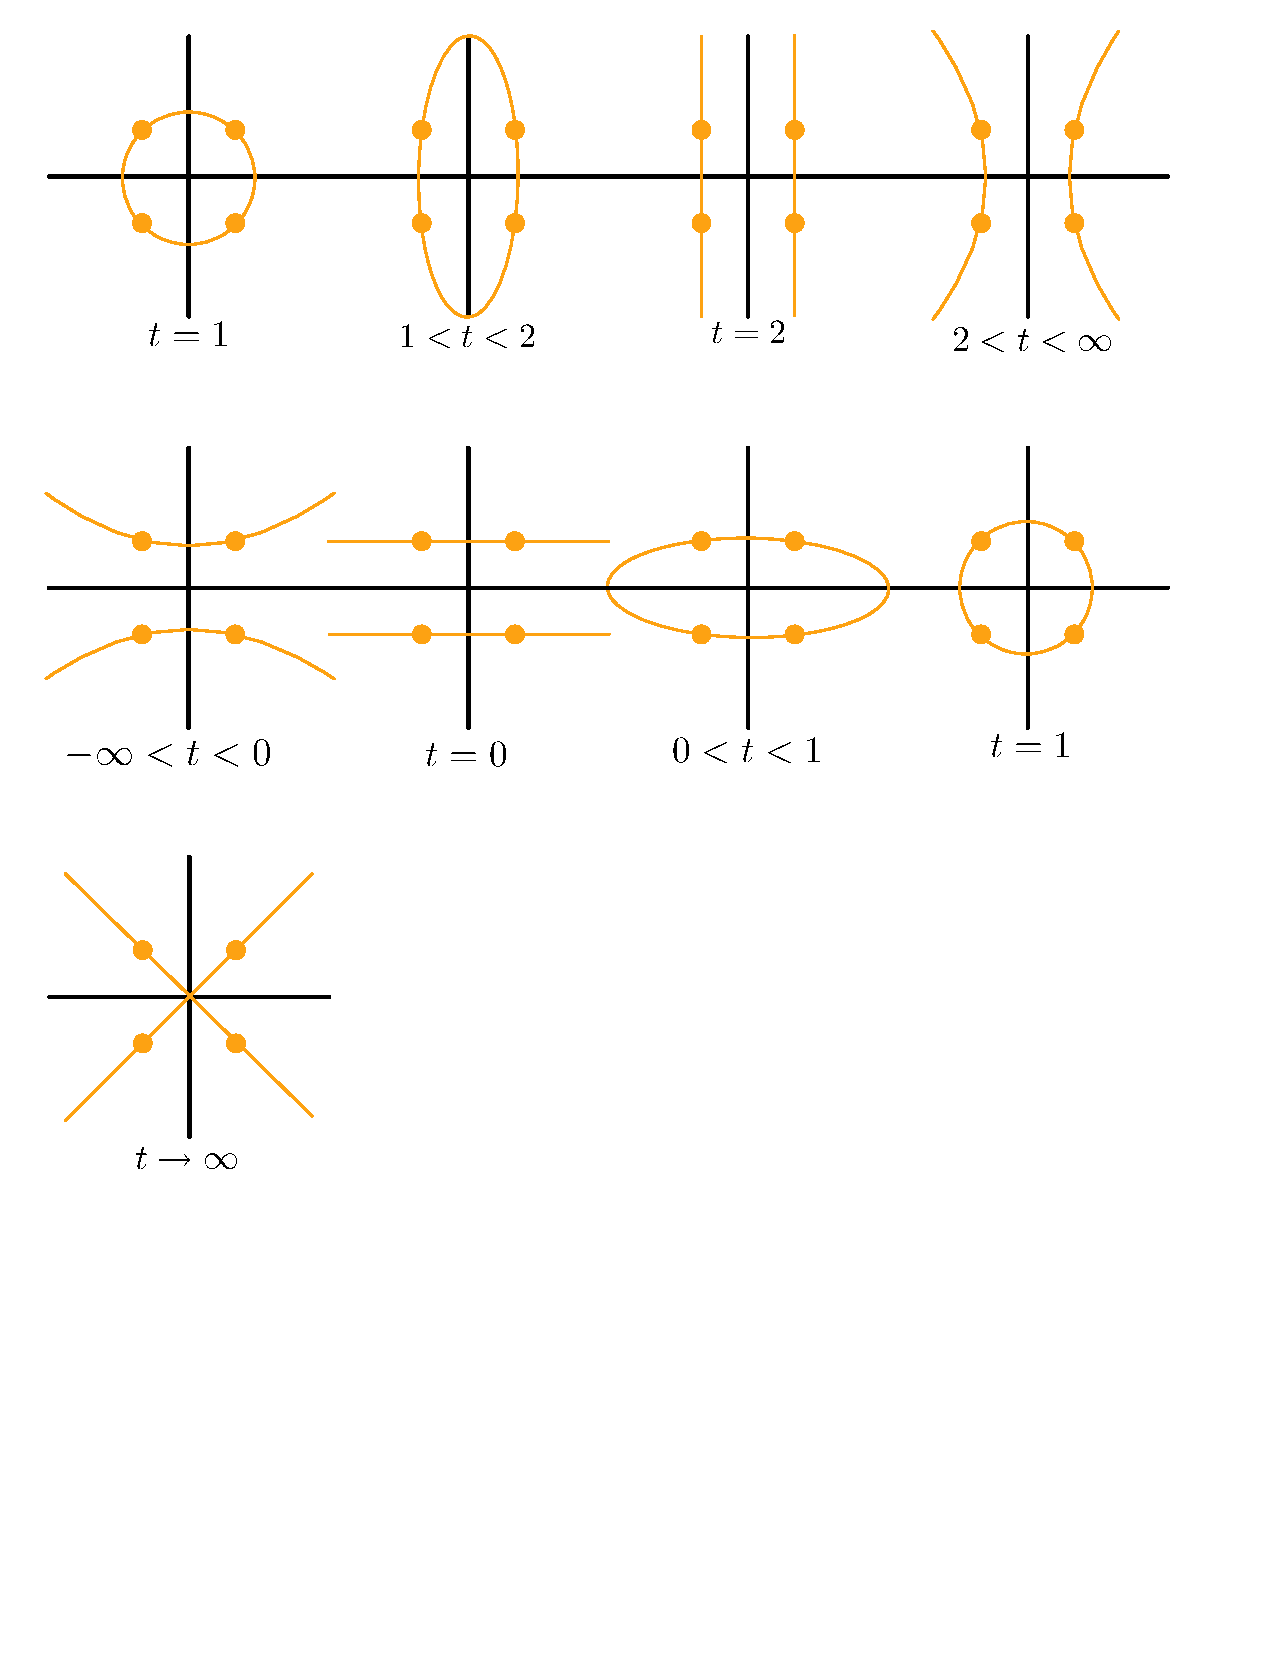
\includegraphics[width=0.3\textwidth, trim= 0.8cm 22.9cm 16cm 0.6cm,clip]{figs/fig1Intro.pdf}
        \label{fig1Intro}
        \caption{One of the quadratic curves passing through our points: $x^2+y^2=2$.}
    \end{figure}\newpage
    Ideally we would like to stretch and shrink the circle in order to make it an ellipse. We know ellipses have equations of the form 
    $$\left(\frac xa\right)^2+\left(\frac yb\right)^2=1,$$ 
    but in order to use our circle equation we will instead add coefficients to the equation in the following fashion
    $$Ax^2+By^2=2.$$
    These coefficients are determined by the points on the curve, we may derive the relation by plugging in the coordinates of a point into the equation:
    $$A(1)^2+B(1)^2=2\To B=2-A\To tx^2+(2-t)y^2=2$$
    where we take $t=A$ to get the last equation.
    The following curves are the ones we obtain given different values of $t$:
    \vspace{-0.5em}
    \begin{itemize}
        \begin{multicols}{2}
            \itemsep=-0.4em
        \item $(t=1)$: A circle.
        \item $(1<t<2)$: An ellipse.
        \item $(t=2)$: The pair of lines $x^2=1$.
        \item $(t>2)$: A hyperbola.
        \end{multicols}
    \end{itemize}
    However we are left with one curve which passes through the points in question. To find it we will assume $t$ is non-zero. From our parametric equation we obtain 
    $$tx^2+(2-t)y^2=2\To x^2+o(t)+y^2=\frac{2}{t}\xrightarrow[t\to\infty]{}x^2=y^2$$
    which is the pair of lines $y=\pm x$. Observe that this behavior is independent of the sign of the infinity we are going to. 
    \begin{figure}[h!]
        \centering
        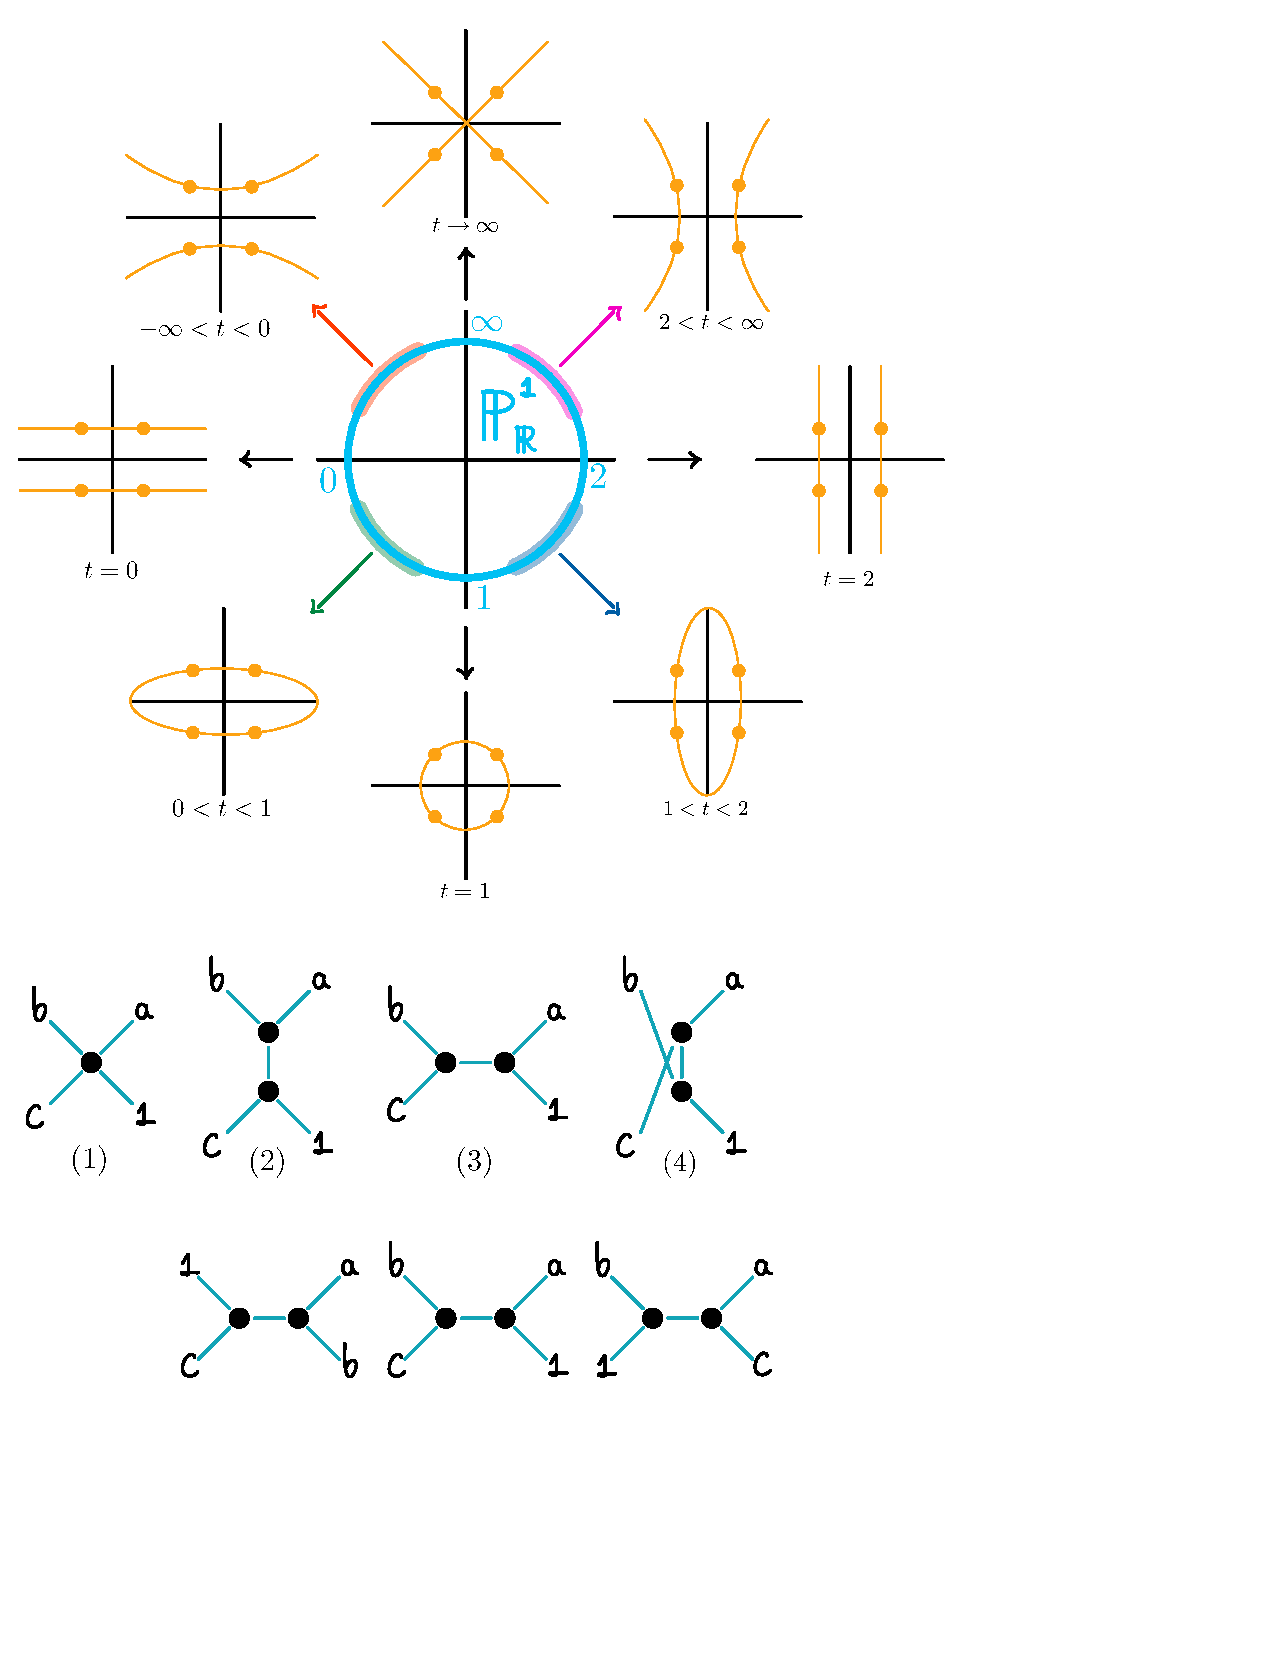
\includegraphics[width=0.8\textwidth, trim= 0.25cm 13.1cm 5.25cm 0.5cm,clip]{figs/fig2Intro.pdf}
        \label{fig2intro}
        \caption{The projective line seen as the moduli space $\ov M_{0,4}$.}
    \end{figure}
    As such, these are all the conics passing through this four points. We omit the complex case in this example but this can be done in full generality.
\end{Ex}
   
    \iffalse
    In essence what we have seen is that all the quadratic curves passing through our set of points can be parametrized by $\bR\cup\set{\infty}$. Formally:
    \begin{Prop}\label{prop:cM04barIsomP1}
    The moduli space $\ov{\cM}_{0,4}$ can be identified with $\bP^1_\bR$.
    \end{Prop}
    Intuitively the moduli space is a set of parameters. When the points vary \emph{continuously}, the objects they parametrize deform \emph{continuously} as well. What we have done here is not a proof of the previous proposition but it may serve as evidence that it is true.\par 
    To study this space and other spaces which may arise in this fashion, we may ask a question like \emph{how many such curves can we find?} In order to do this, we will address this problem by connecting it with graphs. 
    \fi
    \newpage
This example suggests a strategy for solving the original problem for any choice of four points.

\begin{Ex}
    Given four distinct points $A$, $B$, $C$, and $D$ in general position, we look for all the possible conics passing through them.\par
    Define $F$ to be the reducible conic formed by the union of the lines through $A$ and $B$, and $C$ and $D$. Similarly, let $G$ be the conic formed by the lines through $A$ and $C$, and $B$ and $D$. Then the family of conics
    $$\la F+\mu G=0,\quad [\la,\mu]\in\bP^1$$
    describes all conics passing through the four given points.
\end{Ex}



In other words, the space of conics passing through four points in general position is naturally parametrized by $\mathbb{P}^1$. This is an example of a moduli space: a geometric space whose points parametrize certain types of objects. 

\section{A different viewpoint on the same problem}

Kapranov \cite{KapranovPaper} studied spaces which parametrized curves of certain degree passing through a number of points. The problem of classifying conics with marked points is one of such cases, and this transforms into the problem of classifying four-pointed copies of $\bP^1$. There is an equivalence between pointed curves and marked Riemann surfaces. Following this, we will emphasize the viewpoint of marked Riemann surfaces, as it better aligns with the study I have realized. 

\begin{Prop}%%%ADD FIG HERE
    Any smooth conic in the projective plane is isomorphic to the projective line.
\end{Prop}

For our four pointed conic, we get an isomorphic $(\bP^1,p_1,\dots,p_4)$. 

\begin{figure}[h!]
        \centering
        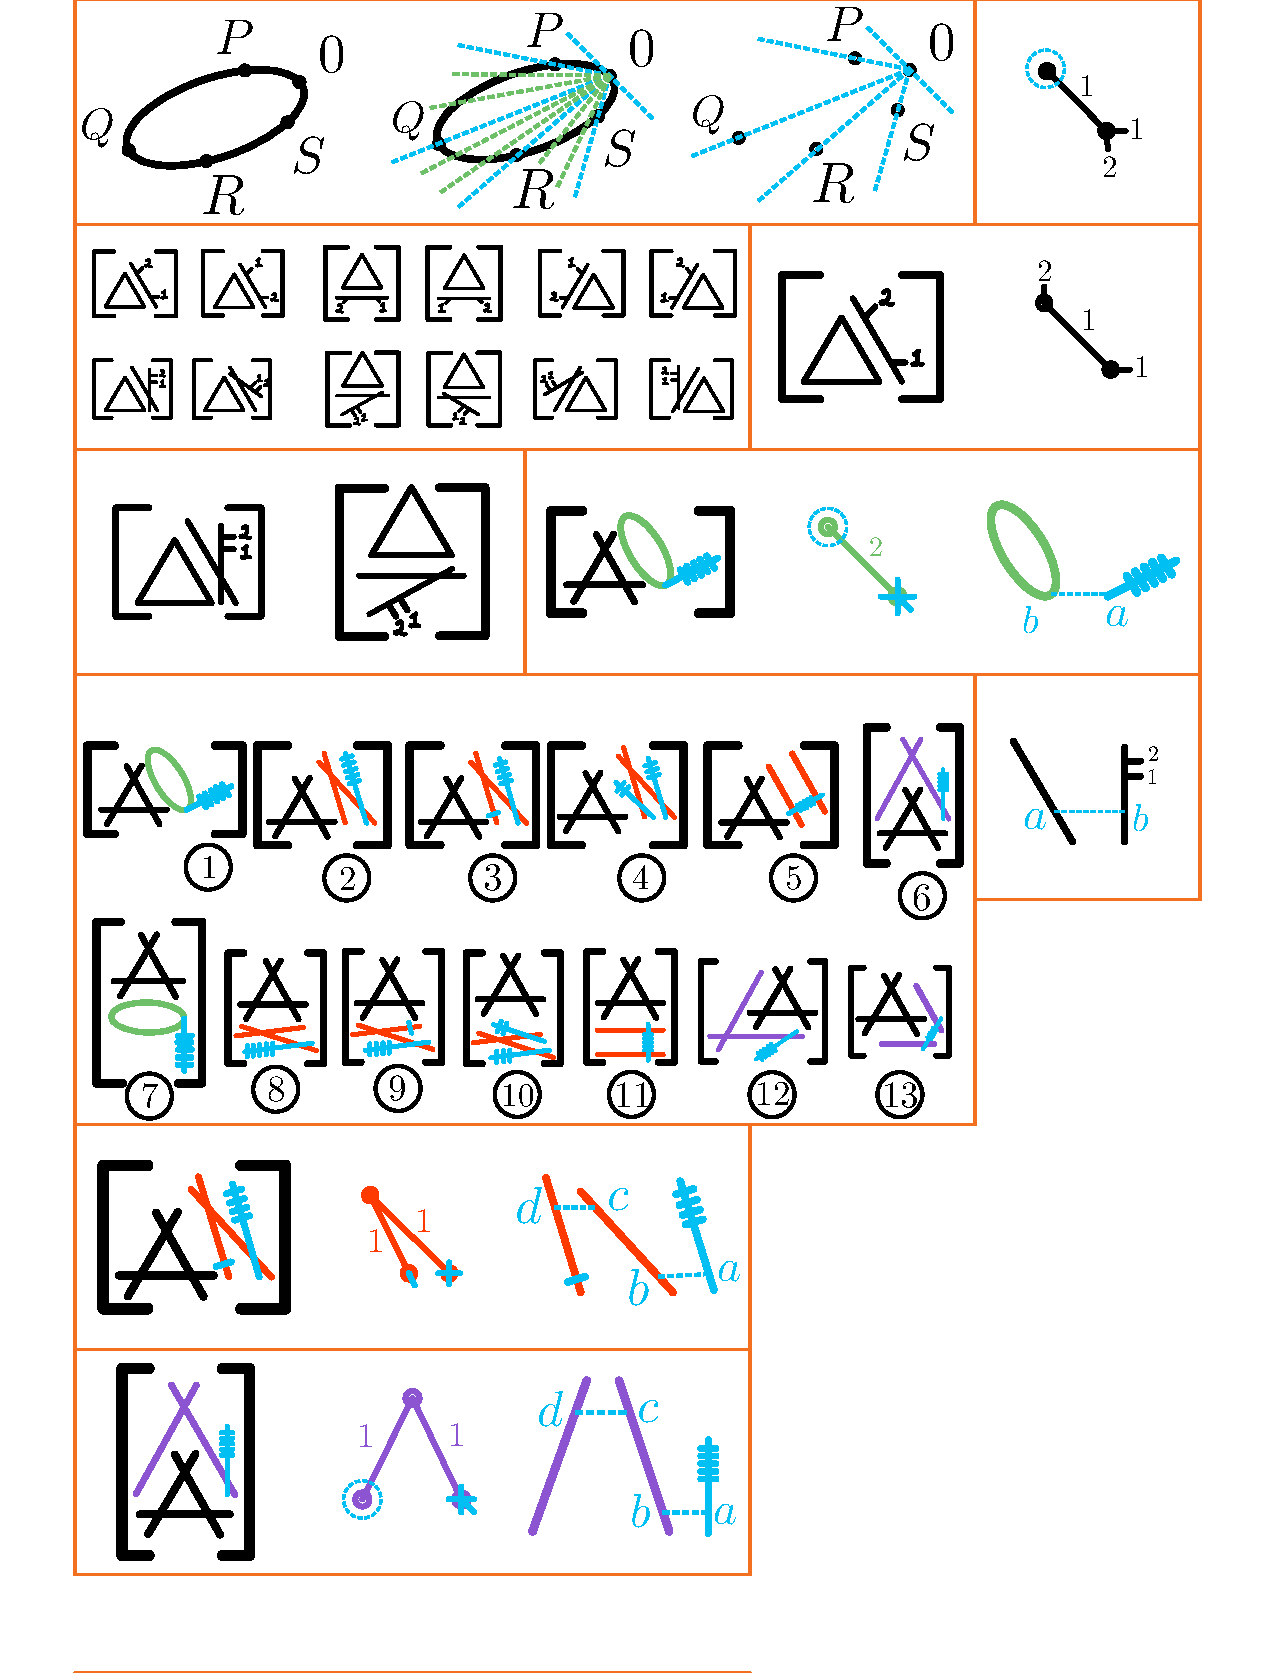
\includegraphics[width=0.9\textwidth, trim= 1.32cm 24.6cm 5.2cm 0.1cm,clip]{../figs/FigsDNnotability3.pdf}
        \caption{Projection from $0$ turns conic into $\bP^1$}
        \label{fig:smooth-conic-into-P1}
    \end{figure}
\begin{ptcb}

    The idea of the proof consists in taking a point in the conic from which we project lines and then create a bijection between this lines and $\bP^1$.\par
    As the conic is smooth, such lines will only have one other point of intersection with the curve meaning that we can find a bijection between points in the conic and points in the projective line.
\end{ptcb}

\begin{Rmk}
Observe that for any given four points, we will recover $\bP^1$ along different tuples of points. When we start varying the points through which the conics pass, we will obtain a different tuple. Our question is then, how do we classify this projective lines along with their points?
\end{Rmk}

\begin{Th}
    The automorphism group of $\bP^1$ is the group of Möbius transformations, $\PGL_2$. Given any two ordered triple of points 
    $$p_1,p_2,p_3\word{and}q_1,q_2,q_3$$
of the projective line, there exists a unique automorphism $T$
 of the projective line such that $T(p_i)=q_i$.
\end{Th}

We will assume the first part of this result and quickly we mention the proof for the second part.

\begin{ptcbp}
Any such automorphism is of the form 
$$z\mapsto \frac{az+b}{cz+d}$$
so let us build a map which takes $p_1,p_2,p_3$ to $0,1,\infty$ (in affine coordinates). Such a map is 
$$z\mapsto\frac{z-p_1}{z-p_3}\left(\frac{p_2-p_3}{p_2-p_1}\right).$$
    This maps $p_1,p_2,p_3$ to $0,1,\infty$ respectively. Call this map $T_p$ and then create a similar $T_q$, the desired function $T$ is $T_q^{-1}T_p$.
\end{ptcbp}

\begin{Def}
    Call the image of the fourth point $p_4$ under the aforementioned map $T_p$, the \term{cross-ratio} of the tuple $(p_1,\dots,p_4)$. 
\end{Def}

For our intents and purposes, the problem changed from
\begin{significant}
    When are two conics passing through 4 points in general position isomorphic?
\end{significant}
to the projective variant 
\begin{significant}
    When are two 4-marked projective lines isomorphic?
\end{significant}
And with the previous result we can give the answer. 

\begin{Th}
    The isomorphism class of $(\bP^1,0,1,\infty,t)$ is determined by the value $t\in\bP^1\less\set{0,1,\infty}$. 
\end{Th}

 Each smooth conic then corresponds to a $(\bP^1, 0, 1, \infty, t)$ where $t$ varies in $\bP^1 \less \set{0,1,\infty}$. Intuitively for now we will call it the moduli space of $4$-pointed $\bP^1$'s, $M_{0,4}$.\par

 But observe we are missing two things, only one of which we have talked about before. The new missing aspect is the lack of compactness of this space. $\bP^1$ as a whole is compact, but removing three points also removes that property.\par
 The other missing objects are the \emph{singular} conics. Asking where they went is like asking ``what if we let $t$ go to any of the three special points?'' We will defer the interested reader to Kock and Vainsencher's \emph{Green Book} \cite{GreenBookKockVainsencher} to fill out the details of the universal family business. In our treatment it suffices to know that whenever two points collide, we will blowup $\bP^1$ at that point adding an exceptional divisor isomorphic to $\bP^1$ and then adding the two marked points there.\par
 This treatment guarantees that $\ov M_{0,4}$ is now compact and so we have a nicer moduli space. Let us now delve deeper into this notion and throughly explain how we added the singular conics.

%%%%Aquí iba el family business

\section{Moduli of curves}

As a quick refresher, let us clarify the objects which are parametrized by the moduli spaces of our interest. 

\begin{Def}
    A \term{Riemann surface} is a complex analytic manifold of dimension $1$. 
\end{Def}

For every point in the surface, there's a neighborhood which is isomorphic to $\bC$ and transition functions are linear isomorphisms of $\bC$. We will interchangeably say Riemann surface or \emph{smooth compact complex curve}.
    
\begin{Ex}
        The following classes define Riemann surfaces.
        \begin{enumerate}
        \item $\bC$ itself is a Riemann surface with one chart.
        \item Any open set of $\bC$ is a Riemann surface.
        \item A holomorphic function $f\: U\subseteq\bC\to\bC$ defines a Riemann surface by considering $\Ga_f\subseteq\bC^2$. There's only one chart determined by the projection and the inclusion $i_{\Ga_f}$ is its inverse.
        \item Take another holomorphic function $f$, then $\set{f(x,y)=0}$ is a Riemann surface such that 
        $$\text{Sing}(f)=\set{\del_xf=\del_yf=f=0}=\emptyset.$$
        This means that at every point the gradient identifies a normal direction to the level set $f=0$. In particular, there's a well defined tangent line. The inverse function theorem guarantees that this is a complex manifold. 
        \item The first compact example is $\bP^1$.
        \end{enumerate}
\end{Ex} 

\begin{Def}
    The \term{moduli space} $M_{g,n}$ is the set of isomorphism classes of genus $g$, $n$-pointed Riemann surfaces.
\end{Def}

Recalling our motivating example, we called the space which classified the conics $M_{0,4}$. According to this definition, we are classifying $4$-pointed genus 0 Riemann surfaces. It is indeed the case that $\bP^1$ is the unique up-to-isomorphism Riemann surface of genus 0. Let us explore what happens in further genus higher up.

\begin{Ex}
    The space $M_{1,1}$ parametrizes $1$-pointed genus $1$ Riemann surfaces, or 1-marked \emph{elliptic curves}.\par
    Any such curve is isomorphic to 
    $$\quot{\bC}{L},\quad L=\bZ u+\bZ v,\word{where}u,v\in\bZ,$$
    and the image of the origin under the quotient map is the natural choice for the marked point. We have that two lattices $L_1,L_2$ determine the same elliptic curve whenever 
    $$\exists \al\in\bC^\x(L_2=\al L_1).$$
    So that 
    $$M_{1,1}=\quot{\set{\text{lattices}}}{\bC^\x}$$
    but we can be more precise!\par
    Explicitly, a lattice $L=\gen_\bZ(u,v)$ can be rescaled to
    $$\tilde{L}=\frac{1}{u}L=\gen_\bZ(1,\tau).$$
    This quantity $\tau$ always lies in the upper half plane when 
    $$\arg(v)>\arg(u)\bmod[-\pi,\pi]$$
    which means that $\tau\in\bH$ parametrizes $\bonj{\quot{\bC}{L}}$. 
    Let us apply two $\rSL_2(\bZ)=\gen(S,T)$ actions on $\tau$ which will leave the quotient unchanged:
    $$
    \left\lbrace
    \begin{aligned}
        &T\:\tau\mapsto\tau+1=\twobytwo{1}{1}{0}{1}\circ\tau=\frac{\tau+1}{0+1},\\
        &S\:\tau\mapsto-\frac1\tau=\twobytwo{0}{-1}{1}{0}\circ\tau=\frac{0-1}{\tau+0}.
    \end{aligned}
    \right.
    $$
    Then observe that the lattices
    $$\gen_\bZ(1,T\.\tau)\word{and}\gen_\bZ(1,S\.\tau)$$
    give us the same quotient. From this we can be more specific and say
    $$M_{1,1}=\quot{\bH}{\rSL_2(\bZ)}.$$
\end{Ex}

Once again, we arrive at the same issue that this space is not compact. Last time we found a way to compactify the space by adding some \emph{evidently} missing points. But it is unclear here how to deal with this conundrum. We address the problem by introducing the notion of stability.

\subsection{Stable curves}

\begin{Def}[\cite{ZvonkineIntro}, pg. 16]
    A genus $g$, $n$-pointed \term{stable curve} $(C,p_1,\dots,p_n)$ is a compact complex algebraic curve satisfying:
    \begin{enumerate}
        \item The only singularities of $C$ are simple nodes.
        \item Marked points and nodes are all distinct. Marked points and nodes do not coincide.
        \item\label{fin-number-auts} $(C,p_1,\dots,p_n)$ has a finite number of automorphisms.
    \end{enumerate}
    Throughout, we assume that stable curves are connected. The \emph{genus} of $C$ is the arithmetic genus, or equivalently, the genus of the curve obtained when \emph{smoothing the nodes}.
\end{Def}

\begin{Rmk}
Observe that the definition calls the object an \emph{algebraic curve} and not a manifold. It's almost a manifold, but it's not because it can lack smoothness.
\end{Rmk}

From here on, we can talk about $\ov{M}_{g,n}$, the moduli space of stable, genus $g$, n-pointed curves. The technicalities of whether this space is actually an orbifold or a stack will not concern us in this work. 

\begin{Prop}\label{prop-dim-Mgn}
    The dimension of $\ov{M}_{g,n}$ is $3g-3+n$.
\end{Prop}

Originally, Riemann showed that the dimension of the space without marks is $3g-3$. The proof goes along the lines of finding the dimensions of a Picard group, a Hurwitz space and a particular Grassmannian. The moduli space can be located in a diagram involving all of these spaces and thus its dimension can be found. There's modern approaches to this count but this is the core of Riemann's original idea. Adding marks just adds a degree of freedom per mark so that we get the extra $+n$ in dimensions.\par
Let us condense the criterion of finite number of automorphisms into a single, easy-to-spell-out idea which will be of use.

\begin{Th}[\cite{ZvonkineIntro}, pg. 17]\label{th-stability-condition-22gn}
A stable curve admits a finite number of automorphisms (as in condition \ref{fin-number-auts}) if and only if every connected component $C_i$ of its normalization with genus $g_i$ and $n_i$ \emph{special} points satisfies 
$$2-2g_i-n_i<0.$$
\end{Th}

\begin{Rmk} %%%Add figure of normalization
    %https://en.wikipedia.org/wiki/Zariski%27s_main_theorem
    %https://mathoverflow.net/questions/109395/is-there-a-geometric-intuition-underlying-the-notion-of-normal-varieties
    %https://en.wikipedia.org/wiki/Normal_scheme
\begin{figure}[h!]
        \centering
        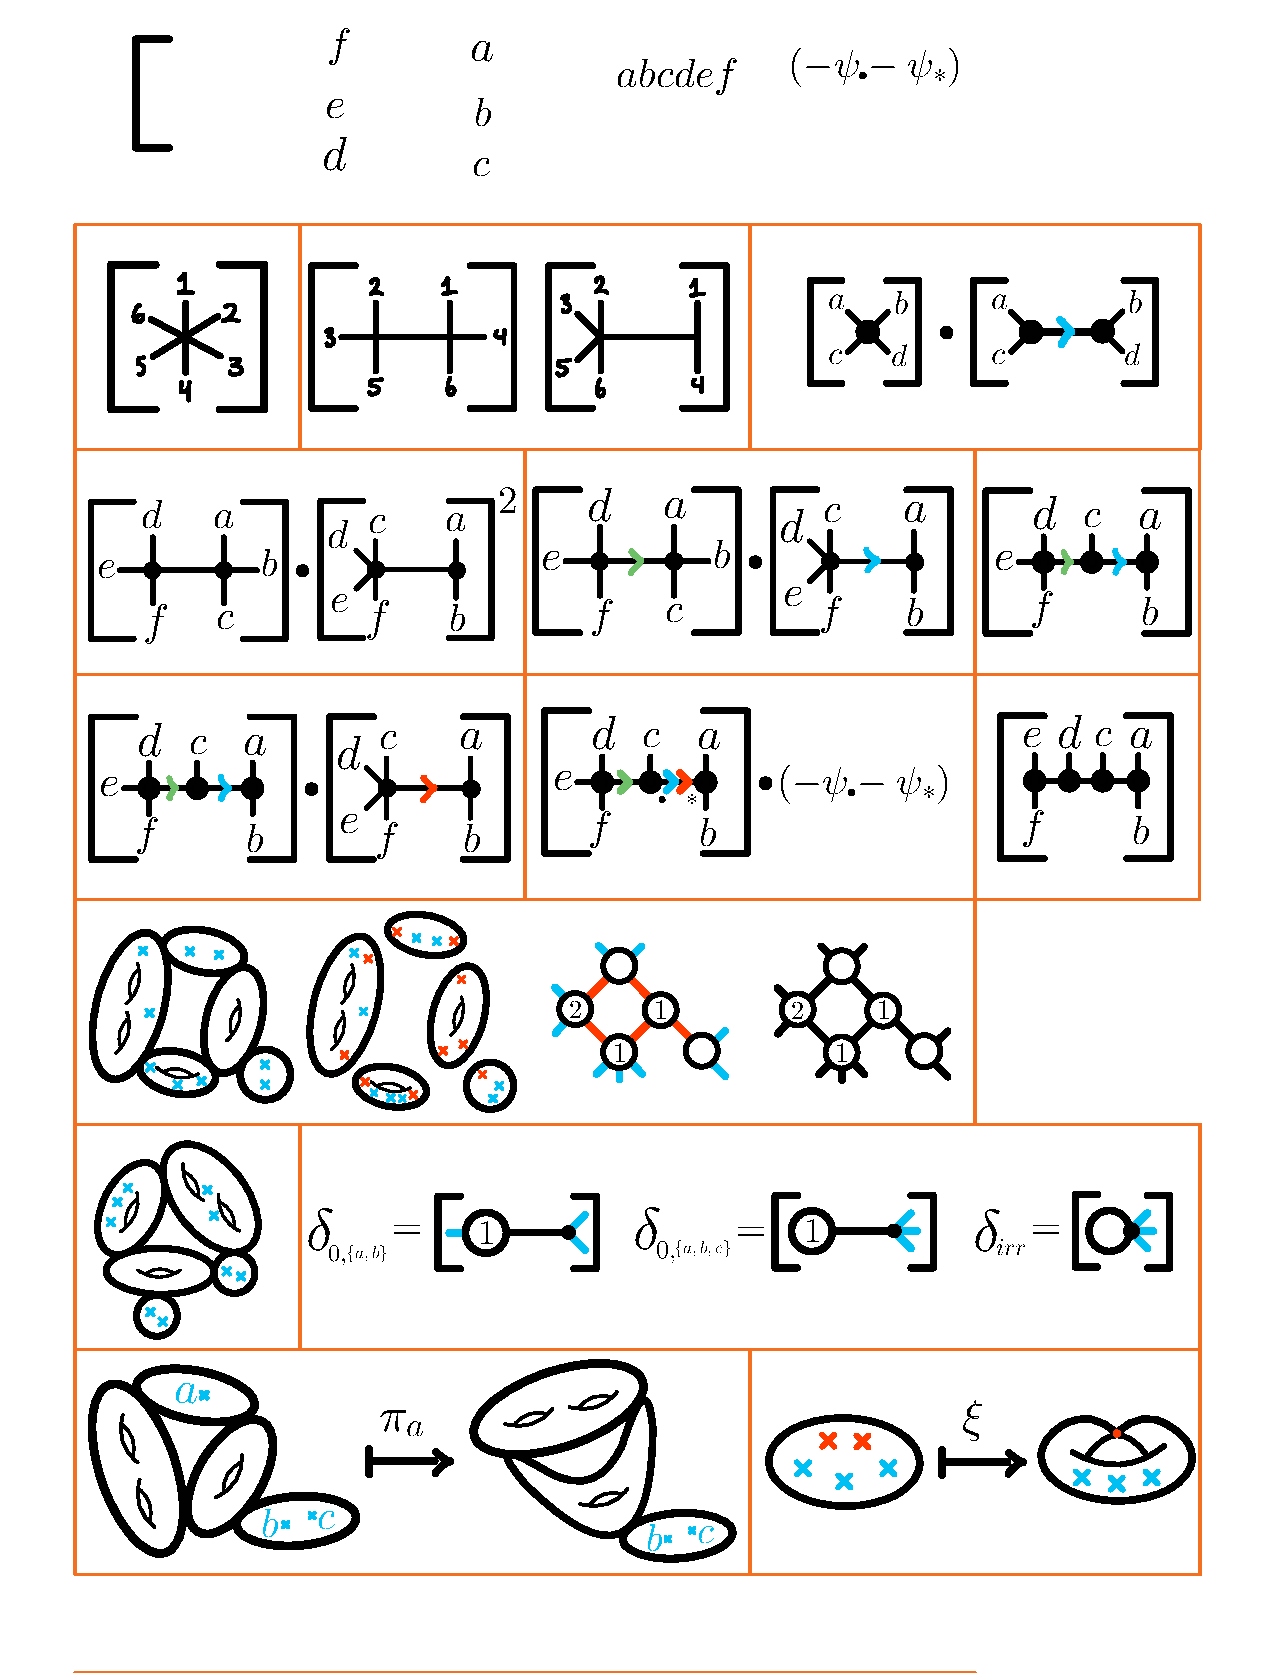
\includegraphics[width=0.6\textwidth, trim= 1.32cm 9.5cm 12.7cm 15.4cm,clip]{../figs/FigsDNnotability1.pdf}
        \caption{Nodal curve and its normalization}
        \label{fig:normalization-example}
    \end{figure}
Normalization can be intuitively understood as the process of ``ungluing'' a variety at its singularities.\par
Formally, the normalization of a variety $X$ is a non-singular (possibly disconnected) variety $\widetilde X$ equipped with a finite birational morphism 
$$\nu:\widetilde X\to X.$$
This map is an isomorphism over the smooth locus of $X$ but may identify several points in $\widetilde X$ over a singular point of $X$. Thus, we may think of $\widetilde X$ as a version of $X$ in which the undue gluings of subvarieties. In the case of curves, normalization replaces each node with two distinct smooth points, resulting in a smooth curve (or collection of curves) marked by the preimages of the nodes. 
\end{Rmk}

\begin{ptcb}
    We will discuss that whenever the inequality holds, we have the components of the curve have finitely many automorphisms.\par
    Starting by considering the $g=0$ case, we may see that whenever $n\geq 3$ we have $\bP^1$'s with at least 3 marks. Thus there's no automorphisms besides the identity as any such map should fix three points.\par
    For the case of $g=1$, the inequality holds when $n$ is at least 1 as well. In this case, the only automorphism corresponds to the elliptic involution.\par
    And for $g>2$, we only need consider the hyperelliptic involution.
    %look at \href{https://math.stackexchange.com/questions/1680144/automorphism-group-of-genus-2-curve}{mse/1680144}
    %\red{Consider hyperelliptic involution}.
    These three conditions are summarized in the inequality $2-2g_i-n_i<0$.
\end{ptcb}
\begin{Ex}
    Observe that following our motivational example, we get to the three stable curves in $\ov M_{0,4}$. Each one of these is a nodal curve where the marks and the node differ. And applying the theorem, we see that each component of the normalization satisfies
    $$2-0-3=-1<0$$
    so that we do have the stability condition. 
\end{Ex}

\begin{Ex}\label{ex-Mg1n1-compactification}
    For the case of $M_{1,1}$, we compactify by adding a point representing singular stable curve. This is a one-point $\bP^1$ where we attach two points together. The resulting curve has arithmetic genus one. It can be also imagined as ``pinching a loop around the torus which doesn't go around the hole''. This is once again a stable curve as we have the stability condition:
    $$2-2(1)-1=-1<0.$$
\end{Ex}

Once equipped with the idea of stability we can now calmly talk about $\ov M_{g,n}$ as the set of isomorphism classes of \emph{stable curves}. This space can be treated as an orbifold (as in Zvonkine's article \cite{ZvonkineIntro}), as a Deligne-Mumford stack, but we will not deal with such intricacies here. Instead, we will now delve into the cohomology of this space and talk about the combinatorial tools that will help us further along the road.

\section{Cohomological classes of the moduli space}

\subsection{The Chow ring}
%Thanks to Richard E. Borcherds here
Intuitively, for a non-singular variety $V$, we define the \emph{Chow ring} $A^\ast(V)$, whose elements \emph{correspond} to subvarieties of $V$, and the product reflects the intersection of these subvarieties. The ring is graded by codimension:
$$A^\ast(V) = \bigoplus_i A^i(V)$$
where $A^i(V)$ consists of classes of subvarieties with codimension $i$. Ideally, the intersection of a codimension $m$ subvariety $X$ and a codimension $n$ subvariety $Y$ would yield a subvariety of codimension $m+n$.\par
However, this does not always hold. Imagine a hyperplane $H$ intersected with itself. So there's a complication in defining this product.

\begin{Def}
    The $i$-th \term{Chow group} $A^i(V)$ of a non-singular variety $V$ consists of equivalence classes of codimension $i$ cycles, where two cycles are equivalent if their difference is a principal divisor, i.e., the zero set of a rational function.
\end{Def}

The \term{Chow ring} is the direct sum over all Chow groups:
$$A^\ast(V) = \bigoplus_i A^i(V)$$
The intersection product on the Chow ring is well-defined:
$$[X] \cap [Y] = \sum_{[Z]} i(X, Y; Z) [Z]$$
where $[X]$, $[Y]$, $[Z]$ denote rational equivalence classes of cycles, and $i(X, Y; Z)$ is an \emph{intersection number}, representing the multiplicity of the intersection at $Z$.

\begin{Rmk}
In the cases when we do have a transversal intersection between $X$ and $Y$, it holds that 

$$
\left\lbrace
\begin{aligned}
&[X]\cap[Y]=[X\cap Y],\\
&\codim(X\cap Y)=\codim(X)+\codim(Y).
\end{aligned}
\right.
$$

\end{Rmk}

\begin{Rmk}
    The Chow ring is related to the cohomology ring via a homeomorphism 
    $$A^i(V)\to H_{2n-2i}(V)\to H^{2i}(V)$$
    where the first map is is the cycle map, and then we apply Poincaré duality. Further exploration of the question as to where the Chow group lies inside the cohomology leads to the Hodge conjecture.
\end{Rmk}

Given the previous, we will indistinguishably call subvarieties \emph{cohomology classes of their respective codimension}. Only the basic idea of what the Chow ring as a set of isomorphism classes of subvarieties is and the idea that intersection of subvarieties corresponds to the product inside the Chow ring is essential.

\subsection{Chern classes}

Similar to the basics of the Chow ring, we will be reviewing the following properties about Chern classes. These are a particular case of characteristic classes which are elements of the cohomology of the base of a vector bundle $E\xrightarrow[]{\pi}B$. The precise definition of what a Chern class is is not necessary. 

\begin{Th}[Chern classes cheat sheet]\label{th-chern-class-cheat-sheet}
    Suppose $E\xrightarrow{\pi}B$ is a rank $r$ vector bundle. We have the following:
\begin{itemize}
    \item $c_i(E)\neq 0$ whenever $0\leq i\leq r$.
    \item $c_i(E)$ has degree $i$ in the Chow ring. This means $c_i(E)\in A^i(B)$.
    \item $c_0(E)=1$ is the fundamental class. It's usually the case that we rescale in order for this to be exactly $1$.
    \item If we define 
    $$c_{\text{tot}}=c_0+c_1+\dots+c_r$$
    and we have a short exact sequence of vector bundles 
    $$0\to F\to E\to Q\to 0,$$
    then $c_{\text{tot}}(E)=c_{\text{tot}}(F)\.c_{\text{tot}}(Q)$. In particular we have 
    $$c_1(E)=c_1(F)+c_1(Q).$$
    \item If $E$ is a line bundle $L$, i.e. rank 1, then 
    $$c_1(L)=[\div(s)],$$
    this is the class of the divisor of a meromorphic section.
    \item In general, \term{Euler class} is
    $$e(E)\defeq c_r(E)=[Z(s)]-[P(s)].$$%=\bonj{\div(s)},$$
    Here $s$ is a section which in local coordinates may be expressed as 
    $$s=(s_1,...,s_r)$$
    and so $Z$ represents the class of zeroes, while $P$ is the class of poles of the section.
    \item Chern classes commute with pullbacks.
\end{itemize}

Further details and extended properties of Chern classes can be found in the following two references: \href{https://math.stackexchange.com/questions/989147/}{this post in math.stackexchange}\footnote{\href{math.stackexchange.com/q/989147/}{\ttt{math.stackexchange.com/q/989147/}}} or \href{https://rigtriv.wordpress.com/2009/11/03/chern-classes-part-1/}{this post by Charles Siegel}\footnote{\href{https://rigtriv.wordpress.com/2009/11/03/chern-classes-part-1/}{\ttt{https://rigtriv.wordpress.com/2009/11/03/chern-classes-part-1/}}}.

\end{Th}
\subsection{Dual graphs}

We will be describing the cohomology classes of $\ov M_{g,n}$ via their combinatorial data. Each curve has a naturally associated dual graph which we will get to following the ideas of Schmitt and van Zelm \cite{SchmittVanZelm}. The idea of stable graph was initially formalized by Graber and Pandhariphande \cite{GraberPandharipande} and then developed further by Yang \cite{YangIntersections}.\par

\begin{Def}
    A \term{simple graph} $G$ is a pair of sets $(V,E)$ such that  
    $$G=(V,E),\quad E\subseteq\binom{V}{2}=\set{X\subseteq V\:\lvert X\rvert=2}.$$
    The set $V$ is called the set of vertices and elements of $E$ are edges.
\end{Def}
This is equivalent to the following:
\begin{itemize}
    \item $E$ is the graph of a symmetric relation in $V$.
    \item  Schmitt and van Zelm take this characterization to be a map 
$$s:E\to\Sym^2 V=\quot{V\ox V}{u\ox v-v\ox u}.$$
\end{itemize} 

More generally we can look for graphs which have multiple edges between vertices and loops around one vertex.

\begin{Def}
A \term{multigraph} is a graph $G$ in which $E$ and its elements can be multisets. This allows for multiple edges and loops respectively.    
\end{Def}

The Schmitt and van Zelm condition allows this automatically.

\begin{Def}
    A vertex/edge-\term{labeling} by integers is a function from $V$ or $E$ to $\bZ_{\geq 0}$ respectively. 
\end{Def}

As our curves will be marked, we would like to denote that in a graph. The way to do this is via a set of \emph{half-edges} or \emph{legs}. 
\begin{Rmk}
    Graphs can be defined by only specifying a set of half-edges and declaring certain properties. While not pursuing that approach, we refer the reader to a discussion on defining graphs in that manner.\footnote{See more in \href{https://math.stackexchange.com/q/2678435}{\ttt{math.stackexchange.com/q/2678435/}}.}. 
\end{Rmk}
Following Schmitt and van Zelm we take the idea of half-edges to define stable graphs.

\begin{Def}
A \term{stable graph} $\Ga$ is a tuple of sets and maps:
$$\Ga=(V,H,L,g,\iota,a,\ze)$$
where $V$ is the set of vertices, $H$ the set of half-edges and $L$ is the set of legs. We have the following conditions:
\begin{enumerate}
    \item The map $g\: V\to\bZ_{\geq 0}$ is a labeling of the vertices to denote their genus.
    \item $\iota\: H\to H$ is a fixed-point free involution, intuitively switching ends of a edge.
    \item The map $a\: H\to V$ assigns half-edges to vertices.
    \item The map $\ze\: L\to V$ assigns the legs to the vertices.
    \item The orbits of $\iota$ form the edges via the induced function by $a$ on $E$.
    \item And each vertex $v$ satisfies the condition
    $$2-2g(v)-\lvert a^{-1}(v)\rvert-\lvert \ze^{-1}(v)\rvert<0.$$
\end{enumerate}    
We may call $n(v)\defeq\lvert a^{-1}(v)\rvert+\lvert \ze^{-1}(v)\rvert$ the valence\footnote{In graph theory this quantity is called the degree of a vertex. However, to avoid ambiguity when discussing morphisms, we refer to it here as the valence.} of the vertex $v$. This is number of half-edges and legs incident in $v$. 
\end{Def}

Observe immediately the similarity between the last condition in the stable graph definition and the stability condition for curves in theorem \ref{th-stability-condition-22gn}. 
If the definition sounds too technical it's because it is! We should carry in our minds that a stable graph is labeled multigraph which satisfies the stability condition. Let's now associate a graph to a curve.

\begin{Def}
    The \term{dual graph} $G$ of the curve $(C,
p_1,\dots,p_n)$ is built from its normalization $N$. 
\begin{itemize}
    \item The vertices of $G$ correspond to each connected component of $N$:
    $$V(G)=\set{X_i\: X_i\word{is a connected component of}N}.$$
    Each vertex has an associated genus $g_v$ equal to the genus of the component $X_i$.
    \item The half-edges correspond to points in each component mapping to the same node in $C$.
    \item $L$ corresponds to the marked points.
    \item The genus function $g$ is the genus of $X_i$.
    \item $\iota$ transposes points mapping to the same node.
    \item $a$ and $\zeta$ identify to-be nodes and marks with component they lie on.
\end{itemize}
\end{Def}

\begin{Ex}\label{ex-random-curve-ovM49}
    Consider the following curve in $\ov M_{4,9}$ along its normalization.
    \begin{figure}[h!]
        \centering
        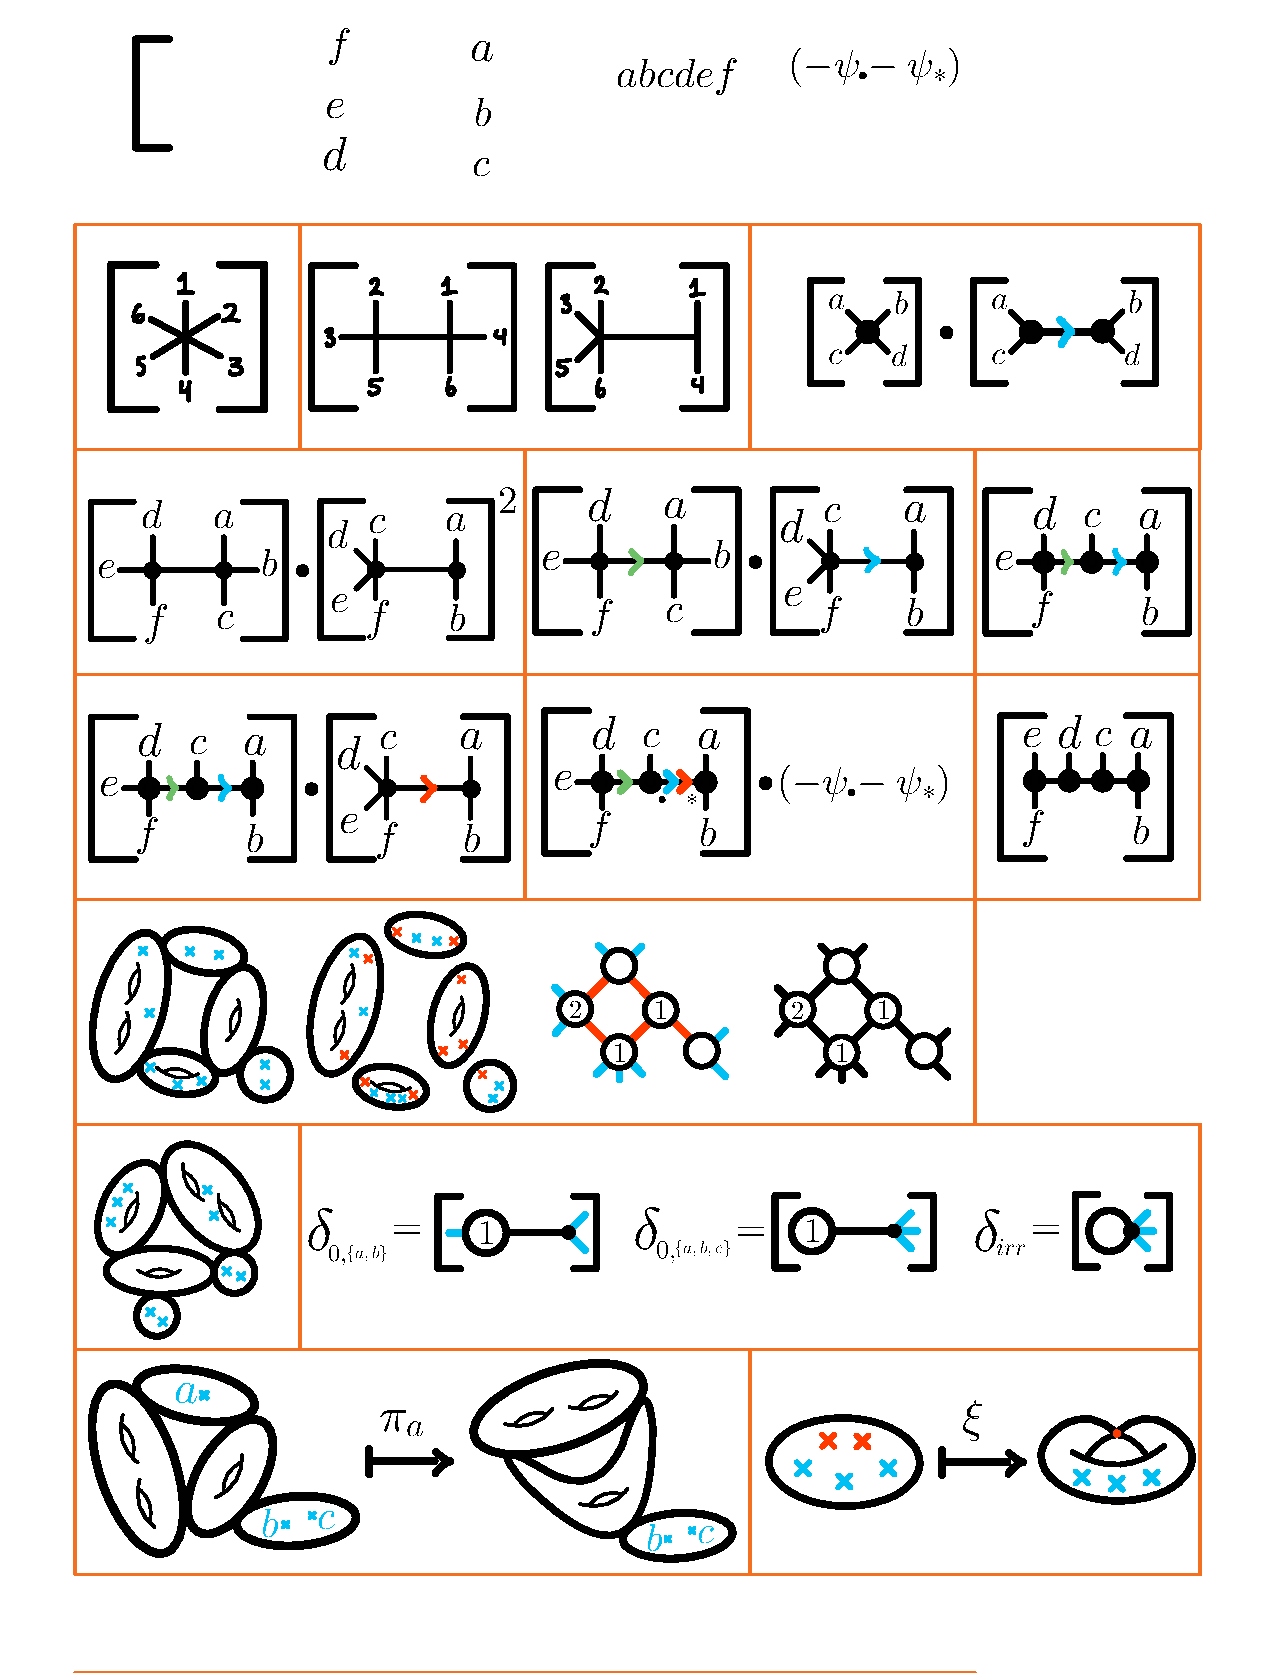
\includegraphics[width=0.6\textwidth, trim= 1.32cm 9.5cm 12.7cm 15.4cm,clip]{../figs/FigsDNnotability1.pdf}
        \caption{Unlabeled nodal curve in $\ov M_{4,9}$}
        \label{fig:unlabled-random-curve-ovM49}
    \end{figure}
    We have omitted the labeling on the markings for now but we have distinguished the special points on each component by coloring nodes red and markings blue. We now build the corresponding dual graph following the aforementioned procedure.
    \begin{figure}[h!]
        \centering
        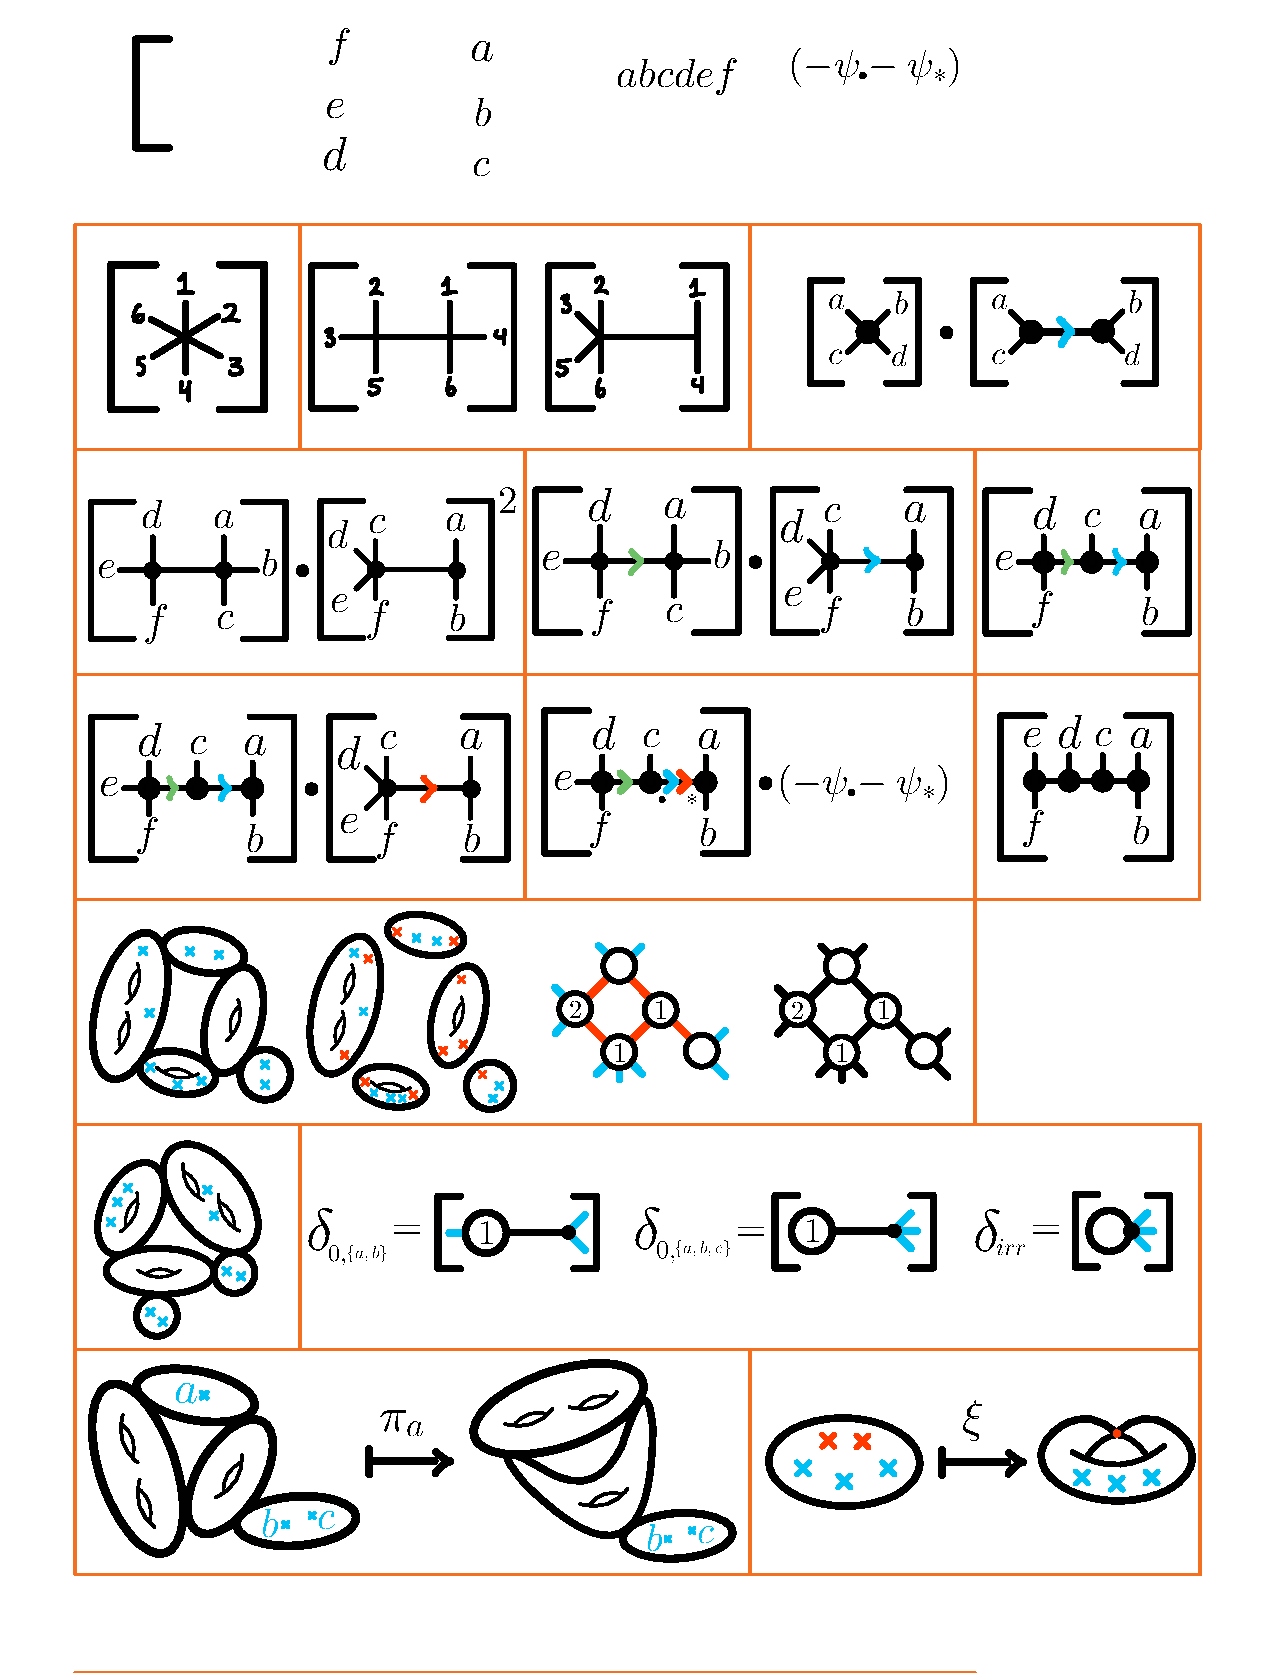
\includegraphics[width=0.6\textwidth, trim= 9.3cm 9.9cm 5.45cm 15.9cm,clip]{../figs/FigsDNnotability1.pdf}
        \caption{Dual graph corresponding to the curve in figure \ref{fig:unlabled-random-curve-ovM49}}
        \label{fig:unlabled-random-curve-ovM49-graphs}
    \end{figure}
    In the first graph we have color-coded the information by coloring the edges red and the half-edges blue. More usually than not, we will draw the graphs as the one on the right possibly including labels for the marks.
\end{Ex}

The following result will come in handy to categorize where in the Chow ring of $\ov M_{g,n}$ does a particular graph live.
\begin{Th}
    The codimension of a marked curve $C$ is the number of nodes it has. This is the number of edges that its dual graph has.
\end{Th}

After pondering this result and looking at the previous example we may think of the question about what happens when two curves have the same dual graph. For that, we consolidate in the following definition.

\begin{Def}
    A \term{stratum} in $\ov{M}_{g,n}$ is the closure of the set of all curves with the same topological type. Strata are classified by dual graphs. 
\end{Def}

These strata are what we will use to organize data inside the Chow ring. For a curve $C$, we will talk about the class $[C]\in A^\ast(\ov M_{g,n})$ as the cohomology element representing it. 

\begin{Ex}
    So taking into account the previous curve from example \ref{ex-random-curve-ovM49}, consider also the next curve. 
    \begin{figure}[h!]
        \centering
        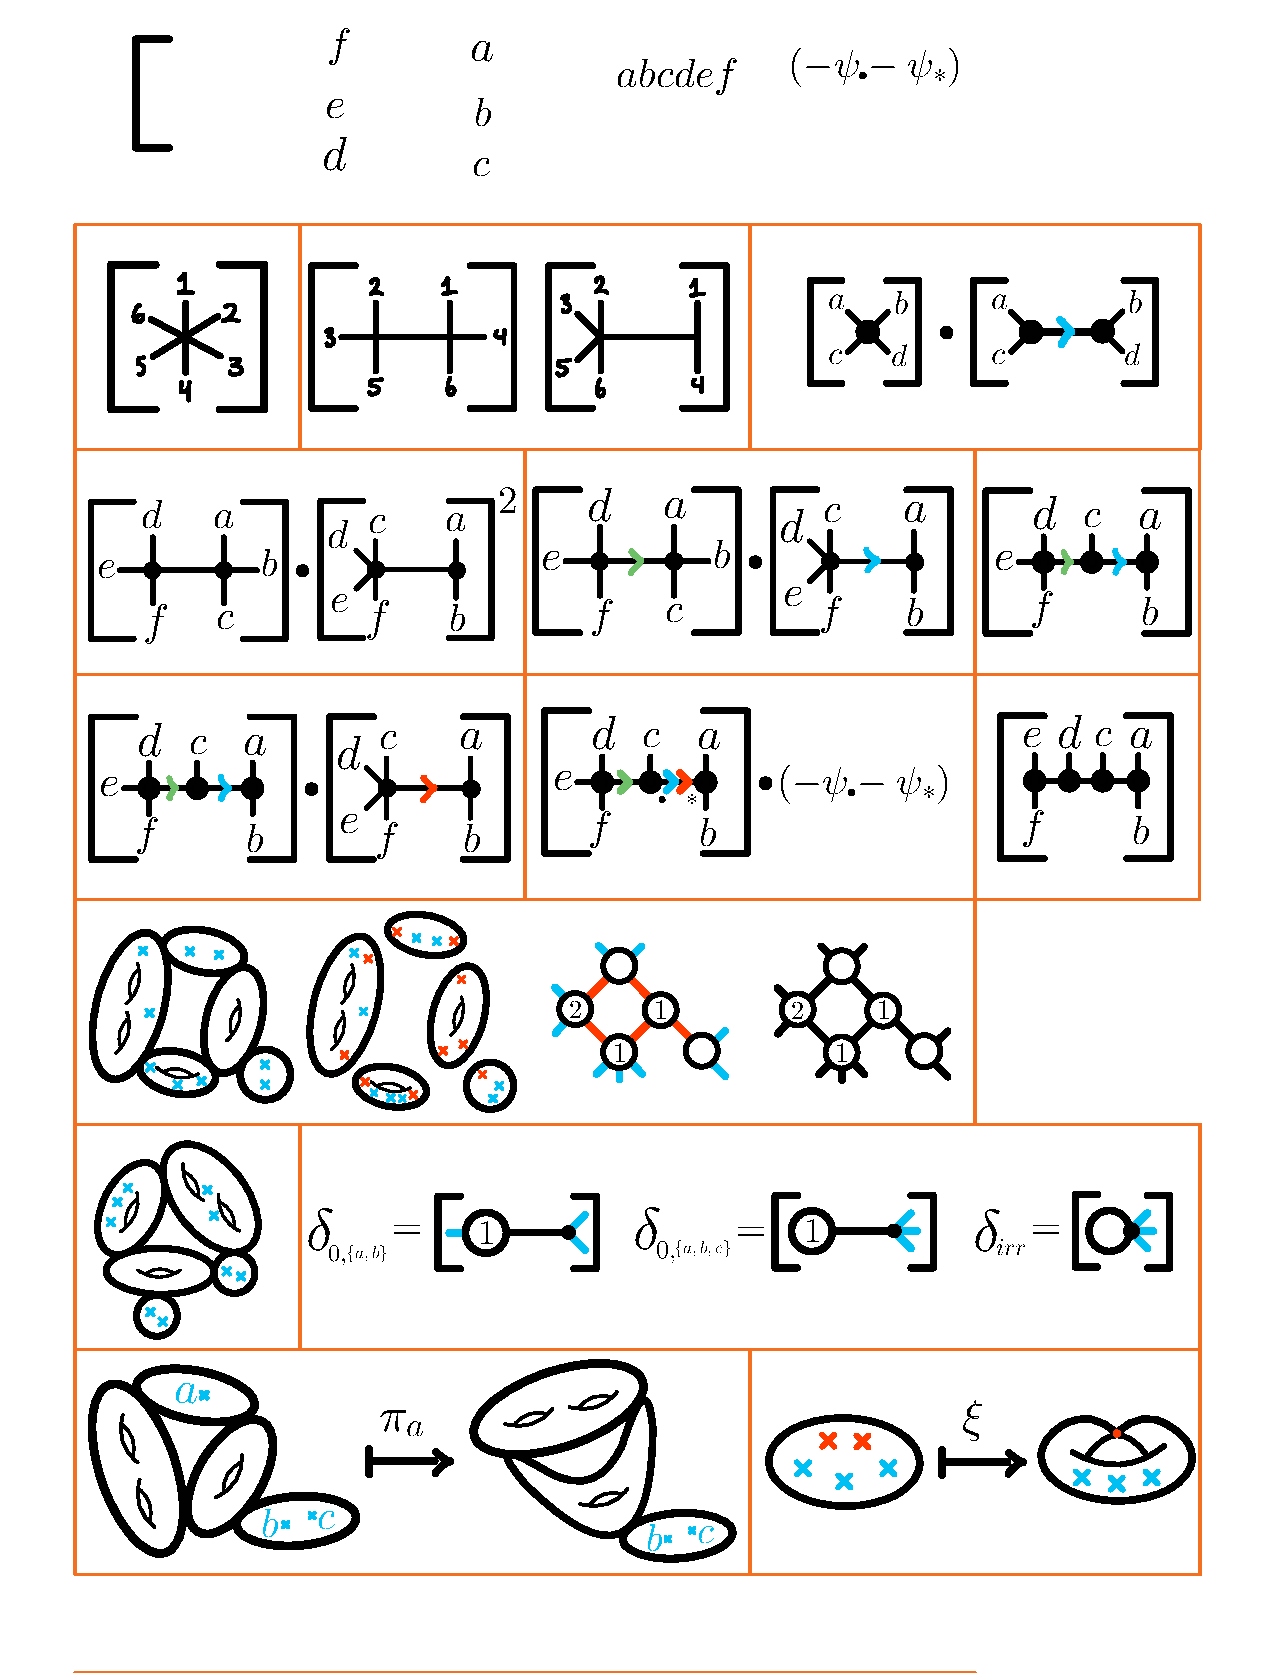
\includegraphics[width=0.3\textwidth, trim= 1.32cm 5.5cm 17cm 19.1cm,clip]{../figs/FigsDNnotability1.pdf}
        \caption{Differnt nodal curve in $\ov M_{4,9}$}
        \label{fig:another-unlabled-random-curve-ovM49}
    \end{figure}
    This curve also belongs in the same stratum as the one before. 
\end{Ex}

\subsection{The tautological classes, ring and morphisms}

\begin{Def}
    The boundary of $\ov M_{g,n}$ is 
    $$\del M_{g,n}=\ov M_{g,n}\less M_{g,n}$$
    and it is the set parametrizing \emph{singular} stable curves.\par
    Cohomology classes in the boundary are called \term{boundary cycles} and those of codimension one are called \term{boundary divisors}.  
\end{Def}

Let us explore some of the classes inside $A^\ast(\ov M_{g,n})$. 
\begin{enumerate}
    \item The fundamental class $1$ is the class representing the smooth locus $M_{g,n}$. The dual graph corresponds to a single vertex with genus $g$ and $n$ half-edges. It is also the multiplicative identity of the Chow ring.
    \item The class $\dl_{a,A}$ is the codimension 1 class corresponding to graphs with two vertices, one with genus $a$ and marks labeled by $A$ and another vertex with genus $g-a$ and marks $\bonj n\less A$. Observe that 
    $$\dl_{a,A}=\dl_{g-a,A^c}.$$
    \item The class $\dl_{\text{irr}}$ is also a codimension 1 class corresponding to graphs with one unique vertex with all the marks and a loop formed by an edge. The vertex has genus $g-1$ and the rest of the arithmetic genus is encoded in the loop.
\end{enumerate}

Let us view some examples of such classes.

\begin{Ex}
    In $\ov M_{0,6}$, the fundamental class $1\in A^0(M_{0,6})$ is the class of all curves homeomorphic to a 6-pointed $\bP^1$. It can be represented by the dual graph:\par
    \begin{figure}[h!]
        \centering
        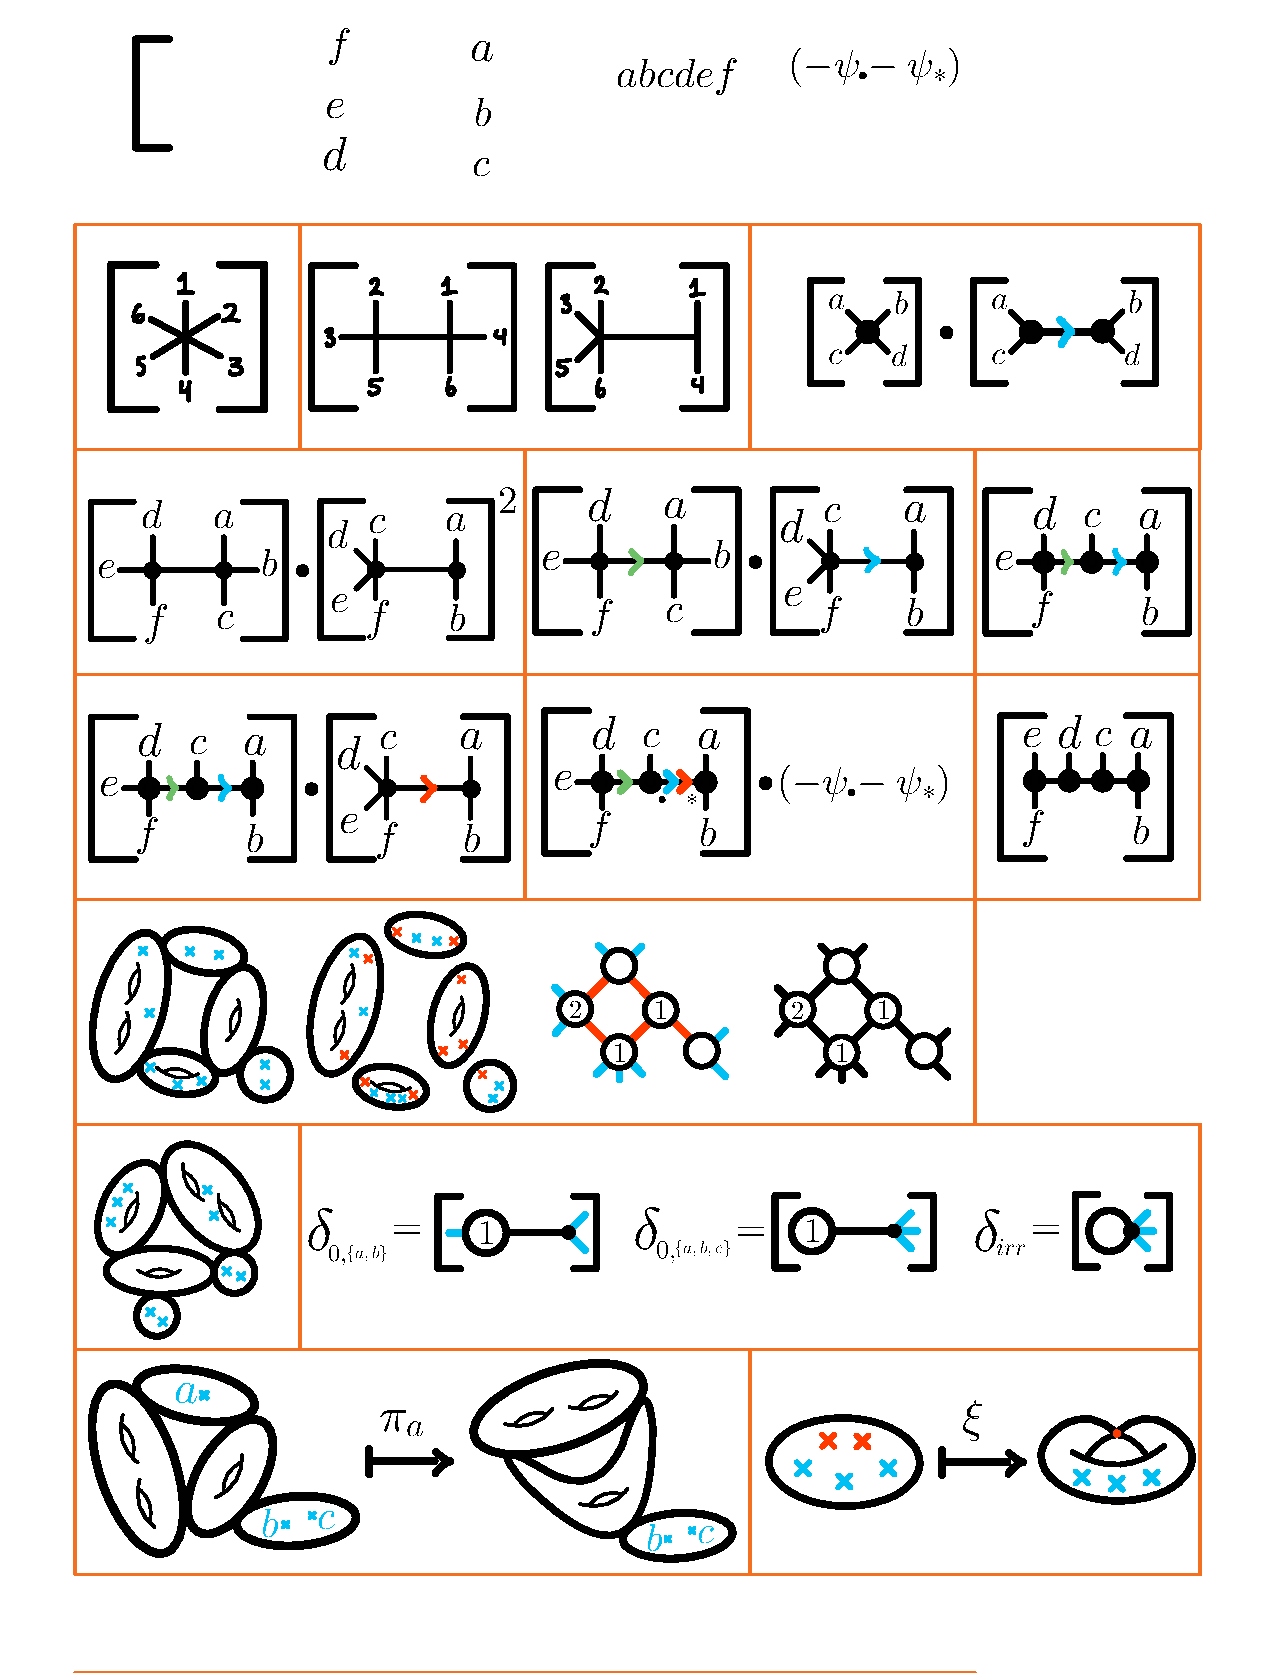
\includegraphics[width=0.2\textwidth, trim= 1.32cm 20.75cm 16.53cm 3.9cm,clip]{../figs/FigsDNnotability1.pdf}
        \caption{Fundamental class representative of $\ov{M}_{0,6}$}
        \label{fig:fundamental-class-M06}
    \end{figure} 
    The top stratum in $\ov M_{0,6}$ contains only one topological type of curve as all other $6$-pointed $\bP^1$'s will be homeomorphic to this one.
\end{Ex}

\begin{Ex}
    Going into the boundary of $\ov M_{0,6}$ we can find two different types of strata of the form $\dl_{0,A}$, for example
    \begin{figure}[h!]
        \centering
        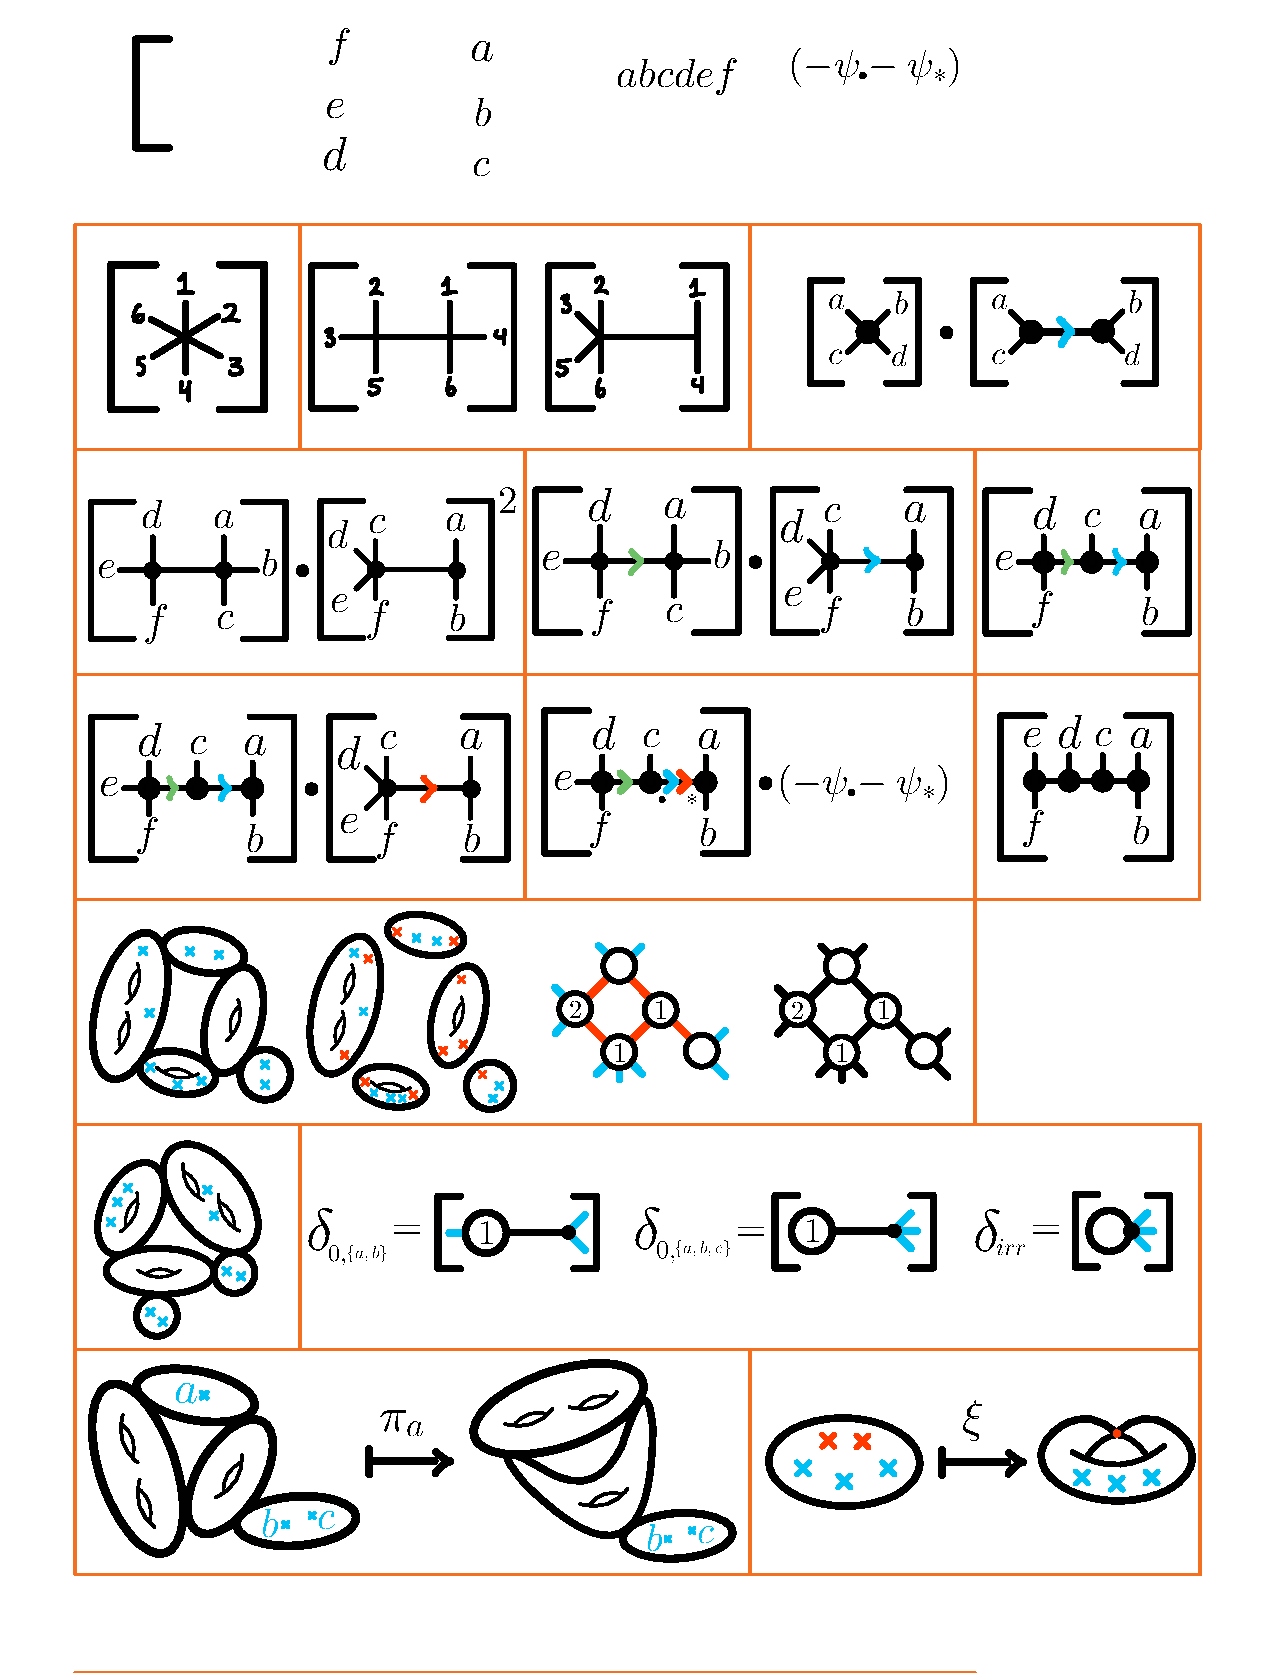
\includegraphics[width=0.4\textwidth, trim= 5.12cm 20.75cm 8.93cm 3.9cm,clip]{../figs/FigsDNnotability1.pdf}
        \caption{Boundary divisors $\dl_{0,\set{1,4,6}}$ and $\dl_{0,\set{1,4}}$ of $\ov{M}_{0,6}$}
        \label{fig:boundary-strata-M06c1}
    \end{figure} 
    From the stratum on the left, we can find $9$ other strata with the same graph design but different labelings. This is because there are 
    $$\half\binom{6}{3,3}=\frac{6!}{2\.3!\.3!}=10$$
    ways to label the tree. The factor of $\half$ accounts for the symmetry in the tree.\par
    For the one on the right we can find $\binom{6}{4,2}=15$ labelings. Observe that there is no class $\dl_{\text{irr}}$ in $\ov M_{0,6}$. 
\end{Ex}

In fact, there's not an irreducible divisor class until we start climbing up in genus. Before proceeding in this account, let's illustrate a bit of the combinatorics at hand. As we mentioned, the ability of representing a curve via a graph is of great help when enumerating this objects.

\begin{Prop}
    There are 
    $$\half\sum_{k=2}^{n-2}\binom{n}{k}=2^{n-1}-n-1$$
    irreducible boundary divisors in $\ov M_{0,n}$.
\end{Prop}

\begin{ptcbp}
    A partition into two sets of $\bonj{n}$ of size $k$ and $n-k$ can be done in $\binom{n}{k,n-k}$ ways. Observe that this coefficient is precisely $\binom{n}{k}$. We need to divide by 2 because $\binom{n}{k}=\binom{n}{n-k}$. And as we need $2\leq k\leq n-2$ for the curve to be stable, we must sum over all of those possibilities. 
\end{ptcbp}

\begin{Ex}
    Consider now the space $\ov M_{1,3}$ and let us identify the same kinds of classes here. The fundamental class can be immediately thought of as an elliptic curve with 3 marks. Up-to-topological type, there's two divisors of the form $\dl_{a,A}$. We have 
    $$\dl_{0,\set{a,b}},\word{and}\dl_{0,\set{a,b,c}}.$$ 
    These are represented by the graphs:
    \begin{figure}[h!]
        \centering
        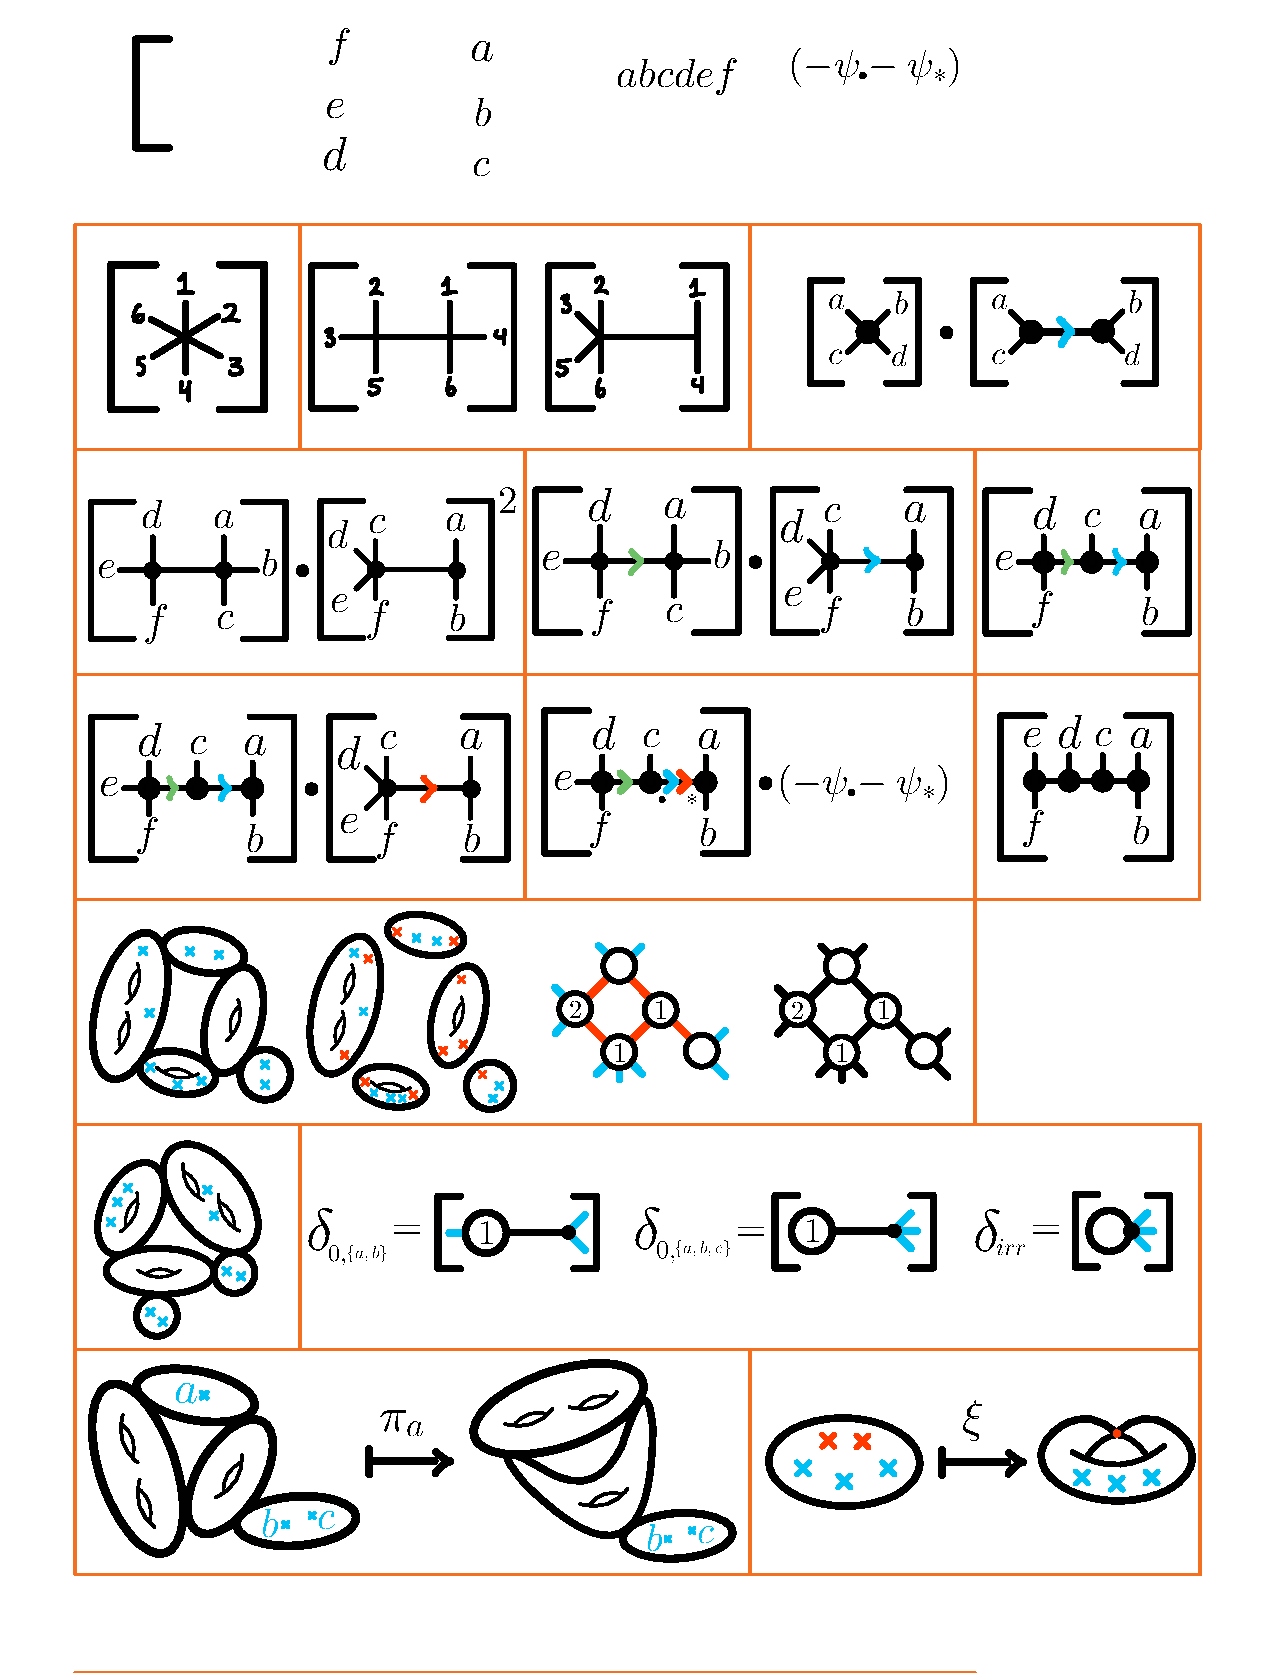
\includegraphics[width=0.8\textwidth, trim= 5.12cm 6.5cm 5.7cm 19.8cm,clip]{../figs/FigsDNnotability1.pdf}
        \caption{Boundary divisors $\dl_{0,\set{a,b}}$ and $\dl_{0,\set{a,b,c}}$ (marks unlabeled)}
        \label{fig:boundary-divs-M13c1}
    \end{figure}\par
    Whereas the irreducible divisor appears as follows: 
    \begin{figure}[h!]
        \centering
        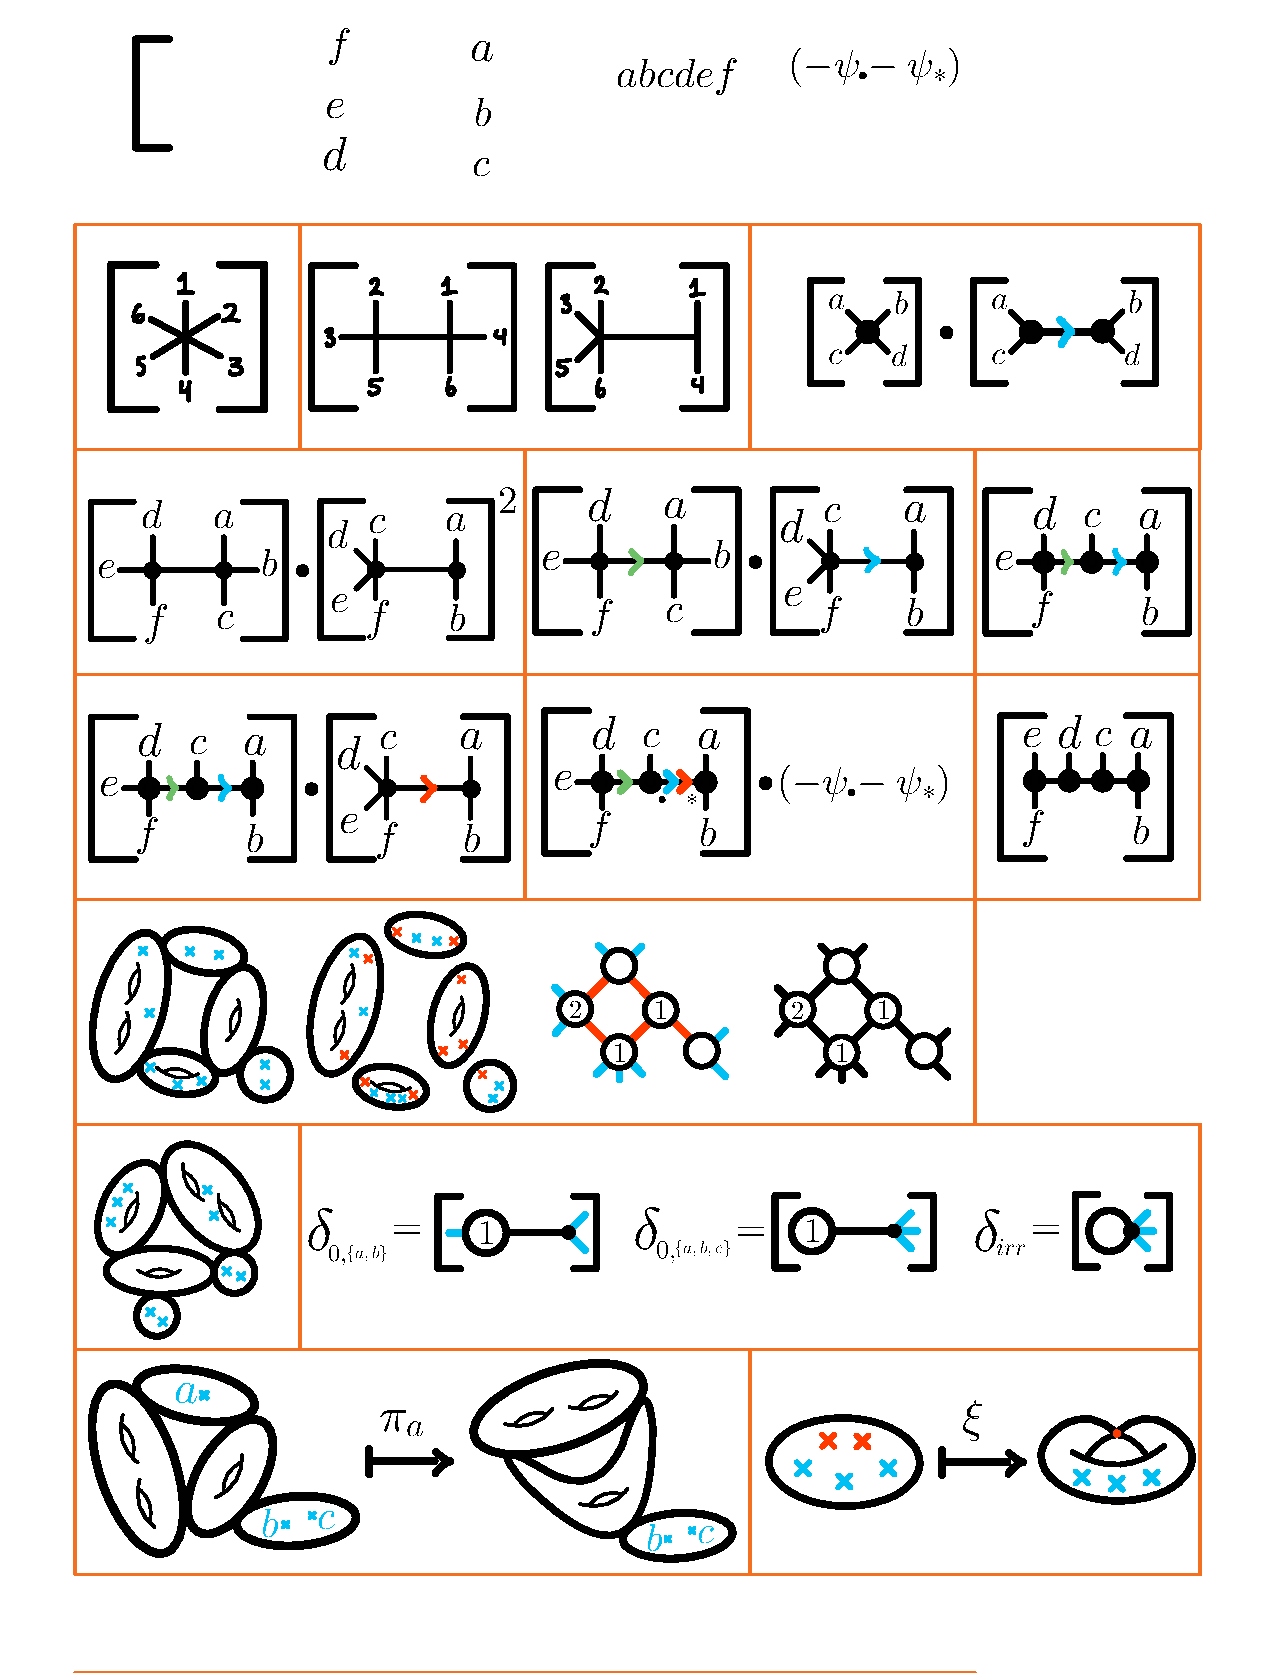
\includegraphics[width=0.3\textwidth, trim= 16.5cm 6.5cm 1.4cm 19.8cm,clip]{../figs/FigsDNnotability1.pdf}
        \caption{Irreducible boundary divisor in $\ov{M}_{1,3}$ (marks unlabeled)}
        \label{fig:boundary-irr-M13c1}
    \end{figure}
\end{Ex}

\begin{Rmk}
    Recall the example \ref{ex-Mg1n1-compactification} when we discussed which curve to add to compactify $M_{1,1}$. It is precisely the corresponding $\dl_{\text{irr}}$ the one which we added.
\end{Rmk}

We will restrict ourselves further inside the Chow ring of $\ov M_{g,n}$. 

\begin{Def}[\cite{ZvonkineIntro}, Def. 2.6]
The minimal family of subrings $R^\ast(\ov M_{g,n})\subseteq A^\ast(\ov M_{g,n})$ stable under pushforwards by forgetful and gluing maps is called the family of \term{tautological rings} of the moduli space of stable curves.
\end{Def}

Intuitively, the forgetting and gluing morphisms do what we expect them to do, they either ``forget'' a marked point or ``glue'' a couple of points together.  

\begin{Def}[\cite{ArbarelloCornalba}, pg. 3]
    The \term{forgetful map} is 
    $$\pi\:\ov M_{g,n+1}\to\ov M_{g,n}$$ 
    and it assigns to a curve $(C,p_1,\dots,p_{n+1})$ the \emph{stabilization} of the curve $(C,p_1,\dots,p_n)$. Whereas the \term{gluing map} comes in two flavors. A self-gluing 
    $$\xi\:\ov M_{g-1,n+2}\to\ov M_{g,n}$$
    which takes the $(C,p_1,\dots,p_{n+1},p_{n+2})$ into $(C,p_1,\dots,p_n)$ that has a node in the place where it identified $p_{n+1},p_{n+2}$. This adds to the curve one arithmetic genus.\par
    On the other hand, the map 
    $$\eta\:\ov M_{g_1,n_1+1}\x\ov M_{g_2,n_2+1}\to\ov M_{g_1+g_2,n_1+n_2}$$
    glues two curves $(C_k,p_1,\dots,p_{n_k+1})$ at the points $p_{n_1+1},p_{n_2+1}$ creating a nodal curve.
\end{Def}

\begin{Rmk}
    The forgetful map 
    $$\pi\:\ov M_{g,n+1}\to\ov M_{g,n}$$ 
    is also known as the \term{universal curve} over $\ov M_{g,n}$. It has $n$ sections $(\sg_i)_{i\in \bonj{n}}$. The image under the section $\sg_i$ of the curve $(C,p_1,\dots, p_n)$ attaches to $C$ a $\bP^1$ at $p_i$ and at $0\in\bP^1$ and relabels $1$ to $p_i$ and $\infty$ to $p_{n+1}$.
\end{Rmk}

\begin{Ex}
    The fundamental class of $\ov M_{g,n}$ is mapped via the section $\sg_i$ to the divisor $\dl_{0,\set{i,n+1}}$ for example.  
\end{Ex}

\begin{Rmk}
    Observe that when forgetting a mark in a $\bP^1$-tail with 2 marks we destabilize the curve as per the condition in theorem \ref{th-stability-condition-22gn}. This leads into a process called \term{stabilization}. This only occurs for $\bP^1$ components of our curve with less than three special points. The intuitive idea of what happens is that we collapse the component back into a point.
\end{Rmk}

\begin{Ex}
    Let's apply the forgetful map to a curve in $\ov M_{4,3}$ with marks $a,b$ and $c$. Applying $\pi_a$ leaves us with a destabilized $\bP^1$ component which contracts to a node joining the two components which it was connected to.
\begin{figure}[h!]
        \centering
        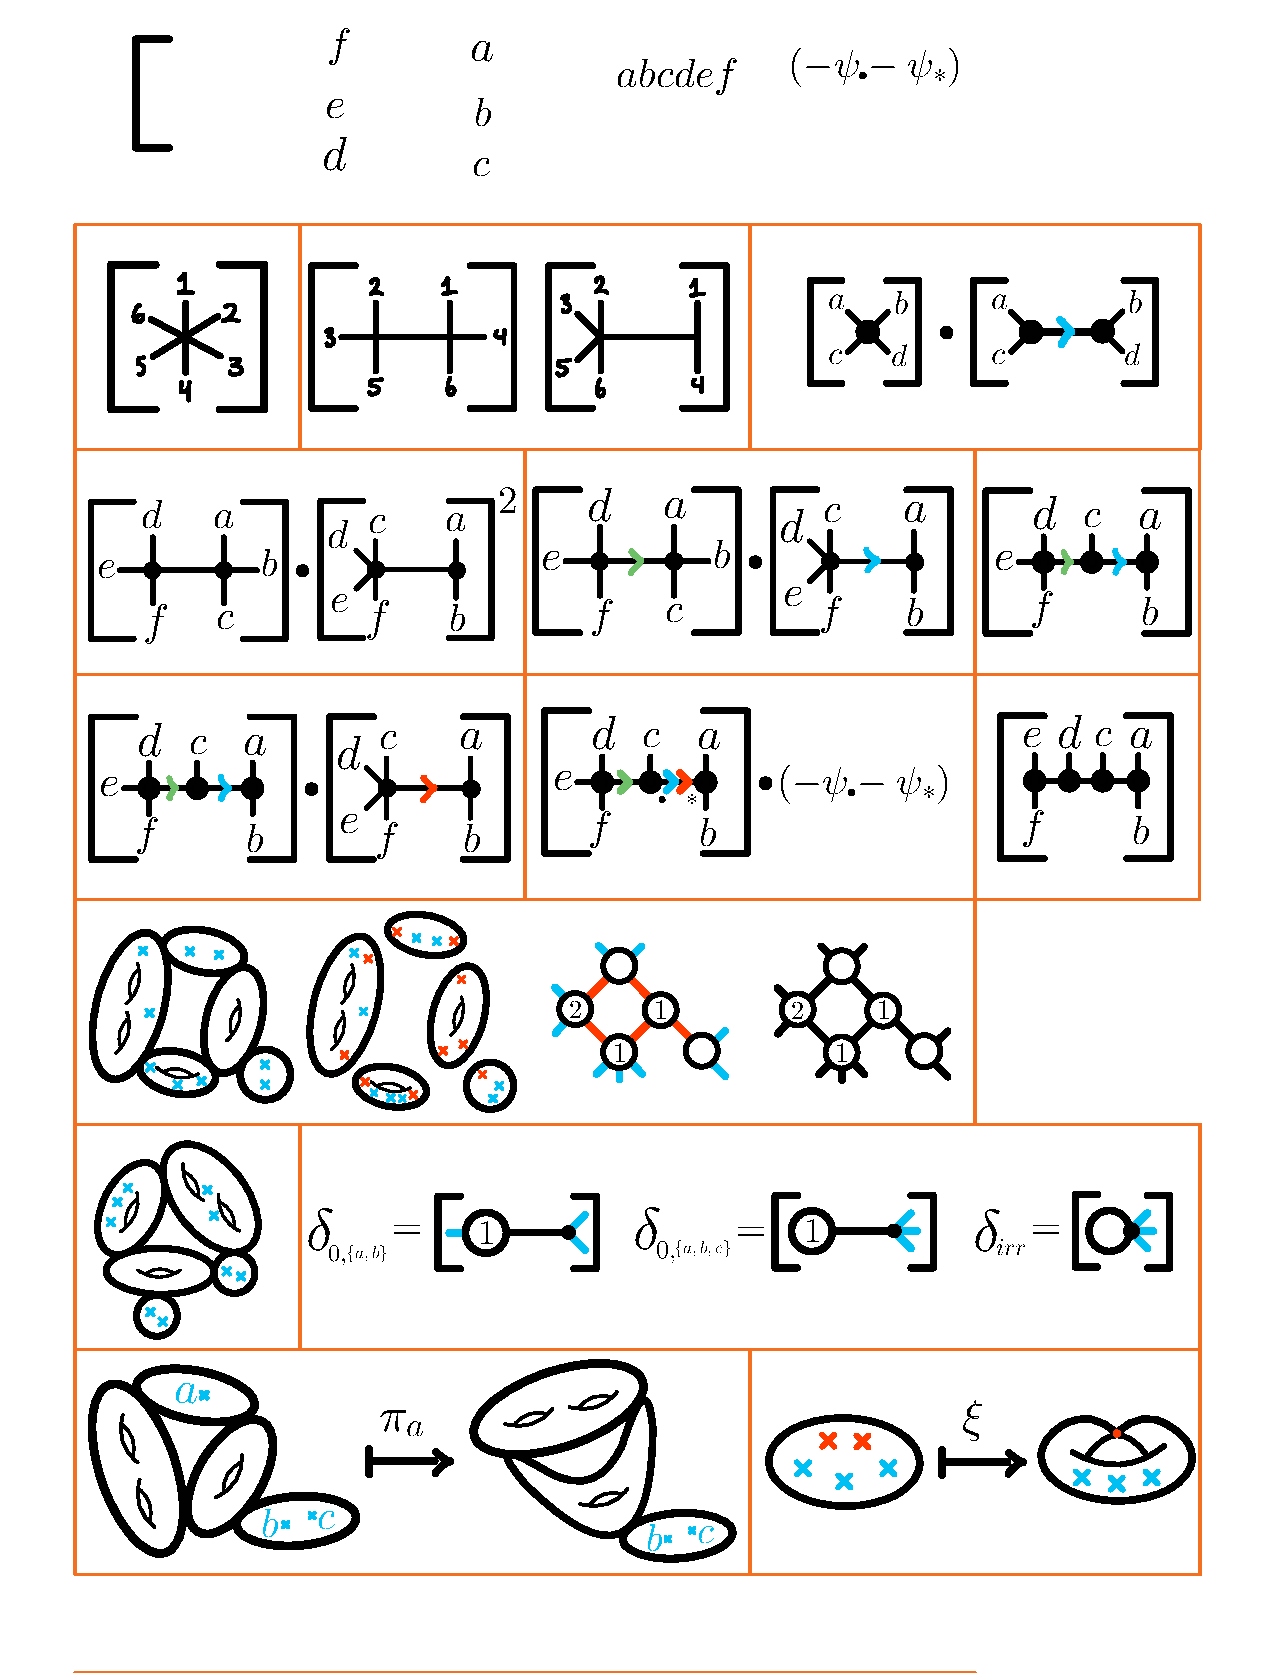
\includegraphics[width=0.8\textwidth, trim= 1.3cm 1.7cm 9cm 22.9cm,clip]{../figs/FigsDNnotability1.pdf}
        \caption{Marked curve in $\ov M_{4,3}$ and its stabilization after $\pi_a$}
        \label{fig:forget-mark-in-node}
    \end{figure}
On the other hand, if we forget the mark $b$, then the $\bP^1$ tail gets contracted into the node and the mark $c$ takes the place of the node.
\begin{figure}[h!]
        \centering
        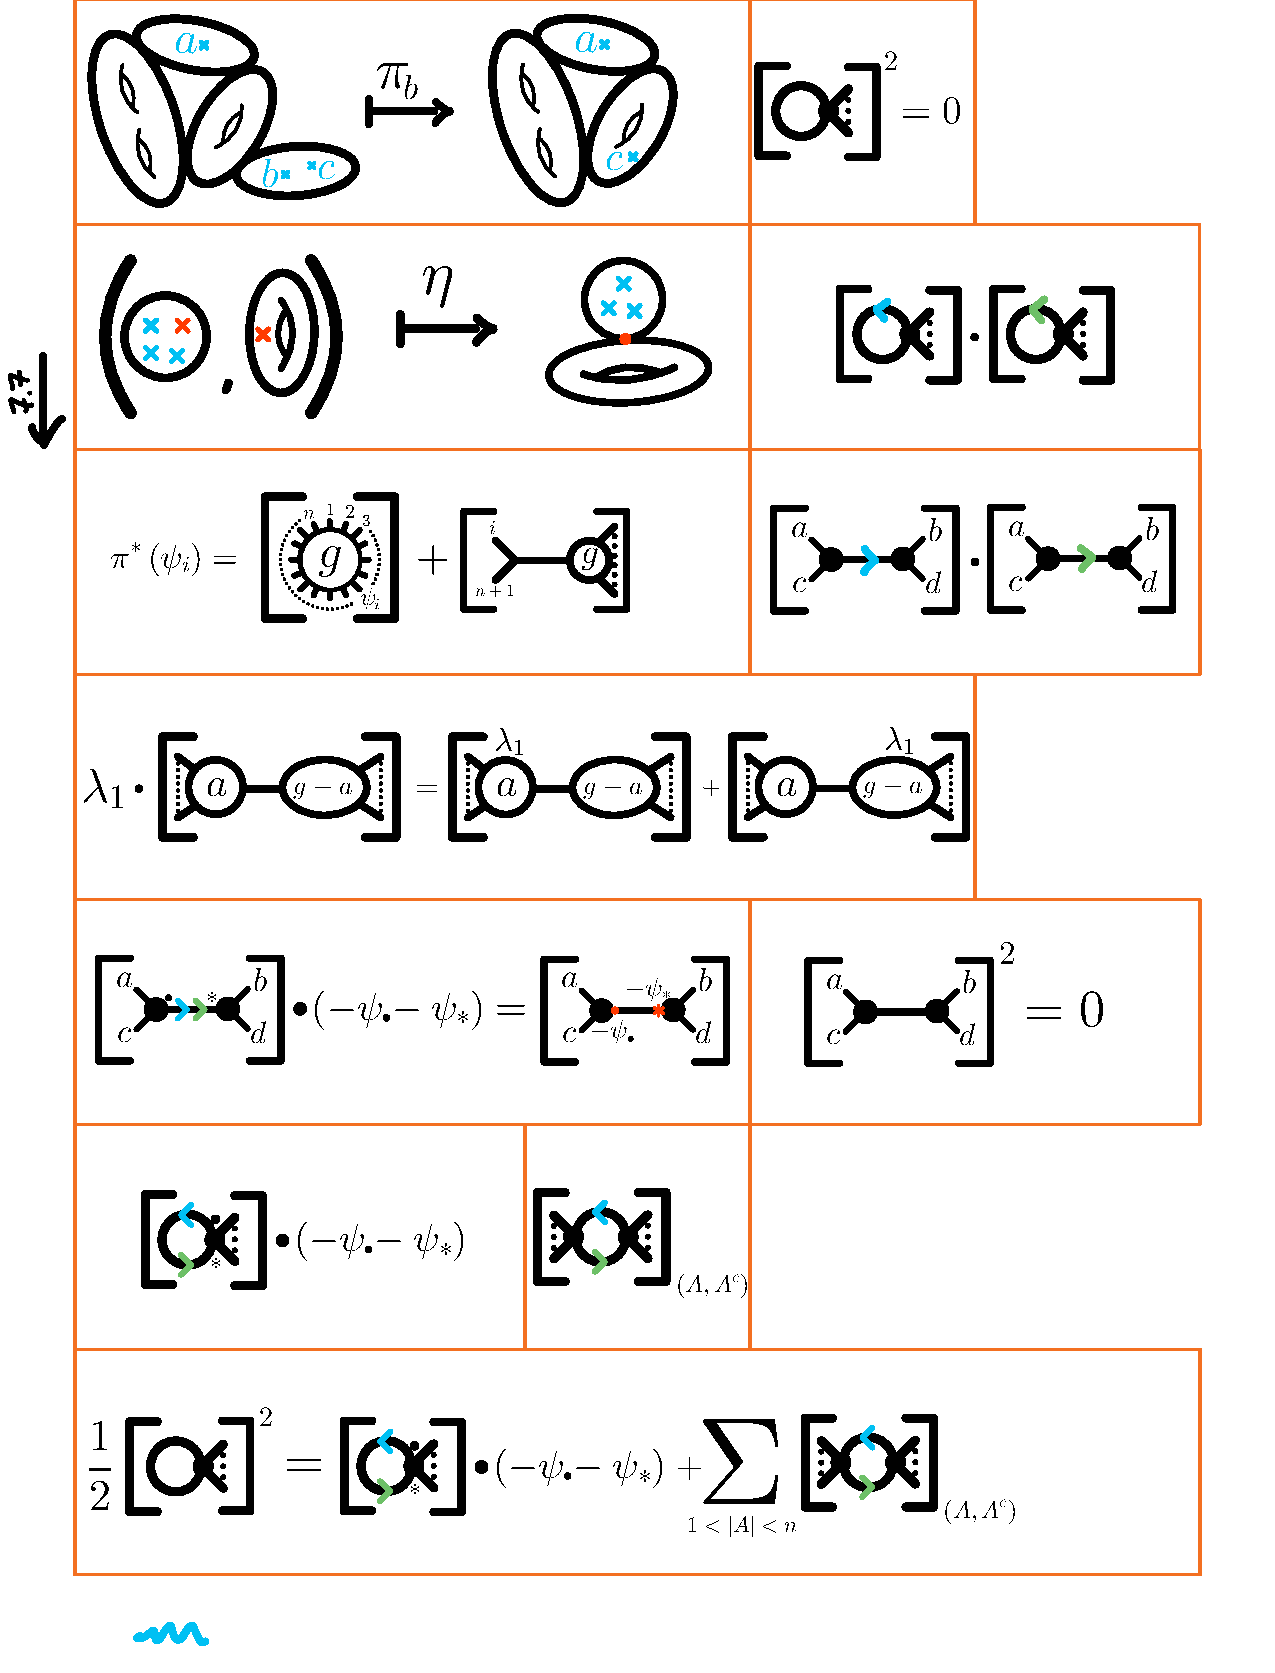
\includegraphics[width=0.8\textwidth, trim= 1.3cm 24.6cm 9cm 0.1cm,clip]{../figs/FigsDNnotability2.pdf}
        \caption{Same curve in $\ov M_{4,3}$ but stabilized after $\pi_b$}
        \label{fig:forget-mark-in-tail}
    \end{figure}
\end{Ex}

\begin{Rmk}
    One could think that an attached elliptic curve should get contracted as they have no visible marks, but they do have a special point, the node! It is in the case of pseudo-stable curves that we cannot have elliptic tails.
\end{Rmk}

Further information on stabilization can be found in \cite{GreenBookKockVainsencher} section 1.3 p. 23. But as long as we have the intuitive idea that components get contracted, we're good to go.

\begin{Ex}
    On the side of the self-gluing map observe that 
    $$\dl_{\text{irr}}=\half\xi_\ast 1.$$
    The half coefficient comes in for degree reasons, but intuitively this makes sense! We thus glue the fundamental class of $M_{0,5}$ to get $\dl_{\text{irr}}$ in $\ov M_{1,3}$.
    \begin{figure}[h!]
        \centering
        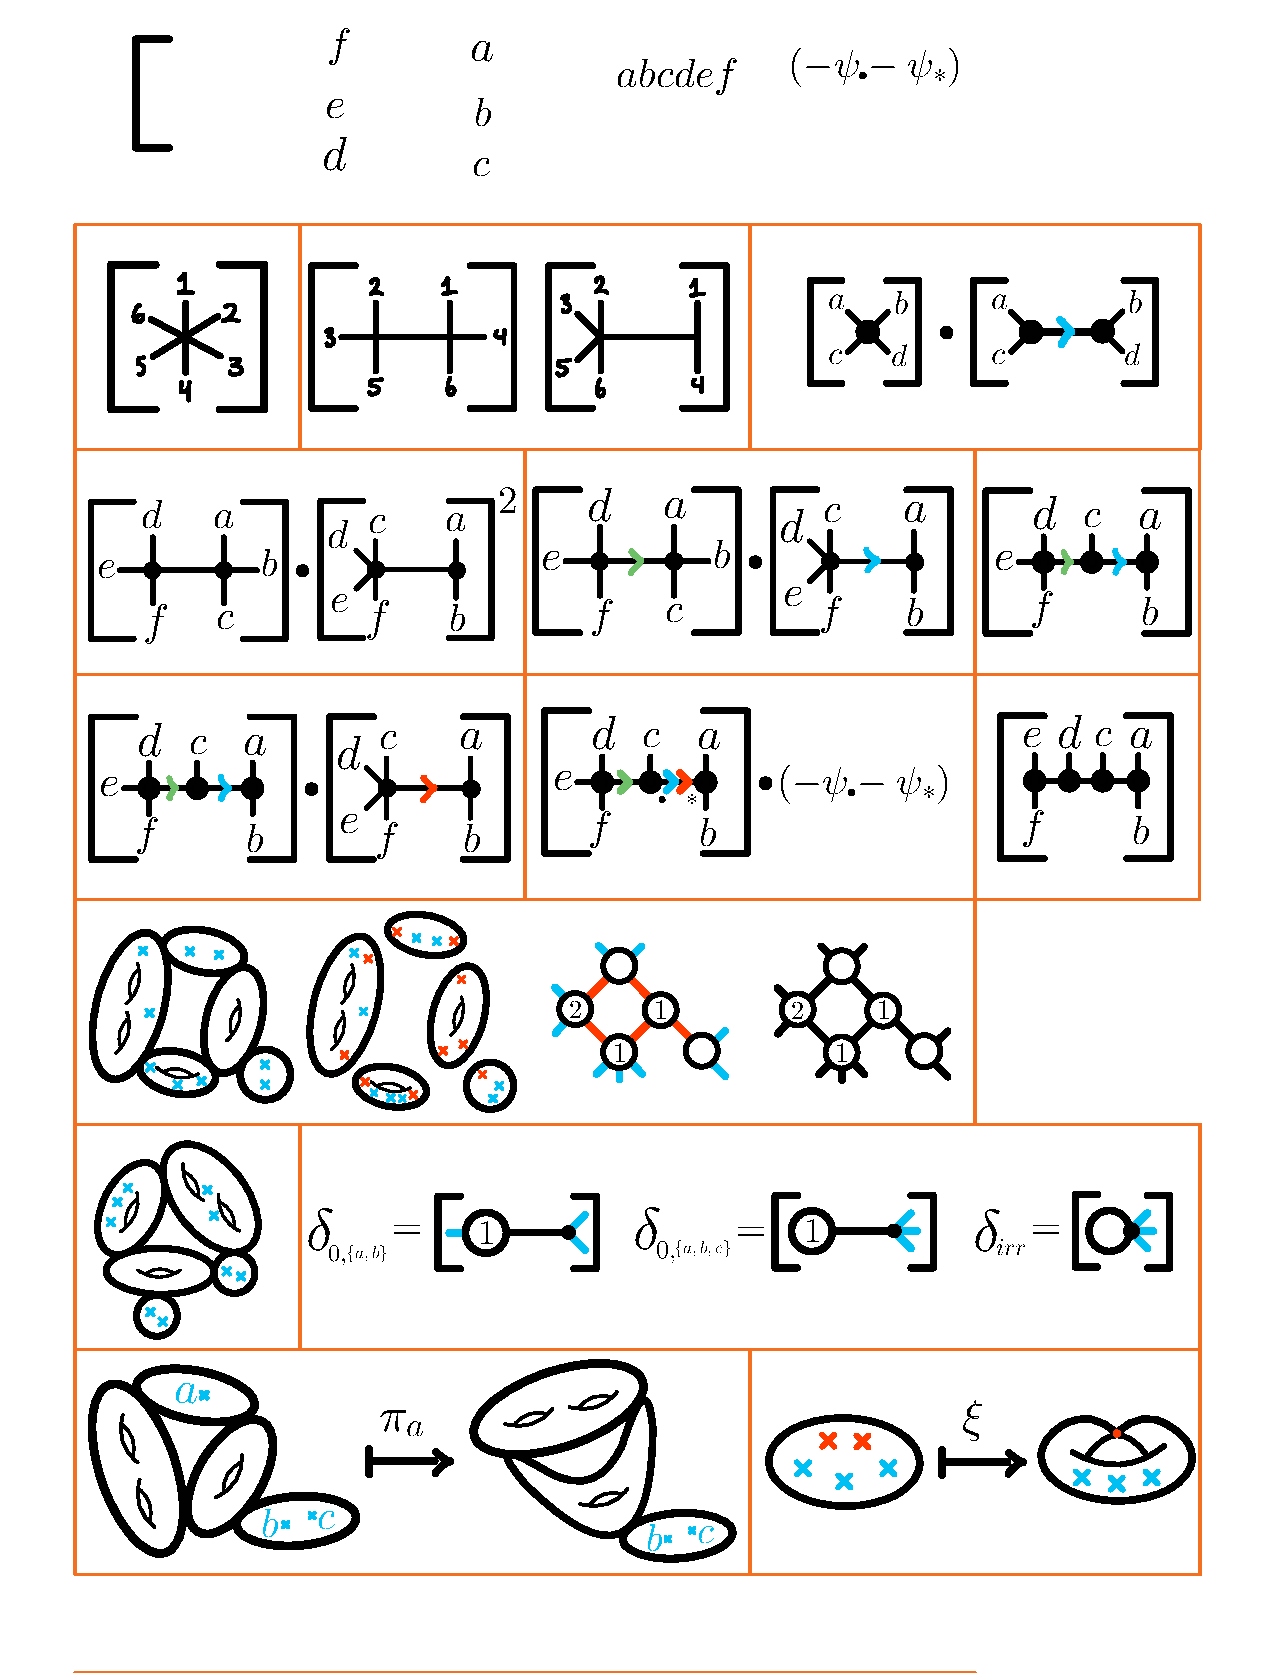
\includegraphics[width=0.6\textwidth, trim= 12.8cm 2.5cm 1.3cm 23.5cm,clip]{../figs/FigsDNnotability1.pdf}
        \caption{Gluing two red marks into a node}
        \label{fig:glue-fund05-irr13}
    \end{figure}
    The red point in the image is just to remind us that that is the point where the two original ones mapped to.
\end{Ex}

\begin{Ex}
    Finally consider gluing two different curves. The fundamental classes of $\ov{M}_{0,4}$ and $\ov{M}_{1,1}$.
    \begin{figure}[h!]
        \centering
        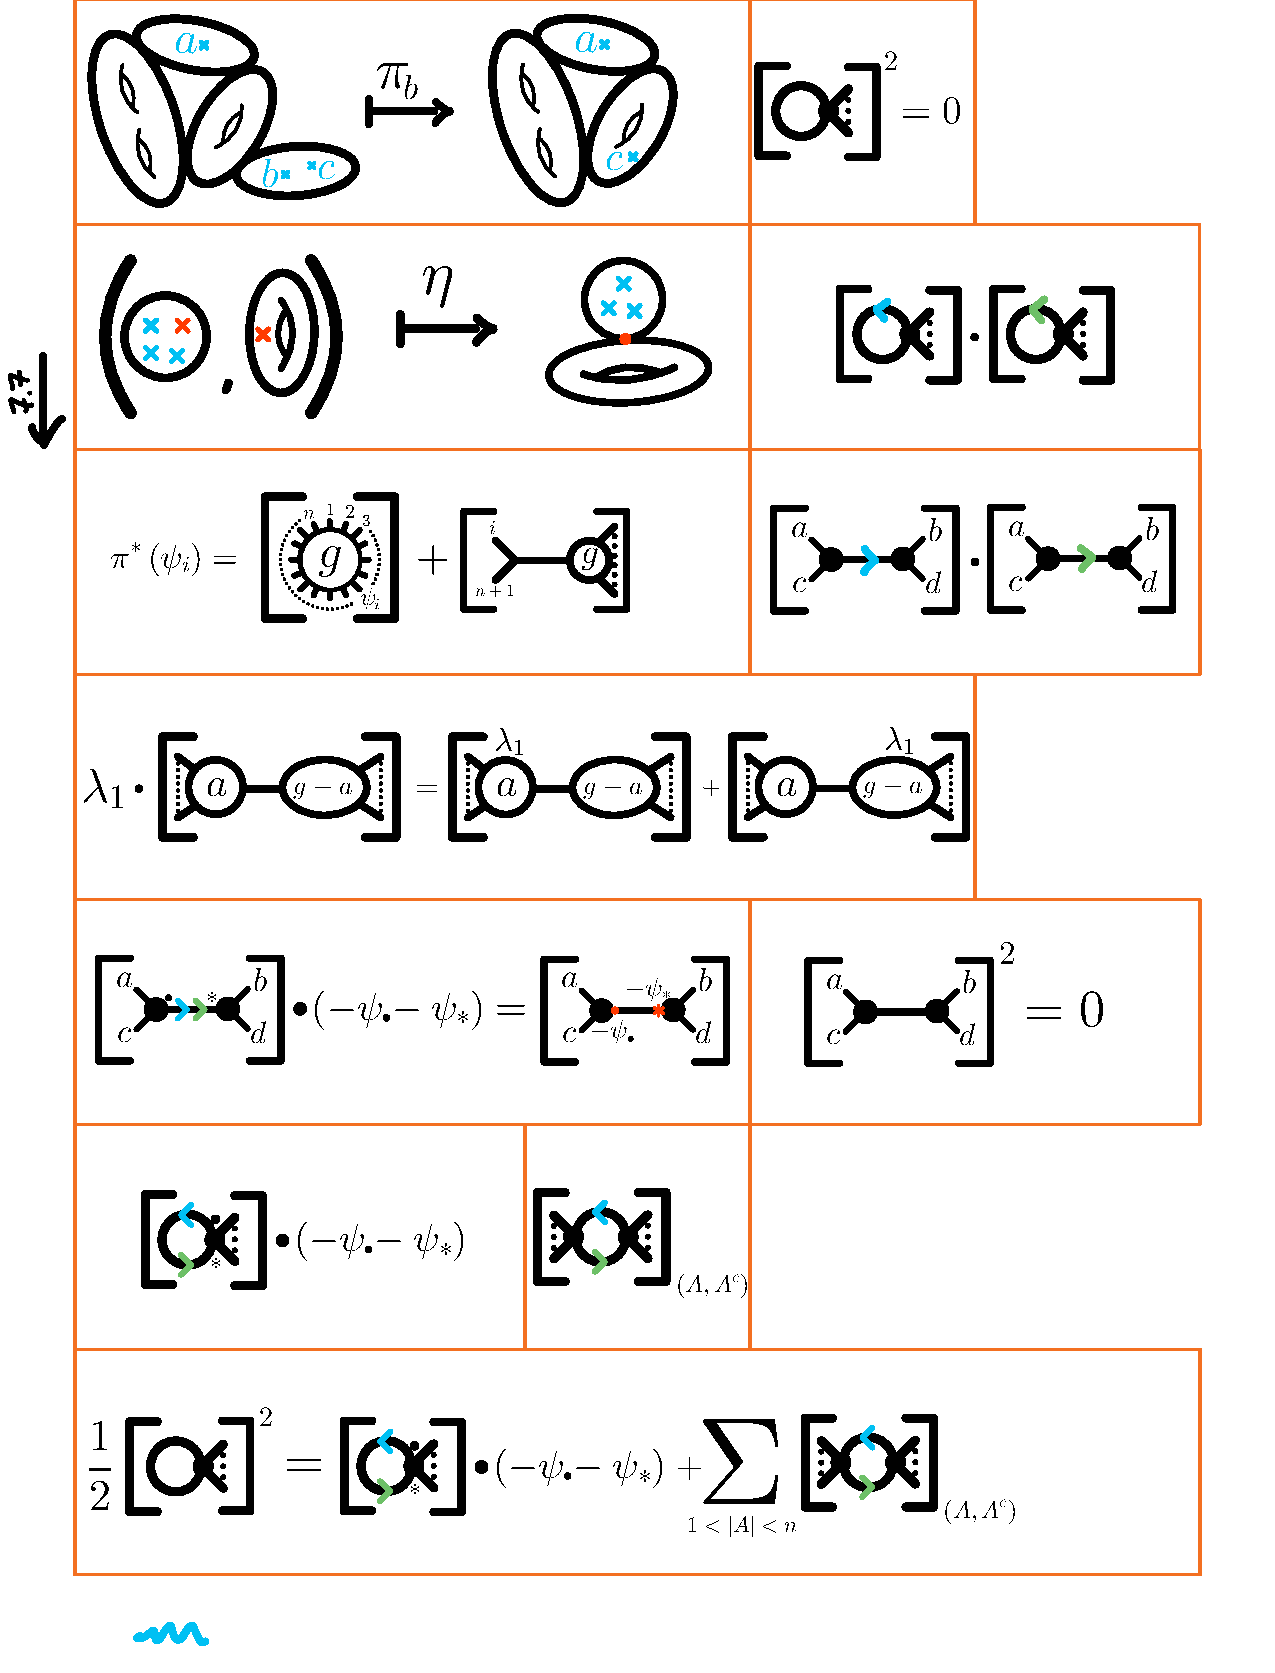
\includegraphics[width=0.7\textwidth, trim= 1.3cm 20.8cm 9cm 3.9cm,clip]{../figs/FigsDNnotability2.pdf}
        \caption{Gluing two curves into one}
        \label{fig:glue-two-into-divisor}
    \end{figure}
    Formally what we're doing here is 
    $$\eta(1,1)=\dl_{0,\set{a,b,c}}=\dl_{1,\emptyset}\in\ov{M}_{1,3}.$$
    Notice that both source curves had no codimension whereas the resulting one does have codimension!
\end{Ex}

\begin{Rmk}
    Both versions of the gluing map add one codimension because they're adding one node to a new curve.
\end{Rmk}

Now that we're equipped with this relatively intuitive classes we are ready to proceed into a bit more abstract classes of the moduli space.

\subsection{$\psi$ and $\lambda$ classes}

The quick reference for this part is \cite{cavalieri2022pseudostablehodgeintegrals} section 2.2. 

\begin{Def}
    The \term{cotangent line bundles} on $\ov M_{g,n}$ are defined by 
    $$\bL_i=\sg_i^\ast(\om_\pi)$$
    where $\om_\pi$ is the relative dualizing sheaf of the universal curve and $\sg_i$ is the section corresponding to the mark $p_i$. As the name suggests, the fiber of $\bL_i$ over $[(C,p_1,\dots,p_n)]$ is the cotangent line of $C$ at $p_i$.\par
    The $i^{\text{th}}$ \term{psi-class} $\psi_i$ is the first Chern class of $\bL_i$
    $$\psi_i=c_1(\bL_i)\in A^1(\ov M_{g,n})\word{for}i\in\bonj{n}.$$
\end{Def}

\begin{Def}
    The \term{Hodge bundle} on $\ov M_{g,n}$ is a rank $g$ vector bundle and is defined as 
    $$\bE=\pi_\ast(\om_\pi).$$
    Its fiber over a point $[(C,p_1,\dots,p_n)]$ is $\Ga(C,\om_C)$, the $g$-dimensional space of global sections of the dualizing sheaf of $C$.\par
    The $j^{\text{th}}$ \term{lambda-class} $\la_j$ is the $j^{\text{th}}$ Chern class of $\bE$
    $$\la_j=c_j(\bE)\in A^j(\ov M_{g,n})\word{for}j\in\bonj{g}.$$
\end{Def}

\begin{Rmk}
    Explaining a bit more on what the fibers of the Hodge bundle are, we have the following:
    \begin{itemize}
        \item For a smooth curve, it's holomorphic $1$-forms.
        \item When the curve is nodal, the fibers are $1$-forms at nodes such that the residues on both sides of the node are opposite. Recall that the residue theorem for complex surfaces states that sums of residues on both sides of a contour are equal.
    \end{itemize}
\end{Rmk}

Now returning to graphs, strata of $\ov M_{g,n}$ can support $\psi$ and $\la$ classes. In order to represent them in graphs we will add \emph{decorations}, $\psi$-classes on half-edges and $\la$ classes on vertices. 

\begin{Def}
    A \term{decorated stable graph} $\Ga$ is a stable graph $\un\Ga$ with the additional data of a monomial 
    $$\te_v=\prod_{i=1}^{n(v)}\psi^{e_i}_i\prod_{j=1}^{m}\la^{f_j}_j$$
    chosen for each vertex $v$.
\end{Def}

\begin{Ex}\label{ex-psi-class-forgetful-identity}
    In order to exemplify the decorated graphs, let's view a couple of formulae which will become useful the further we delve into this subject. If $\pi\:\ov M_{g,n+1}\to\ov M_{g,n}$ is the map which forgets $p_{n+1}$, then 
    $$\pi^\ast(\psi_i)=\psi_i-\dl_{0,\set{i,n+1}}\word{equivalently}\psi_i=\pi^\ast(\psi_i)+\Im\sg_i.$$
    Here the $\psi_i$ inside the pullback is supported on $\ov M_{g,n}$ whereas the other one in $\ov{M}_{g,n+1}$. Graphically this would be represented by two stable graphs, one decorated and the other one not.
    \begin{figure}[h!]
        \centering
        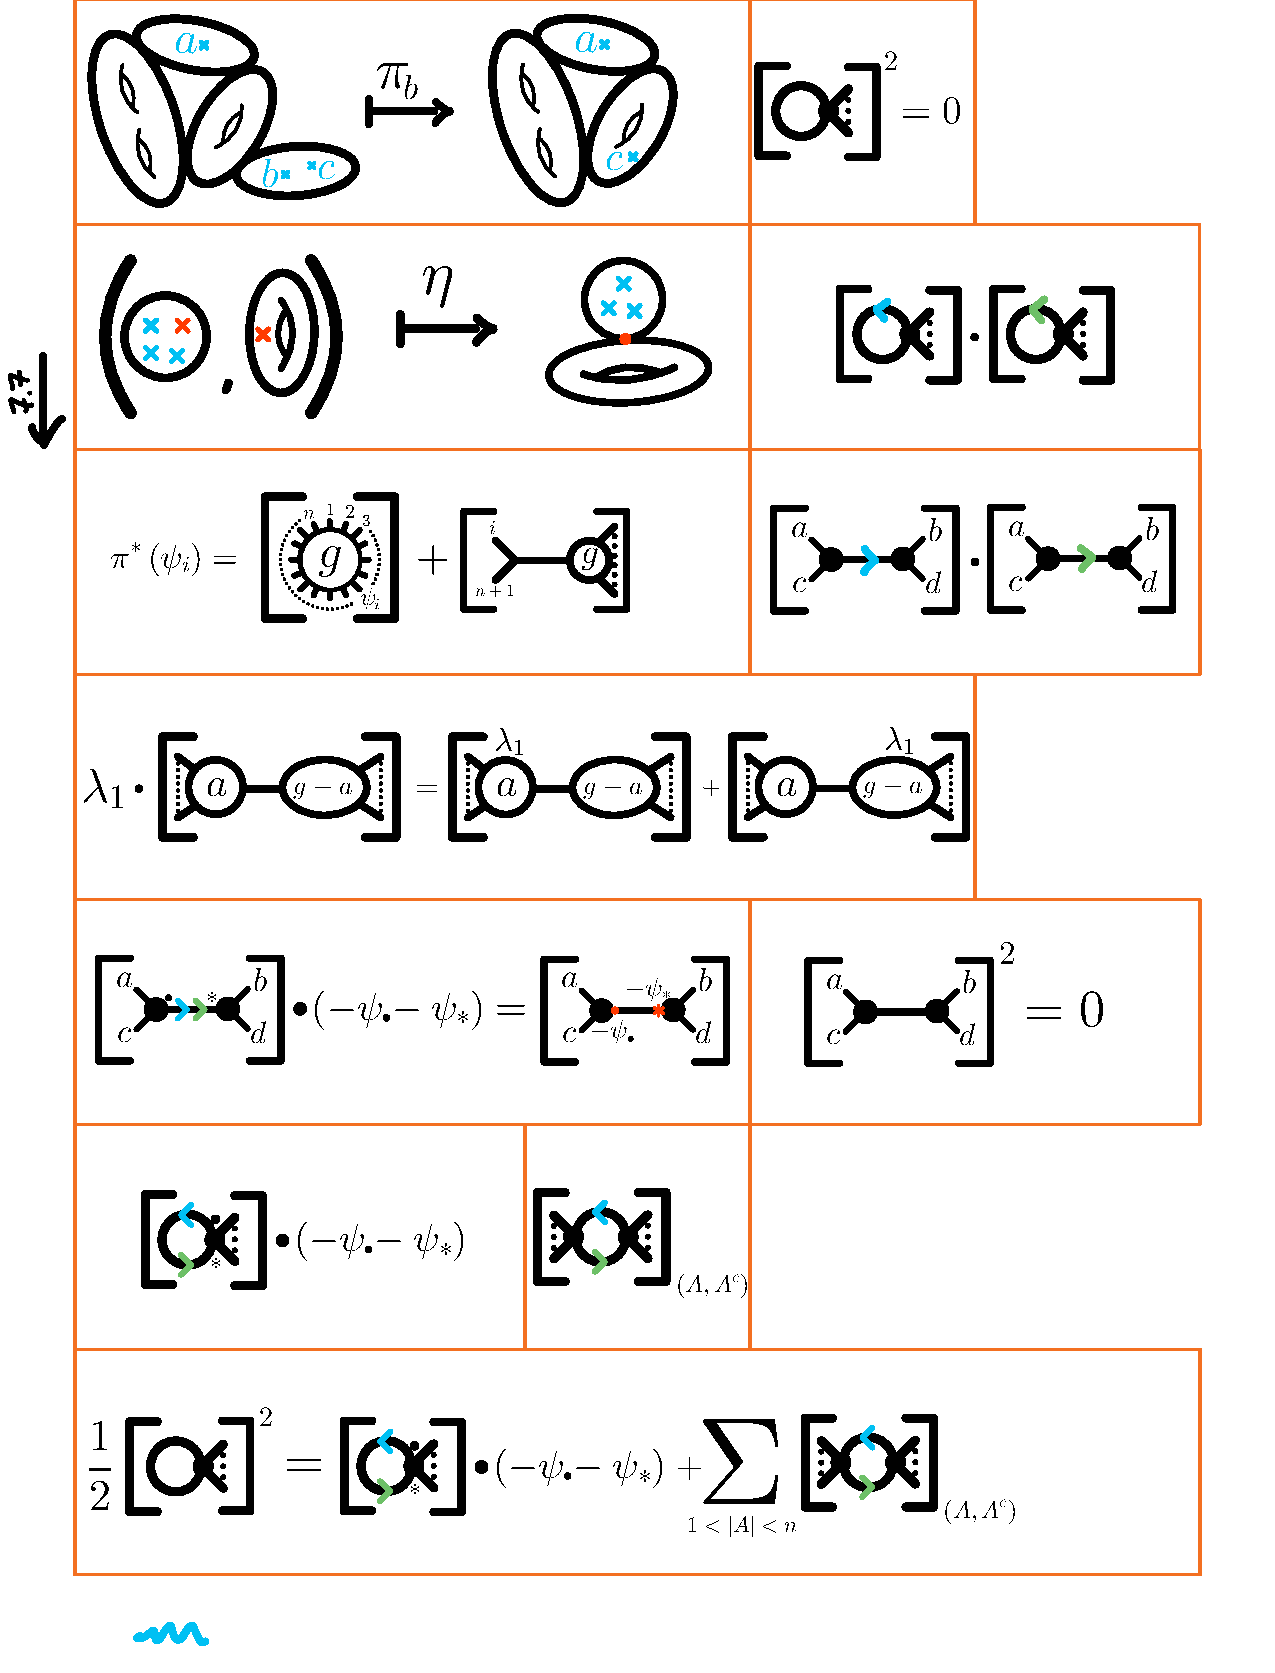
\includegraphics[width=0.7\textwidth, trim= 1.3cm 17cm 9cm 8cm,clip]{../figs/FigsDNnotability2.pdf}
        \caption{Psi-class forgetful formula}
        \label{fig:psi-class-forget}
    \end{figure}
\end{Ex}

From this we may extract a relation for psi-classes in $\ov{M}_{0,n}$ depending only on divisors of the form $\dl_{a,A}$.

\begin{Lem}[\cite{ArbarelloCornalba}, Prop. 1.6, pg. 5]\label{lem:divisor-sum-identity-psi-class}
    For any choice of marks $i,j,k$, arbitrary but fixed, the following relationship holds:
    $$\psi_i=\sum_{\substack{A\ni i\\ A\not\ni j,k}}\dl_{0,A}.$$
\end{Lem}

\begin{Ex}%https://mathoverflow.net/questions/100213/pull-back-of-hodge-bundle-via-glueing-map
    For lambda-classes, let's consider the Hodge bundle restricted to a divisor $\dl_{a,A}$ on $\ov M_{g,n}$. There exist projections 
    $$p_1\:\ov{M}_{g,n}\to\ov{M}_{a,|A|},\word{and}p_2\:\ov{M}_{g,n}\to\ov{M}_{g-a,n-|A|}$$
    through which we can pullback the Hodge bundles of the smaller moduli spaces and thus get 
    $$\left.\bE\right|_{\dl_{a,A}}=p_1^\ast\left(\bE_{a,|A|}\right)\oplus p_2^\ast\left(\bE_{g-a,n-|A|}\right).$$
    We can express this graphically for the first lambda-class.
     \begin{figure}[h!]
        \centering
        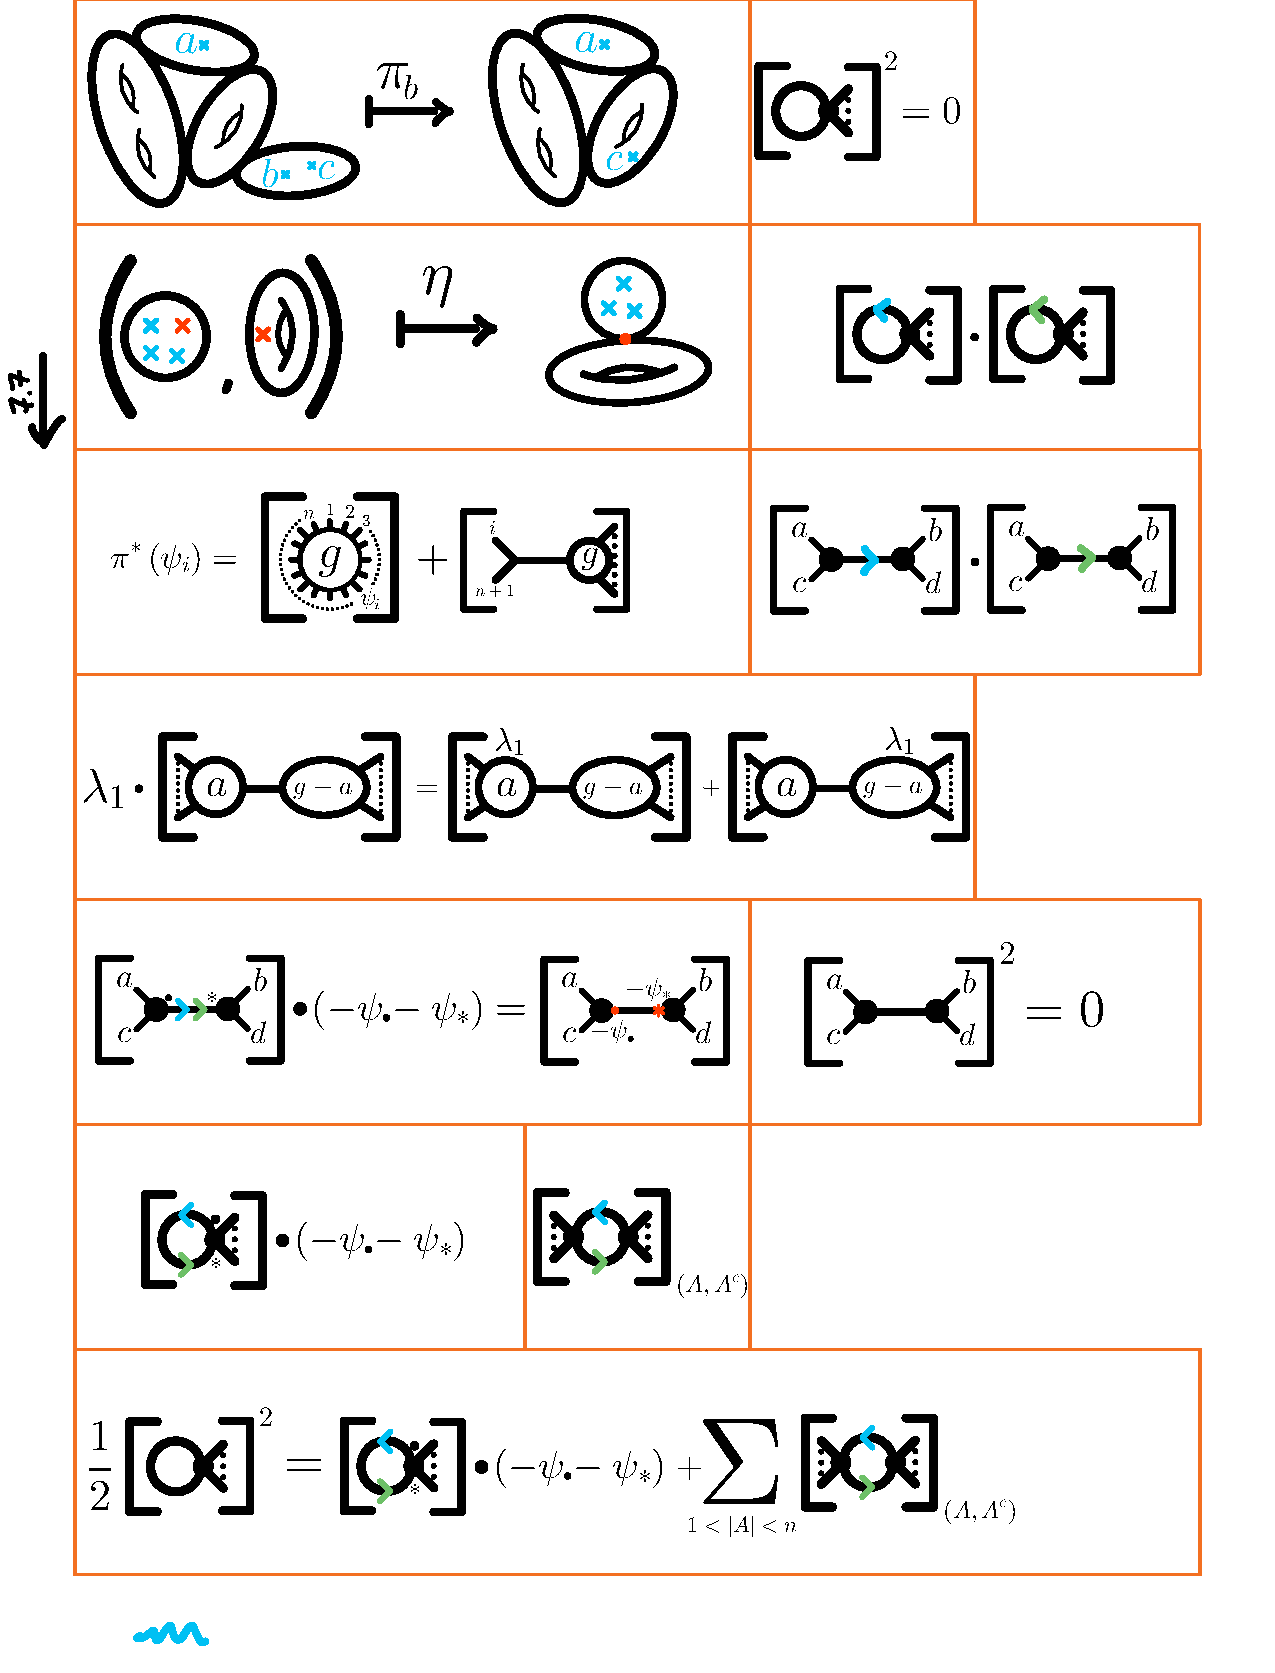
\includegraphics[width=0.8\textwidth, trim= 1.3cm 13.5cm 5.1cm 11.8cm,clip]{../figs/FigsDNnotability2.pdf}
        \caption{Lambda-class distribution}
        \label{fig:lambda-class-distribution}
    \end{figure}

    We haven't formally described how to compute the product of classes in $\ov M_{g,n}$ but this only requires knowing how to compute first Chern classes. Which we can do by using the cheat sheet theorem \ref{th-chern-class-cheat-sheet}.
\end{Ex}
As before, deep understanding or knowledge of what the relative dualizing sheaf is is not necessary to proceed. It's just important to know that these are special cohomology classes which show up when dealing with string theory as in the case of Witten's conjecture. More on psi-classes can be found in Zvonkine's article \cite{ZvonkineIntro} also in the viewpoint of differential forms which we don't touch here. Joachim Kock's notes on psi-classes \cite{KockPsiClasses} also contain valuable information. For now, let us put into practice the material which we've begun to describe. 

\section{The intersection product on $\ov M_{g,n}$}

As we have discussed before, the rich combinatorial structure of the cohomology classes allows us to enumerate properties of the curves we're talking about easily. The intersection of cohomology classes corresponds to the product in the Chow ring. So if we wish to enumerate properties of intersections, we must develop a way to multiply classes which respects the combinatorial structure.
 
\begin{Def}[\cite{SchmittVanZelm}, pg. 11]
Let $\Ga_1,\Ga_2$ be two stable graphs with the same set of legs $L$. A \term{$\Ga_2$-structure on $\Ga_1$} is a morphism
$$f\:\Ga_1\to\Ga_2,\quad f=(\al,\bt,\ga)$$
such that
$$\al\: V_1\onto V_2,\quad\bt\: H_2\hookto H_1,\quad\ga\: H_1\less\Im\bt\to V_2$$
satisfying
\begin{enumerate}
    \item the map $\bt$ commutes with involutions, i.e. $\bt\iota_2=\iota_1\bt$,
    \item the map $\al$ respects leg assignments, i.e. $\al\ze_1=\ze_2$,
    \item If $h\in H_1\less\Im\bt$ and $a_1(h)=v$ then $\al(v)=\ga(h)$, 
    \item and if $v\in V_2$, then 
    $$(\al^{-1}(v),\ga^{-1}(v),\bt(a^{-1}_2(v))\cup\ze_2^{-1}(v),g_1,\iota_1,a_1,\ze)$$
    is a stable graph of genus $g(v)$ where $g_1,a_1$ and $\iota_1$ are restricte to the appropriate subsets and $\ze$ is defined by $\ze_1$ on $\ze_2^{-1}(v)$ and by $a_1$ on $\bt(a^{-1}_2(v))$.
\end{enumerate}
When such a map exists, we can say either
\begin{itemize}
    \item $\Ga_1$ is a \term{specialization} of $\Ga_2$, or
    \item $\Ga_2$ is a \term{contraction} of $\Ga_1$.
\end{itemize}
\end{Def}

\begin{Rmk}
    In other words, when contracting $\Ga_1$ into $\Ga_2$, we are doing a similar process as to finding a minor $\Ga_1$ with extra steps.\par
    We can also extend the definition to say that $\widetilde{\Ga}$ has a $(\Ga_1,\dots,\Ga_n)$ structure whenever $\widetilde\Ga$ contracts into any of the $\Ga_i$.
\end{Rmk}

In order to multiply two classes via their graphs, we will look for graphs which contract into both factors of the product. 

\begin{Def}
    We call an $(A,B)$-structure on $\Ga$ a \term{generic structure} if every edge of $\Ga$ corresponds to an edge of $A$ or an edge of $B$. In other words if 
    $$\bt_A(H_A)\cup\bt_B(H_B)=H_\Ga.$$
    An $(A,B)$-edge will be an edge which is identified with both an edge of $A$ and one of $B$.
\end{Def}

Now we all the tools ready to define the multiplication of graphs which combinatorially explains multiplication of strata.

\begin{Def}[\cite{YangIntersections}, pg. 5]
    Let $G,H$ be decorated stable graphs and $\Ga(G,H)$ the set of graphs with generic $(G,H)$ structure. In other words, the set of all graphs which contract into $G$ and $H$ generically. Then the product of $G$ and $H$ is defined as 
    $$G\. H=\sum_{A\in\Ga(\un G,\un H)}\frac{1}{|\Aut(A)|}F_A(G,H)\.A$$
    where we have 
    $$
    \left\lbrace
    \begin{aligned}
        &F_A(G,H)=\left(\sum_{v\in V_G}f_A(G,v)\right)\left(\sum_{v\in V_H}f_A(H,v)\right)\prod_{e=(h_1,h_2)}(-\psi_{h_1}-\psi_{h_2})\\
        &f_A(G,v)=\prod_{i=1}^{n}\psi_{\bt(i)}^{e_i}\left(\sum_{w\in\al^{-1}(v)}\la_{j_w}\right)^{f_j}
    \end{aligned}
    \right.
    $$
    and the last product of $F$ is taken through the edges identified with both an edge of $G$ and an edge of $H$.
\end{Def}

As before, definitions come to life via examples. 

\begin{Ex}
    Let's begin with a sanity check. Consider the product in $\ov M_{0,4}$ of the fundamental class $1$ with $\dl_{0,{ac}}$. 
    \begin{figure}[h!]
        \centering
        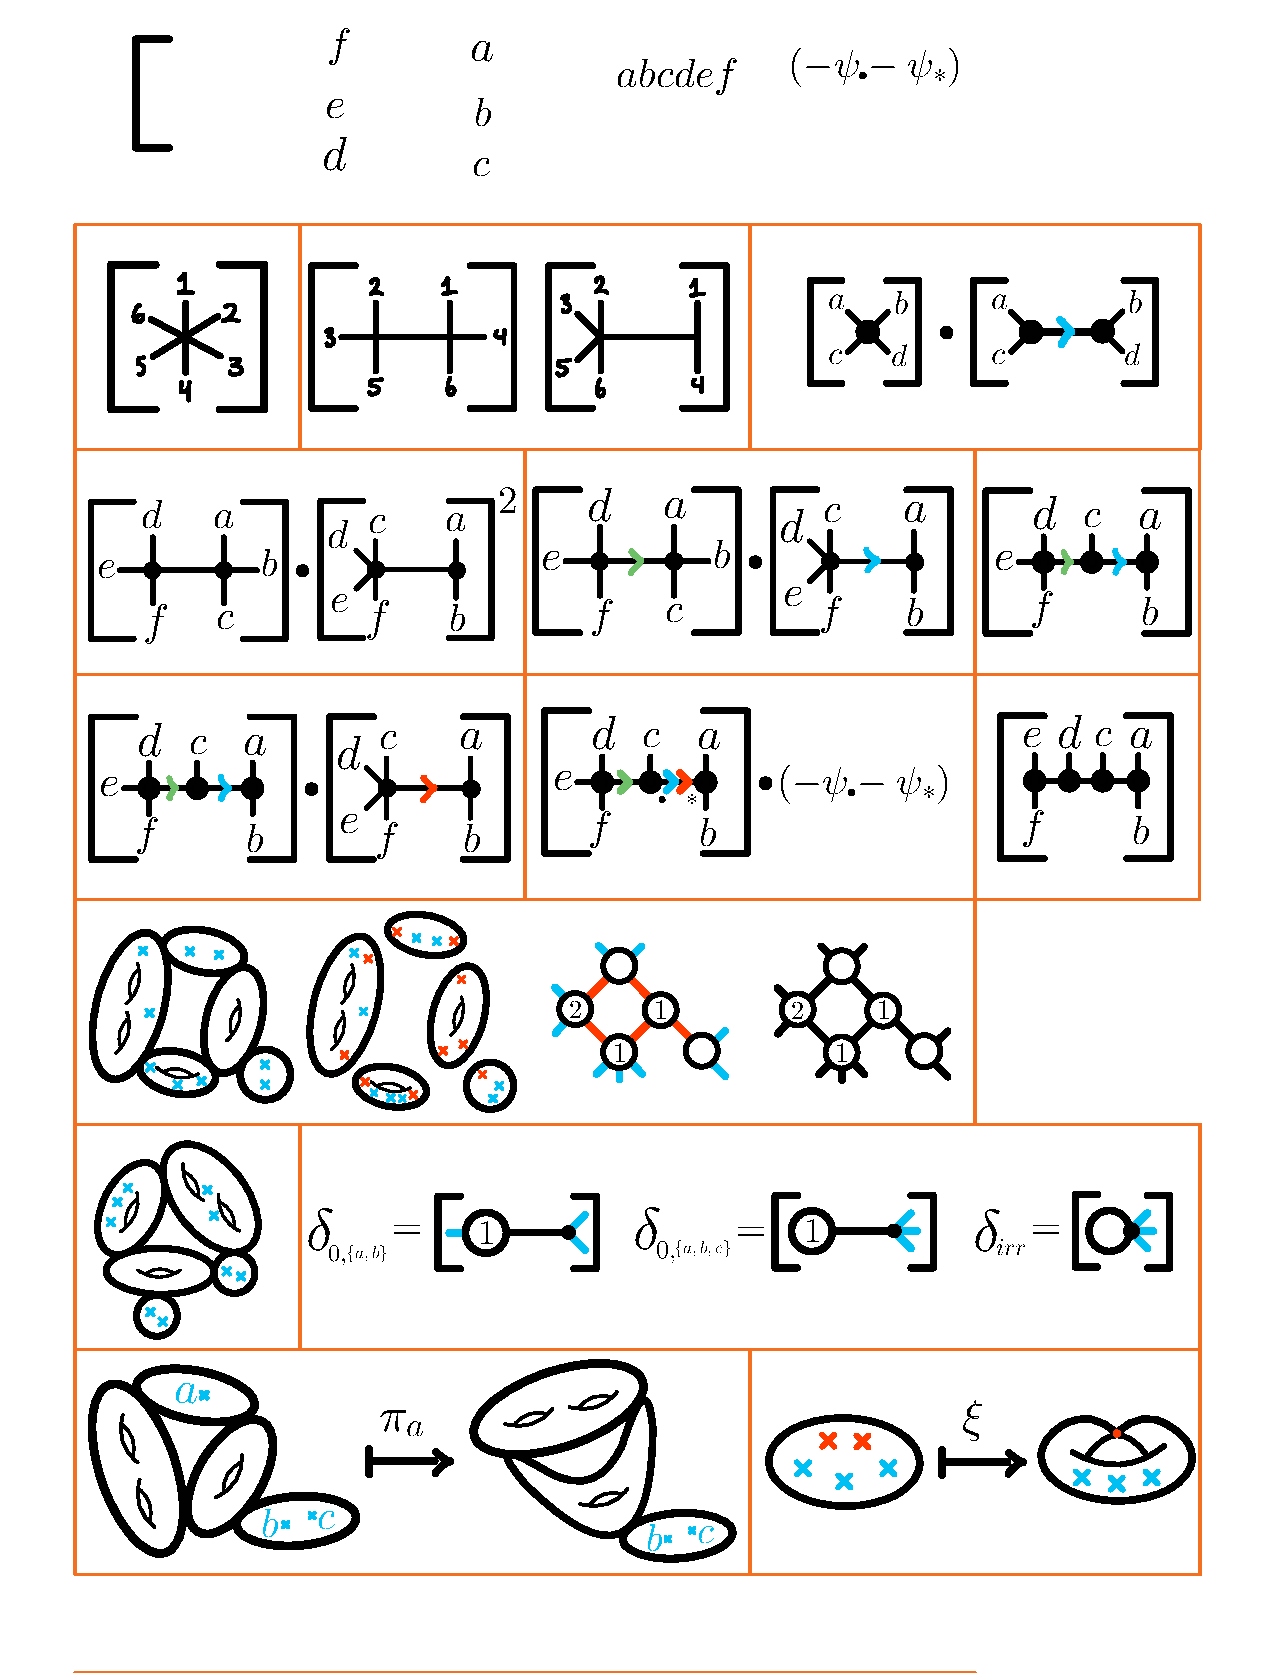
\includegraphics[width=0.5\textwidth, trim= 13cm 21.5cm 1.5cm 4.5cm,clip]{../figs/FigsDNnotability1.pdf}
        \caption{Trivial multiplication in $\ov M_{0,4}$}
        \label{fig:trivial-multiplication-M04}
    \end{figure} 
    Let's proceed by following the formula.
    \begin{enumerate}
        \item We have found the graphs representing the classes in question and now we look for graphs which generically contract into both of the factors. Observe that only $\dl_{0,{ac}}$ contracts into both itself and the fundamental class.
        \item The edge of $\dl_{0,{ac}}$ is colored so that we can look at which edges get identified with it when contracting. As there's no edge in $1$, the last product is empty.
        \item As there's no psi- nor lambda-classes, $f_A$'s are also trivial.
        \item Lastly, the graph $\dl_{0,{ac}}$ has no non-trivial automorphisms.
    \end{enumerate}
    Therefore it happens that:
    $$1\.\dl_{0,{ac}}=\left(1\.1\.\dl_{0,{ac}}\right)=\dl_{0,{ac}}$$
    as expected.
\end{Ex}

\begin{Rmk}
    Recall that the intersection product adds the codimensions of the factors. As $1$ has codimension $0$ and $\dl_{0,{ac}}$ has codimension 1, thus the result should have codimension $1$.\par
    Observe that this means that the resulting graphs can't have more edges than the total number edges in the factors, in this case they would also be non-generic!\par
    Another observation is that the graphs can indeed have less edges than the expected codimension. This is because we can have multiples of psi- and lambda-classes to even out the codimension.
\end{Rmk}

\begin{Ex}
    \begin{figure}[h!]
        \centering
        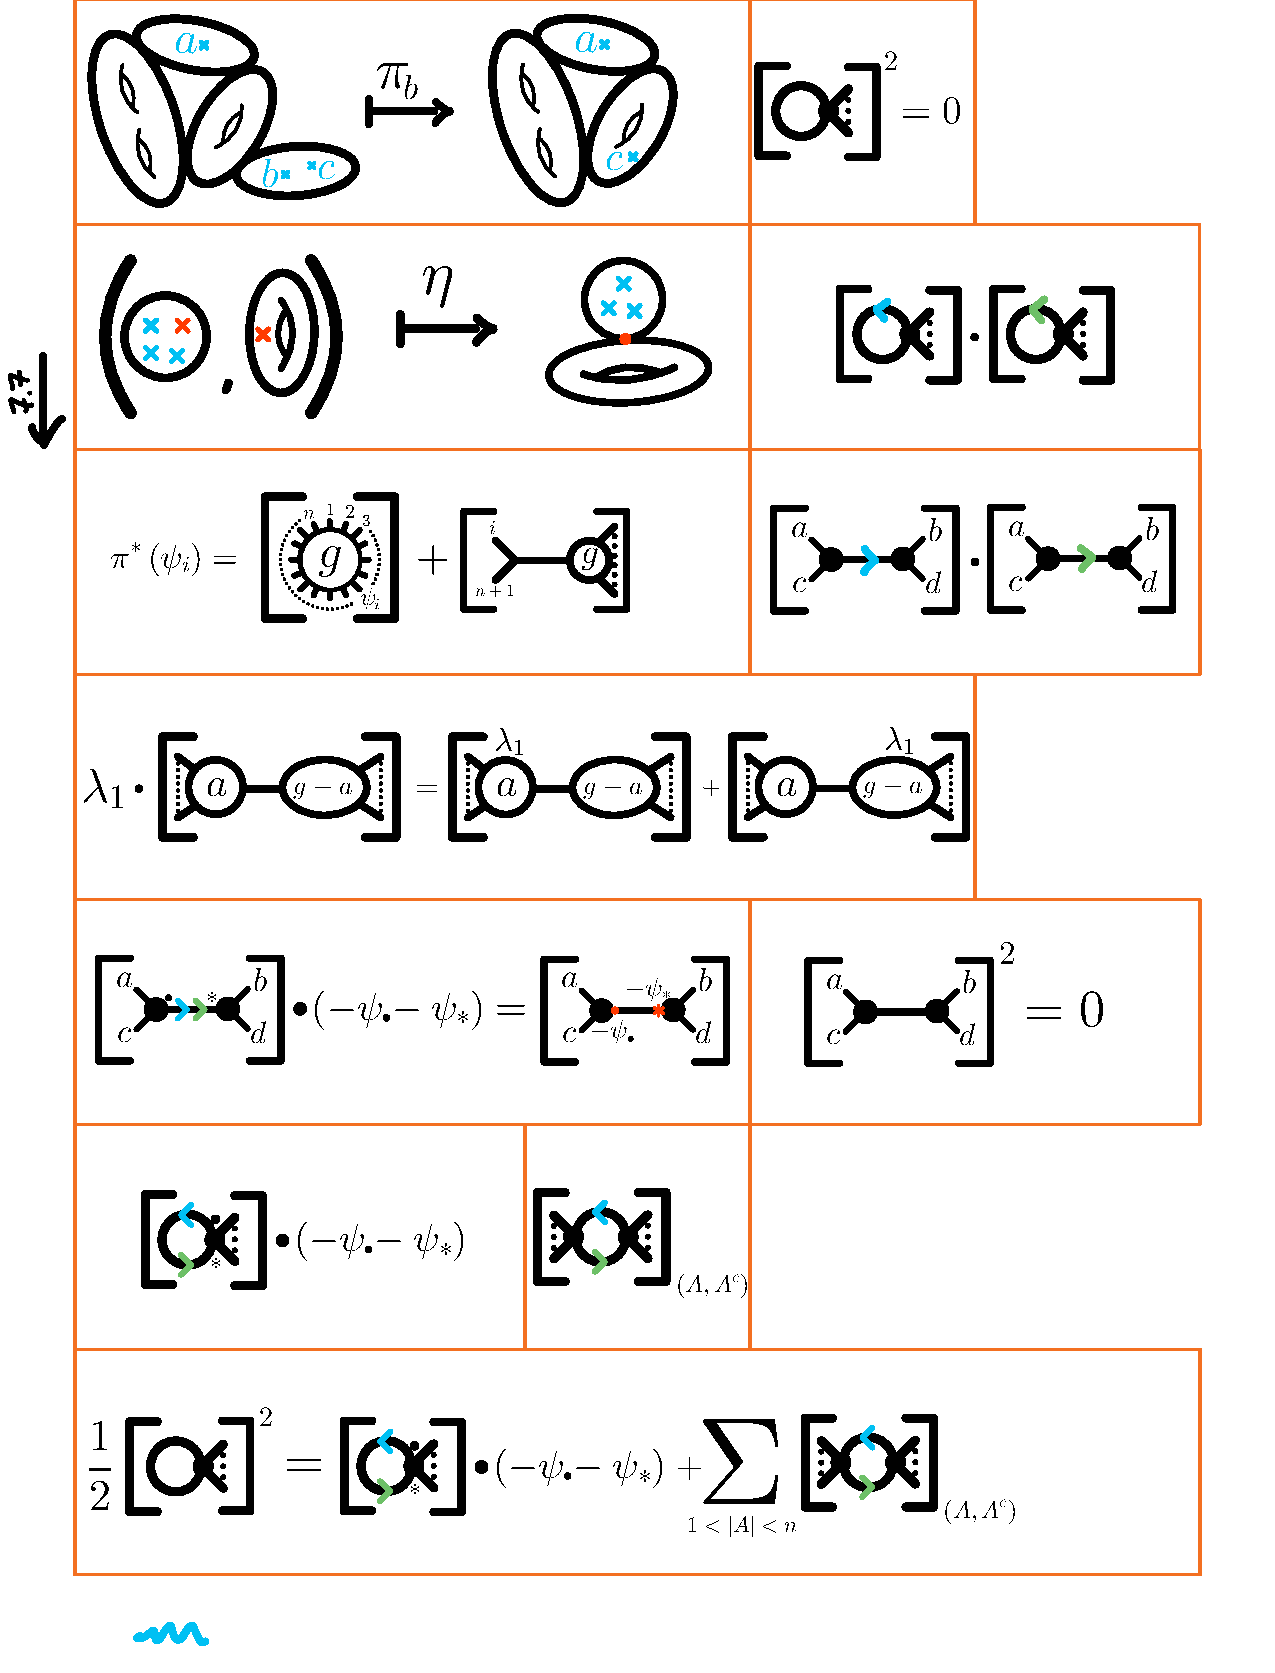
\includegraphics[width=0.5\textwidth, trim= 13cm 9.8cm 2cm 15.8cm,clip]{../figs/FigsDNnotability2.pdf}
        \caption{Divisor squared in $\ov M_{0,4}$}
        \label{fig:divisor-squared-M04}
    \end{figure} 
    Consider now the product $\dl_{0,{ac}}^2$ in $\ov{M}_{0,4}$. As this boundary divisor has codimension $1$, its square should have codimension $2$. As $\ov{M}_{0,4}$ has only one dimension, we expect the product to be empty. The edges of the factors are painted to distinguish them.
    \begin{figure}[h!]
        \centering
        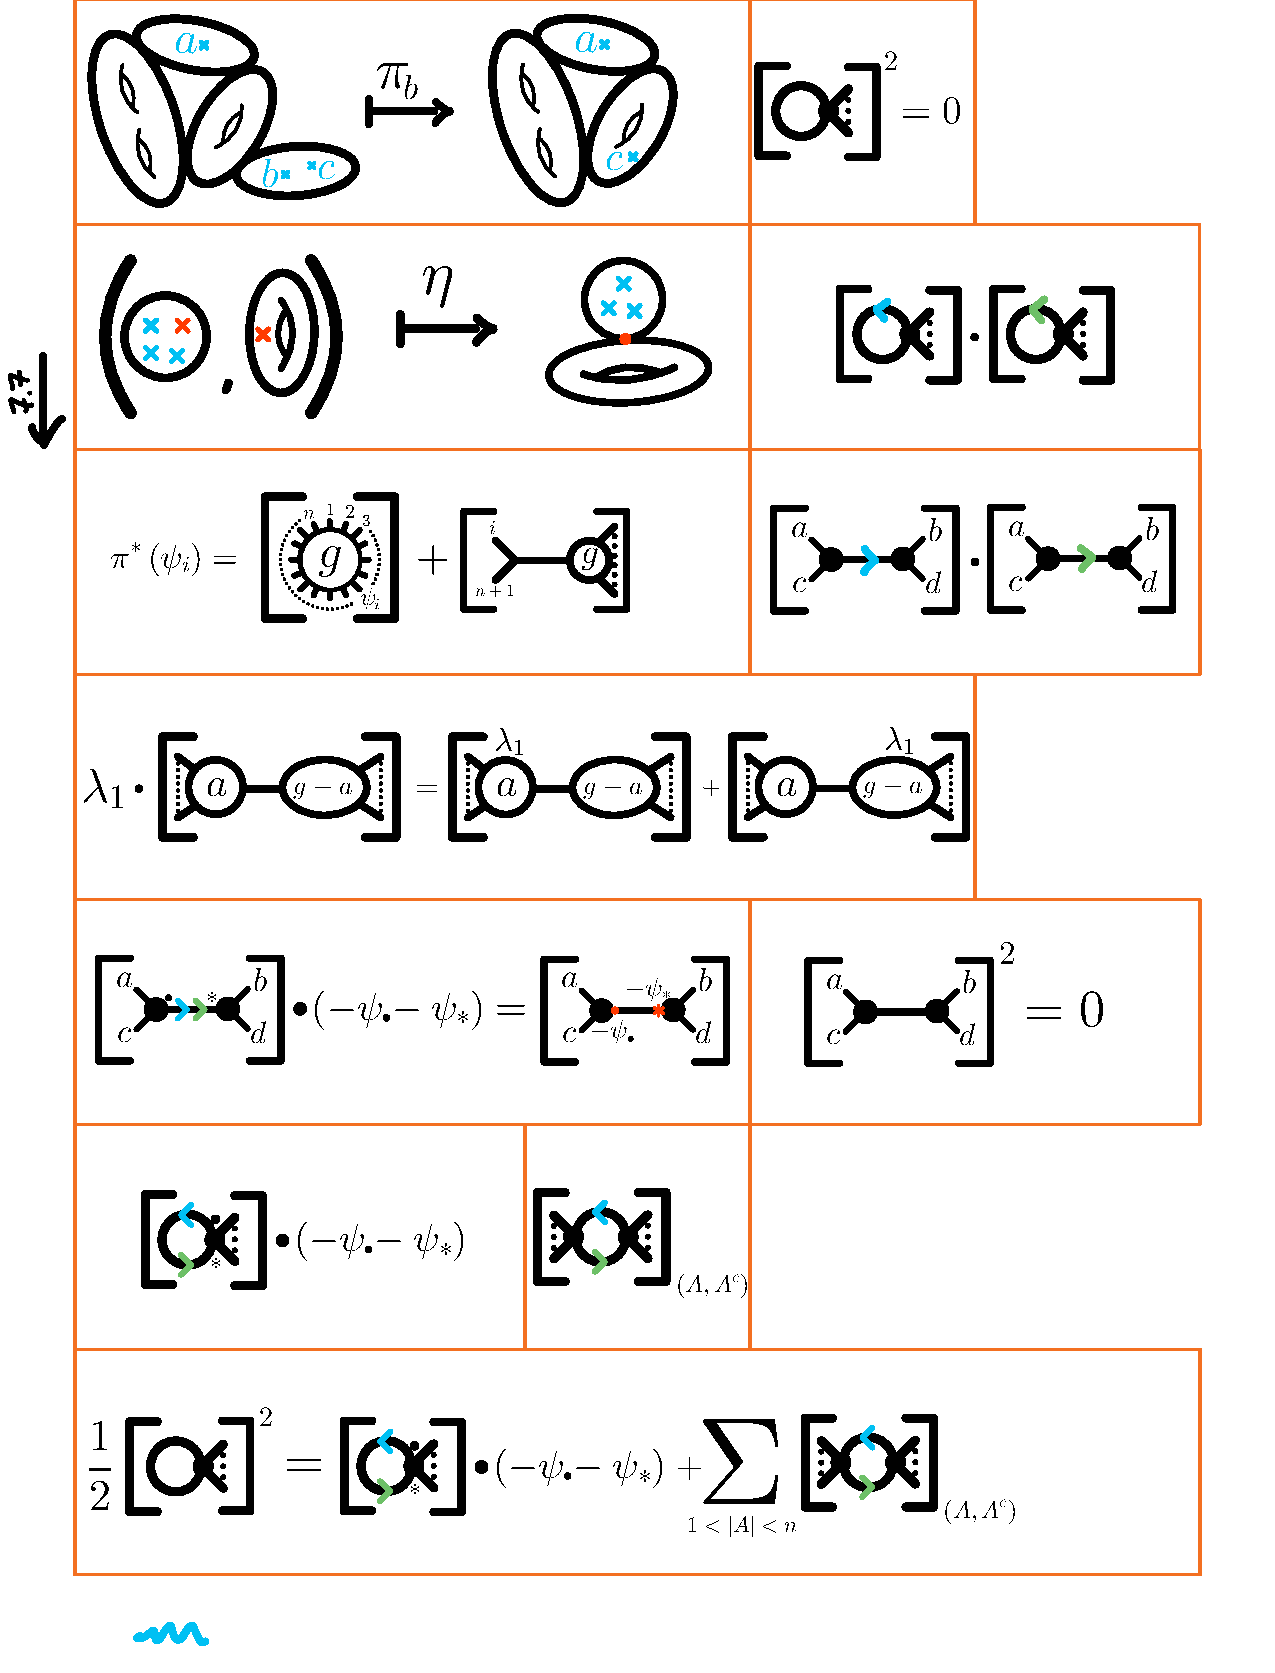
\includegraphics[width=0.5\textwidth, trim= 12.8cm 17.8cm 1.3cm 8cm,clip]{../figs/FigsDNnotability2.pdf}
        \caption{Factors identified with colors}
        \label{fig:divisor-squared-2-M04}
    \end{figure} 
    Once again let's follow the formula with care.
    \begin{enumerate}
        \item We look for all the graphs contracting into $\dl_{0,{ac}}$ once again. There's only $\dl_{0,{ac}}$ once more. This class has codimension 1, so we must multiply a psi-class to level the codimension.
        \item The edge in the result is bicolored to indicate that it is identified with the edges in the factors. Here we label the half-edges as $\8$ and $\ast$ so that we must multiply a psi-class $(-\psi_\8-\psi_\ast)$. This is the only difference with the previous calculation.
        \item The graph has no non-trivial automorphisms and no decorations.
    \end{enumerate}
    \begin{figure}[h!]
        \centering
        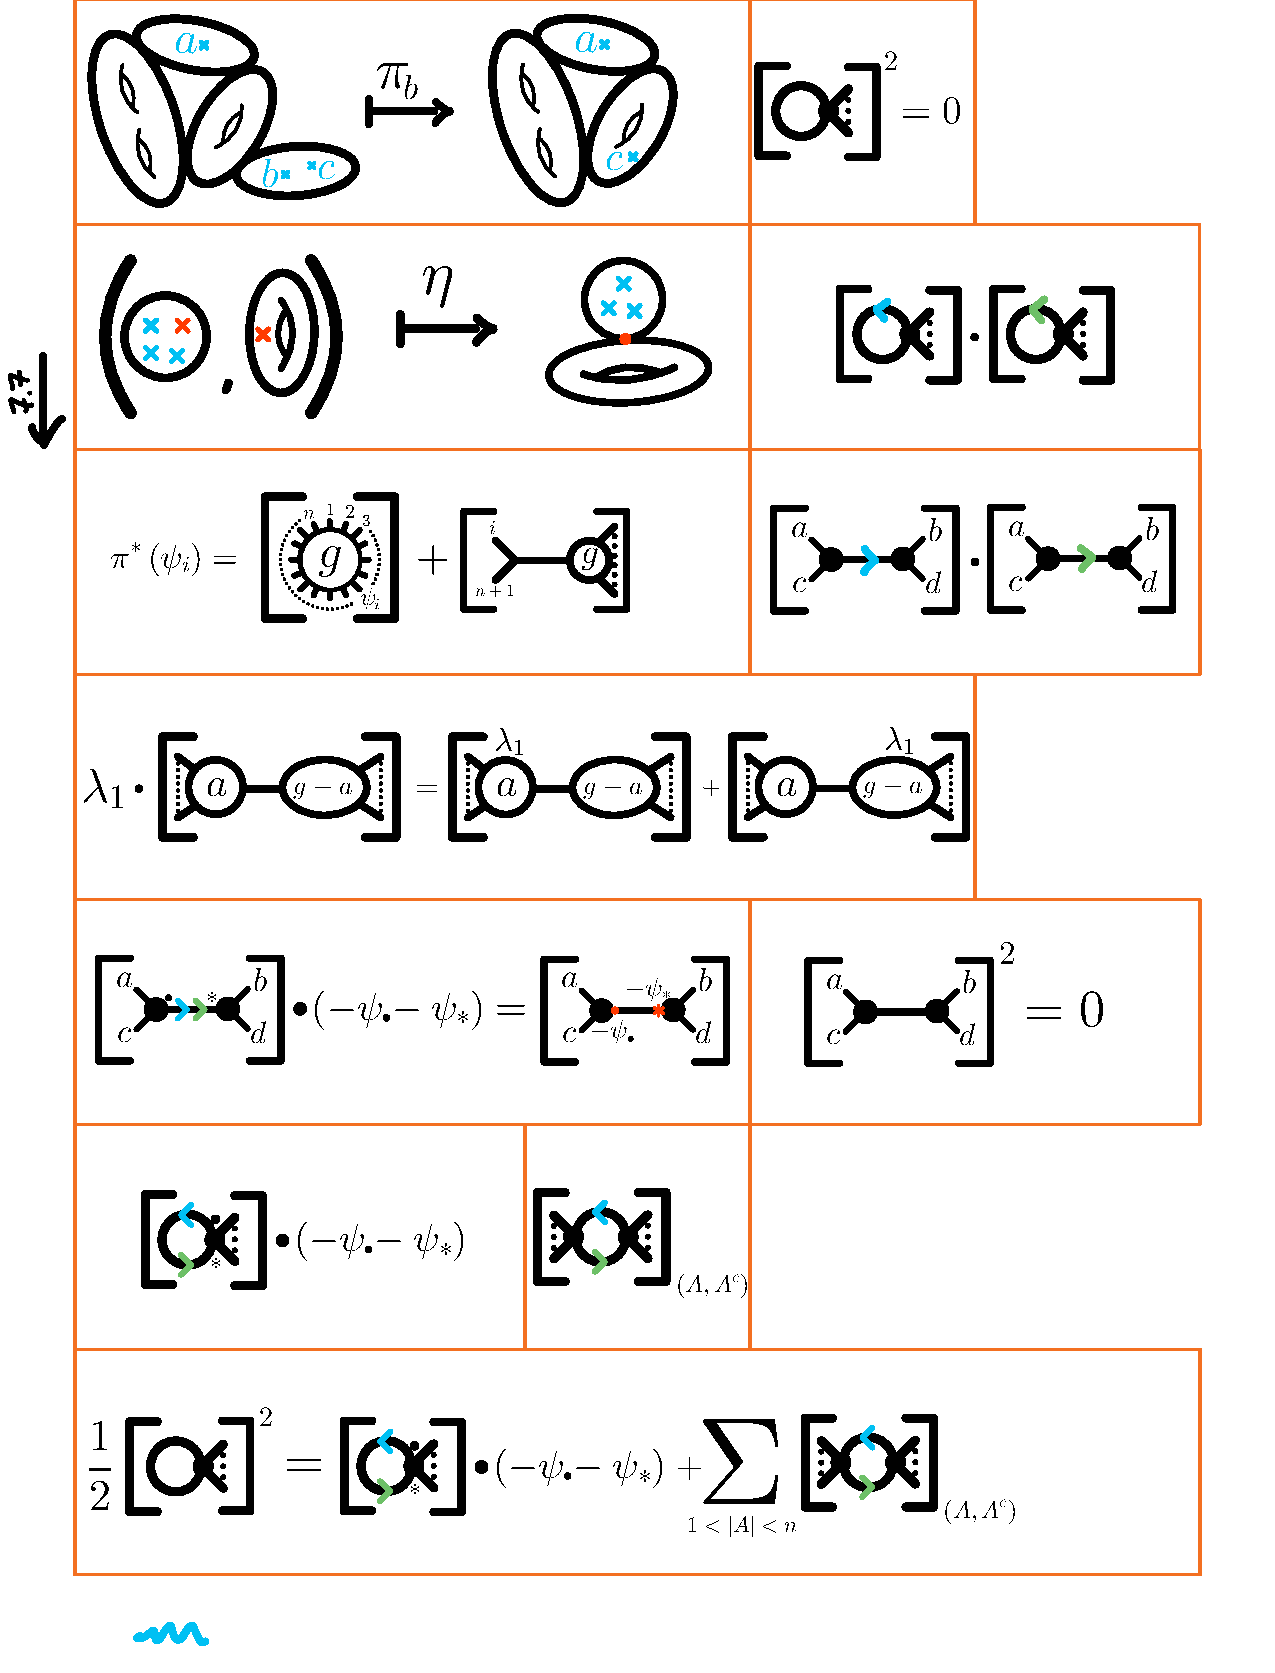
\includegraphics[width=0.7\textwidth, trim= 1.3cm 9.8cm 9cm 15.8cm,clip]{../figs/FigsDNnotability2.pdf}
        \caption{Multiplication result with psi-class}
        \label{fig:divisor-squared-3-M04}
    \end{figure} 
    The result is then 
    $$\dl_{0,{ac}}\.(-\psi_{\8}-\psi_{\ast})$$
    which we can see to be zero by a codimension count or as follows. 
    The stratum in question can be seen as the image of a gluing map:
    $$\eta\:\ov M_{0,\set{a,c,\8}}\x\ov M_{0,\set{b,d,\ast}}\to\ov M_{0,\set{a,\dots,d}},$$
    and when pulling back the psi-classes via the gluing map to the corresponding $M_{0,3}$'s we get the same psi-classes. These are $0$ in $M_{0,3}$ so that the result is also 0.
\end{Ex}

We climb up a couple of dimensions into $\ov M_{0,6}$ in the next example. This next classes will now have psi-classes multiplied and won't be zero!

\begin{Ex}
    Consider the intersection product in $\ov{M}_{0,6}$:
    $$\dl_{0,\set{a,b,c}}\dl_{0,\set{ab}}^2,$$
    \begin{figure}[h!]
        \centering
        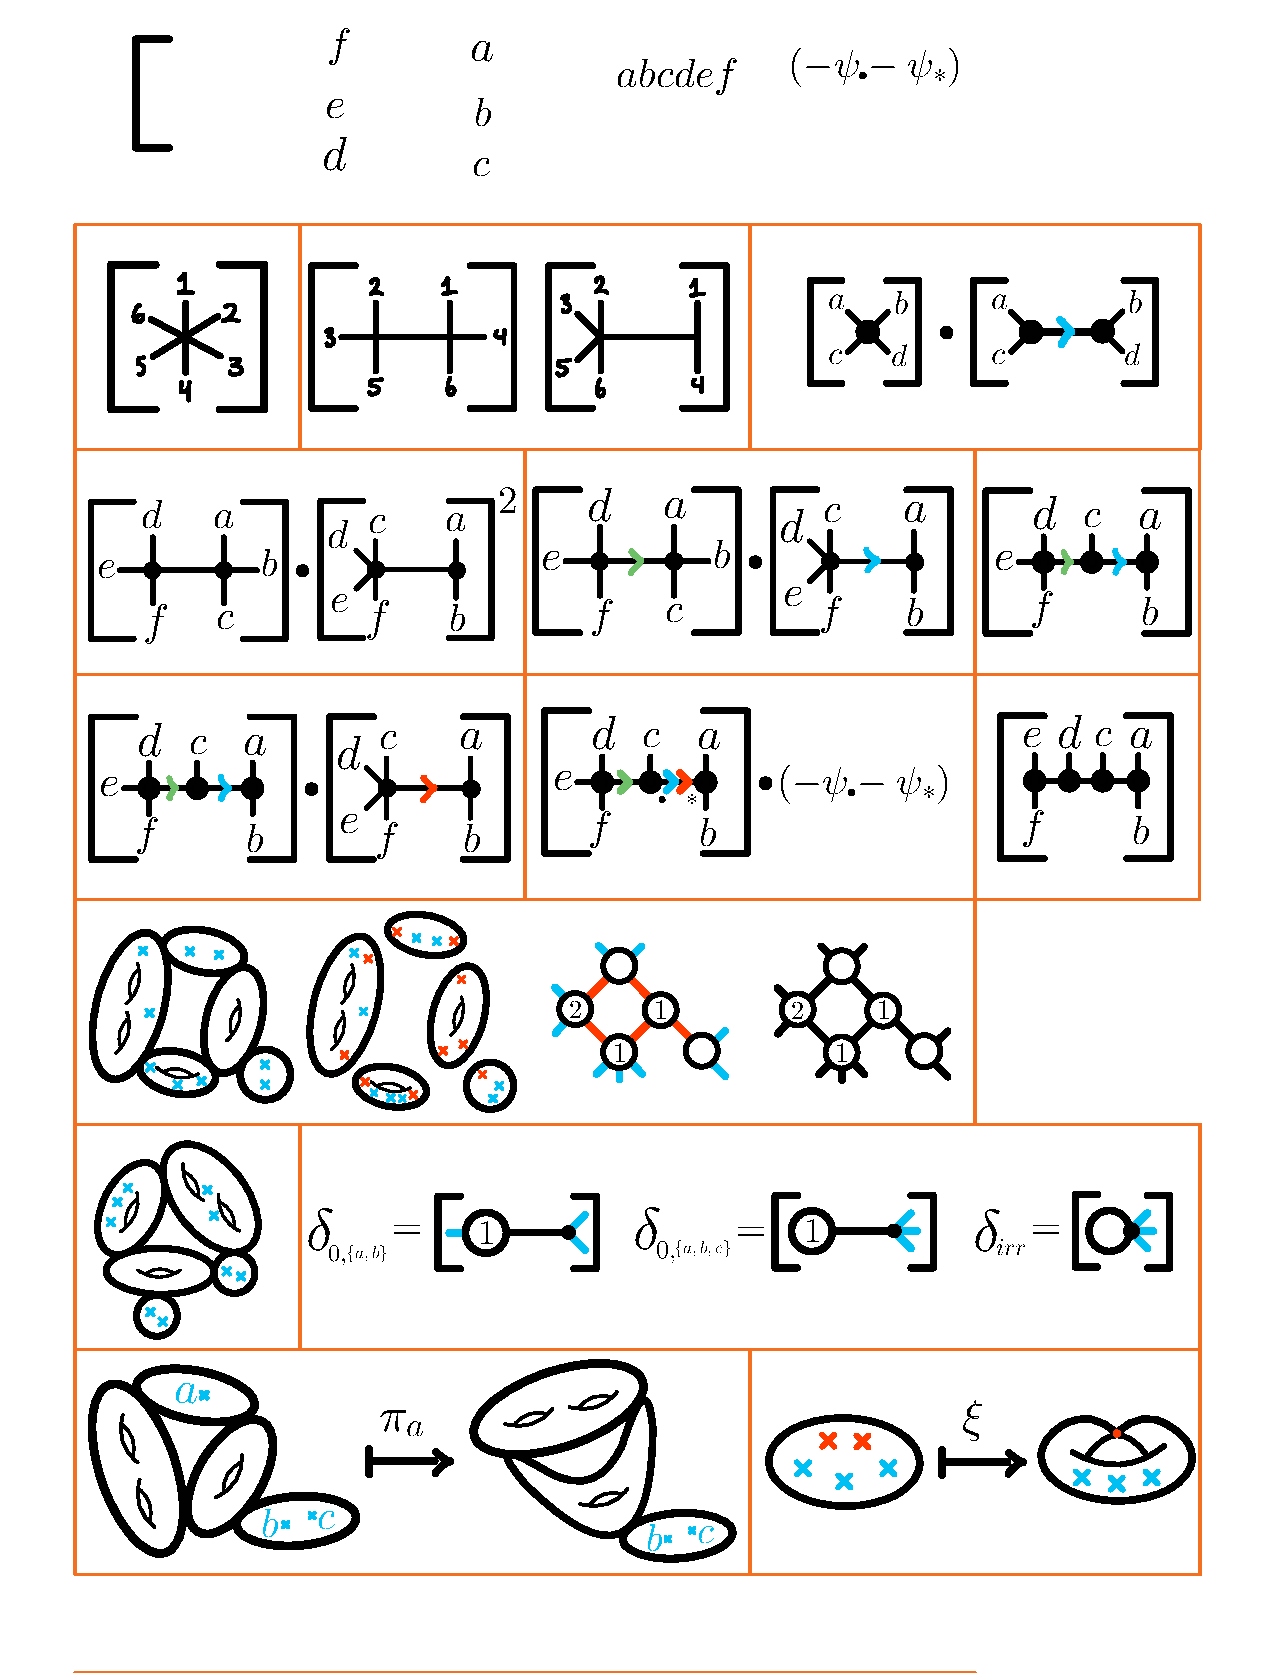
\includegraphics[width=0.5\textwidth, trim= 1.3cm 17.2cm 12.8cm 8cm,clip]{../figs/FigsDNnotability1.pdf}
        \caption{Multiplication of three divisors}
        \label{fig:three-divisors-1-M06}
    \end{figure}
    The expected codimension of the result is $3$ as every factor contributes $1$ codimension.\par
    We begin by multiplying a copy of $\dl_{0,\set{ab}}$ with $\dl_{0,\set{a,b,c}}$.
    \begin{figure}[h!]
        \centering
        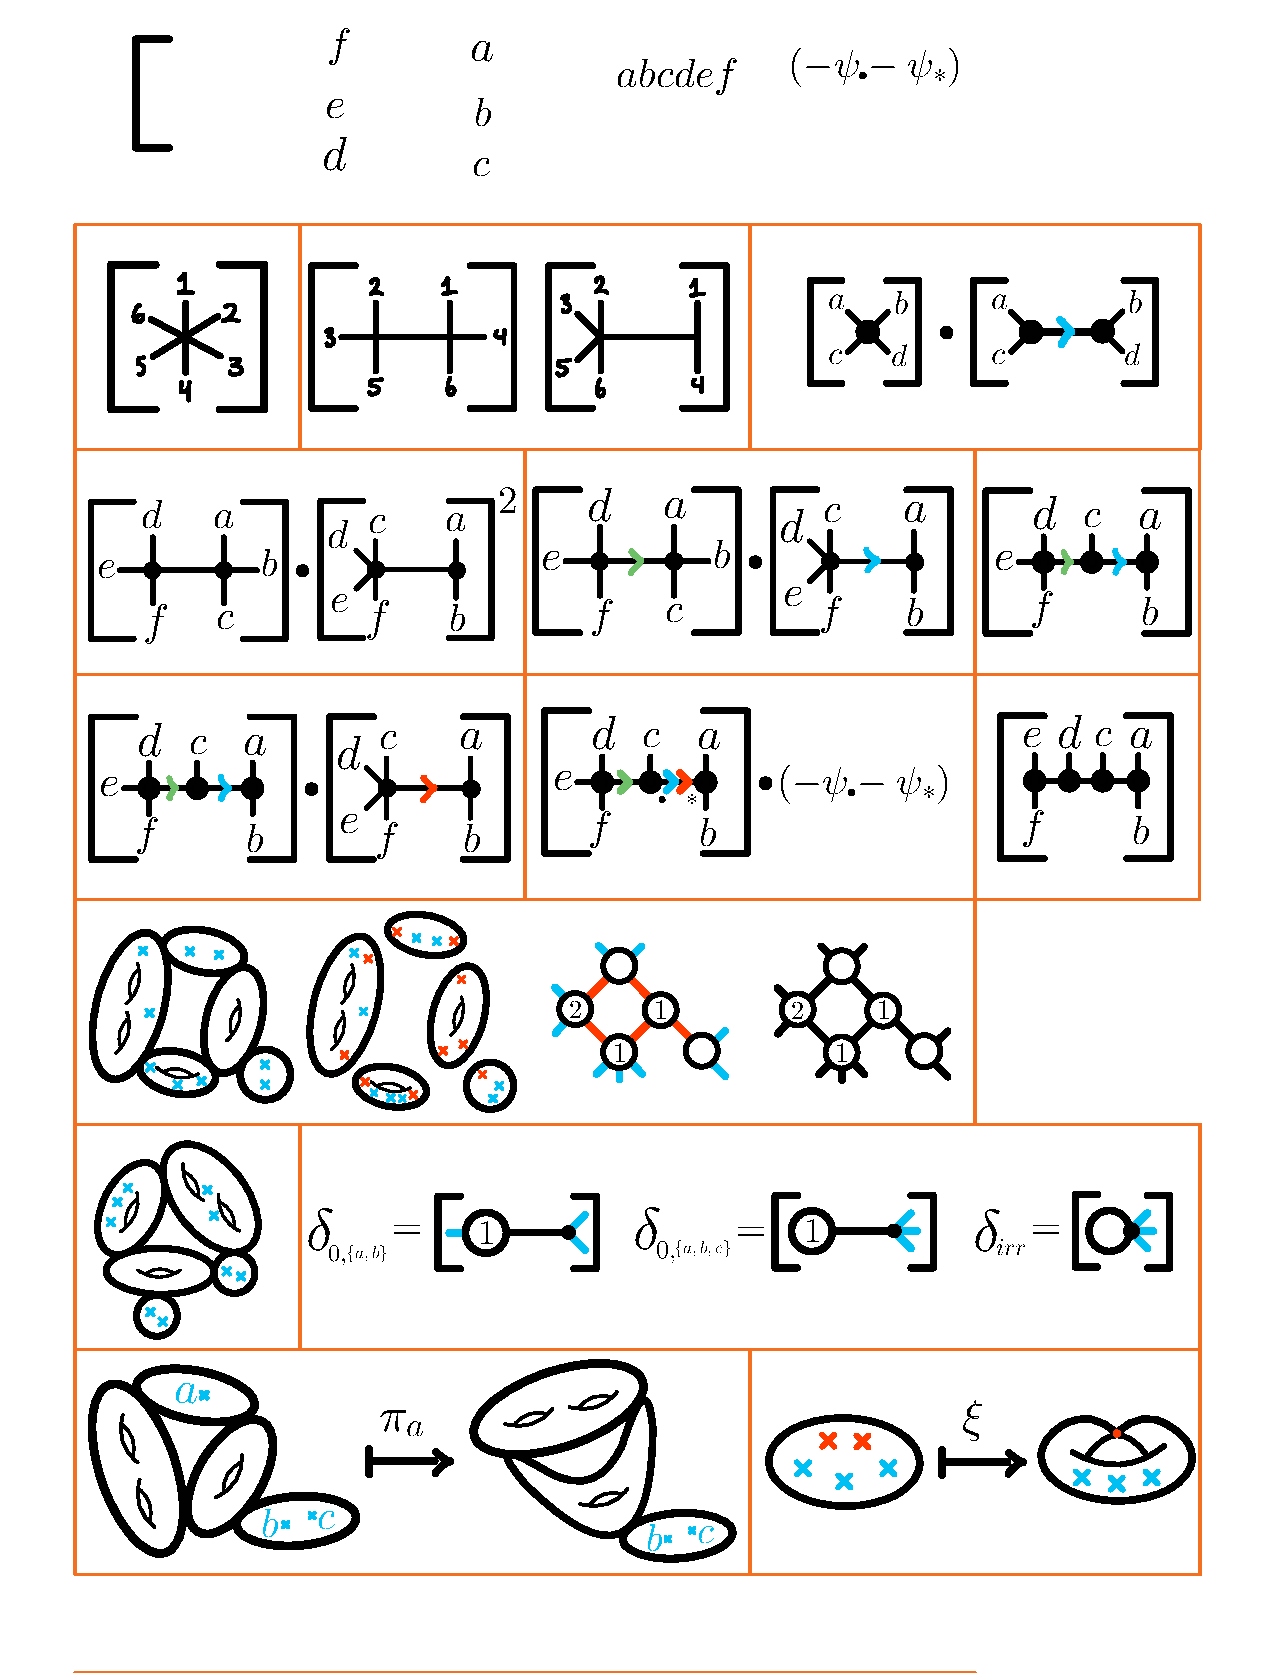
\includegraphics[width=0.5\textwidth, trim= 9cm 17.2cm 5.2cm 8cm,clip]{../figs/FigsDNnotability1.pdf}
        \caption{First multiplication}
        \label{fig:three-divisors-2-M06}
    \end{figure}
    We can only find one graph with contracts into these two. It's a codimension two class which has no non-trivial automorphisms nor decorations so we now multiply by the other divisor.
     \begin{figure}[h!]
        \centering
        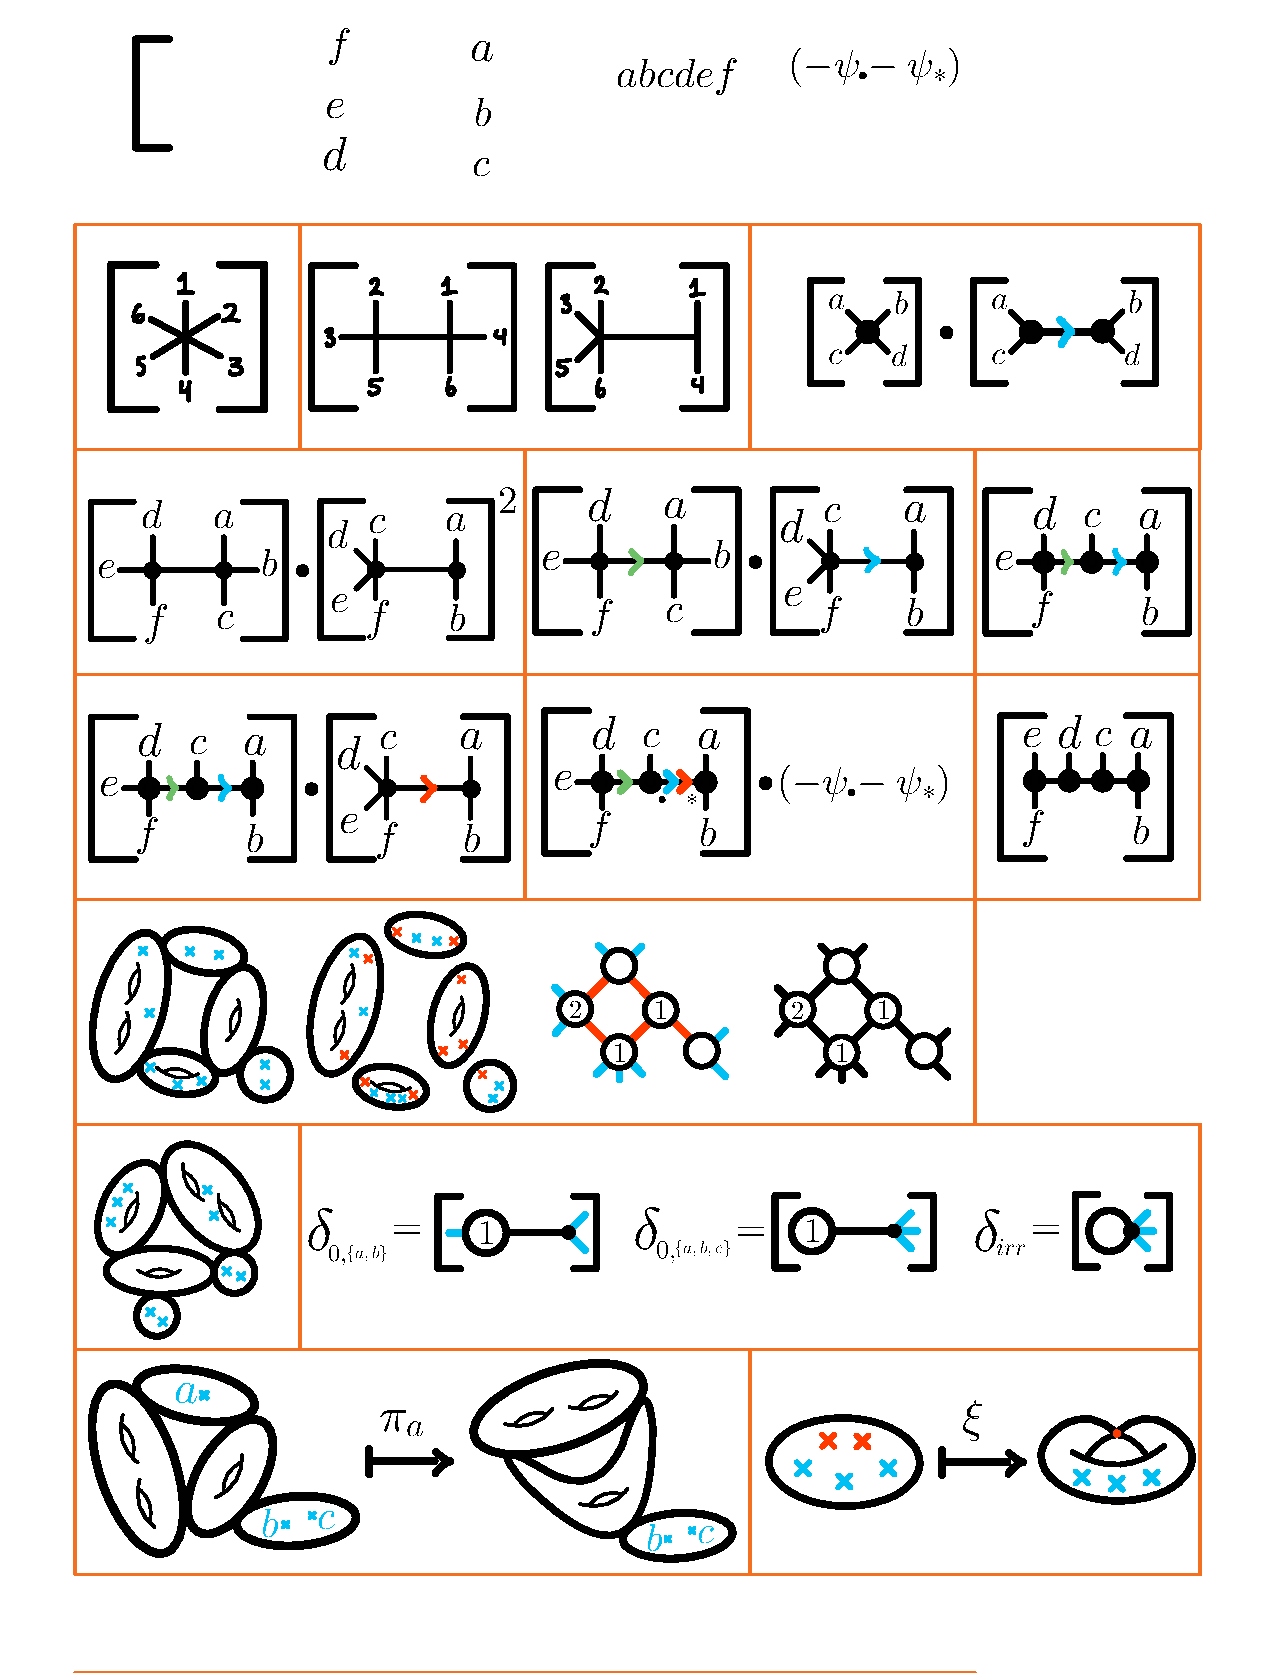
\includegraphics[width=0.5\textwidth, trim= 1.3cm 13.4cm 12.8cm 11.7cm,clip]{../figs/FigsDNnotability1.pdf}
        \caption{Second multiplication}
        \label{fig:three-divisors-3-M06}
    \end{figure}

    We expect the resulting graphs to have three edges as that would have codimension $3$. Creating such a graph is impossible, as any possible graph would non-generically contract into the factors.

      \begin{figure}[h!]
        \centering
        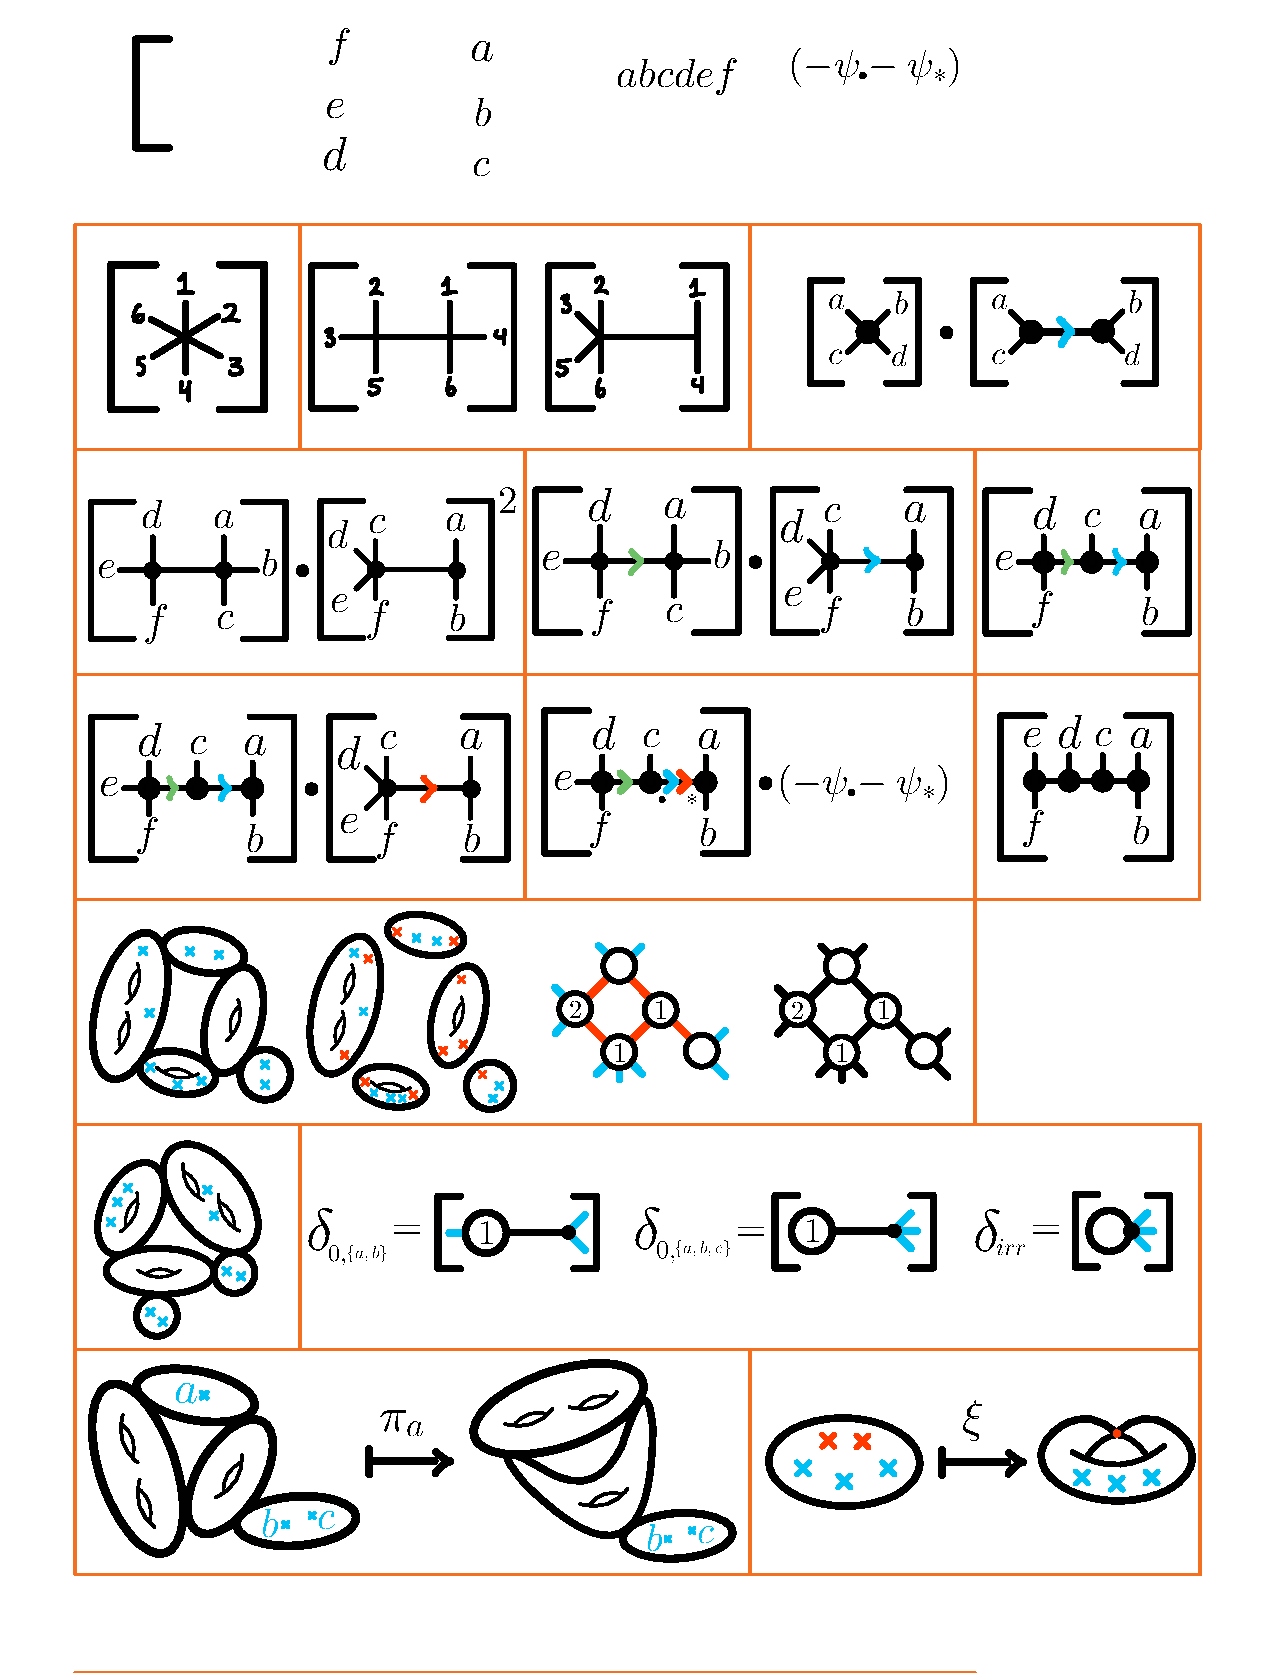
\includegraphics[width=0.25\textwidth, trim= 16.6cm 13.4cm 1.3cm 11.7cm,clip]{../figs/FigsDNnotability1.pdf}
        \caption{Non-generic contracting graph}
        \label{fig:three-divisors-4-M06}
    \end{figure}
    
    Such graph has three edges but \emph{they can't be colored} to respect the contraction. When contracting edges, the colors disappear so that we would have to leave an edge uncolored to respect the coloring.\par
    So the only possibility is the same graph that we just obtained but multiplied by a psi-class. One of the edges is bicolored and labeling the vertices of the corresponding edge as $\8$ and $\ast$ we get 
    $$\dl_{0,\set{ab}}\dl_{0,\set{a,b,c}}(-\psi_\8-\psi_\ast)$$
    This class has the correct codimension as the graph has two edges and the psi-class adds another codimension.
 \begin{figure}[h!]
        \centering
        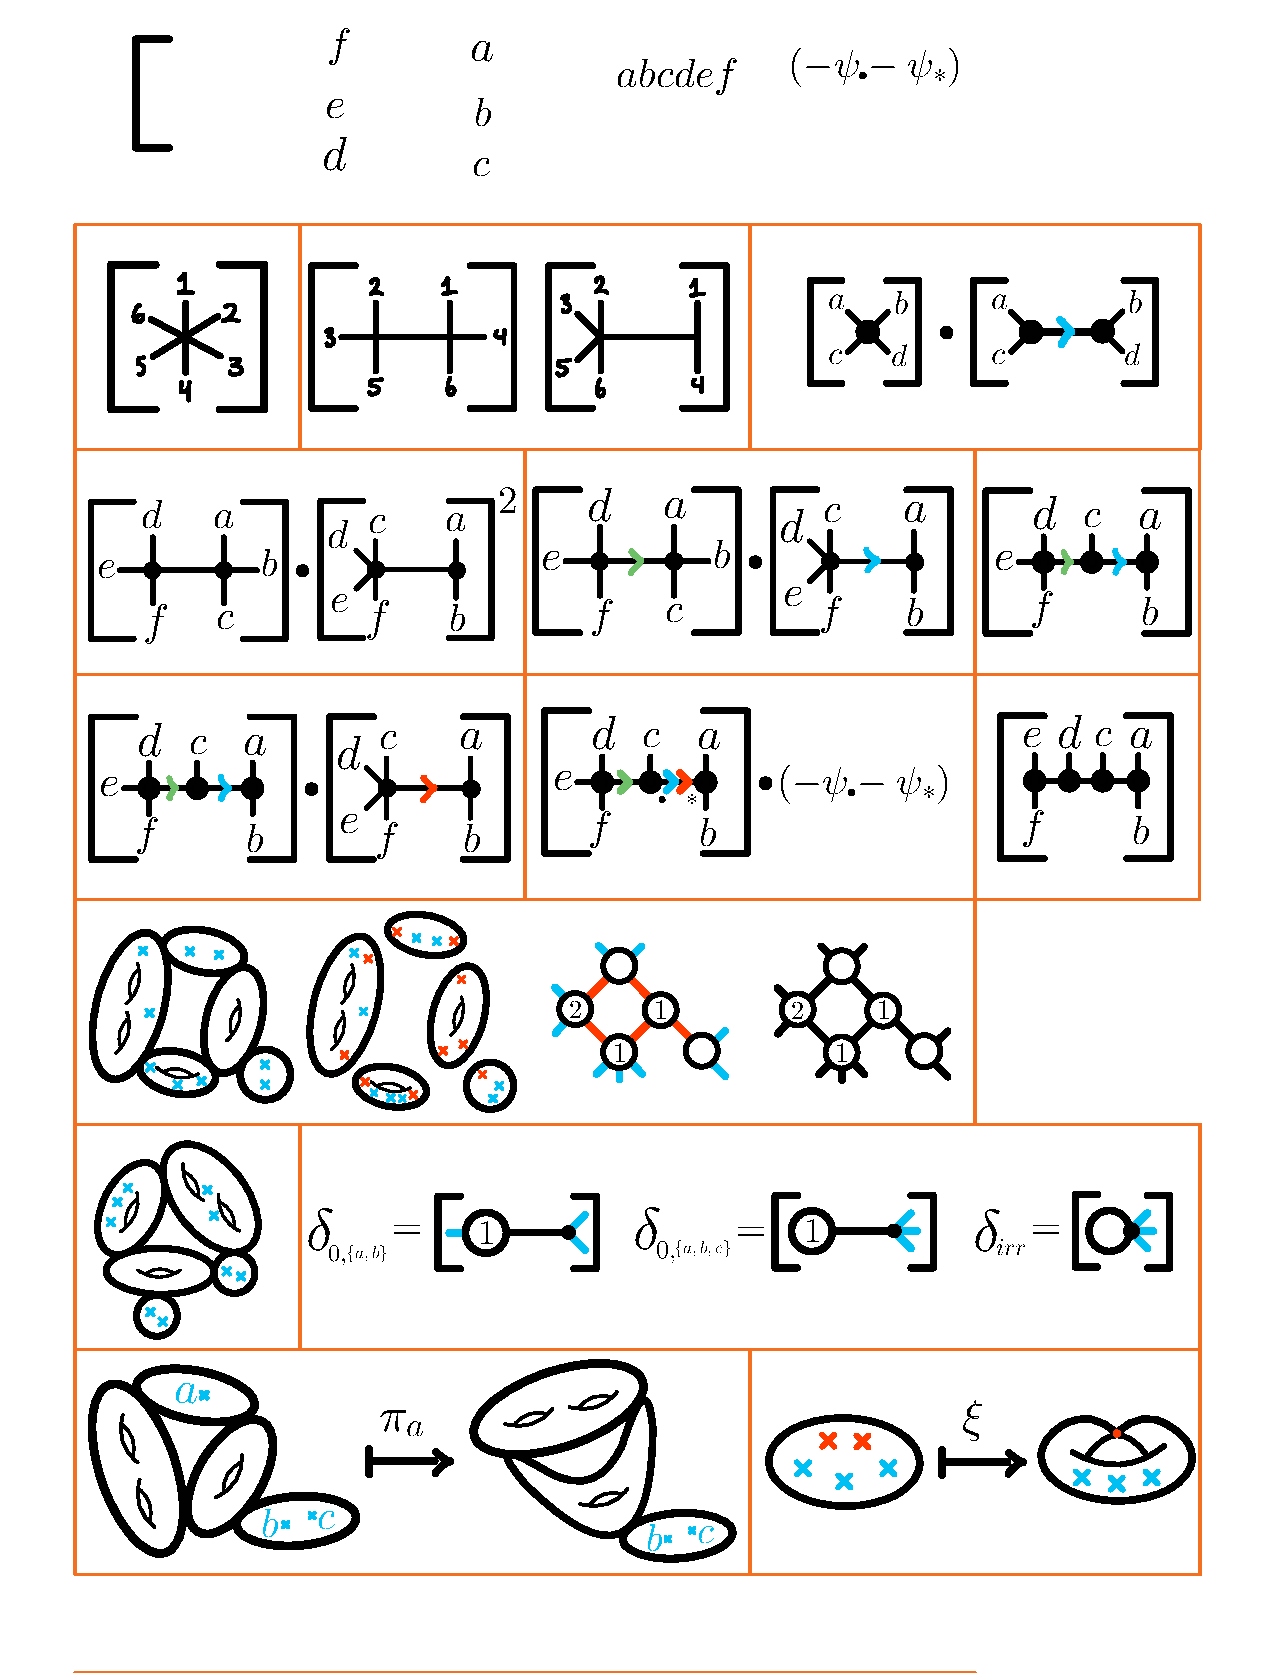
\includegraphics[width=0.5\textwidth, trim= 9cm 13.4cm 5.2cm 11.7cm,clip]{../figs/FigsDNnotability1.pdf}
        \caption{Final result of product}
        \label{fig:three-divisors-5-M06}
    \end{figure}

\end{Ex}

\begin{Ex}[\cite{ZvonkineIntro}, Exercise 2.4]\label{ex-unexpectedly-zero-square}
\begin{figure}[h!]
        \centering
        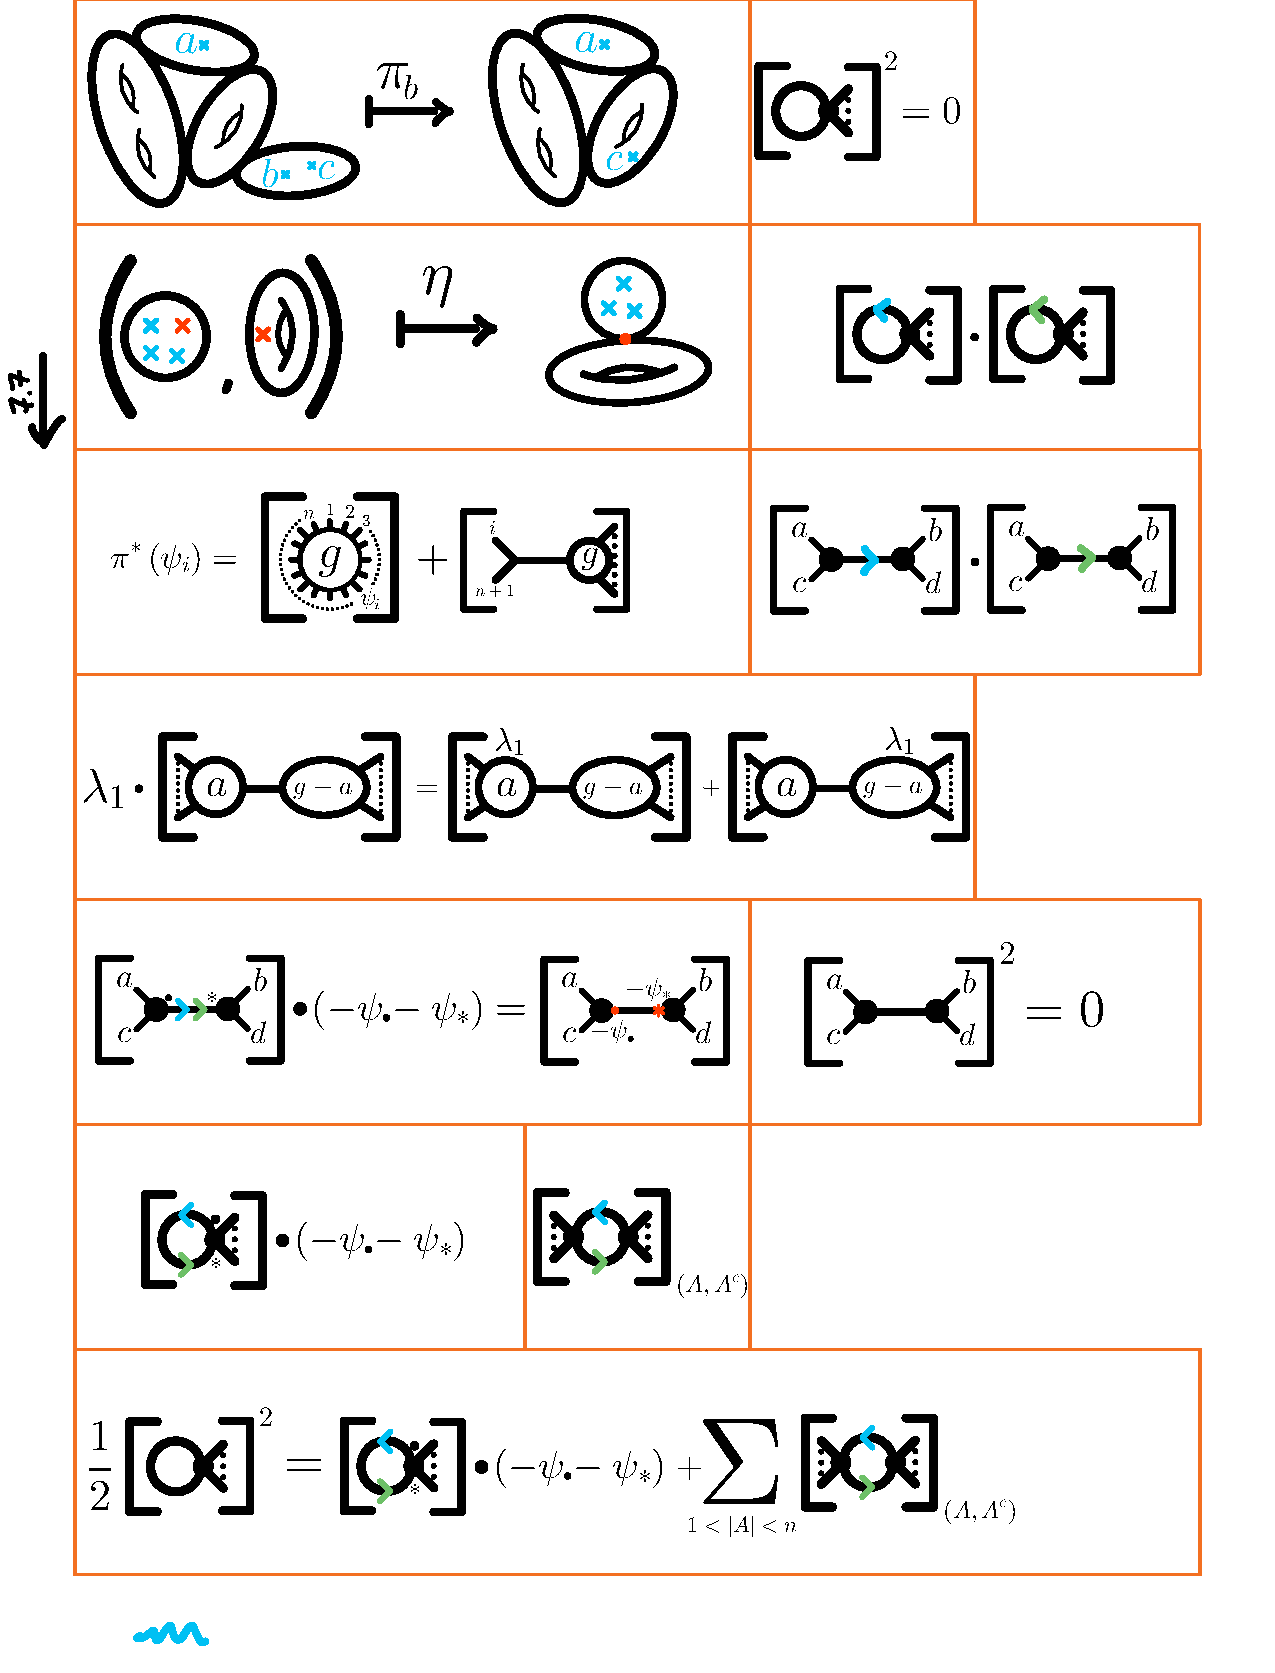
\includegraphics[width=0.35\textwidth, trim= 12.8cm 25.5cm 5.2cm 0.5cm,clip]{../figs/FigsDNnotability2.pdf}
        \caption{Irreducible divisor squared}
        \label{fig:irr-squared-1}
    \end{figure}

   Recall the irreducible divisor of stable curves with one non-separating node $\dl_{\text{irr}}\in\ov{M}_{1,n}$. We will show that $\dl_{\text{irr}}^2=0$. Following the idea from figure \ref{fig:divisor-squared-2-M04} in the divisor squared example for $\ov{M}_{0,4}$, we separate the product into two factors and color.

   \begin{figure}[h!]
        \centering
        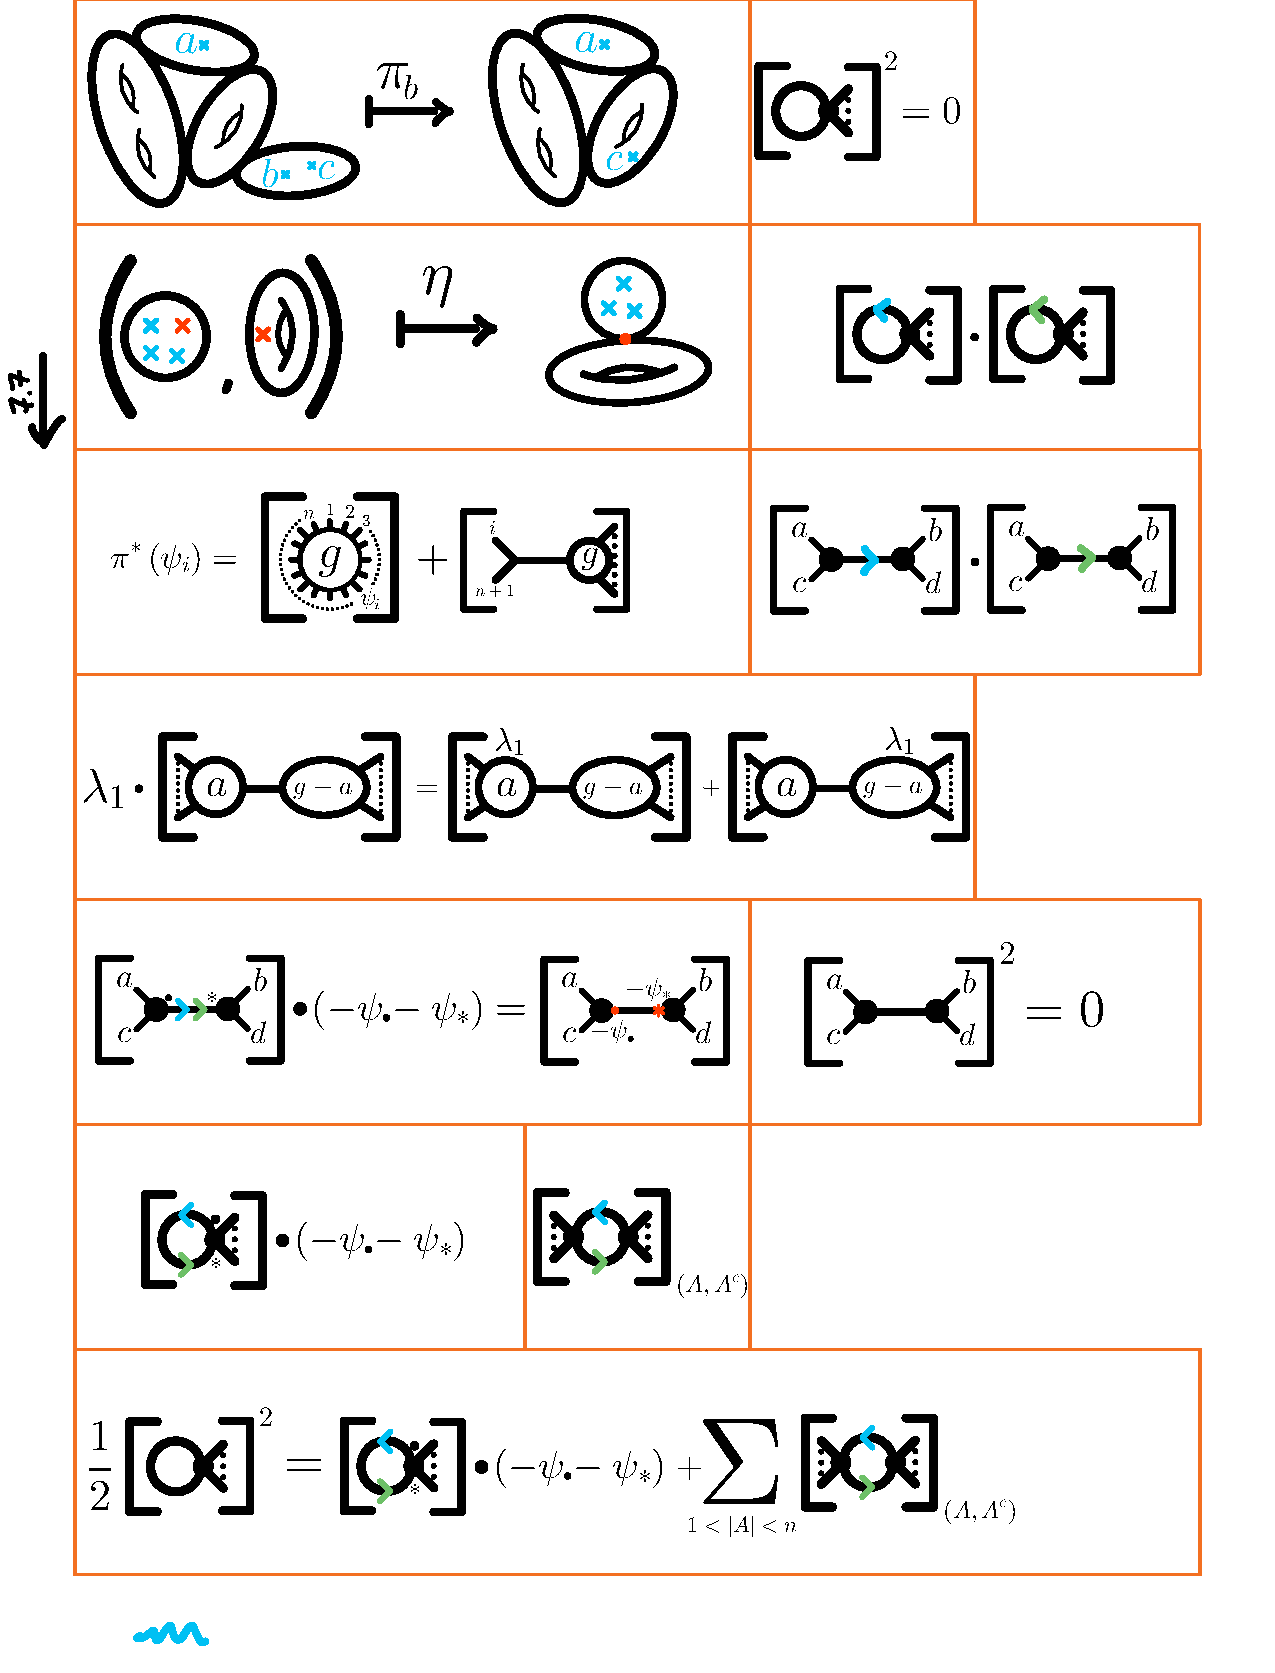
\includegraphics[width=0.4\textwidth, trim= 14.1cm 21.3cm 2.7cm 4.3cm,clip]{../figs/FigsDNnotability2.pdf}
        \caption{Separated product with edges colored}
        \label{fig:irr-squared-2}
    \end{figure}

    There's two kinds of graphs which contract into this one. First itself, with the edge bicolored. Due to this we have to add a psi-class because the edge is identified with both factors.

     \begin{figure}[h!]
        \centering
        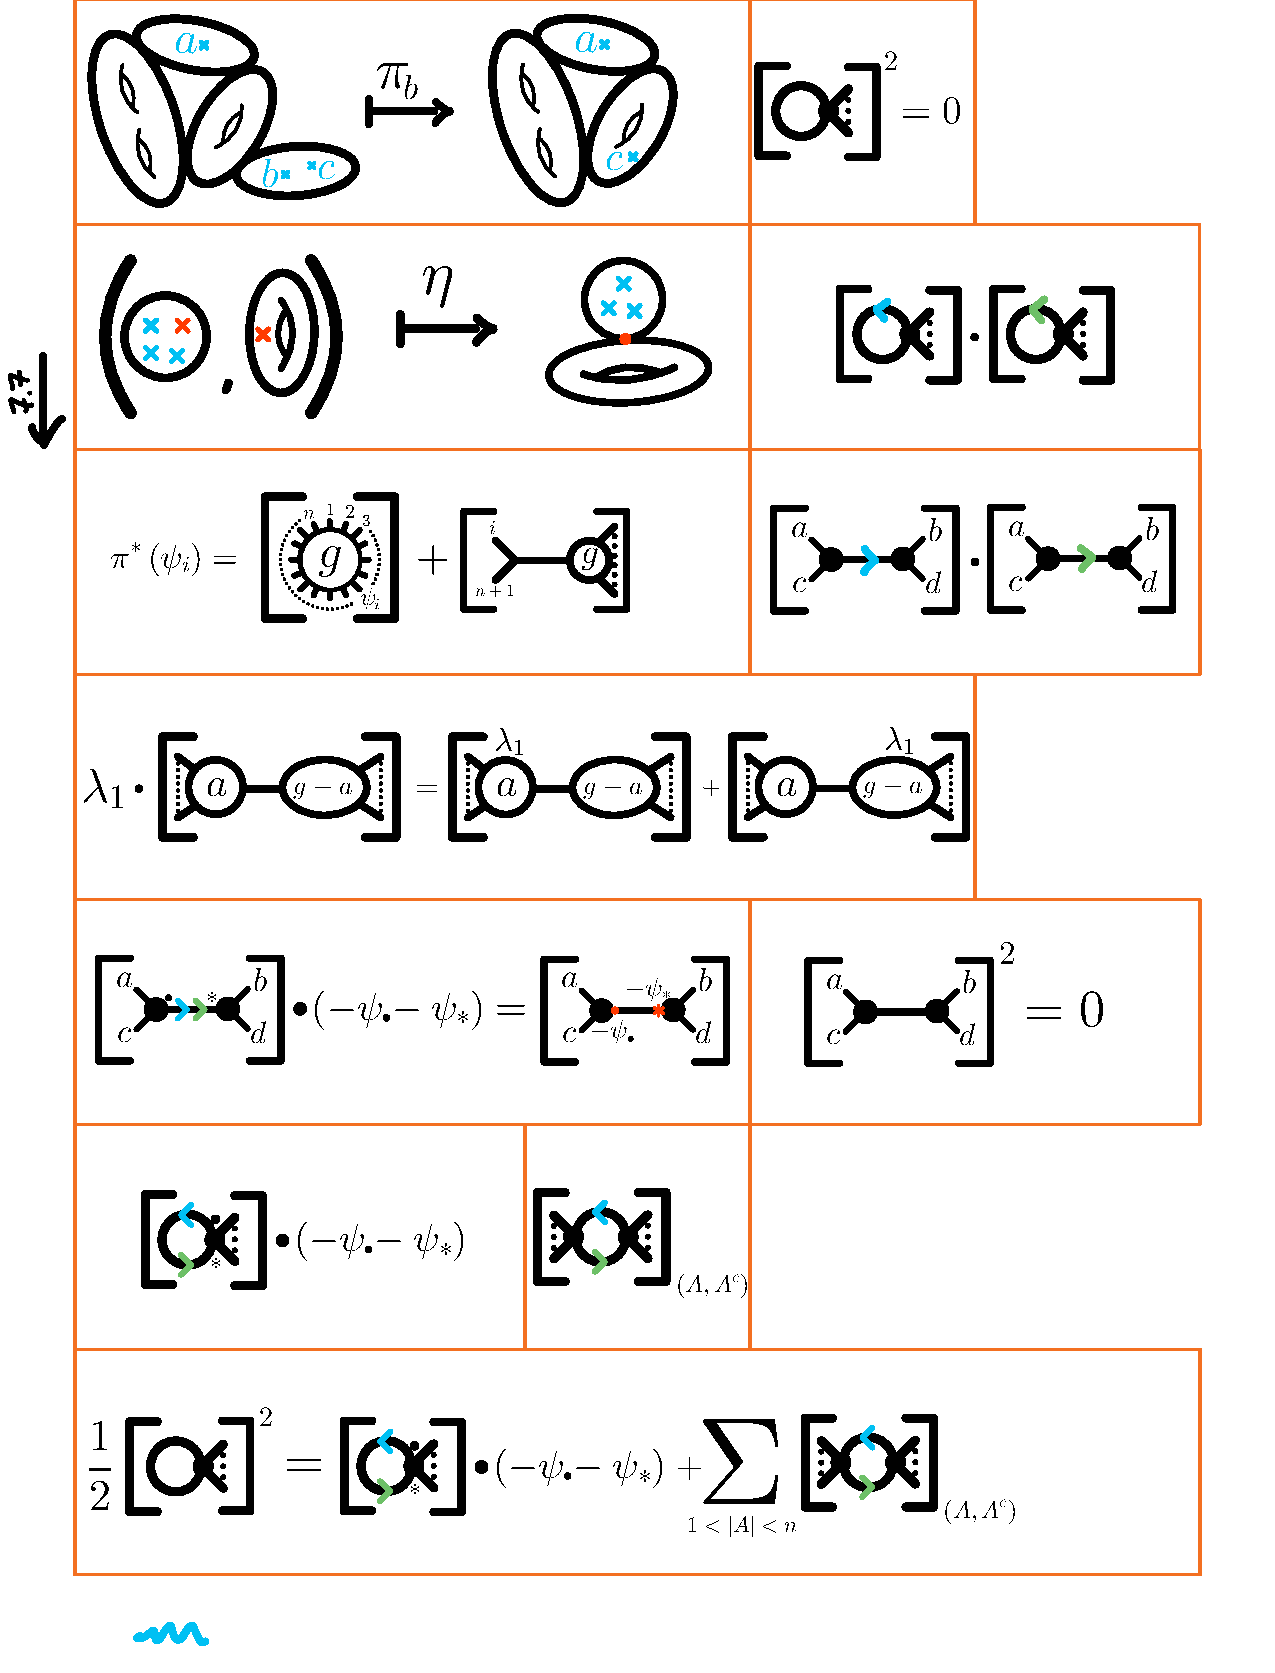
\includegraphics[width=0.5\textwidth, trim= 2cm 6.5cm 13.5cm 20cm,clip]{../figs/FigsDNnotability2.pdf}
        \caption{Irreducible divisor with psi-class to correct codimension}
        \label{fig:irr-squared-3}
    \end{figure}
    Besides this one, we have $2^n-2$ other possible graphs representing curves with two components with the marks distributed among them. These are indexed by $A\subseteq\set{n}$ containing at least one element. On one component the curve has $|A|$ marks, and on the other side, $n-|A|$. The components are joined by two nodes so it has the correct codimension.
     \begin{figure}[h!]
        \centering
        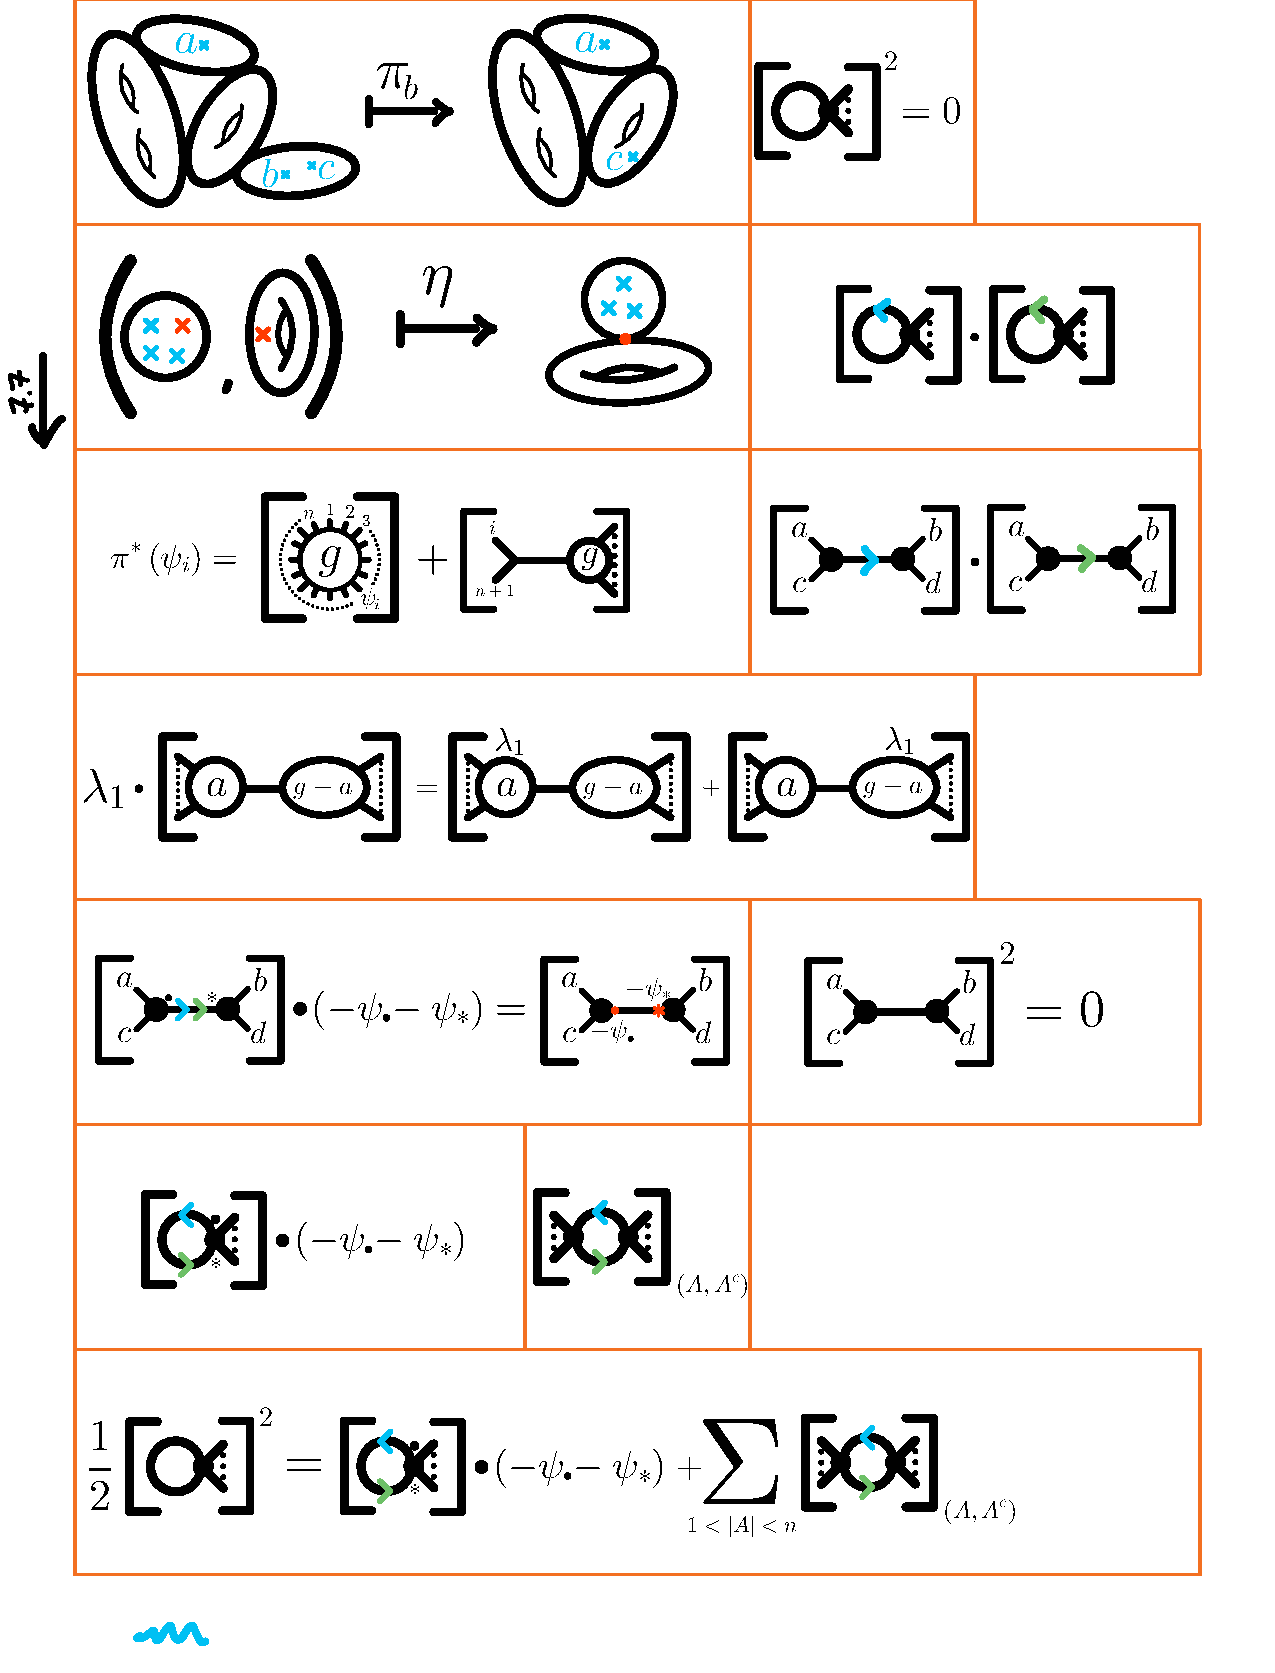
\includegraphics[width=0.3\textwidth, trim= 9cm 6.2cm 8.92cm 20cm,clip]{../figs/FigsDNnotability2.pdf}
        \caption{Codimension 2 strata indexed by $A$}
        \label{fig:irr-squared-4}
    \end{figure}
    So in total, the sum of these classes gives us the result of squaring $\dl_{\text{irr}}$. We get a factor of 2 in each of the terms accounting for the automorphisms which we turn to the other side of the equation as a half factor.%check automorphisms at some point.

     \begin{figure}[h!]
        \centering
        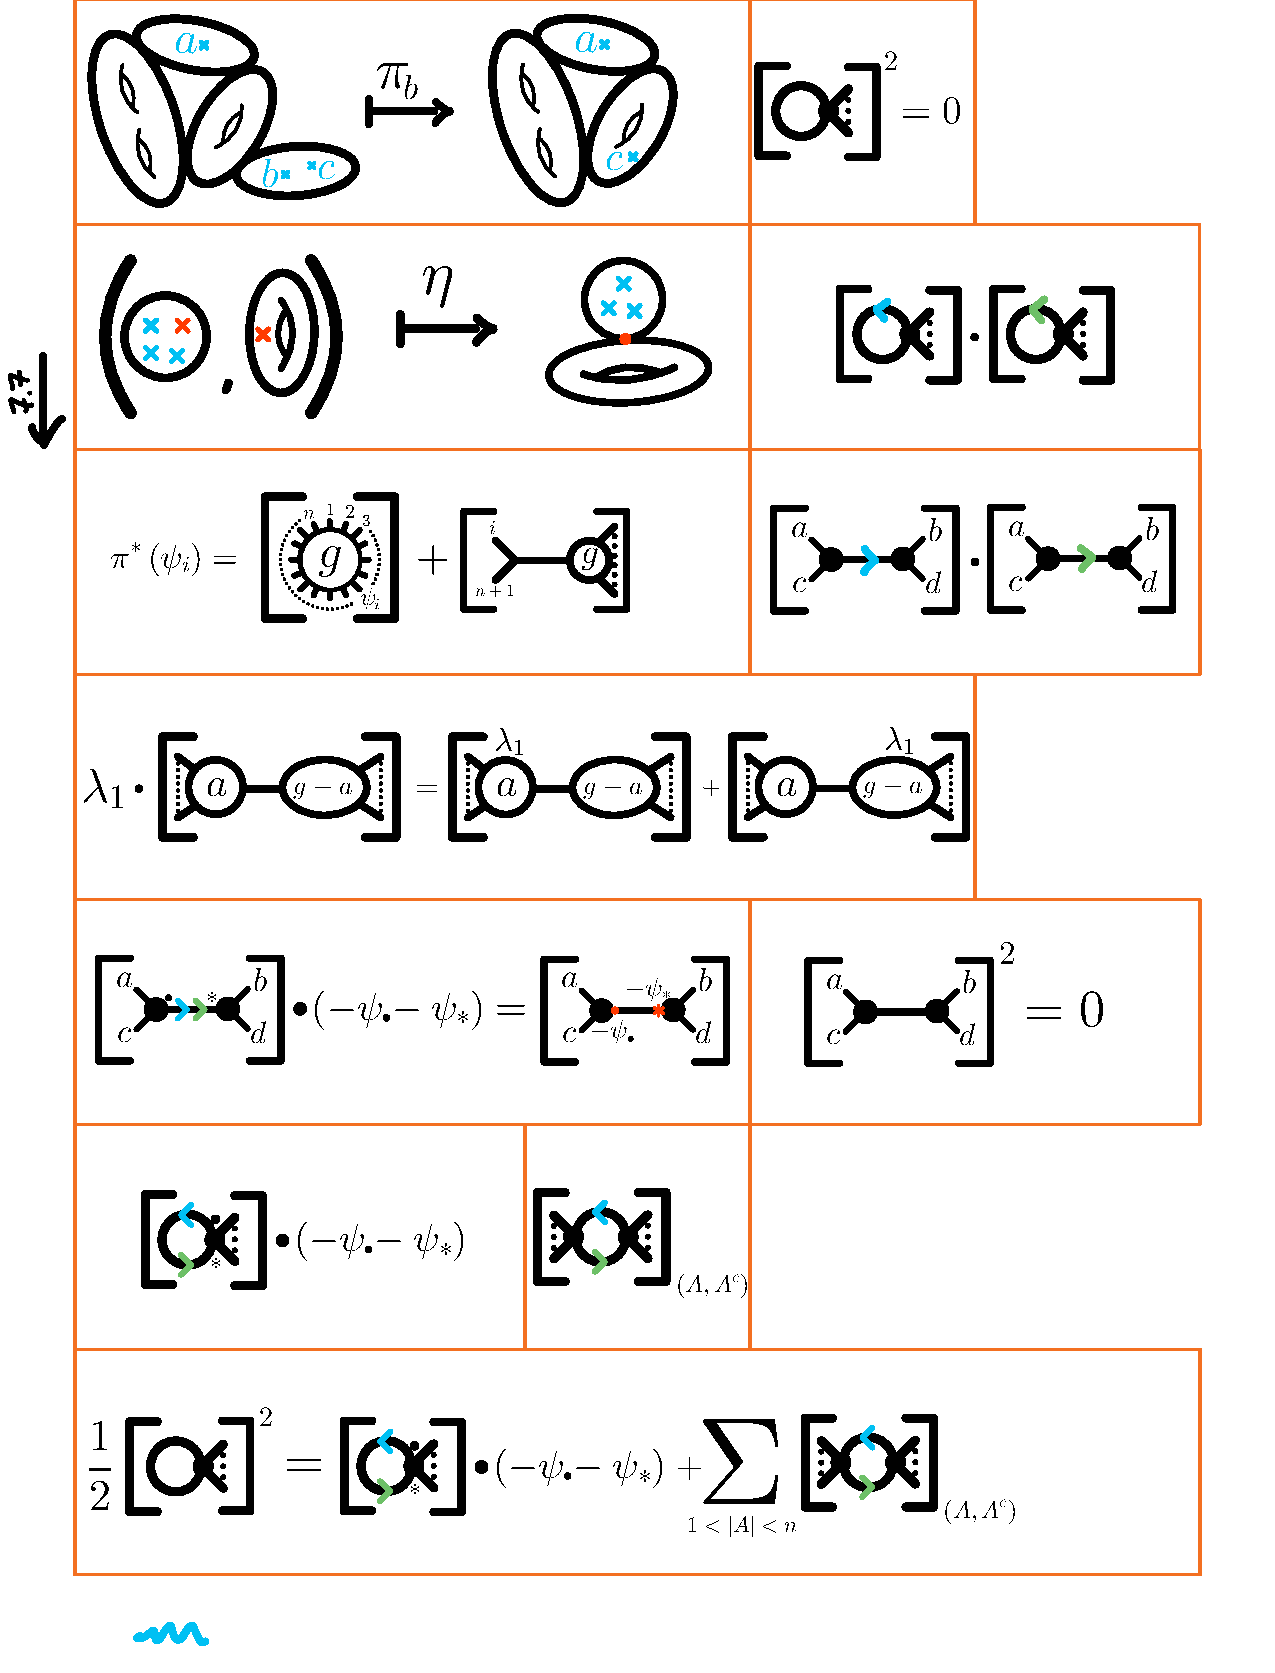
\includegraphics[width=0.95\textwidth, trim= 1.3cm 2.3cm 4.3cm 23.8cm,clip]{../figs/FigsDNnotability2.pdf}
        \caption{Final sum with all strata}
        \label{fig:irr-squared-5}
    \end{figure}
    Finally observe the restriction of the psi-classes $\psi_\8,\psi_\ast$ to the divisor $\dl_{\text{irr}}$ can be realized as the sum of the codimension 2 graphs as in the right.\par
    This comes in part because of lemma \ref{lem:divisor-sum-identity-psi-class} which allows us to express the sum of psi-classes:
    $$\psi_\8+\psi_\ast=\sum_{\substack{\8\in A,\ \ast\not\in A\\|A|\geq 1}}\dl_{0,A},\word{in}\ov{M}_{0,\bonj{n}\cup\set{\8,\ast}}.$$
    Then restricting to the divisor $\dl_{\text{irr}}$ is to glue $\8$ and $\ast$ together. Switching the sign and canceling gives us the desired result. 
\end{Ex}

\section{Integration}

Fulton and Pandharipande \cite{FPNotes} give us the definition of the integral that we will use. 

\begin{Def}[\cite{FPNotes} pg. 2]
    For a complete variety, $c\in A^\ast(X)$ and $\bt\in A_k(X)$ then 
    $$\int_\bt c=\deg(c_k,\bt)$$
    where $c_k$ is the component of $c$ in $A^k(X)$ and $(c_k,\bt)$ is the evaluation of $c_k$ on $\bt$ giving us a zero cycle. When $V$ is a closed, pure-dimensional subvariety of $X$, then we write 
    $$\int_V c\word{instead of}\int_{\bonj{V}}c.$$
\end{Def}

In our case, this can be seen as the pushforward of the constant map from $\ov M_{g,n}$ to a point. 
$$A^\ast(\ov{M}_{g,n})\xrightarrow[]{c_\ast}A^\ast(\pt)\quad\To\quad \int_{\ov{M}_{g,n}}\defeq c_\ast.$$

\subsection{The string equation}

\begin{Ex}
Consider the integral 
$$I=\int_{\ov{M}_{0,4}}\psi_1$$
we apply the forgetful map identity for the psi-class (as seen in example \ref{ex-psi-class-forgetful-identity}) to get
$$I=\int_{\ov{M}_{0,4}}\pi_2^\ast(\psi_1)+\Im s_1=\int_{\ov{M}_{0,4}}0+\dl_{0,\set{1,4}}.$$
Coupling this divisor against the fundamental class gives us a zero-cycle, and as there's no coefficients we get a $1$. Therefore 
$$I=\int_{\ov{M}_{0,4}}\psi_1=1$$
\end{Ex}

We can now continue into integrals involving higher powers of psi-classes. For this, let's take into account the following diagram

$$
\begin{tikzcd}
 \ov{M}_{g,n+1}\arrow[dr,"c"]\arrow[dd,"\pi"']&\\
 &\pt\\
 \ov{M}_{g,n}\arrow[ur,"\widetilde{c}"']&
\end{tikzcd}
\To
\begin{tikzcd}
 A^\ast(\ov{M}_{g,n+1})\arrow[dr,"c_\ast=\displaystyle\int_{\ov{M}_{g,n+1}}"]\arrow[dd,"\pi_\ast"']&\\
 &A^\ast(\pt)\\
 A^\ast(\ov{M}_{g,n})\arrow[ur,"\widetilde{c}_\ast=\displaystyle\int_{\ov{M}_{g,n}}"']&
\end{tikzcd}
$$

Observe that via the forgetful map, we may integrate classes from the upper moduli space by pushing them forward and then integrating on the moduli space on the bottom. This means that
$$\int_{\ov{M}_{g,n+1}}\al=\int_{\ov{M}_{g,n}}\pi_\ast\al,\word{for}\al\in A^\ast(\ov M_{g,n+1}).$$
To work with pushforwards and psi-classes involving pullbacks, we must use the projection formula for the Chow ring. 

\begin{Prop}
    %https://mathoverflow.net/questions/67228/where-do-all-these-projection-formulas-come-from
    Given a proper map $f\: X\to Y$ between nonsingular algebraic varieties and cycle classes $\al\in A^\ast(X),\bt\in A^\ast(Y)$ we have
    $$f_\ast(\al\.f^\ast(\bt))=f_\ast(\al)\.\bt.$$
\end{Prop}

The following lemma for reduction in power of the psi-class also comes in handy.

\begin{Lem}
For a forgetful map $\pi_j$ and a psi-class $\psi_i$, we have 
$$\psi_i^k=(\pi_j^\ast\psi_i)^{k-1}(\pi_j^\ast\psi_i+\dl_{0,\set{ij}}),\quad k\in\bZ_{\geq 0}.$$
\end{Lem}

\begin{ptcbp}
    We may first apply the projection formula \ref{ex-psi-class-forgetful-identity} for the psi-class
    $$\psi_i^k=\psi_i(\pi_j^\ast\psi_i+\dl_{0,\set{ij}})^{k-1}.$$
    Now we expand the binomial and distribute the outside psi-class as follows 
    \begin{align*}
        =&\psi_i\sum_{\l=0}^{k-1}\binom{k-1}{\l}(\pi_j^\ast\psi_i)^\l(\dl_{0,\set{ij}})^{k-1-\l}\\
        =&\left(\psi_i\dl_{0,\set{ij}}^{k-1}+(k-1){\psi_i}\dl_{0,\set{ij}}^{k-2}\pi_j^\ast\psi_i+\dots\right.\\
        &\left.\phantom{\left(\right.}+(k-1)\psi_i\dl_{0,\set{ij}}(\pi_j^\ast\psi_i)^{\l-1}+\psi_i(\pi_j^\ast\psi_i)^{k-1}\right)\\
        =&\psi_i(\pi_j^\ast\psi_i)^{k-1}\\
        =&(\pi_j^\ast\psi_i)^{k-1}(\pi_j^\ast\psi_i+\dl_{0,\set{ij}})
    \end{align*}
    Observe that all the terms save the last one have a multiplication $\psi_i\dl_{0,\set{ij}}^{\l}$ with $\l$ between $1$ and $k-1$. This multiplication gives a $\psi_i$ on $M_{0,\set{\ast,i,j}}\isom M_{0,3}$ which is zero.  
\end{ptcbp}

Observe now that the power of the psi-class has given us something of the form $\al\.f^\ast(\bt)$ where 
$$\al=\pi_j^\ast\psi_i+\dl_{0,\set{ij}},\word{and}\bt=\psi_i^{k-1}$$
and we may pull the power inside the $\pi_j^\ast$ because its a ring homomorphism, unlike the pushforward which is just a module morphism.\par
This term begs to be put together with a $\pi_\ast$ to apply the projection formula, and we have a readily accesible $\pi_\ast$ when using the integral diagram!

\begin{Ex}
    Consider the integral 
    $$I=\int_{\ov M_{0,6}}\psi_3^5\psi_4^7.$$
    Forgetting the sixth mark we may change the integral via the diagram to
    $$I=\int_{\ov M_{0,5}}\pi_{6\ast}(\psi_3^5\psi_4^7).$$
    Now let's use the previous results to expand that pushforward. 
    \begin{align*}
        &\pi_{6\ast}(\psi_3^5\psi_4^7)\\
        =&\pi_{6\ast}\bonj{(\pi_6^\ast\psi_3)^{4}(\pi_6^\ast\psi_3+\dl_{0,\set{36}})(\pi_6^\ast\psi_4)^{6}(\pi_6^\ast\psi_4+\dl_{0,\set{46}})}\\
        =&\pi_{6\ast}\bonj{\left((\pi_6^\ast\psi_3)^{5}+(\pi_6^\ast\psi_3)^{4}\dl_{0,\set{36}}\right)\left((\pi_6^\ast\psi_4)^{7}+(\pi_6^\ast\psi_4)^{6}\dl_{0,\set{46}}\right)}\\
        =&\pi_{6\ast}\left\lbrack\pi_6^\ast\left(\psi_3^5\psi_4^7\right)+\dl_{0,\set{46}}\pi_6^\ast\left(\psi_3^5\psi_4^6\right)\right.\\
        &\phantom{\pi_{6\ast}\left\lbrack\right.}+\left.\dl_{0,\set{36}}\pi_6^\ast\left(\psi_3^4\psi_4^7\right)+\dl_{0,\set{36}}\dl_{0,\set{46}}\pi_6^\ast\left(\psi_3^4\psi_4^6\right)\right\rbrack
    \end{align*}
    We may separate terms using the fact that the pushforward is a module homomorphism and notice that $\dl_{0,\set{36}}\dl_{0,\set{46}}=0$ so that we may apply the projection formula.
    \begin{align*}
        &\pi_{6\ast}\left\lbrack1\.\pi_6^\ast\left(\psi_3^5\psi_4^7\right)\right\rbrack+\pi_{6\ast}\bonj{\dl_{0,\set{46}}\pi_6^\ast\left(\psi_3^5\psi_4^6\right)}+\pi_{6\ast}\bonj{\dl_{0,\set{36}}\pi_6^\ast\left(\psi_3^4\psi_4^7\right)}\\
        =&\pi_{6\ast}\bonj{1}\left(\psi_3^5\psi_4^7\right)+\pi_{6\ast}\bonj{\dl_{0,\set{46}}}\left(\psi_3^5\psi_4^6\right)+\pi_{6\ast}\bonj{\dl_{0,\set{36}}}\left(\psi_3^4\psi_4^7\right)
    \end{align*}
    The pushforward of the fundamental class is zero and for the divisors we do get the fundamental classes in $\ov{M}_{0,5}$ after stabilizing. Thus our integral has become two over one dimension less, and the integrand has lost one power. We have
    $$\int_{\ov M_{0,6}}\psi_3^5\psi_4^7=\int_{\ov{M}_{0,5}}\psi_3^5\psi_4^6+\psi_3^4\psi_4^7$$
\end{Ex}

Continuing this example leads us to the general result. This serves as a guide for the inductive step in proving the string equation formula.

\begin{Th}
    Suppose $I$ is a multi-index and $\un\psi$ is a product of an array of psi-classes, then 
    $$\int_{\ov{M}_{0,n}}\un\psi^I=\binom{n-3}{I}.$$
\end{Th}

In the discussion of the previous result, we have used a couple of properties about pushforwards and pullbacks which should be enumerated.

\begin{Prop}\label{prop:push-pull-properties}
Let $f\: X \to Y$ be a flat and proper morphism between schemes. Then the following properties hold:
\begin{itemize}
    \item The pullback map
    $$f^\ast\: A^\ast(Y) \to A^\ast(X)$$
    is a graded ring homomorphism that preserves codimension and satisfies, generically,
    $$f^\ast([Z]) = [f^{-1}(Z)].$$
    This may fail at singularities such as nodes.
    \item The pushforward map
    $$f_\ast\colon A_\ast(X) \to A_\ast(Y)$$
    is a graded module homomorphism with the following properties:
    \begin{enumerate}
        \item If $\dim f(Z) < \dim Z$, then $f_\ast([Z]) = 0$.
        \item If the restriction $f|_Z\colon Z \to f(Z)$ is finite of degree $n$, then
        $$f_\ast([Z]) = n [f(Z)].$$
    \end{enumerate}
\end{itemize}
\end{Prop}

\chapter{Equivariant Cohomology and Localization}

\section{Introduction to equivariant cohomology}

Manifolds and varieties usually don't come by themselves, some have lots of symmetries. These can be expressed by a group action on the manifold. We would like a cohomology theory which retains information on the group action!

\begin{Ex}[A na\"ive approach]
    Consider the $S^1$ action $\bP^1$ given by $u\. z=uz$. This action has two fixed points, $0$ and $\infty$. Observe also that 
    $$u\.z=z\iff u=1.$$
    If we were to define the a cohomology which retains information on the group action (equivariant cohomology), we could say 
    $$H_{S^1}^\ast(\bP^1)\defeq H^\ast\left(\quot{\bP^1}{S^1}\right).$$
    However the quotient set $\quot{\bP^1}{S^1}$ is the same as a closed interval which means it has trivial cohomology.
\end{Ex}

Instead of considering the cohomology of the quotient $M/G$, which doesn't retain information on the group action, we should look for an alternive which does.

\subsection{The Borel construction}

The main idea for this concept is that homotopy equivalent spaces have the same cohomology. Suppose $G$ acts on $M$, let us create a space $EG$, a \emph{classifying space}, with the following properties:

\begin{enumerate}
    \item The right action $EG\. G$ is free. ($\forall x(\Stab(x)=0)$)
    \item $EG$ is contractible. 
    \item There exists a unique $EG$ up to homotopy. ($EG$ satisfies a universal property in a category of $G$-spaces)
\end{enumerate}

This sounds a bit risky to ask, because questions may arise. But let's avoid them for now, instead observe that 
$$M\x EG\isom M$$
as $EG$ is contractible! 

\begin{Def}
    We call the \term{orbit space} of $M$ the quotient
    $$M_G\defeq\quot{M\x EG}{(g\.x,y)\sim(x,y\.g)}.$$
    From this we define the \term{equivariant cohomology} of $M$ as 
    $$H_G^\ast(M)\defeq H^\ast(M_G).$$
\end{Def}

\begin{Ex}[Cohomology of a point]\label{ex:equiv-cohom-point}
We know that the usual cohomology of a point is trivial, but let's check two examples to see what changes.
\begin{enumerate}
    \item First consider the (trivial) action of $\bZ$ on a point. In this case we have
    $$E\bZ=\bR\word{with}x\.n=x+n.$$
    This is a free action and $\bR$ is contractible. Find the classifying space isn't very bad:
    $$\pt_\bZ=\quot{\bR}{x\sim x+n}\isom S^1$$
    so that 
    $$H_\bZ^\ast(\pt)=H^\ast(S^1)=\quot{\bZ[t]}{t^2}.$$
    \item Now let's take a bigger group, say $U(1)$, but for our purposes let's call it $T$ as in torus. The classifying space here is 
    $$ET=\bC^\infty\less\set{0},\word{with}\al\.\un{z}=(\al z_i)_i.$$
    The action takes a sequence of complex numbers and scalar-multiplies it by $\al\in T$. 
    %%https://mathoverflow.net/questions/198/how-do-you-show-that-s-infty-is-contractible
    This action is free, and we may see that $\bC^\infty\less\set{0}\isom S^\infty$. The infinite sphere is contractible by arguments out of my scope. And certainly, this classifying space is unique. But now, the quotient in question is 
    $$\pt_T=\quot{\bC^\infty\less\set{0}}{\un{z}\sim \al\un{z}}\isom\bP^\infty.$$
    The cohomology now is 
    $$H^\ast_{T}\pt=H^\ast\bP^\infty=\bC[t].$$
    From this example we can extend the calculation to see that for an $n$-dimensional torus $T^n$ we have 
    $$H^\ast_{T^n}\pt=H^\ast(\bP^\infty)^n=\bC[t_1,\dots,t_n]$$
    by the K\"unneth formula.
\end{enumerate}
\end{Ex}

These examples raise natural questions about more general classifying spaces.

\begin{Qn}
What is the equivariant cohomology of a point when $G$ is a finite group such as $S_n$ or $\mathbb{Z}/n\mathbb{Z}$? What about when $G$ is a linear algebraic group, or an exceptional group like the Mathieu group?\footnote{The interested reader is deffered to \emph{Classifying Spaces of Sporadic Groups} by Benson and Smith.}
\end{Qn}

    One can see that the idea of constructing the cohomology of the orbit space goes haywire as soon as our space is not a point. For $\bP^1$ one has to find
    $$H^\ast\left(\quot{T^2\x\bP^2}{\sim}\right)$$
    which becomes unsurmountably hard.\par
We use another theorem to find the cohomology of projective space. This is Grothendieck's approach, the idea is that vector bundles 
$$E\xrightarrow[]{\pi}B$$
can be associated to projective bundles $\bP(E)$ whose typical fiber is isomorphic to $\bP^{r-1}$. $\bP(E)$ itself has a line bundle $\cO(1)$ leading us to a Chern class
$$c_1(\cO(1))\in A^1(\bP(E))$$
which is not in $A^1(B)$, we thus wish to relate $A^1(\bP(E))$ with $A^1(B)$.\par
Call $H=c_1(\cO(1))$, the \term{hyperplane class}, to simplify notation. The Chow ring $A^\ast(P(E))$ forms a free, rank $r$ $A^\ast(B)$-module with basis $\set{1,H,\dots,H^{r-1}}$. This modularity arises from a similar reasoning to the construction of the Chow ring of $\bP^n$, which corresponds to the case when $B$ is a point. Now the element $H^r$ can be expressed as a linear combination of the basic elements: 
$$H^r=c_1H^{r-1}-c_2H^{r-2}+\dots\pm c_r,\word{for some}c_i\in A^i(B).$$
These coefficients are the Chern classes in $A^\ast(B)$! We find the Euler class $e=c_r$ once again. It is represented by a cycle of the zeroes of a section of $E$. The zeroes of that section will generally have codimension $r$. Via this relation we can describe the cohomology of the projective bundle.

\begin{Th}
    Suppose $\bP(E)\to B$ is the rank $r-1$ projective bundle associated to $E\xrightarrow[]{\pi}B$, a vector bundle of rank $r$. Then the cohomology of $\bP(E)$ is given by
    $$H^\ast(\bP(E))\isom\quot{H^\ast(B)[H]}{\sum_{k=0}^{r}c_k(E)H^{r-k}}.$$
\end{Th}
More importantly, this result still holds at the level of equivariant cohomology if we're talking about equivariant line bundles.

\begin{Ex}\label{ex:projective-space-torus-cohomology}
    In the case where we have $B=\pt$, then the aforementioned projective bundle becomes $\bP^{r}\to\pt$ and the equivariant cohomology is thus 
    $$H^\ast_T(\bP^{r})\isom\quot{\bC[t_1,\dots,t_{r+1}][H]}{\prod_{i=1}^{r+1}(H-t_i)}.$$
\end{Ex}

\section{Atiyah-Bott localization theorem}

\begin{Th}[Atiyah and Bott, 1984]
    If $G\.M$ is an action and $F_k\subseteq M$ are the fixed loci of the action $G\.F_k=F_k$, then there exists an isomorphism of cohomologies
    $$H^\ast_G(M)\isom \bigoplus_kH^\ast_G(F_k)$$
    where the inclusion maps $i_k\: F_k\into M$ induce the morphisms:
    $$\un{i}^\ast\:H^\ast_G(M)\to\bigoplus_kH^\ast_G(F_k),$$
    component-wise this is the pullback of each $i_k$. And on the other direction it's
 $$\frac{i_\ast}{e(N_{\.\mid M})}\:\oplus H^\ast_G(F_k)\to H^\ast_G(M),$$ 
 where $N_{Y\mid X}$ is the normal bundle $Y\subseteq X$.
\end{Th}

To say that we're using a localization technique to find cohomology is to apply the Atiyah-Bott theorem.

\begin{Ex}[Projective line cohomology via localization]\label{ex-projective-line-cohom-local}
First, let's clearly define the action of $T^2=(\bC\less\set{0})^2$ on $\bP^1$. For $\un{\al}\in T^2$ and $[X,Y]\in\bP^1$ we have
$$\un{\al}\.[X,Y]\defeq \bonj{\frac{X}{\al_1},\frac{Y}{\al_2}}.$$
Then, the only fixed points of this action are $0=[0:1]$ and $\infty=[1:0]$:
$$\un{\al}\.[0:1]=\bonj{0:\frac{1}{\al_2}}=[0:1],\word{and}\un{\al}\.[1:0]=\bonj{\frac{1}{\al_1}:0}=[1:0].$$
Proving that there's no more fixed points amounts to a linear algebra exercise. Applying Atiyah-Bott we now have that 
\begin{gather*}
    H_{T^2}^\ast(\bP^1)\isom H_{T^2}^\ast([0:1])\oplus H_{T^2}^\ast([1:0])\\
    \To\quot{\bC[t_1,t_2,H]}{(H-t_1)(H-t_2)}\isom \bC[t_1,t_2]\oplus\bC[t_1,t_2].
\end{gather*} But the question is, how does this isomorphism work? It suffices to see where the generators go. On the left, we have the generators $t_1, t_2$ and $H$ representing two hyperplane classes in each copy of $\bP^\infty$ and $H$ which represents the hyperplane class of $\bP^1$ as a bundle over a point. Mapping these classes we get
$$\un i^\ast\left\lbrace
\begin{aligned}
    &t_1\mapsto (t_1,t_1),\\
    &t_2\mapsto (t_2,t_2),\\
    &H\mapsto (t_1,t_2).
\end{aligned}
\right.$$
Whereas the generators on the right are the classes of the points $[0]=(1,0)$ and $[\infty]=(0,1)$. These points are mapped to the following classes:
$$i_\ast\left\lbrace
\begin{aligned}
    &[0:1]\mapsto H-t_2,\\
    &[1:0]\mapsto H-t_1.
\end{aligned}
\right.$$
And now, we are left with finding the normal bundles $N_{\pt\mid\bP^1}$. Observe that we may use the tangent-normal sequence for subspaces as follows:
$$0\to T\pt\hookto i^\ast T\bP^1\onto N_{\pt\mid\bP^1}\defeq \quot{T\bP^1}{T\pt}\to0$$
and we have that the tangent bundle to the point is actually zero. This means that we have the isomorphism
$$i^\ast T\bP^1=T_{\pt}\bP^1\isom N_{\pt\mid\bP^1}.$$
Thus the Euler classes we are looking for are for the tangent spaces above $0$ and $\infty$. These can be found using the equivariant Euler sequence for $T\bP^1$, and so we get:
$$e(N_{\.\mid\bP^1})\left\lbrace
\begin{aligned}
    &[0:1]\mapsto t_1-t_2,\\
    &[1:0]\mapsto t_2-t_1.
\end{aligned}
\right.$$
Putting this together we may see that indeed the isomorphism works as follows:
$$\left\lbrace
\begin{aligned}
    &[0:1]\mapsto \frac{H-t_2}{t_1-t_2}\mapsto\left(\frac{t_1-t_2}{t_1-t_2},\frac{t_2-t_2}{t_1-t_2}\right)=(1,0),\\
    &[1:0]\mapsto \frac{H-t_1}{t_2-t_1}\mapsto \left(\frac{t_1-t_1}{t_2-t_1},\frac{t_2-t_1}{t_2-t_1}\right)=(0,1).
\end{aligned}
\right.$$
Recall lastly that the vector $(1,0)$ represents 
$$1\.[0:1]+0\.[1:0]$$
so it's indeed the correct cohomology class.
\end{Ex}

With this example, we verified that the localization theorem indeed provides an isomorphism between different cohomology rings. Now, we use localization to compute the Euler characteristic of a different variety which can be calculated using an integral of the Euler class. This theorem is due to Chern, and is a version of Gauss-Bonnet.

\begin{Th}[Chern-Gauss-Bonnet, 1944]\label{th-CGB-eulerclassint}
Suppose $M$ is a compact and oriented manifold without boundary of real dimension $2n$. Then 
$$\int_Me(TM)=\chi(M),$$
where $TM$ is the tangent bundle of $M$ and $e(TM)\in H^{2n}(M)$ is its Euler class.
\end{Th}

\begin{Ex}[Euler characteristic of $\bP^1\x\bP^1$]
    Consider $\bP^1\x\bP^1$ and an action of $T^4$ via rescaling all entries as before. The fixed points under this action are 
    $$(0,0),\quad(\infty,0),\quad(0,\infty),\word{and}(\infty,\infty).$$
    Let us denote by $F_k,\ k=1,\dots,4$ the cohomology classes of the fixed points, and $i_k\:F_k\hookto\bP^1\x\bP^1$ the inclusion map.
    Via the Atiyah-Bott theorem, we have that 
    \begin{align*}
    \int_{\bP^1\x\bP^1}e(T\bP^1\x\bP^1)&=\int_{\bP^1\x\bP^1}\sum_{k=1}^{4}\frac{i_{k\ast} i^\ast_k(e(T\bP^1\x\bP^1))}{e(N_{F_k\mid\bP^1\x\bP^1})}\\
    &=\sum_{k=1}^{4}\int_{F_k}\frac{ i^\ast_k(e(T\bP^1\x\bP^1))}{e(N_{F_k\mid\bP^1\x\bP^1})}\\
    &=\sum_{k=1}^{4}\int_{F_k}\frac{ e(i^\ast_kT\bP^1\x\bP^1)}{e(N_{F_k\mid\bP^1\x\bP^1})}
    \end{align*}
    and from here we invoke the tangent-normal sequence for $F_k\subseteq\bP^1\x\bP^1$. We have that 
    $$0\to TF_k\hookto i_k^\ast T\bP^1\x\bP^1\onto N_{F_k\mid\bP^1\x\bP^1}\to0.$$
    And simplifying by recalling that the tangent bundle over a point is zero, we have 
    $$0\to0\to i_k^\ast T\bP^1\x\bP^1\xrightarrow[]{\isom} N_{F_k\mid\bP^1\x\bP^1}\to0.$$
    This means that both Euler classes cancel out and we are left with just the fundamental class. The integral of the fundamental class over its own space gives us the value of $1$ so that the whole sum is equal to $4$.\par
    This lets us conclude that $\chi(\bP^1\x\bP^1)=4$.
\end{Ex}

\begin{Rmk}
    This computation did not rely on specific coordinates of $\bP^1 \times \bP^1$, only on the existence of four torus-fixed points.
\end{Rmk}

The variety $\bP^1 \times \bP^1$ is an example of a \emph{toric variety}. One property of toric varieties is that their Euler characteristic is equal to the number of torus-fixed points.

\begin{Def}
    A \term{toric variety} is an irreducible variety $X$ containing a torus $T^k\defeq(C\less\set{0})^k$ as a Zariski open subset such that the action of $T^k$ on itself extends to a morphism $T^k\x X\to X$.
\end{Def}

In general, for toric varieties, the number of torus-fixed points equals the number of top-dimensional cones in the associated fan which is combinatorial information that can be computed easily.

\begin{Th}
For a toric variety, the Euler characteristic equals the number of torus-fixed points under the torus action.
\end{Th}

The proof of this theorem follows the same line as before, identifying fixed points and applying the Atiyah-Bott theorem. 

\section{Localization in the space of maps}

\subsection{A quick overview}
Even though we have not discussed the space of maps thoroughly, it suffices to know the combinatorial information in order to calculate the desired integrals. The notion for the integral is the same as before, we will have cohomology classes of maps and when comparing them against the fundamental class what we extract is the degree.

\begin{Def}[\cite{GreenBookKockVainsencher}, pg. 52]
An $n$-pointed map is a morphism 
$$\mu\: C\to\bP^r$$
where $C$ is a rational curve with at worst nodal singularites with $n$ distinct marks which are smooth points of $C$.\par
A map is called \term{Kontsevich stable} if any component mapped to a point is stable as a pointed curve.    
\end{Def} 

The notion of a \emph{stable map} then, is that of map from a tree of projective lines to projective space $\bP^r$ and then the stability condition is applied for contracted components. Recall that this means such a component must have at least 3 special points.

\begin{Rmk}
    Observe that the source curve $C$ of a stable map need not be a \emph{stable curve} itself.
\end{Rmk}

\begin{Ex}
    The map
    $$\bP^1\to\bP^2,\quad [X:Y]\mapsto[X:Y:0]$$
    covering $\set{Z=0}$ is a stable map even though $\bP^1$ is not pointed. This is because the component doesn't get contracted. 
\end{Ex}

\begin{Def}[\cite{GreenBookKockVainsencher}, pg. 52]
    We say two maps 
$$\mu\: C\to\bP^r,\word{and}\mu'\: C'\to\bP^r$$
are \emph{isomorphic} whenever there is an isomorphism of the source curves which respects all structure.\par
In other words, we require the existence of an isomorphism
$$\phi\:C\xrightarrow{\isom}C'$$
such that the following diagrams commute.
$$
\begin{tikzcd}
 C\arrow[dr,"\pi"']\arrow[rr,"\phi"]&&C'\arrow[dl,"\pi'"]\\
 &\pt\arrow[lu, bend left=50,"\sg_i"]\arrow[ru, bend right=50,"\sg_i'"']&
\end{tikzcd}
\quad
\begin{tikzcd}
 C\arrow[dr,"\mu"']\arrow[rr,"\phi"]&&C'\arrow[dl,"\mu'"]\\
 &\bP^r&
\end{tikzcd}
$$
From this we can now talk about the isomorphism class of a map.
\end{Def}

\begin{Def}[\cite{BigMirrorSymmetryBook}, Def. 24.0.5, pg. 501]
    The \term{moduli space of stable maps} from $n$-pointed, genus $g$ nodal curves $C$ to $X$ representing the class $\bt\in H_2(X,\bZ)$ as in $f_\ast[C]=\bt$ is denoted 
    $$\ov M_{g,n}(X,\bt).$$
    The space of degree $d$ maps to $\bP^r$ is then obtained by replacing $X=\bP^r$ and $\bt=d[\text{line}]$. Instead of the large notation, we will opt for $\ov M_{0,n}(\bP^r,d)$
\end{Def}

While possible to talk about what the dimension of the general moduli space of maps should be, we limit ourselves to the particular case of degree $d$ maps. The interested reader may refer to \cite{BigMirrorSymmetryBook}, chapter 24.

\begin{Prop}[\cite{GreenBookKockVainsencher}, Theorem 2.3.4]
    The dimension of the moduli space $\ov M_{0,n}(\bP^r,d)$ is 
    $$\dim(\ov M_{0,n}(\bP^r,d))=(r+1)(d+1)+(n-3)-1$$.
\end{Prop}

Let us recall the action of the torus $(\bC\less\set{0})^2$ on $\bP^1$ from example \ref{ex-projective-line-cohom-local}. Such action can be extended to an action on maps. 

\begin{Ex}
    Take the map 
    $$\mu\:\bP^1\to\bP^1,\quad [X:Y]\mapsto[X+Y:X-Y]$$
    and the torus action from example \ref{ex-projective-line-cohom-local}, 
$$\un{\al}\.[X,Y]= \bonj{\frac{X}{\al_1},\frac{Y}{\al_2}}.$$
We may define the action $\un\al\.\mu$ as the map
$$\un\al\.\mu\:\bP^1\to\bP^1,\quad [X:Y]\mapsto\un\al\.[X+Y:X-Y]=\bonj{\frac{X+Y}{\al_1}:\frac{X-Y}{\al_2}}.$$
\end{Ex}

From this example, we may extend an action 
$$G\.\bP^r\word{to}G\.\ov M_{0,n}(\bP^r,d)$$
via $g\.\mu\defeq g\.(\mu(c))$ where $c\in C$ is a point on the source curve. The important part is that $\mu(c)$ is now an element of $\bP^r$ on which we can act.\par
Given this, we may now give a criterion to describe the fixed loci of this action on the space of maps.

\begin{Prop}\label{prop:who-fixed-maps}
    A stable map $\mu$ is fixed under an action of $G$ if the following holds:
    \begin{itemize}
        \item The image $\Im(\mu)$ is $G$-invariant. In other words 
        $$G\.\Im(\mu)\subseteq\Im(\mu).$$
        \item And special points (marks and nodes) are mapped to $G$-fixed points.
    \end{itemize}
\end{Prop}

Finally we use the result which counts the number of degree $d$ through $3d-1$ points.

\begin{Prop}[\cite{BigMirrorSymmetryBook}, Exercise 25.1.1]
    The number of degree $d$ rational plane curves passing through $3d-1$ points in general position in $\bP^2$ is 
    $$N_d=\int_{\ov{M}_{0,3d-1}(\bP^2,d)}\ev_1^\ast(P)\cup\ev_2^\ast(P)\cupycup\ev_{3d-1}^\ast(P).$$
\end{Prop}

The maps $\ev_i$ are evaluation maps induced by each mark $p_i$ of the source curve:
\begin{gather*}
    \ev_i\: \ov{M}_{g,n}(\bP^r,d)\to\bP^r,\\
    (C,\un p,\mu)\mapsto \mu(p_i).
\end{gather*}
These maps are flat morphisms. The element $P$ is the Poincaré dual of the class of a point.\par
With this notions in hand we are ready to proceed with the main examples we wish to calculate.

\subsection{Two counts of $N_d$}

\begin{Ex}\label{ex:N1-different-points}
    Let us begin with the example of $N_1$, this asks for the number of \emph{lines} passing through $2$ points in the plane. Intuitively, we know that this number is one. So let us verify it by computing the integral through localization. We will compute 
    $$\int_{\ov{M}_{0,2}(\bP^2,1)}\ev_1^\ast([1:0:0])\ev_2^\ast([0:1:0]).$$
    Let us begin by identifying the fixed maps in $\ov{M}_{0,2}(\bP^2,1)$ via the action 
    $$\un\al\.[X:Y:Z]=\bonj{\frac{X}{\al_1}:\frac{Y}{\al_2}:\frac{Z}{\al_3}}.$$
    By proposition \ref{prop:who-fixed-maps}, such maps are those which send the source curve into one of the invariant lines which are $X=0$, $Y=0$ or $Z=0$. The markings may be distributed either one on each end of the curve or both on one end attached to a twig contracting to one of the fixed points of $\bP^2$.\par
    Such fixed maps are depicted in figure \ref{fig:fixed-loci-M02P21}. Observe for example that on the first line for loci $F_1$ through $F_6$, we have only the line $\bP^1$ with both marks mapping onto each of the coordinate lines in $\bP^2$. Whereas in the next line for $F_7$ through $F_{12}$, we do have curves whose contracted components are stable as pointed curves.
\begin{figure}[h!]
        \centering
        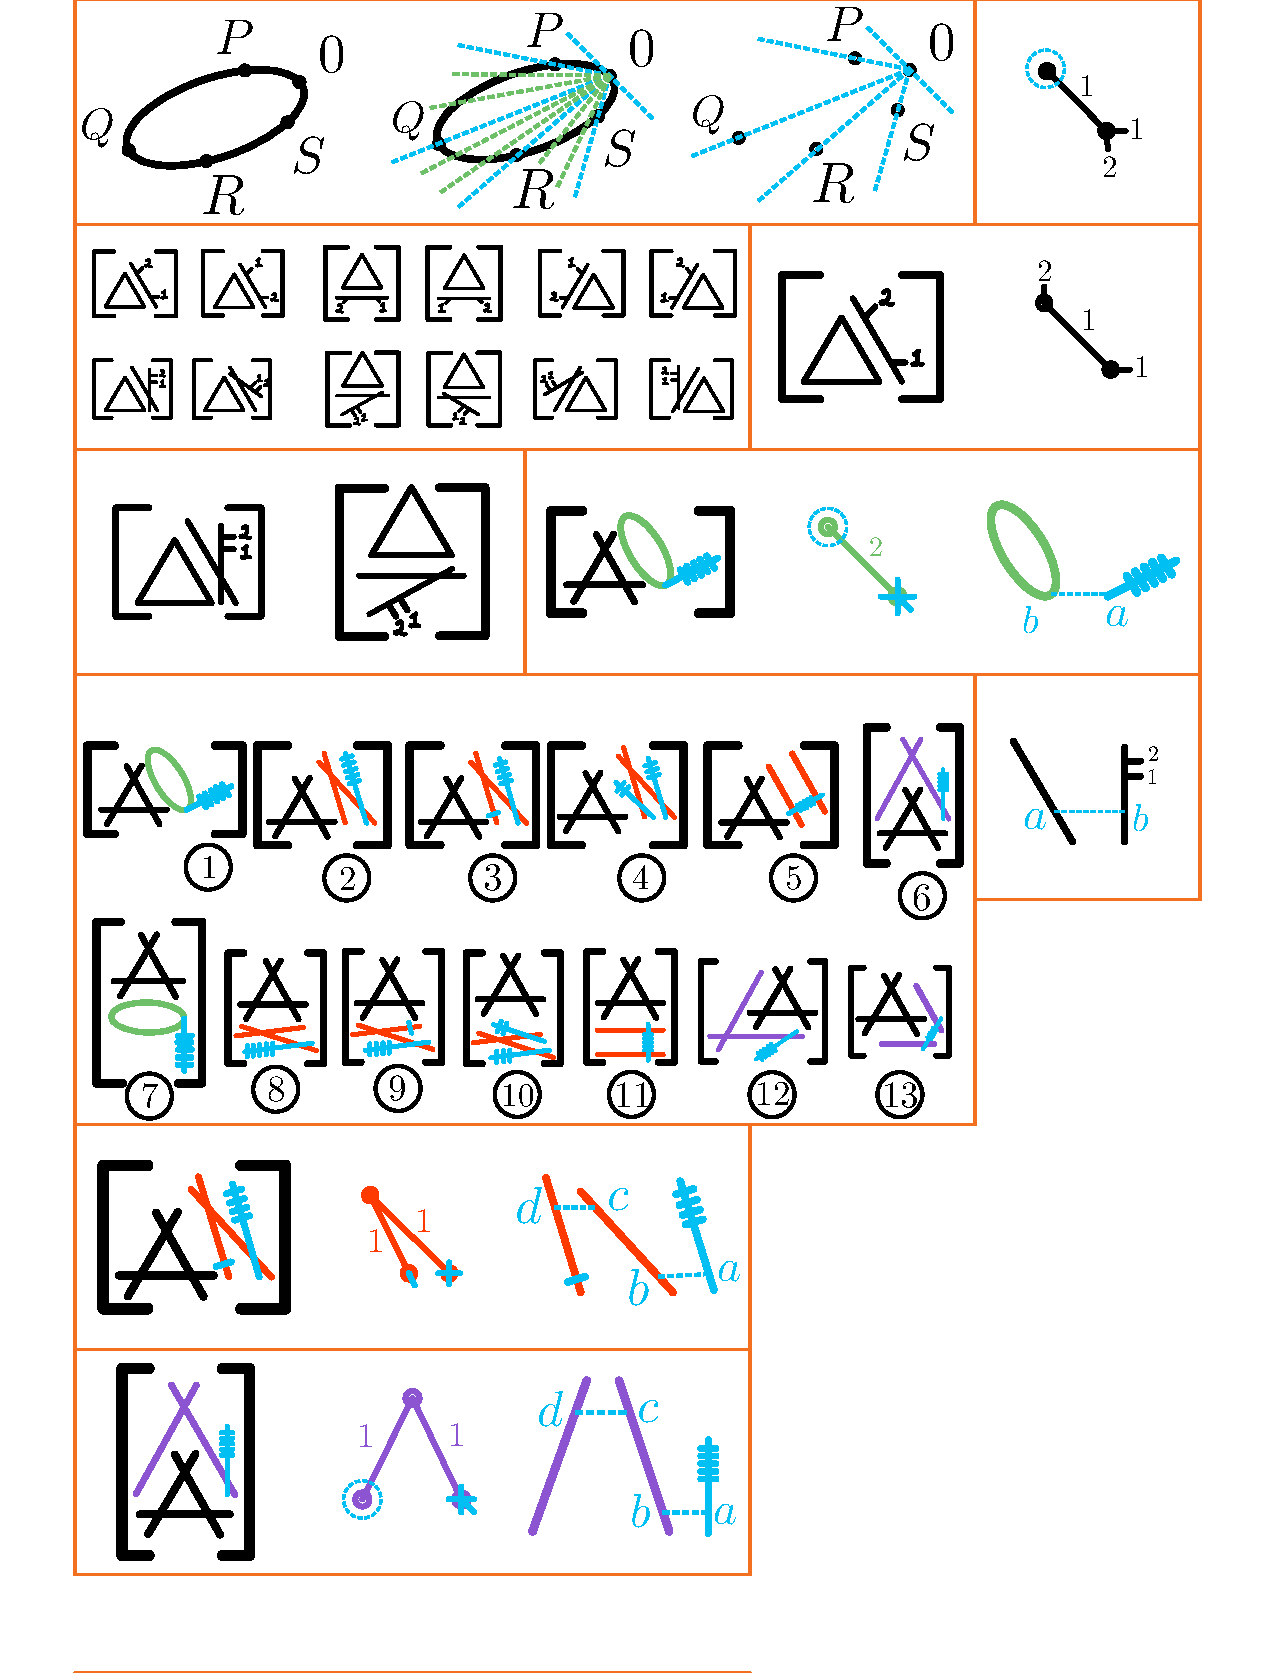
\includegraphics[width=0.9\textwidth, trim= 1.32cm 21cm 9.1cm 4.1cm,clip]{../figs/FigsDNnotability3.pdf}
        \caption{Cohomology classes of the fixed loci $F_1$ through $F_{12}$ of $\ov M_{0,2}(\bP^2,1)$}
        \label{fig:fixed-loci-M02P21}
    \end{figure}
    Via the Atiyah-Bott theorem, we can now express our integral as the sum 
    $$\int_{\ov{M}_{0,2}(\bP^2,1)}\ev_1^\ast([1:0:0])\ev_2^\ast([0:1:0])=\sum_{j=1}^{12}\int_{F_j}\frac{\un i^\ast(\ev_1^\ast([1:0:0])\ev_2^\ast([0:1:0]))}{e(N_{F_j\mid \ov M})}.$$
    express the numerator in easier terms we take advantage of a commutative diagram of inclusions. We will also take the liberty of continuing to abbreviate $\ov{M}_{0,2}(\bP^2,1)$ as $\ov M$ like we did in the normal bundle.
    $$
    \begin{tikzcd}
\bP^2                    & \coprod \pt \arrow[l, "\un i"']                             \\
\ov M \arrow[u, "\ev_i"] & \coprod F_j \arrow[l, "\un i"] \arrow[u, "\ev_{i\mid j}"']
\end{tikzcd}\xrightarrow{H_T^\ast(-)}
\begin{tikzcd}
H^\ast_T(\bP^2) \arrow[d, "\ev_{i}^\ast"'] \arrow[r, "\un i^\ast"] & \bigoplus_{k=1}^3H_T^\ast(\pt) \arrow[d, "\ev_{i\mid j}^\ast"] \\
H_T^\ast(\ov M) \arrow[r, "\un i^\ast"]                            & \bigoplus_{j=1}^{12} H_T^\ast(F_j)                            
\end{tikzcd}
    $$
    The fixed loci of the moduli space represent points, and we know explicitly what the cohomology of a point and projective space from examples \ref{ex:equiv-cohom-point} and \ref{ex-projective-line-cohom-local}. Replacing those into the diagram and leaving the cohomology of the moduli space we obtain the following.
    From this, we can see that taking the route through the point cohomologies into the fixed loci cohomology will provide us with the same result as the one we're taking. Take the point $[1:0:0]$ seen as an equivariant cohomology class in $\bP^2$,
    $$[1:0:0]=(H-t_3)(H-t_2)\xrightarrow{\un i^\ast}(0,(t_1-t_3)(t_1-t_2),0)$$
    and then evaluating via $\ev_{i\mid j}^\ast$ we get 
    $$(p,0,p,0,0,0,p,0,p,0,0,0)\word{where}p=(t_1-t_3)(t_1-t_2).$$
    In the loci where we get zero, the map $\ev_{i\mid j}^\ast$ actually does not exist! This is an artifact of the \emph{empty map} which at the level of cohomology becomes the zero map as the cohomology of the empty set is zero. Similarly for $[0:1:0]$ we have
    $$[0:1:0]=(H-t_3)(H-t_1)\xrightarrow{\un i^\ast}(0,0,(t_2-t_3)(t_2-t_1))$$
    which after mapping through the evaluation gives us 
    $$(q,0,0,0,0,q,0,q,0,0,q,0)\word{where}q=(t_2-t_3)(t_2-t_1).$$
    The integral then can be separated into a sum of 12 terms of which only the first one survives:
    $$I=\int_{F_1}\frac{pq}{e(N_{F_1\mid\ov M})}+\int_{F_2}\frac{0\.q}{e(N_{F_2\mid\ov M})}+\int_{F_3}\frac{p\.0}{e(N_{F_3\mid\ov M})}+\cdots$$
    What remains to be found is the normal bundle to $F_1$ inside the moduli space. Observe that the dimension of this moduli space is 
    $$\dim(\ov M_{0,2}(\bP^2,1))=2+3(1)-1=4$$
    so we expect the normal bundle to a point to have rank 4 and so the Euler class will have degree 4.\par
    To find this normal bundle, we recall the tangent-normal sequence for a point:
    \begin{gather*}
        0\to TF_1\hookto i^\ast T\ov{M}\onto N_{F_1\mid\ov{M}}\to0\\
    \To i^\ast T\ov{M}\isom N_{F_1\mid\ov{M}}
    \end{gather*}
    and the pullback of the tangent bundle becomes the tangent \emph{space} of $\ov M$ at $F_1$. Proceeding from here requires a bit of deformation theory. It happens that the tangent space can be seen as a deformation bundle
    $$T_{F_1}\ov M\isom\DefB(C_1,\un p,\mu_1)$$
    where the curve and map come from the information carried by $F_1$.
    As an element of the moduli space, $F_1$ carries the information of 
    $$F_1=[(C_1,(p_1,p_2),\mu_1)]$$
    so that we may use once again the tangent normal sequence in order to obtain 
    $$0\to TC_1\hookto \mu_1^\ast T\bP^2\onto Q\to 0$$
    where $Q$ is a quotient bundle. Taking the long sequence in cohomology via $H^\ast(C_1,-)$, we get
    \iffalse
    $$
    \begin{tikzcd}
{H^0(C_1,TC_1)} \arrow[r] & {H^0(C_1,\mu_1^\ast T\bP^2)} \arrow[r]\arrow[draw=none]{d}[name=X, anchor=center]{} & {H^0(C_1,Q)}\ar[rounded corners, topath={ -- ([xshift=2ex]\tikztostart.east)|-(X.center)\tikztonodes-|([xshift=-2ex]\tikztotarget.west)--(\tikztotarget)}]{dll}[at end]{\dl} \\
{H^1(C_1,TC_1)} \arrow[r] & {H^1(C_1,\mu_1^\ast T\bP^2)} \arrow[r] & {H^1(C_1,Q)} \\
{H^2(C_1,TC_1)=0}         &                                        &             
\end{tikzcd}
    $$
    \fi
    $$
    \begin{tikzcd}
  H^0(C_1,TC_1) \rar & H^0(C_1,\mu_1^\ast T\bP^2) \rar
             \ar[draw=none]{d}[name=X, anchor=center]{}
    & H^0(C_1,Q) \ar[rounded corners,
            to path={ -- ([xshift=2ex]\tikztostart.east)
                      |- (X.center) \tikztonodes
                      -| ([xshift=-2ex]\tikztotarget.west)
                      -- (\tikztotarget)}]{dll}[at end]{} \\   
 H^1(C_1,TC_1) \rar & H^1(C_1,\mu_1^\ast T\bP^2) \rar
             \ar[draw=none]{d}[name=Y, anchor=center]{}
    & H^1(C_1,Q) \ar[rounded corners,
            to path={ -- ([xshift=2ex]\tikztostart.east)
                      |- (Y.center) \tikztonodes
                      -| ([xshift=-2ex]\tikztotarget.west)
                      -- (\tikztotarget)}]{dll}[at end]{} \\      
  H^2(C_1,TC_1) =0 &\phantom{cuminmyass}&
\end{tikzcd}
$$
In the lens of deformation theory, this sequence becomes
  $$
    \begin{tikzcd}
  \Aut(C_1,\un p)\rar & \DefB(\mu_1) \rar
             \ar[draw=none]{d}[name=X, anchor=center]{}
    & \DefB(C_1,\un p,\mu_1)\ar[rounded corners,
            to path={ -- ([xshift=2ex]\tikztostart.east)
                      |- (X.center) \tikztonodes
                      -| ([xshift=-2ex]\tikztotarget.west)
                      -- (\tikztotarget)}]{dll}[at end]{} \\   
 \DefB(C_1,\un p)\rar & \Ob(\mu_1) \rar
    & \Ob(C_1,\un p,\mu_1) 
\end{tikzcd}
$$
For genus 0, we don't have obstructions (which is a consequence of Serre duality, see \cite{BigMirrorSymmetryBook}, Lemma 24.4.3, pg. 508) so that our sequence becomes 
$$0\to\Aut(C_1,\un p)\to\DefB(\mu_1)\to\DefB(C_1,\un p,\mu_1)\to\DefB(C_1,\un p)\to 0$$
and via a $K$-theory argument we may find the Euler class of the large deformations bundle to be 
$$e(\DefB(C_1,\un p,\mu_1))=\frac{e(\DefB(\mu_1))e(\DefB(C_1,\un p))}{e(\Aut(C_1,\un p))}.$$
It remains on us to find the Euler classes of this particular bundles with respect to $F_1$ in order to express the Euler class of the normal bundle.
\begin{itemize}
    \item The bundle $\Aut(C_1,\un p)$ corresponds to the infinitesimal automorphisms of the curve $C_1$. It is the Lie algebra of the automorphism group of $C_1$. The information which provides us its Euler class is the dual graph of the source curve $C_1$. The Euler class will be the product of the weights of $T\bP^2$ in the points where the valence 1 vertices map to.
    \begin{figure}[h!]
        \centering
        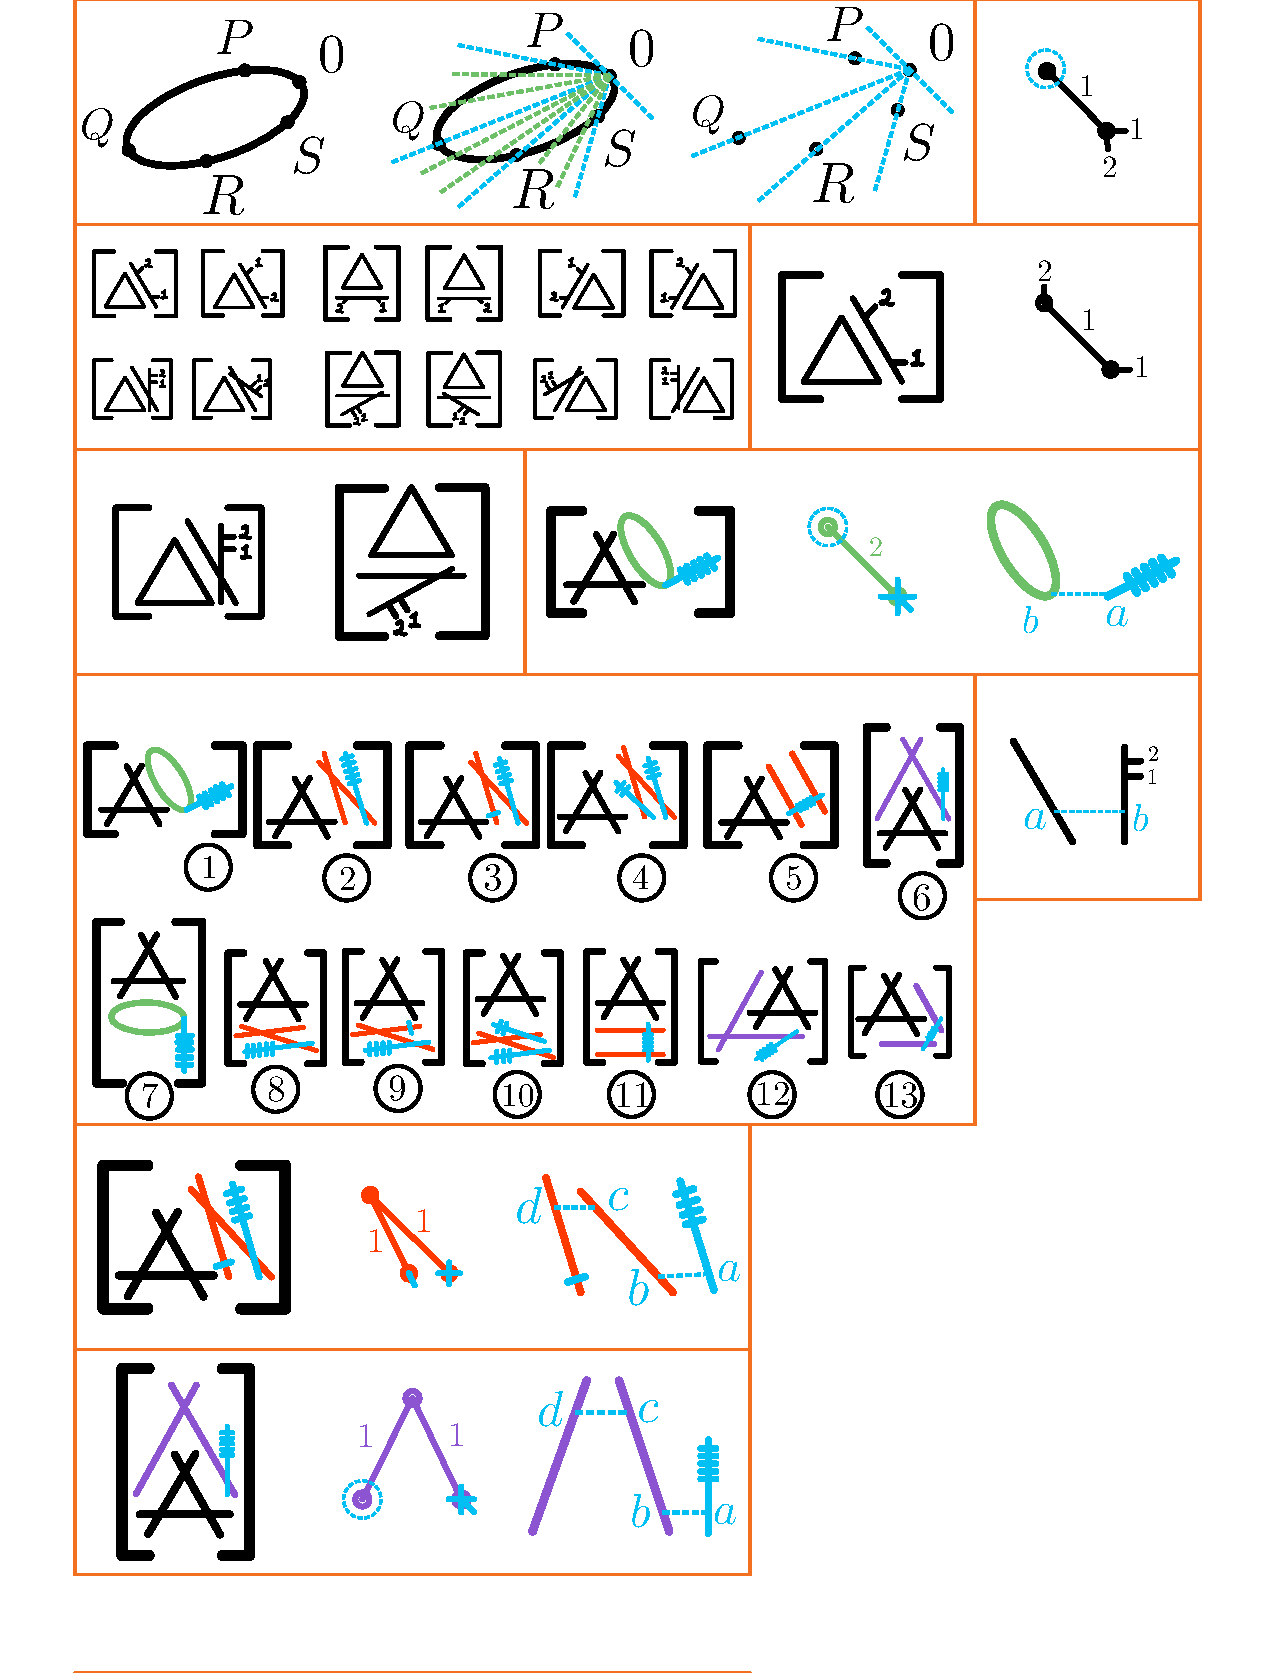
\includegraphics[width=0.5\textwidth, trim= 12.9cm 21cm 1.5cm 4.1cm,clip]{../figs/FigsDNnotability3.pdf}
        \caption{Fixed loci $F_1$ along the dual graph of $C_1$}
        \label{fig:F1-and-C1-dual-graph}
    \end{figure}
    From the graph we may see that there's no valence 1 vertices so that there's no automorphisms. Hence, 
    $$e(\Aut(C_1))=0$$
    and even if it appears we are dividing by zero, we are not. This will cancel out further along the way.
    \item For $\DefB(C_1,\un p)$ we look at the normalization of the curve $C_1$. However since our curve is smooth, the normalization is itself and we cannot find points which map into a node. These points are the ones which contribute to the Euler class. Once again, the result is zero and this cancels out with $e(\Aut(C_1,\un p))$.
    \item Finally, recall 
    $$\DefB(\mu_1)\isom  H^0(C_1,\mu_1^\ast T\bP^2).$$
    This is an equivariant line bundle which decomposes as 
    $$T\bP^2\isom T\set{Z=0}\oplus N_{\set{Z=0}\mid\bP^2}\isom\cO(2)\oplus\cO(1).$$
    The Euler class is then a product of the Euler classes of these bundles which are $1^{\text{st}}$ Chern classes, as they're line bundles. Observe that when restricting for example the normal bundle to $p_1$ and $p_2$ we have 
    $$c_1(N_{\mid p_1})=t_1-t_3,\word{and}c_1(N_{\mid p_2})=t_2-t_3.$$
    In a similar fashion, the weights of the tangent bundle are $t_1-t_2$ and $t_2-t_1$ respectively. We conclude that 
    $$e(\DefB(\mu_1))=(t_1-t_3)(t_2-t_3)(t_1-t_2)(t_2-t_1).$$
\end{itemize}
Summarizing we have 
$$e(N_{F_1\mid\ov M})=\frac{0\.(t_1-t_3)(t_2-t_3)(t_1-t_2)(t_2-t_1)}{0}=(t_1-t_3)(t_2-t_3)(t_1-t_2)(t_2-t_1).$$
Observe that the degree of the Euler class is 4 as expected.
The integral is finally 
$$I=\int_{F_1}\frac{pq}{e(N_{F_1\mid\ov M})}=\int_{F_1}\frac{(t_1-t_3)(t_1-t_2)(t_2-t_3)(t_2-t_1)}{(t_1-t_3)(t_2-t_3)(t_1-t_2)(t_2-t_1)}=\int_{F_1}1=1.$$
This confirms that, indeed, the number of lines passing through 2 points in the plane is precisely 1.
\end{Ex} 

This example didn't illustrate the full calculation of deformation and automorphism bundles. We can still enjoy the moduli space we're working in to do the same calculation but now instead asking for the integral of 
$$\ev_1^\ast([1:0:0])\ev_2^\ast([1:0:0])$$
requiring us to consider loci mapping both marks to the same point $[1:0:0]$. This should produce the same result but only considering a different procudure.

\begin{Ex}
    Let us find 
    $$\int_{\ov{M}_{0,2}(\bP^2,1)}\prod_{i=1}^{2}\ev_i^\ast([1:0:0]).$$
    We know that loci such that $p_1$ is mapped to $[1:0:0]$ are $F_1,F_3,F_7$ and $F_9$. While those such that $p_2$ maps there are $F_2,F_4,F_7$ and $F_9$. Thus the fixed loci which take $p_1$ and $p_2$ both to $[1:0:0]$ are $F_7$ and $F_9$.
    \begin{figure}[h!]
        \centering
        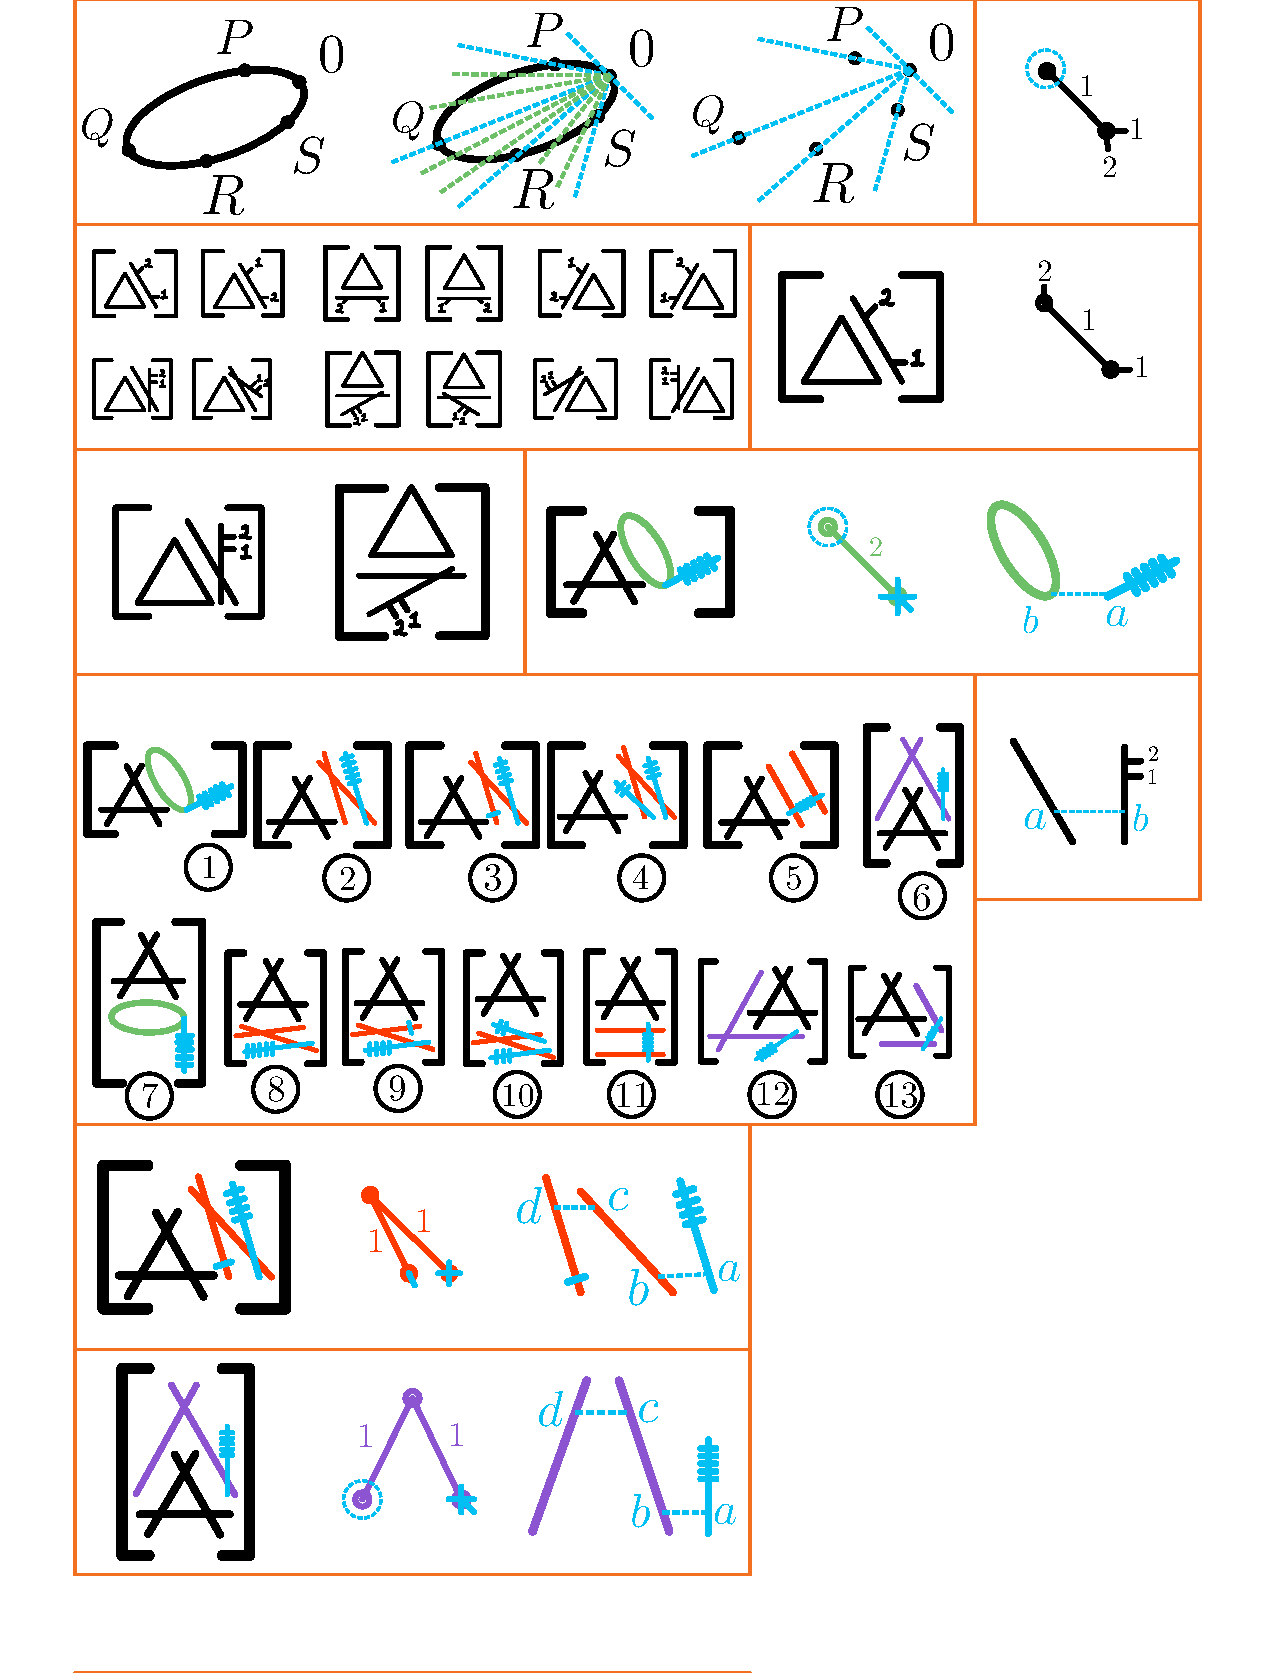
\includegraphics[width=0.45\textwidth, trim= 1.32cm 17cm 13.1cm 8cm,clip]{../figs/FigsDNnotability3.pdf}
        \caption{Fixed loci $F_7$ and $F_9$}
        \label{fig:fixed-loci-M02P21-F7-F9}
    \end{figure}
    The integral becomes 
    $$I=\int_{F_7}\frac{p^2}{e(N_{F_7\mid\ov M})}+\int_{F_9}\frac{p^2}{e(N_{F_9\mid\ov M})},\word{where}p=(t_1-t_3)(t_2-t_3)$$
    and once again we're left with finding the normal bundles. Observe that we only need to find one as the other is obtained by transposing $[0:1:0]$ with $[0:0:1]$. In terms of the Euler class, it'll be sufficient to say 
    $$e(N_{F_9\mid\ov M})=(23)\.e(N_{F_7\mid\ov M})$$
    where the permutation acts on the variables.
    \begin{itemize}
        \item The dual graph of $C_7$ has one vertex of valence 1. This corresponds to a point mapping to $[0:1:0]$. Thus this acquires a tangent weight in the direction of the line which maps to $Z=0$.
        \begin{figure}[h!]
        \centering
        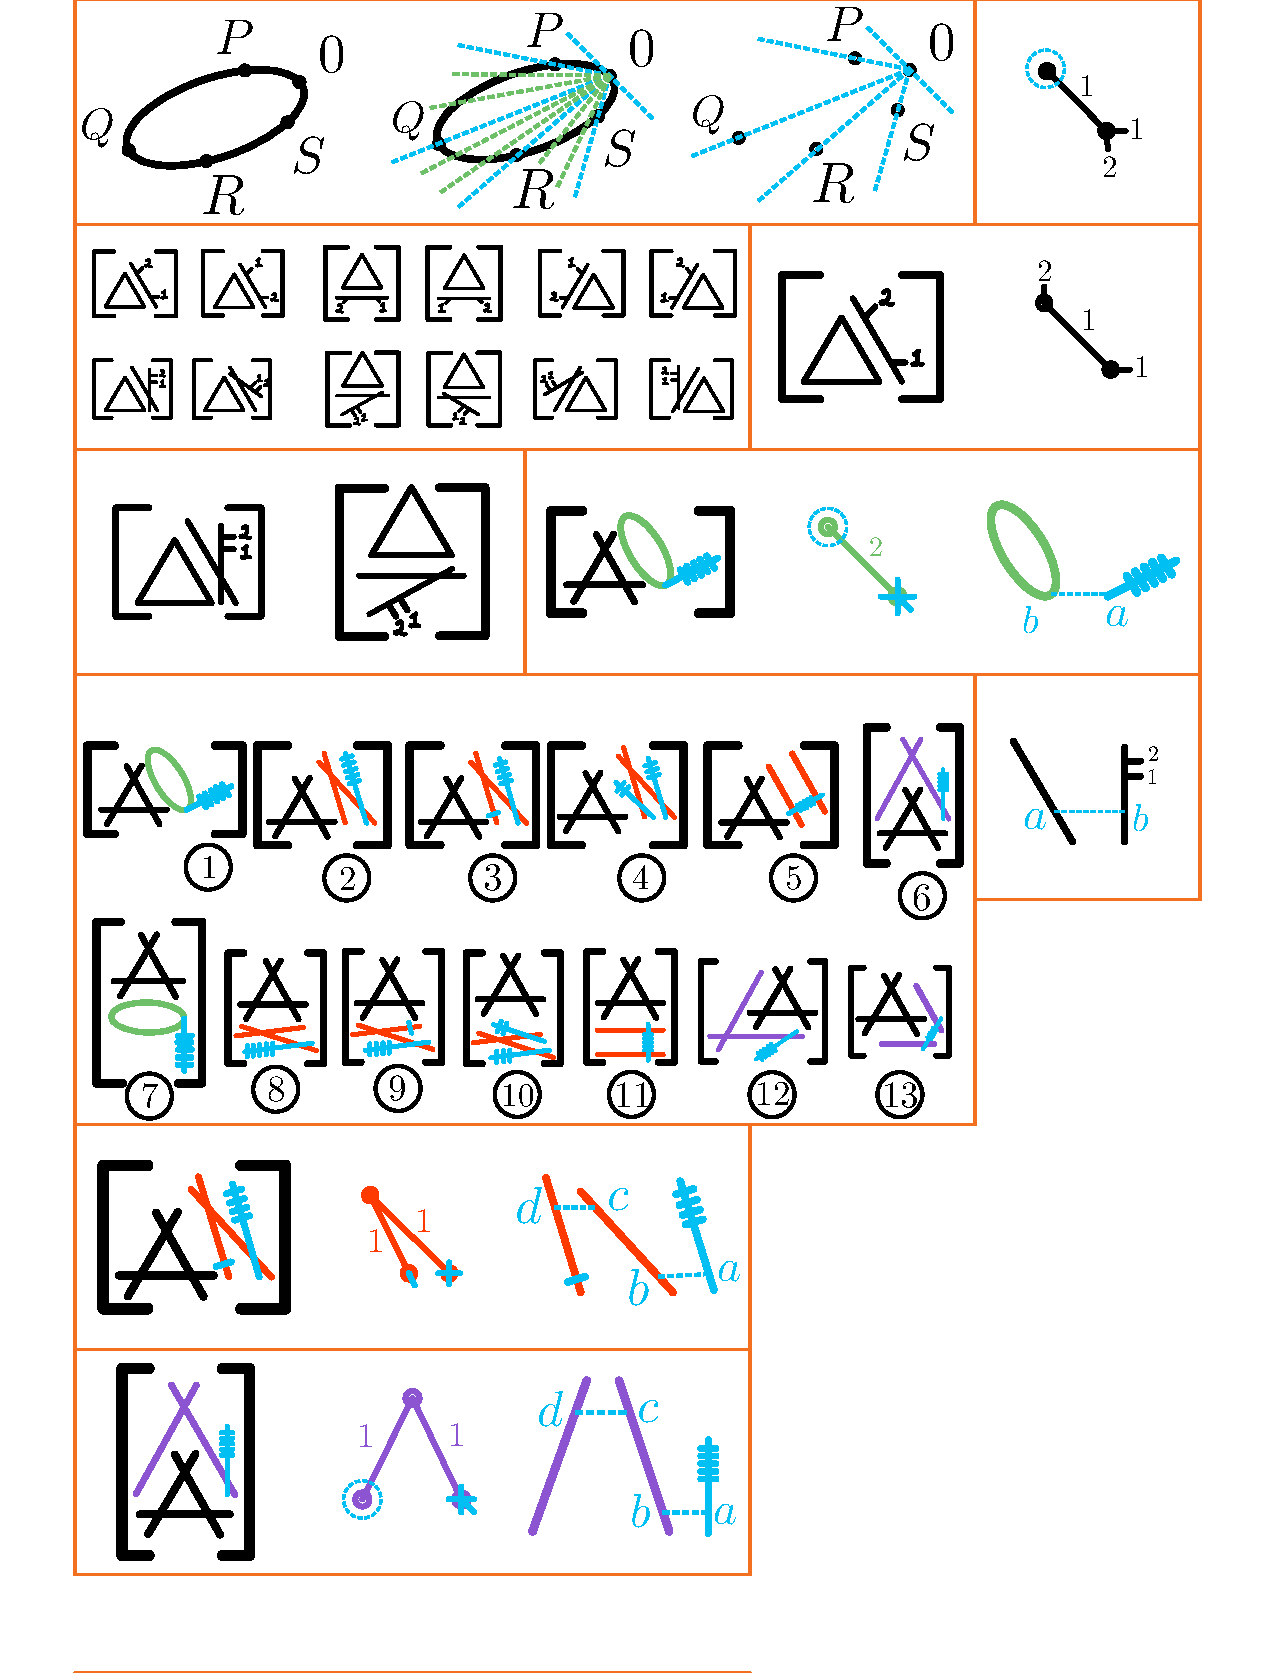
\includegraphics[width=0.2\textwidth, trim= 17cm 25.3cm 2cm 0.8cm,clip]{../figs/FigsDNnotability3.pdf}
        \caption{Dual graph of $C_7$}
        \label{fig:dual-graph-nodal-M02P21}
    \end{figure}
        We obtain 
        $$e(\Aut(C_7))=t_2-t_1.$$
        \item The curve now has a node and can be normalized. Let us call $a$ and $b$ the points mapping to the node.
             \begin{figure}[h!]
        \centering
        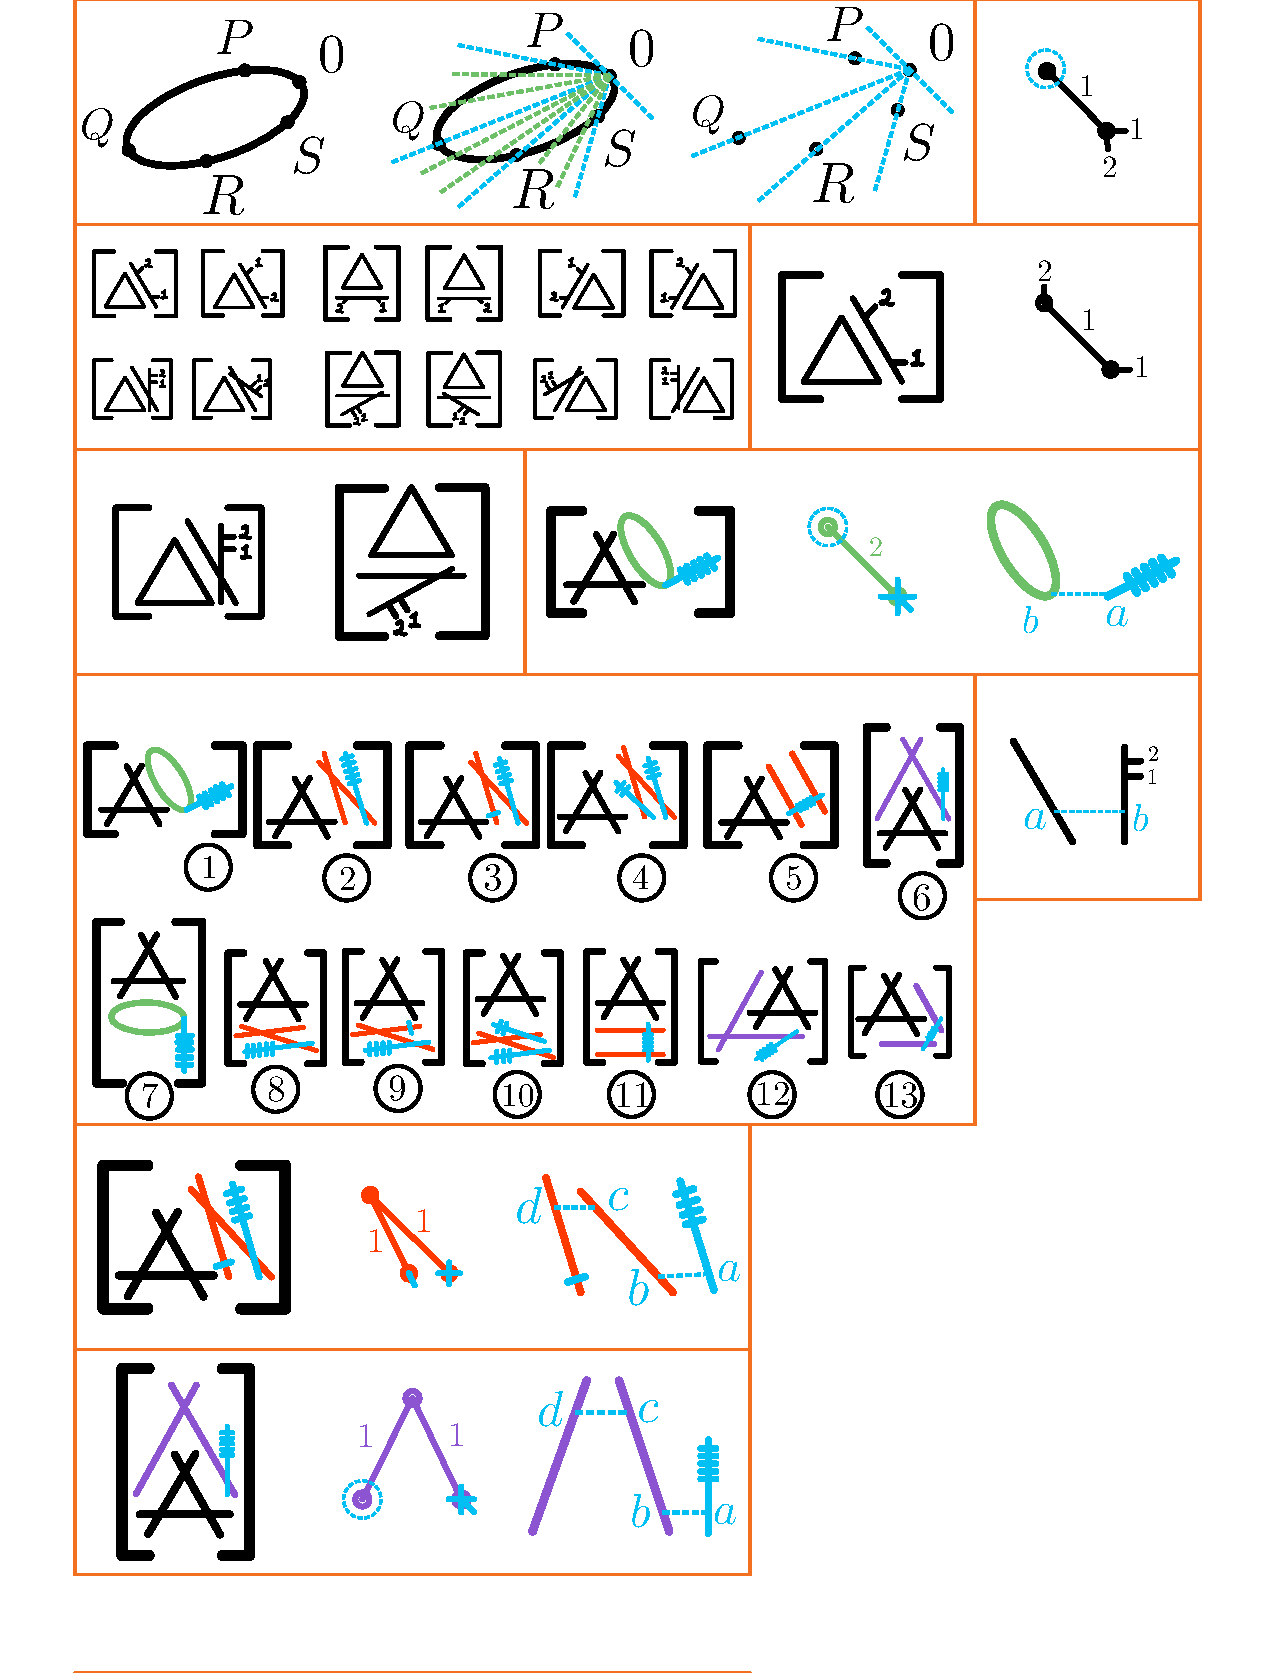
\includegraphics[width=0.2\textwidth, trim= 17cm 14cm 2cm 12.5cm,clip]{../figs/FigsDNnotability3.pdf}
        \caption{Normalization of $C_7$ with $a,b$ mapping to the node.}
        \label{fig:normalization-nodal-M02P21}
    \end{figure}
        We have 
        $$e(\DefB(C_7))=(-\psi_a-\psi_b)$$
        where $-\psi_a$ corresponds to the tangent weight of the point mapping to $[1:0:0]$ and $\psi_b$ is a psi-class on $M_{0,3}$. This turns out to be zero so that 
        $$e(\DefB(C_7))=((t_1-t_2)+0)=t_1-t_2.$$
        \item In order to compute the deformations of the map, we look at the normalization sequence of $C_7$. The sequence of sheaves is 
        $$0\to\cO_{C_7}\to\cO_{C_{7,1}}\oplus\cO_{C_{7,2}}\to\un\bC_{n}\to0,$$
        where each component of the normalization gets a structure sheaf and each node, a skyscraper. Tensoring the sequence by $-\ox \mu_7^\ast\cO(d)$ $(d=1,2)$, and taking cohomology $H^\ast(C,-)$ we get two sequences:
        \begin{gather*}
            0\to H^0(C_7,\mu_7^\ast\cO(1))\to\genr{1,x}\oplus\genr{1}\to\genr{1}\to 0,\\
            0\to H^0(C_7,\mu_7^\ast\cO(2))\to\genr{1,x,x^2}\oplus\genr{1}\to\genr{1}\to 0.
        \end{gather*}
        We must be appreciative of the fact that there's not a second line of first cohomologies due to the fact that we're working on genus zero. This is justified due to Serre duality. But in anyhow, the Euler class of $H^0(C_7,\mu_7^\ast\cO(d))$ is then the product of the terms right next divided by those furthest away from it. We have thus 
        \begin{gather*}
        e(H^0(C_7,\mu_7^\ast\cO(1)))=\frac{(t_2-t_3)(t_1-t_3)(t_1-t_3)}{t_1-t_3}=(t_2-t_3)(t_1-t_3)\\
        e(H^0(C_7,\mu_7^\ast\cO(2)))=\frac{(t_2-t_1)(t_1-t_2)(t_1-t_2)}{t_1-t_2}=(t_2-t_1)(t_1-t_2)
        \end{gather*}
        and the $x$ term has no weight as it corresponds to a fixed weight of the action.
    \end{itemize}
     From this
        \begin{align*}
             e(N_{F_7\mid\ov M})&=\frac{[(t_2-t_3)(t_1-t_3)(t_2-t_1)(t_1-t_2)][t_1-t_2]}{t_2-t_1}\\
             &=(t_1-t_2)^2(t_1-t_3)(t_2-t_3)
        \end{align*}
    and immediately
    $$e(N_{F_9\mid\ov M})=(t_1-t_3)^2(t_1-t_2)(t_3-t_2).$$
    We conclude once again that 
    $$I=\int_{\pt}\left(\frac{((t_1-t_3)(t_1-t_2))^2}{(t_1-t_2)^2(t_1-t_3)(t_2-t_3)}+\frac{((t_1-t_3)(t_1-t_2))^2}{(t_1-t_2)^2(t_1-t_3)(t_2-t_3)}\right)=\int_{\pt}1=1,$$
    confirming once again that the number of lines through two points in the plane is 1.
\end{Ex}

Similar to this calculation in the sense that nodal curves appear, we will find such curves when calculating $N_2$, for example. The number of conics passing through $5$ points is famously known to be $1$. This number can be calculated as another integral.

\begin{Ex}
We will calculate 
    $$\int_{\ov{M}_{0,5}(\bP^2,2)}\prod_{i=1}^{5}\ev_i^\ast([1:0:0]).$$
    The torus action on this space of maps has quite a bunch of fixed loci, so instead of indicating all the fixed loci and then looking at which ones map all 5 points to $[1:0:0]$, we will instead enumerate such fixed loci.
    \begin{figure}[h!]
        \centering
        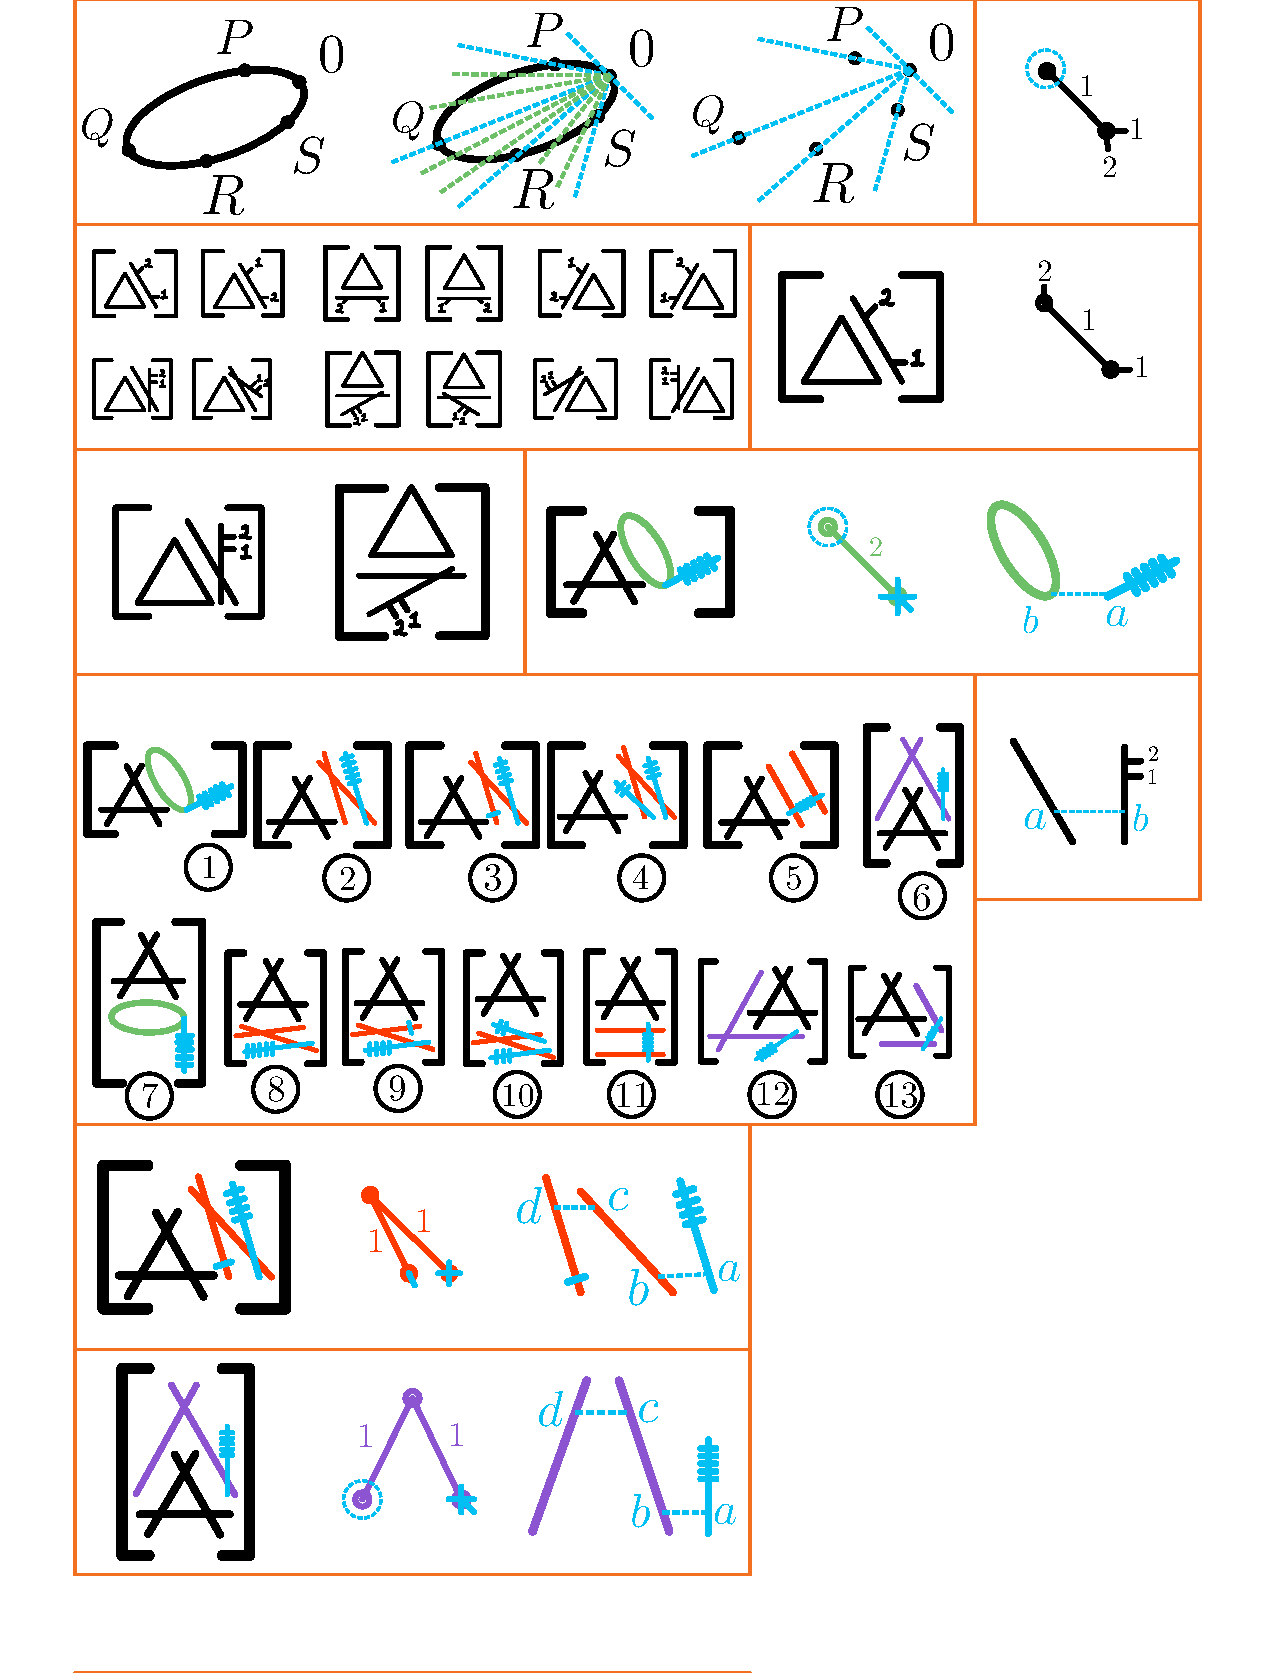
\includegraphics[width=0.9\textwidth, trim= 1.32cm 9.4cm 5.2cm 12.1cm,clip]{../figs/FigsDNnotability3.pdf}
        \caption{Fixed loci of $\ov M_{0,5}(\bP^2,2)$ mapping $5$ marks to $[1:0:0]$}
        \label{fig:fixed-loci-M05P22-100}
    \end{figure}
    Observe that we have not labeled the marks on the curve so that we must count the possible different labels on the curve. For example in $F_3$, there's $\binom{5}{1}$ ways to arrange a mark on one side and the other $4$ on the other side.\par
    Notice also that reflecting by the bisector passing through $[1:0:0]$ we get from loci $F_j$, $F_{j+6}$ for $j\in[6]$. We thus require to only calculate the integrals over $F_1,\dots,F_6$ and $F_{13}$. Let us explain the calculation for $F_1$, $F_3$, $F_6$ and $F_{13}$, the rest are analogous and we summarize in a table after this calculations.\par
    Consider the fixed loci $F_1$, along its dual graph and the normalization of the curve $C_1$.
    \begin{figure}[h!]
        \centering
        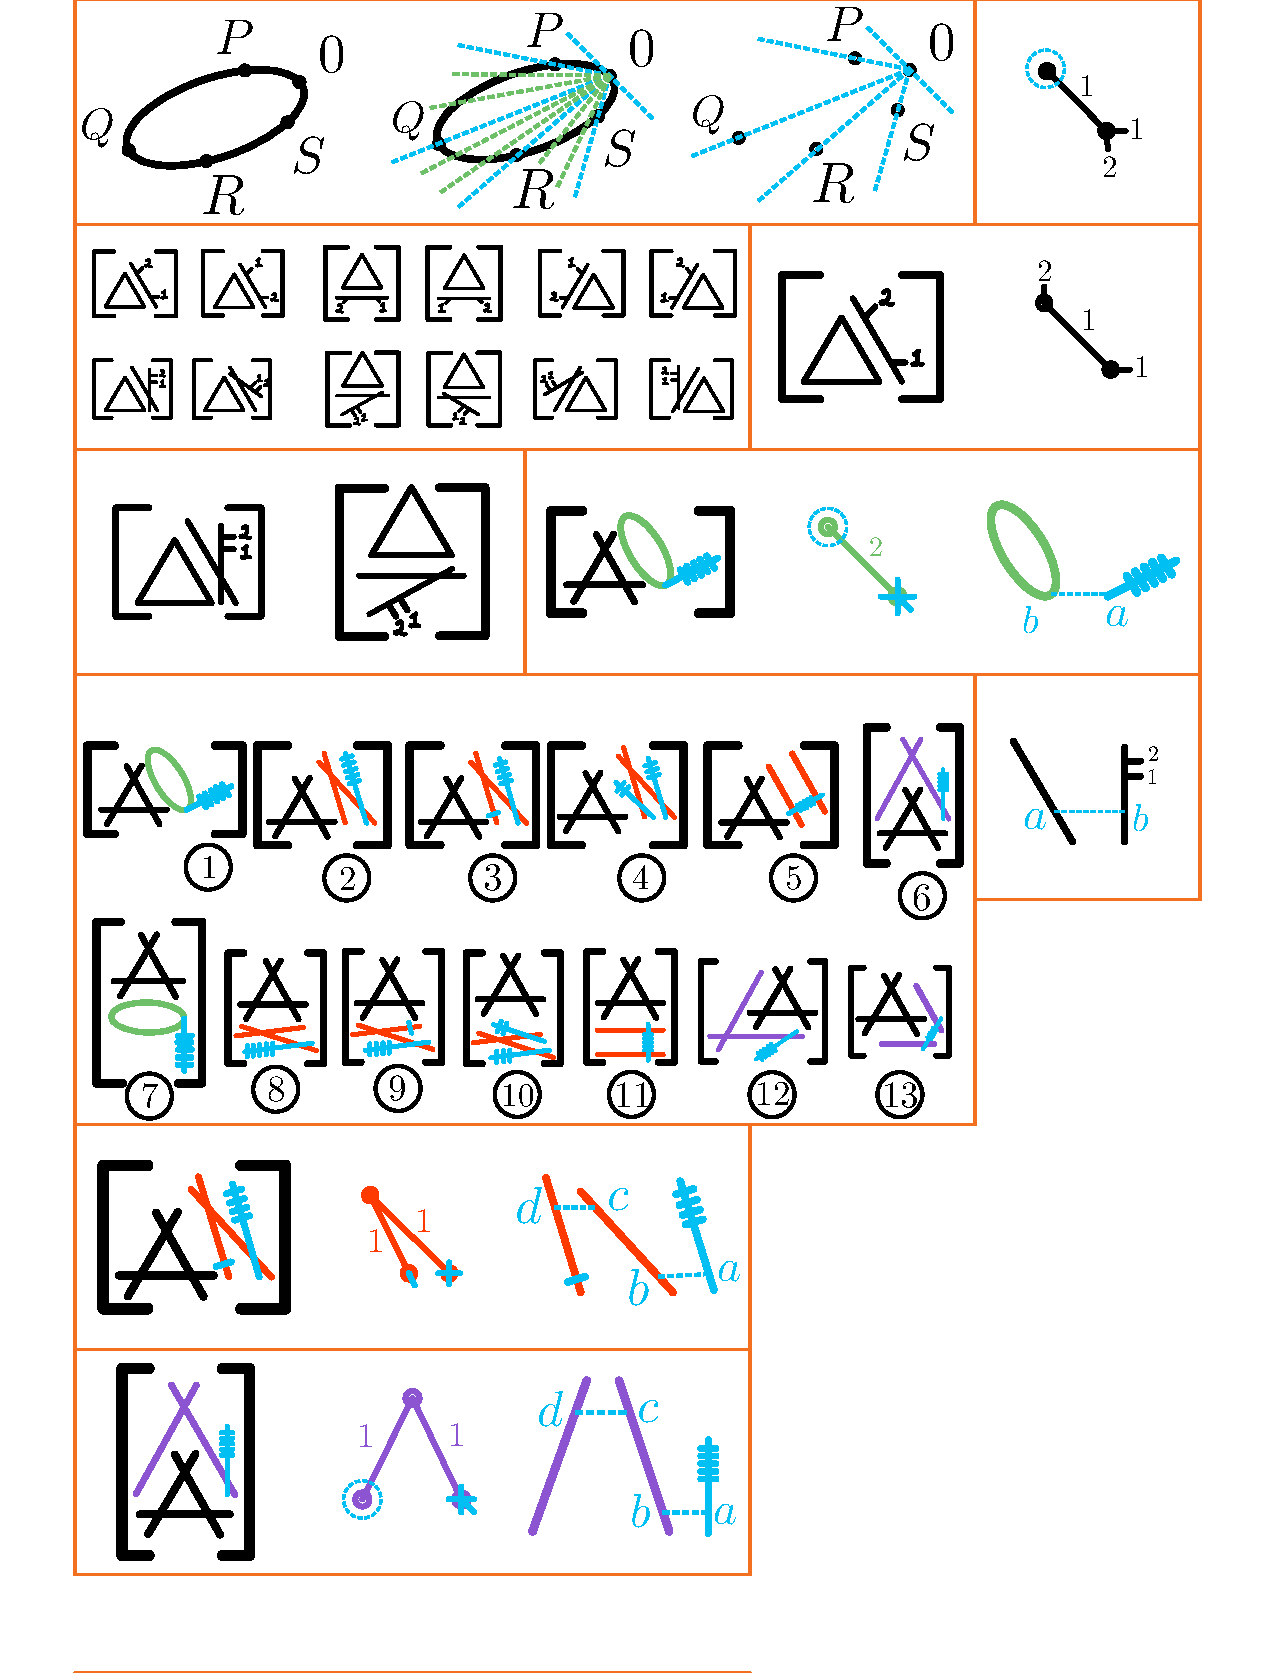
\includegraphics[width=0.7\textwidth, trim= 9cm 17cm 1.3cm 8cm,clip]{../figs/FigsDNnotability3.pdf}
        \caption{Double cover of $\set{Z=0}$ with dual graph and normalization of source curve}
        \label{fig:double-cover-F1-5marks}
    \end{figure}
    \begin{itemize}
        \item For $\Aut(C_1)$, we look at the vertex of valence $1$. This contributes the weight of the point where it maps to. \emph{However} as the map has degree $2$, we must divide the weight by $2$. This means that 
        $$e(\Aut(C_1))=\half(t_2-t_1).$$
        \item Observing the normalization of the curve allows us to see that there's two points $a,b$ mapping to a node. From that, 
        $$e(\DefB(C_1))=(-\psi_a-\psi_b)$$
        and the value of $-\psi_a$ is $\half(t_1-t_2)$ as it corresponds to the tangent weight of the point where $a$ maps to. This means that 
        $$e(\DefB(C_1))=\left(\half(t_1-t_2)-\psi_b\right)=\half(t_1-t_2)\left(1-\frac{2\psi_b}{t_1-t_2}\right)$$
        whereas $\psi_b$ is a psi-class on a copy of $\ov{M}_{0,6}$. This will be integrated in the end to a rational function in terms of $t_i$'s.
        \item Now looking for $e(\DefB(\mu_1))$, we must use the normalization sequence of $C_1$. Consider the sequence 
        $$0\to\cO_{C_1}\to\cO_{C_{1,1}}\oplus\cO_{C_{1,2}}\to\un\bC_{n}\to0$$
        where $C_{1,1}$ is the non-contracted component and $C_{1,2}$ the one which contracts. We tensor the sequence by $-\ox \mu_1^\ast\cO(d)$ $(d=1,2)$ and take cohomology $H^\ast(C,-)$ to get two sequences:
        \begin{gather*}
            0\to H^0(C_1,\mu_1^\ast\cO(1))\to\genr{1,x,x^2}\oplus\genr{1}\to\genr{1}\to 0,\\
            0\to H^0(C_1,\mu_1^\ast\cO(2))\to\genr{1,x,x^2,x^3,x^4}\oplus\genr{1}\to\genr{1}\to 0.
        \end{gather*}
        Observe that in this case the $\cO(d)$ pulls-back as an $\cO(2d)$ bundle because of the degree of $\mu_1$. From this, the weights of $\cO(d)$ bundles do pullback as usual but the middle weights change. We have that 
        \begin{align*}
        e(H^0(C_1,\mu_1^\ast\cO(1)))&=\frac{(t_1-t_3)(t_1-t_3-\half(t_1-t_2))(t_2-t_3)(t_1-t_3)}{t_1-t_3}\\
        &=\half(t_1-t_3)\left(t_1+t_2-2t_3\right)(t_2-t_3)\\
        e(H^0(C_1,\mu_1^\ast\cO(2)))&=\frac{t_1-t_2}{t_1-t_2}\sum_{\substack{k=0\\ k\neq 2}}^{4}\left(t_1-t_2-\frac{k}{2}(t_1-t_2)\right)\\
        &=\frac{1}{4}(t_1-t_2)^4
        \end{align*}
        and the $x^2$ would correspond with the $t_1-t_2-\frac{2}{2}(t_1-t_2)$ term, but as that is fixed by the action, it does not contribute to the final value of the Euler class.
        Finally we have that 
        $$e(\DefB(\mu_1))=\frac{1}{8}(t_1-t_2)^4(t_1-t_3)(t_2-t_3)\left(t_1+t_2-2t_3\right).$$
    \end{itemize}
    Combining this together into the whole Euler class we find that 
    \begin{align*}
    e(N_{F_1\mid\ov M})&=\frac{\bonj{\frac{1}{8}(t_1-t_2)^4(t_1-t_3)(t_2-t_3)\left(t_1+t_2-2t_3\right)}\bonj{\half(t_1-t_2)\left(1-\frac{2\psi_b}{t_1-t_2}\right)}}{\half(t_2-t_1)}\\
    &=-\frac{1}{8}(t_1-t_2)^4(t_1-t_3)(t_2-t_3)\left(t_1+t_2-2t_3\right)\left(1-\frac{2\psi_b}{t_1-t_2}\right)
    \end{align*}
    which has degree $7$. This corresponds with the codimension of $\ov{M}_{0,6}$ with respect to $\ov M_{0,5}(\bP^2,2)$ which is $5+3(2)-1=10$.\par
    Integrating we see that
    \begin{align*}
        I_1&=\int_{F_1}\frac{p^5}{e(N_{F_1\mid\ov M})}\\
        &=\int_{\ov M_{0,6}}\frac{(t_1-t_3)^5(t_1-t_2)^5}{-\frac{1}{8}(t_1-t_2)^4(t_1-t_3)(t_2-t_3)\left(t_1+t_2-2t_3\right)\left(1-\frac{2\psi_b}{t_1-t_2}\right)}\\
        &=\frac{-8(t_1-t_3)^4(t_1-t_2)}{(t_2-t_3)\left(t_1+t_2-2t_3\right)}\int_{\ov M_{0,6}}\frac{1}{1-\frac{2\psi_b}{t_1-t_2}}\\
        &=\frac{-8(t_1-t_3)^4(t_1-t_2)}{(t_2-t_3)\left(t_1+t_2-2t_3\right)}\int_{\ov M_{0,6}}\sum_{k=0}^{\infty}\left(\frac{2\psi_b}{t_1-t_2}\right)^k\\
        &=\frac{-8(t_1-t_3)^4(t_1-t_2)}{(t_2-t_3)\left(t_1+t_2-2t_3\right)}\left(0+\dots+\int_{\ov M_{0,6}}\left(\frac{2\psi_b}{t_1-t_2}\right)^3+0+\dots\right)\\
        &=\frac{-64(t_1-t_3)^4}{(t_1-t_2)^2(t_2-t_3)\left(t_1+t_2-2t_3\right)}\int_{\ov M_{0,6}}\psi_b^3\\
        &=\frac{-64(t_1-t_3)^4}{(t_1-t_2)^2(t_2-t_3)\left(t_1+t_2-2t_3\right)}
    \end{align*}
    where we have used the string equation to find the value of the integral in the end. There's one more thing to do which is divide by $2$ the whole integral as this loci is actually a stacky $\half\ov{M}_{0,6}$ so that in the end
    $$I_1=\frac{-32(t_1-t_3)^4}{(t_1-t_2)^2(t_2-t_3)\left(t_1+t_2-2t_3\right)}.$$
    Let us proceed with $F_3$, we must look at its dual graph and the normalization of $C_3$. 
    \begin{figure}[h!]
        \centering
        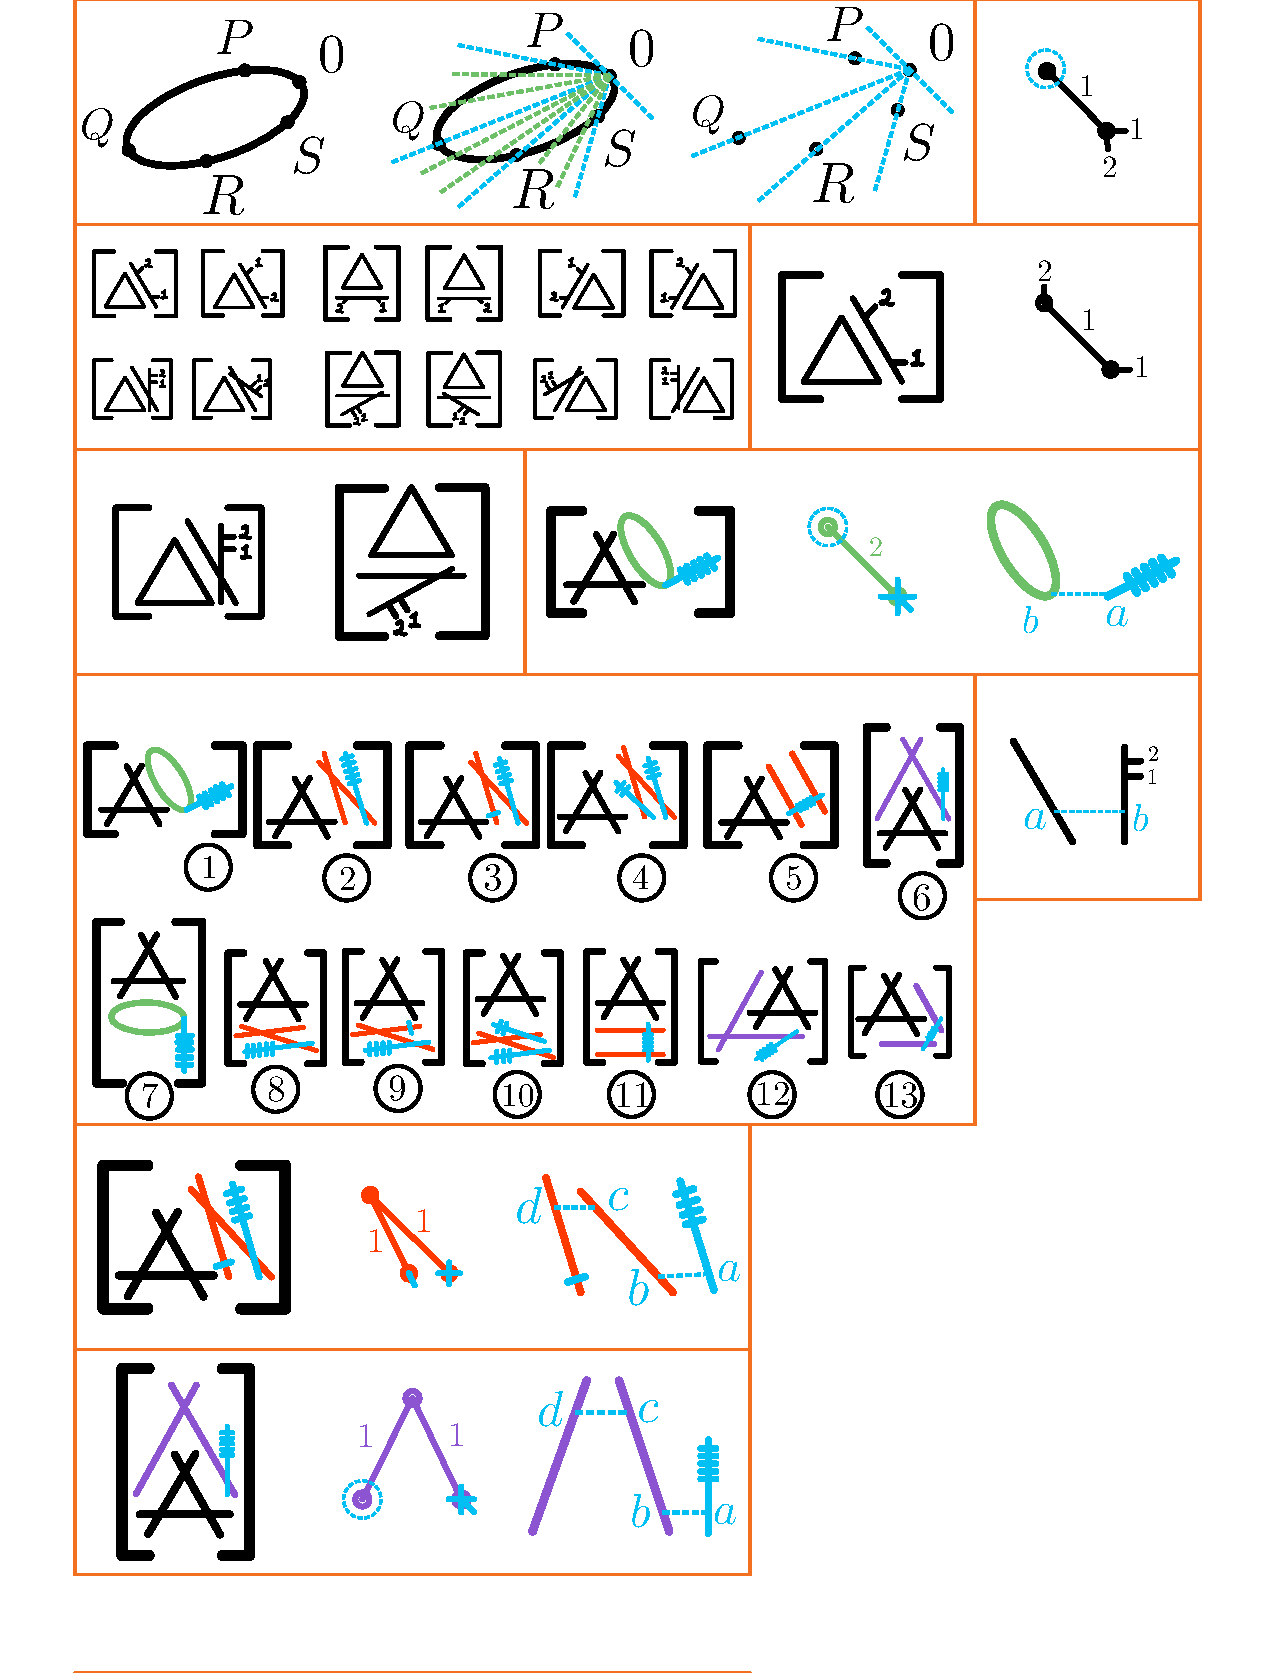
\includegraphics[width=0.7\textwidth, trim= 1.32cm 5.6cm 9cm 19.5cm,clip]{../figs/FigsDNnotability3.pdf}
        \caption{Loci $F_3$ along dual graph and normalization of source curve}
        \label{fig:quadratic-F3-5-marks}
    \end{figure}
    \begin{itemize}
        \item The dual graph of $C_3$ has no vertex of valence $1$ so that $e(\Aut(C_3))=0$.
        \item We have 4 points $a,b,c$ and $d$ which map to two nodes. Each of these contributes a negative psi-class so that 
        \begin{align*}
            e(\DefB(C_3))&=(-\psi_a-\psi_b)(-\psi_c-\psi_d)\\
            &=(-\psi_a+(t_1-t_2))((t_2-t_1)+(t_2-t_1))\\
            &=-2(t_1-t_2)^2\left(1-\frac{\psi_a}{t_1-t_2}\right)
        \end{align*}
        where the psi-class $\psi_a$ belongs to the corresponding $\ov{M}_{0,5}$ component. The other psi-classes correspond to the tangent weights of the points where their respective point maps to.
        \item Finally the normalization sequence for $C_3$ is 
        $$0\to\cO_{C_3}\to\cO_{C_{3,1}}\oplus\cO_{C_{3,2}}\oplus\cO_{C_{3,3}}\to\un\bC_{n_1}\oplus\un\bC_{n_2}\to 0$$
        which we tensor by $-\ox \mu_1^\ast\cO(d)$ $(d=1,2)$ and then take cohomology $H^\ast(C,-)$ to get two sequences:
        \begin{gather*}
            0\to H^0(C_3,\mu_3^\ast\cO(1))\to\genr{1,x}\oplus\genr{1,x}\oplus\genr{1}\to\genr{1}\oplus\genr{1}\to 0,\\
            0\to H^0(C_3,\mu_3^\ast\cO(2))\to\genr{1,x,x^2}\oplus\genr{1,x,x^2}\oplus\genr{1}\to\genr{1}\oplus\genr{1}\to 0.
        \end{gather*}
        We obtain the respective Euler classes which we multiply to get the full Euler class for the deformation bundle:
        \begin{align*}
        e(H^0(C_3,\mu_3^\ast\cO(1)))&=\frac{(t_1-t_3)(t_2-t_3)(t_2-t_3)(t_1-t_3)(t_1-t_3)}{(t_2-t_3)(t_1-t_3)}\\
        &=(t_1-t_3)^2(t_2-t_3)\\
        e(H^0(C_3,\mu_3^\ast\cO(2)))&=\frac{(t_1-t_2)(t_2-t_1)(t_2-t_1)(t_1-t_2)(t_1-t_2)}{(t_2-t_1)(t_1-t_2)}\\
        &=-(t_1-t_2)^3\\
        \To e(\DefB(\mu_3))&=-(t_1-t_2)^3(t_1-t_3)^2(t_2-t_3)
        \end{align*}
    \end{itemize}
    Finally the Euler class for $N_{F_3\mid\ov M}$ is 
    \begin{align*}
        e(N_{F_3\mid\ov M})&=\bonj{-(t_1-t_2)^3(t_1-t_3)^2(t_2-t_3)}\bonj{-2(t_1-t_2)^2\left(1-\frac{\psi_a}{t_1-t_2}\right)}\\
        &=2(t_1-t_2)^5(t_1-t_3)^2(t_2-t_3)\left(1-\frac{\psi_a}{t_1-t_2}\right)
    \end{align*}
    which has degree 8 as the codimension of $\ov M_{0,5}$ in $\ov M_{0,5}(\bP^2,2)$. The whole resulting integral is then 
    \begin{align*}
        I_3&=\int_{F_3}\frac{p^5}{e(N_{F_3\mid\ov M})}\\
        &=\int_{\ov M_{0,5}}\frac{(t_1-t_3)^5(t_1-t_2)^5}{2(t_1-t_2)^5(t_1-t_3)^2(t_2-t_3)\left(1-\frac{\psi_a}{t_1-t_2}\right)}\\
        &=\frac{(t_1-t_3)^3}{2(t_2-t_3)}\int_{\ov M_{0,5}}\frac{1}{1-\frac{\psi_a}{t_1-t_2}}\\
        &=\frac{(t_1-t_3)^3}{2(t_1-t_2)^2(t_2-t_3)}\int_{\ov M_{0,5}}\psi_a^2\\
        &=\frac{(t_1-t_3)^3}{2(t_1-t_2)^2(t_2-t_3)}.
    \end{align*}
    However, observe that the order in which we chose the marks plays no r\^ole into the calculation of this integral. We thus add a factor of $\binom{5}{1}$ accounting for the distribution of the marks in order to get 
    $$I_3=\frac{5(t_1-t_3)^3}{2(t_1-t_2)^2(t_2-t_3)}.$$
    Continuing to $F_6$ we observe that this loci corresponds to the singular union of 2 different lines whose image is two projective lines meeting transversely. Building the dual graph and the normalization of the curve is an analogous process.
    \begin{figure}[h!]
        \centering
        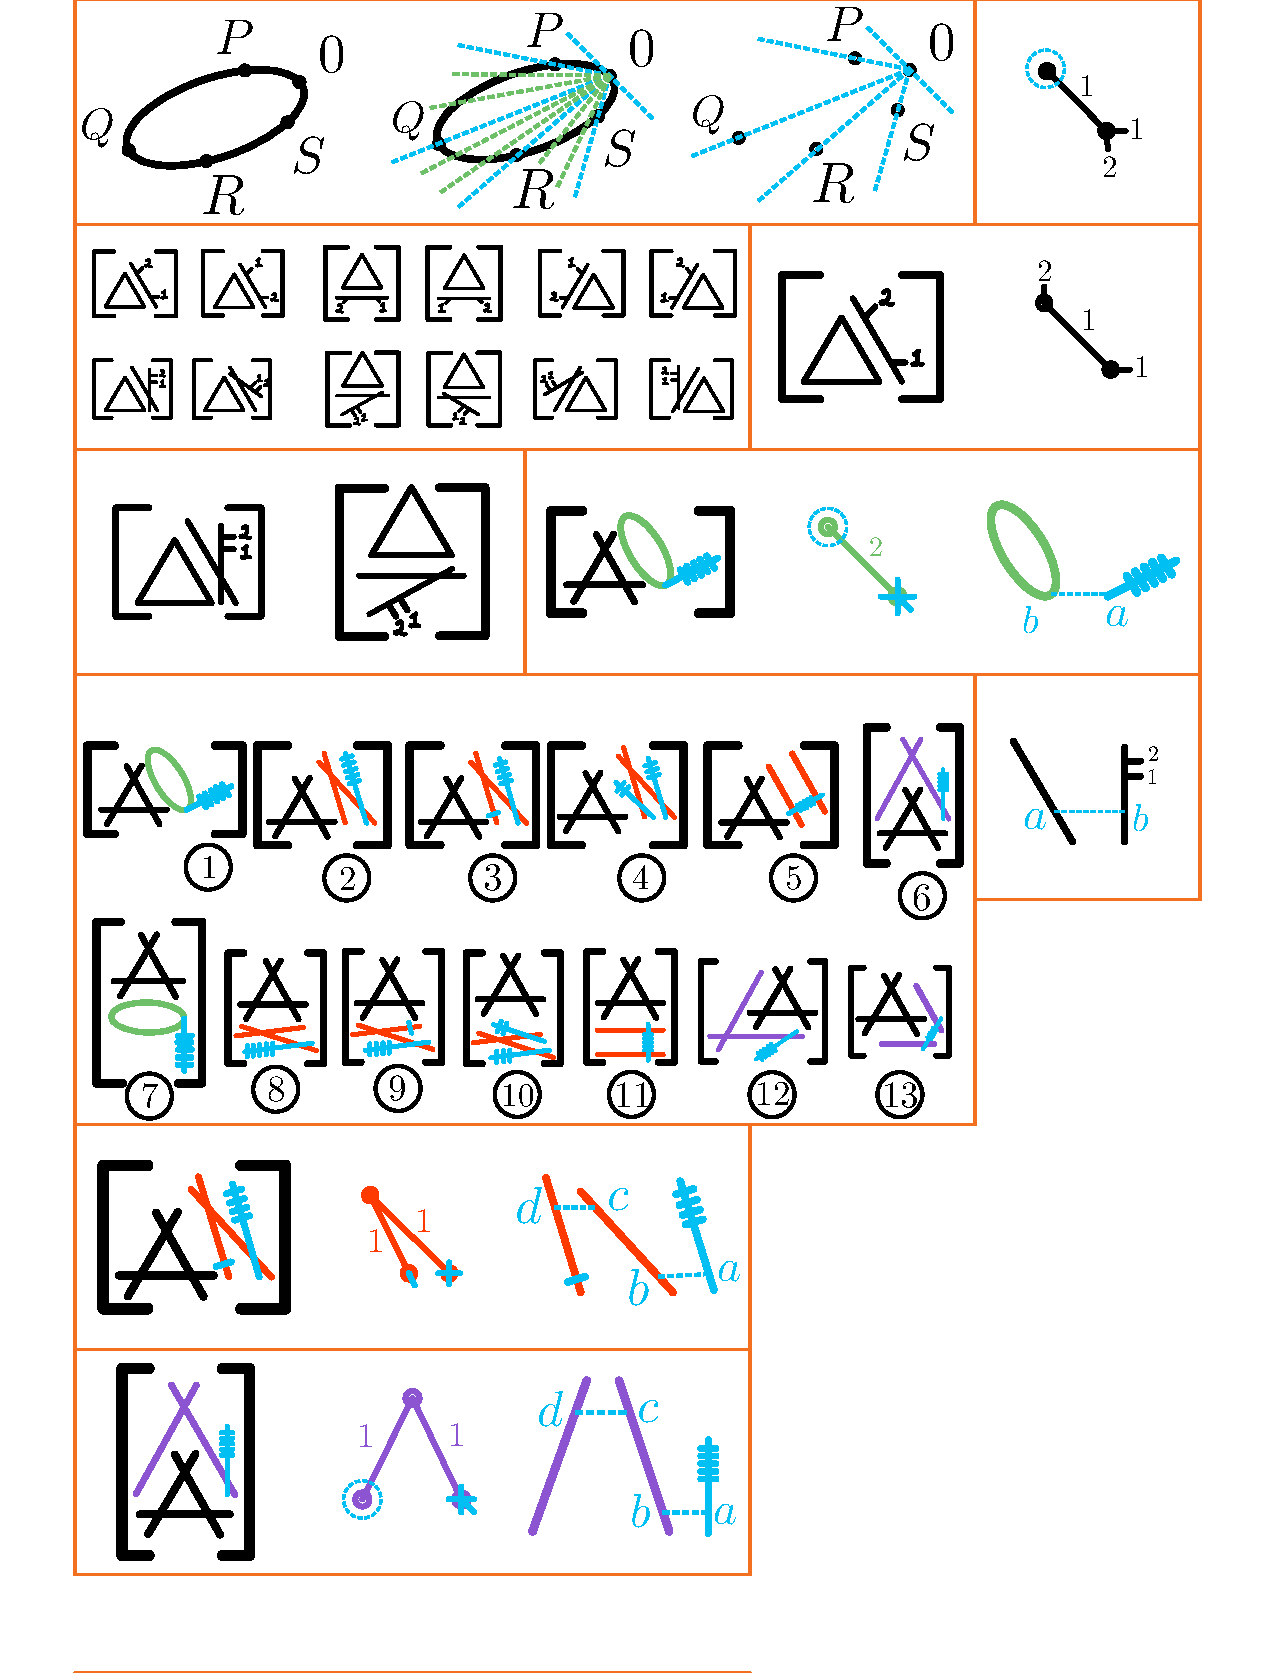
\includegraphics[width=0.7\textwidth, trim= 1.32cm 1.7cm 9cm 23cm,clip]{../figs/FigsDNnotability3.pdf}
        \caption{Loci $F_6$ along dual graph and normalization of source curve}
        \label{fig:quadratic-F6-5-marks}
    \end{figure}
    We proceed by analyzing the corresponding bundles.
    \begin{itemize}
        \item The dual graph contains only one vertex of valence one which maps to $[0:0:1]$. From this, we extract the Euler class of the automorphisms bundle to be 
        $$e(\Aut(C_6))=t_3-t_2.$$
        \item As in the last case, 4 points map to two nodes from which we obtain 
        \begin{align*}
            e(\DefB(C_6))&=(-\psi_a-\psi_b)(-\psi_c-\psi_d)\\
            &=(-\psi_a+(t_1-t_2))((t_2-t_1)+(t_2-t_3))\\
            &=(t_1-t_2)(2t_2-t_1-t_3)\left(1-\frac{\psi_a}{t_1-t_2}\right)
        \end{align*}
        Here $\psi_a$ is a psi-class on $\ov M_{0,6}$.
        \item For $F_6$, we run into the issue that node corresponding to $c$ and $d$ is being mapped onto \emph{both} lines $\set{X=0}$ and $\set{Z=0}$. This means that the process of decomposing the tangent bundle into two can no longer be done as we will arrive at an ambiguity. Still from the normalization sequence we obtain
        $$0\to\cO_{C_6}\to\cO_{C_{6,1}}\oplus\cO_{C_{6,2}}\oplus\cO_{C_{6,3}}\to\un\bC_{n_1}\oplus\un\bC_{n_2}\to 0$$
        but now we tensor by $-\ox\mu_6^\ast T\bP^2$ and take the long exact sequence in cohomology. This allows us to take weights in a similar fashion so that 
        \begin{align*}
             e(\DefB(\mu_6))&=\scriptstyle\frac{((t_3-t_1)(t_3-t_2))((t_2-t_1)(t_2-t_3))((t_2-t_3)(t_2-t_1))((t_1-t_3)(t_1-t_2))((t_1-t_3)(t_1-t_2))}{((t_2-t_1)(t_2-t_3))((t_1-t_3)(t_1-t_2))}\\
             &=((t_3-t_1)(t_3-t_2))((t_2-t_3)(t_2-t_1))((t_1-t_3)(t_1-t_2))\\
             &=-\bonj{(t_1-t_2)(t_1-t_3)(t_2-t_3)}^2
        \end{align*}
    \end{itemize}
    Joining everything into the Euler class, we expect it to have degree 7. Observe that 
    \begin{align*}
        e(N_{F_6\mid\ov M})&=\frac{-\bonj{(t_1-t_2)(t_1-t_3)(t_2-t_3)}^2\bonj{(t_1-t_2)(2t_2-t_1-t_3)\left(1-\frac{\psi_a}{t_1-t_2}\right)}}{t_3-t_2}\\
        &=(t_1-t_2)^3(t_1-t_3)^2(t_2-t_3)(2t_2-t_1-t_3)\left(1-\frac{\psi_a}{t_1-t_2}\right)
    \end{align*}
    does indeed have degree $7$ and so we now integrate to obtain
    \begin{align*}
        I_6&=\int_{F_6}\frac{p^5}{e(N_{F_6\mid\ov M})}\\
        &=\int_{\ov M_{0,6}}\frac{(t_1-t_3)^5(t_1-t_2)^5}{(t_1-t_2)^3(t_1-t_3)^2(t_2-t_3)(2t_2-t_1-t_3)\left(1-\frac{\psi_a}{t_1-t_2}\right)}\\
        &=\frac{(t_1-t_3)^3(t_1-t_2)^2}{(t_2-t_3)(2t_2-t_1-t_3)}\int_{\ov M_{0,6}}\frac{1}{1-\frac{\psi_a}{t_1-t_2}}\\
        &=\frac{(t_1-t_3)^3}{(t_1-t_2)(t_2-t_3)(2t_2-t_1-t_3)}\int_{\ov M_{0,6}}\psi_a^3\\
        &=\frac{(t_1-t_3)^3}{(t_1-t_2)(t_2-t_3)(2t_2-t_1-t_3)}.
    \end{align*}
    Finally $F_{13}$ has an entire component collapsing into a point. This will be treated similar as $F_6$'s node mapping to a point. We must construct the dual graph and normalization in order to proceed.\begin{figure}[h!]
        \centering
        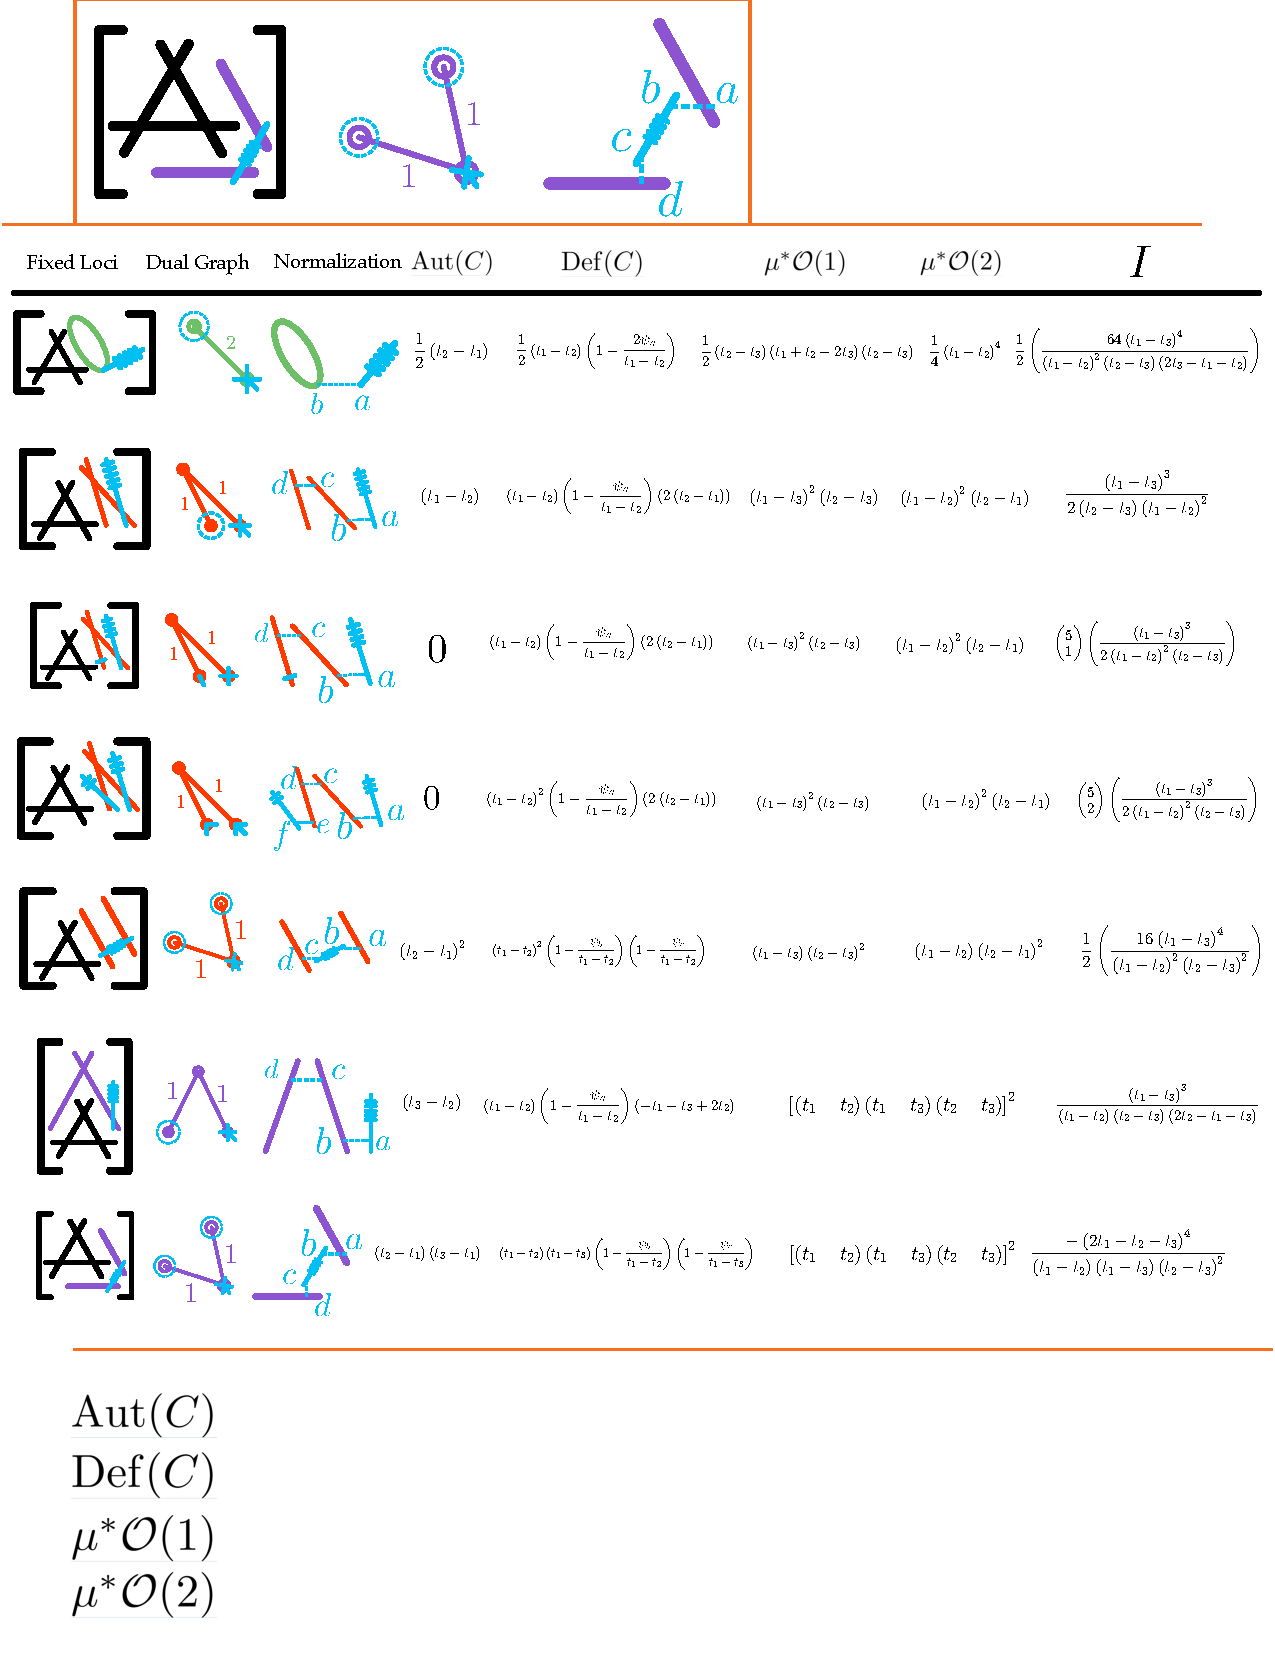
\includegraphics[width=0.7\textwidth, trim= 1.32cm 24.6cm 9cm 0.1cm,clip]{../figs/FigsDNnotability4.pdf}
        \caption{Loci $F_{13}$ along dual graph and normalization of source curve}
        \label{fig:quadratic-F13-5-marks}
    \end{figure}
    \begin{itemize}
        \item The dual graph has two valence one vertices from which we obtain two weights so that 
        $$e(\Aut(C_{13}))=(t_2-t_1)(t_3-t_1).$$
        \item As before, we have 4 points mapping to two nodes so that  \begin{align*}
            e(\DefB(C_{13}))&=(-\psi_a-\psi_b)(-\psi_c-\psi_d)\\
            &=((t_1-t_2)-\psi_b)(-\psi_c+(t_1-t_3))\\
            &=(t_1-t_2)(t_1-t_3)\left(1-\frac{\psi_b}{t_1-t_2}\right)\left(1-\frac{\psi_c}{t_1-t_3}\right)
        \end{align*}
        where $\psi_b$ and $\psi_c$ are psi-classes on the same $\ov M_{0,7}$. 
        \item Expanding out the normalization sequence  
        $$0\to\cO_{C_{13}}\to\cO_{C_{13,1}}\oplus\cO_{C_{13,2}}\oplus\cO_{C_{13,3}}\to\un\bC_{n_1}\oplus\un\bC_{n_2}\to 0,$$
        tensoring by $-\ox\mu_{13}^\ast T\bP^2$ and taking the long exact sequence in cohomology provides us with the Euler class. In a similar fashion as before, the part corresponding to $C_{13,2}$ will acquire the weights of $T\bP^2$ corresponding to $[1:0:0]$. From this
        \begin{align*}
             e(\DefB(\mu_{13}))&=\scriptstyle\frac{((t_3-t_2)(t_3-t_1))((t_1-t_2)(t_1-t_3))((t_1-t_3)(t_1-t_2))((t_1-t_3)(t_1-t_2))((t_2-t_3)(t_2-t_1))}{((t_1-t_3)(t_1-t_2))((t_1-t_3)(t_1-t_2))}\\
             &=((t_3-t_2)(t_3-t_1))((t_1-t_3)(t_1-t_2))((t_2-t_3)(t_2-t_1))\\
             &=-\bonj{(t_1-t_2)(t_1-t_3)(t_2-t_3)}^2.
        \end{align*}
    \end{itemize}
    The expected degree of the Euler class is the codimension of $\ov M_{0,7}$ which is $6$, observe that 
        \begin{align*}
        e(N_{F_{13}\mid\ov M})&=\frac{-\bonj{(t_1-t_2)(t_1-t_3)(t_2-t_3)}^2\bonj{(t_1-t_2)(t_1-t_3)\left(1-\frac{\psi_b}{t_1-t_2}\right)\left(1-\frac{\psi_c}{t_1-t_3}\right)}}{(t_2-t_1)(t_3-t_1)}\\
        &=-\bonj{(t_1-t_2)(t_1-t_3)(t_2-t_3)}^2\left(1-\frac{\psi_b}{t_1-t_2}\right)\left(1-\frac{\psi_c}{t_1-t_3}\right)
    \end{align*}
    The integral is 
    \begin{align*}
        I_{13}&=\int_{F_{13}}\frac{p^5}{e(N_{F_{13}\mid\ov M})}\\
        &=\int_{\ov M_{0,7}}\frac{(t_1-t_3)^5(t_1-t_2)^5}{-\bonj{(t_1-t_2)(t_1-t_3)(t_2-t_3)}^2\left(1-\frac{\psi_b}{t_1-t_2}\right)\left(1-\frac{\psi_c}{t_1-t_3}\right)}\\
        &=\frac{-(t_1-t_3)^3(t_1-t_2)^3}{(t_2-t_3)^2}\int_{\ov M_{0,7}}\frac{1}{\left(1-\frac{\psi_b}{t_1-t_2}\right)\left(1-\frac{\psi_c}{t_1-t_3}\right)}.
    \end{align*}
    Now, we must expand both terms as power series and analyze those terms which have degree 4. Observe that we have
    \begin{align*}
        \frac{1}{\left(1-\frac{\psi_b}{t_1-t_2}\right)\left(1-\frac{\psi_c}{t_1-t_3}\right)}&=\scriptstyle\left(1+\frac{\psi_b}{t_1-t_2}+\left(\frac{\psi_b}{t_1-t_2}\right)^2+\left(\frac{\psi_b}{t_1-t_2}\right)^3+\dots\right)\left(1+\frac{\psi_c}{t_1-t_3}+\left(\frac{\psi_c}{t_1-t_3}\right)^2+\left(\frac{\psi_c}{t_1-t_3}\right)^3+\dots\right)\\
        &=\dots+\sum_{k=0}^{4}\left(\frac{\psi_b}{t_1-t_2}\right)^k\left(\frac{\psi_c}{t_1-t_3}\right)^{4-k}+\dots\\
        &=\dots+\sum_{k=0}^{4}\left(\frac{1}{t_1-t_2}\right)^k\left(\frac{1}{t_1-t_3}\right)^{4-k}\psi_b^k\psi_c^{4-k}+\dots\\
        \To\int_{\ov M_{0,7}}\frac{1}{\left(1-\frac{\psi_b}{t_1-t_2}\right)\left(1-\frac{\psi_c}{t_1-t_3}\right)}&=\dots+\sum_{k=0}^{4}\left(\frac{1}{t_1-t_2}\right)^k\left(\frac{1}{t_1-t_3}\right)^{4-k}\int_{\ov M_{0,7}}\psi_b^k\psi_c^{4-k}+\dots\\
        &=\sum_{k=0}^{4}\left(\frac{1}{t_1-t_2}\right)^k\left(\frac{1}{t_1-t_3}\right)^{4-k}\binom{4}{k}\\
        &=\left(\frac{1}{t_1-t_2}+\frac{1}{t_1-t_3}\right)^4=\left(\frac{2t_1-t_2-t_3}{(t_1-t_2)(t_1-t_3)}\right)^4.
    \end{align*}
    Replacing this term into our last expression leaves us with the final result for $I_{13}$
    $$I_{13}=\frac{-(t_1-t_3)^3(t_1-t_2)^3}{(t_2-t_3)^2}\left(\frac{2t_1-t_2-t_3}{(t_1-t_2)(t_1-t_3)}\right)^4=\frac{-(2t_1-t_2-t_3)^4}{(t_1-t_2)(t_1-t_3)(t_2-t_3)^2}.$$
    Following this process we may summarize the calculations with the following table.
    \begin{figure}[h!]
        \centering
        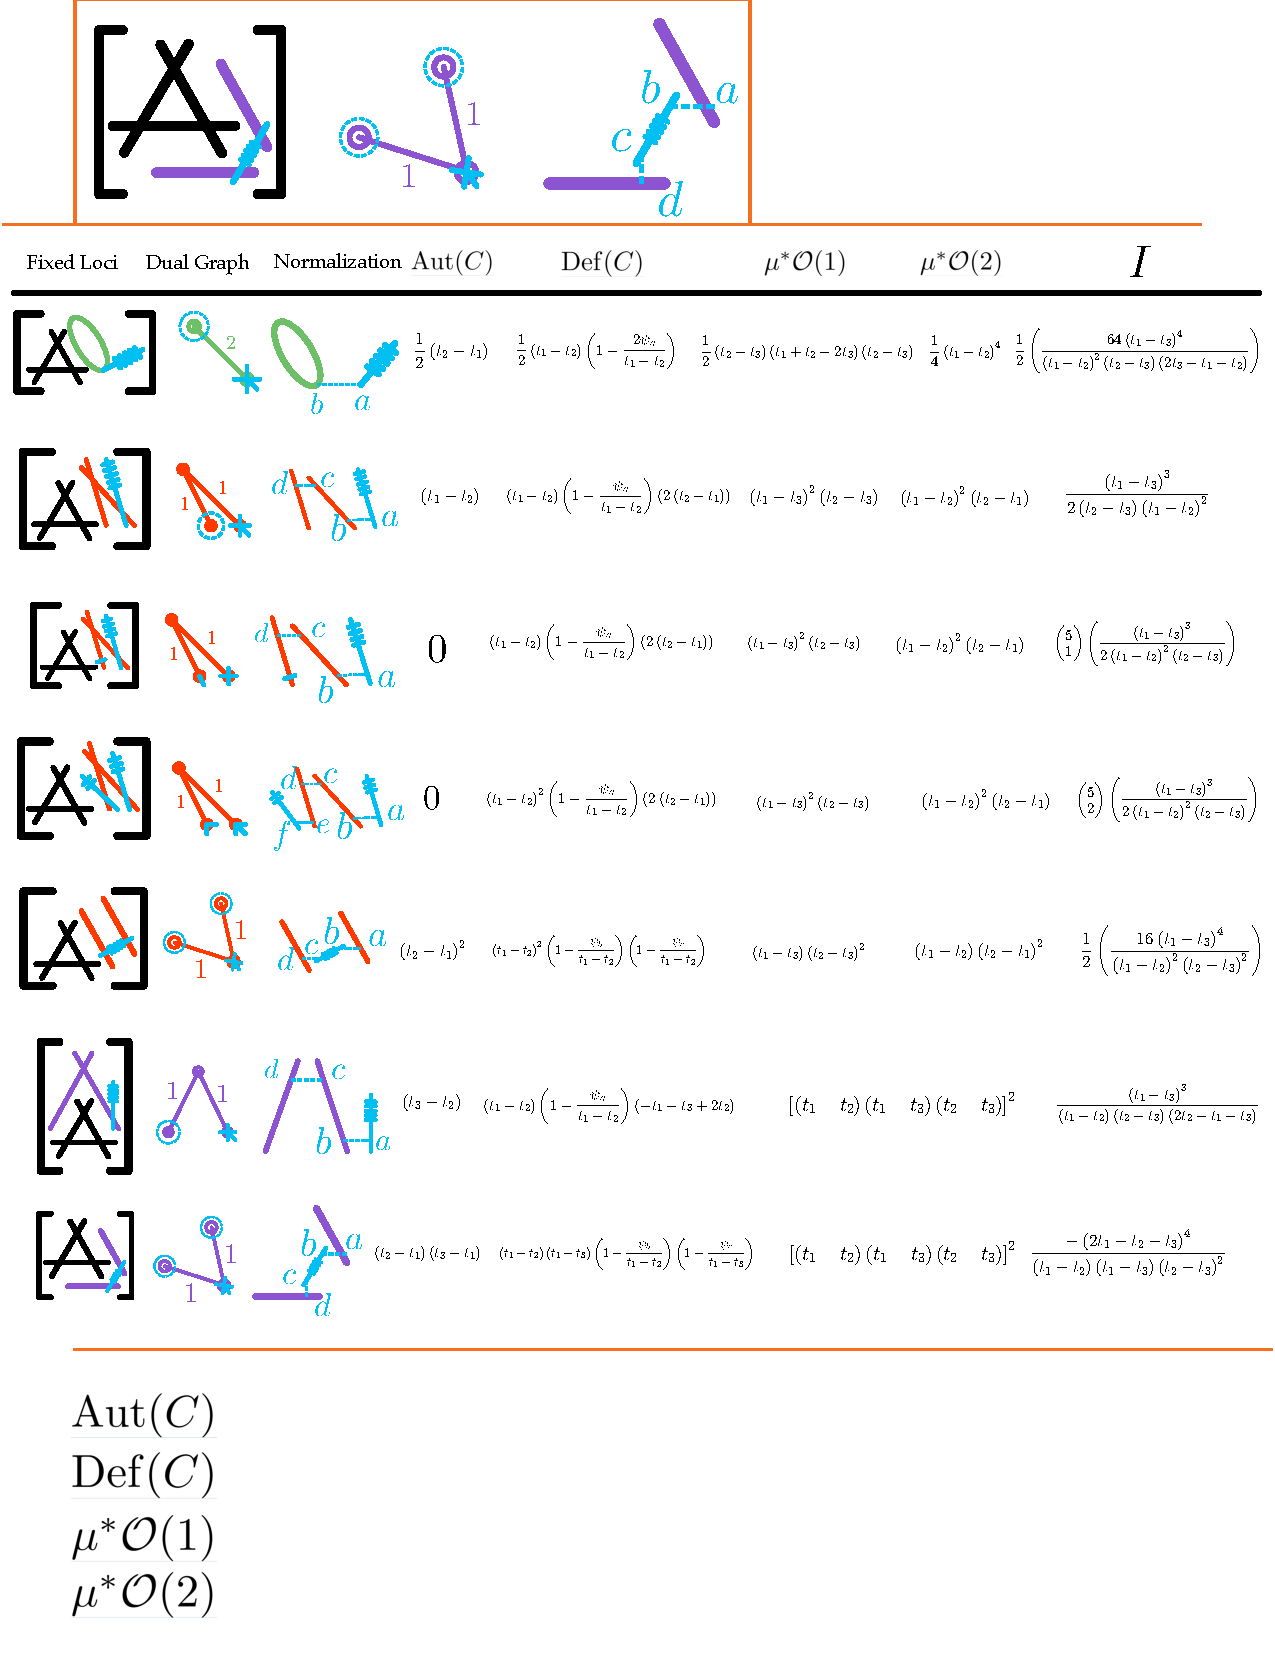
\includegraphics[width=1\textwidth, trim= 0.1cm 6cm 0.1cm 4.1cm,clip]{../figs/FigsDNnotability4.pdf}
        \caption{Summary of integrals for $\ov{M}_{0,5}(\bP^2,2)$}
        \label{fig:summary-table-M05P22}
    \end{figure}
    Summing up all terms along with mirror images via the action $(23)\.$ we do get one which is the number of conics passing through 5 points.
\end{Ex}
Observe that in the same fashion as in example \ref{ex:N1-different-points}, distributing the marks throughout the fixed points in $\bP^2$, reduces the number of fixed loci to work with. Taking the integral 
$$\int_{\ov{M}_{0,5}(\bP^2,2)}\ev_1^\ast([1:0:0])\ev_2^\ast([1:0:0])\ev_3^\ast([0:1:0])\ev_4^\ast([0:1:0])\ev_5^\ast([0:0:1])$$
produces the same result with only a count of 3 fixed loci. The reader may be interested in pursuing this exercise on their own account.\par
We have also applied the following lemma several times, it simplifies the contribution of psi-classes to the curve deformations bundle.

\begin{Lem}
    For $\psi,\widetilde\psi$ psi-classes in $\ov M_{0,n}$, it holds that
    $$\int_{\ov M_{0,n}}\frac{1}{(1-\frac{\psi}{x-y})(1-\frac{\widetilde\psi}{x-z})}=\left(\frac{1}{x-y}+\frac{1}{x-z}\right)^{n-3}.$$
\end{Lem}
\section{Future directions}

In this work we have developed the ideas of equivariant cohomology and localization, focusing on applying them to the moduli space of stable maps. Along the theory of moduli space of curves, we have the necessary tools to approach other moduli spaces to which we may apply these techniques.\par
Looking ahead, the direction is to extend these methods to alternate moduli spaces. In particular, we aim to study \emph{pseudo}-stable curves and the analogous space of maps. 
%%%%%%%%%%%% Contents end %%%%%%%%%%%%%%%%
\ifx\nextra\undefined
\printindex
\else\fi
\nocite{*}
\bibliographystyle{plain}
\bibliography{bibiTM.bib}
\end{document}